%!TEX TS-program = xelatex 
%!TEX encoding = UTF-8 Unicode

% Modify the following line to match your school
% Available options include `Harvard`, `Princeton`, and `NYU`.
\documentclass[School=Harvard]{Dissertate}
\usepackage[round,authoryear]{natbib}
%\usepackage[backend=biber,style=authoryear,sorting=nyt,sortcites=true]{biblatex}
%\addbibresource{references.bib}

\setcounter{secnumdepth}{3}
\usepackage{enumitem}
\usepackage{imakeidx}
\makeindex
%\usepackage[tagged, highstructure]{accessibility}

%======for 3D Torus=====%
\usepackage{tikz} % For creating graphics
\usepackage{pgfplots} % For plotting 3D points
\pgfplotsset{compat=1.17} % Ensures compatibility with pgfplots version 1.17
\usetikzlibrary{3d, calc} % For 3D graphics and coordinate calculations
\interfootnotelinepenalty=10000 %Added 2025 Jan 11
\raggedbottom %Added 2025 Jan 11


%======for Âhasiw Maskêgon-Iskwêw =====%


\begin{document}
% the front matter
% Some details about the dissertation.
\title{What may be known: methods for activating large texts and graphs in the climate crisis}
\author{Orus Mateo Castaño-Suárez}
\advisor{Dr. A. Tindale and G. Van Alstyne}

% ... about the degree.
\degree{Master of Arts}
\field{Digital Futures}
\degreeyear{2025}
\degreemonth{December}
\department{Digital Futures}

% ... about the candidate's previous degrees.
% \pdOneName{B.S.}
% \pdOneSchool{Example University}
% \pdOneYear{2018}

% \pdTwoName{M.A.}
% \pdTwoSchool{Example Univeristy}
% \pdTwoYear{2021}

\maketitle

\OpenResearchPage
\copyrightpage
\doublespacing
\dedicationpage
\abstractpage
\tableofcontents
\addcontentsline{toc}{chapter}{Table of Contents}

\listoffigures
\addcontentsline{toc}{chapter}{List of figures}
\clearpage




\listoftables
\addcontentsline{toc}{chapter}{List of tables}
\clearpage %added 2025 Jan 15
\FloatBarrier

\abbreviations
\clearpage

\antistatement
\clearpage

\AI
\clearpage

\landack
\clearpage

\professionalack
\clearpage

\personalack
\clearpage

\acknowledgments
\clearpage
%
\noindent This thesis was supported by Canada's Ontario Graduate Scholarship, the St. George’s Society of Toronto, OCAD University, the William and Phyllis Waters Bursary, Nodus Labs, the Institute for Equitable Design and Justice, the Open Education Conference, and SimFoto.
%\ENDOR
\affiliation
\clearpage

%\acknowledgments
\doublespacing
% include each chapter...
%\setcounter{chapter}{-1}  % start chapter numbering at 0
%\include{chapters/introduction}
	\setcounter{page}{1}
	\pagenumbering{arabic}
%\begin{savequote}[75mm]
%Nulla facilisi. In vel sem. Morbi id urna in diam dignissim feugiat. %Proin molestie tortor eu velit. Aliquam erat volutpat. Nullam ultrices, diam tempus vulputate egestas, eros pede varius leo.
%\qauthor{Quoteauthor Lastname}
%\end{savequote}
%methodological prototype
%Experiments in Information visualization as anticipatory designs of visuospatial topic modelling, made as a means of climate crisis mitigation and accelerating interdiscipilinary research as a whole.
%I demonstrate my methodological prototype's function through interface mockups, i.e. Ch 5
\chapter{Introduction}

We are in a crisis of understanding. The magnitude and complexity of the climate crisis and its many related crises demand that we change the tools and methods we use to think. This thesis proposes a novel framework for activating large texts, particularly in the critical domain of climate resilience. In this thesis, I propose a response to the climate crisis that builds on the ways we reason with symbols and graphs as a means to accelerate interdisciplinary knowledge work. 
\index[terms]{climate resilience}

The climate crisis is accelerating, which imposes a shrinking timeline for innovating ways to face it. Furthermore, while we may need to create new tools and methods, we may already have solutions for climate crisis mitigation that lie inactive in the silos of research repositories and their marginalia.

My thesis positions itself at the intersection of urgent global need and emerging technological possibility. At a moment in history when time saved in research could mean the survival of innumerable humans and other forms of life, the development of better ways to work with knowledge could hardly be more urgent. 

\section{Background and context}

\subsection{Research Problems and Significance}

Our crisis of understanding demands new solutions, and fast. However, the growing amount of information makes it impossible to consider all data. As Drucker notes, ``The expansion of access to any and all stored data that can be repurposed and remediated nearly boggles the mind” \citep[p. 194]{drucker_graphesis_2014}.
\index[people]{Drucker, Johanna}

Working through all available information in every discipline to find climate resilience solutions is likely impossible or would require an unsustainable amount of time and resources. The endeavour of ``developing the ability to cope with much larger amounts of information" \citep[p. 34]{sevaldson_designing_2022} can and should include developing tools that increase the efficiency of managing information complexity and facilitate conceptual translation between disciplines. Knowledge Activation, or activating connections between disciplines using computationally assisted methods of analyzing text and graphs, has the earth-changing potential to reveal solutions to global issues like the climate crisis. Paradigm-shifting solutions for climate resilience almost certainly exist already, and it is critical that we endeavour to find and apply them. Some new knowledge production will inevitably be necessary to minimize harm during Sustainability Transitions, but we may only need to activate the knowledge we already have.
\index[people]{Sevaldson, Birger}
\index[terms]{climate resilience}

\subsection{Foundations of key ideas}

\subsubsection{Isomorphism}
%Alternative thesis title: Data isomorphism and the climate crisis
Computational tools can accelerate climate resilience knowledge work in many disciplines. However, the magnitude of addressing global climate requires integrating disciplinary approaches for solutions that have yet to be imagined. In addition to being curious researchers, we must proactively interpret the shape of knowledge and identify latent solutions that fit key-in-lock into challenges of our primary disciplines, from within and outside our areas of expertise. By developing systems that help interpret the shape of information, we can more quickly find `keys' with the form we need for a given `lock'.

In my analogy of keys, this sameness of form is also called isomorphism as coined by chemist Eilhard Mitscherlich in the early 19th century
\citetext{\citealp[p. 239]{Berzelius1821Loethrohr}; \citealp{the_editors_of_encyclopaedia_britannica_eilhardt_2024}; \citealp [p. 427-437]{Mitscherlich1820Abhandlungen}; \citealp[p. 239]{Mitscherlich1837Lehrbuch1}}. The word isomorph is composed of the Greek words \textit{ἴσος} (\textit{ísos}, ‘equal’) and \textit{μορφή} (\textit{morphḗ}, ‘form’) \citetext{%
  \citealp[s.v.~\textit{ἴσος}]{liddell__1996-5}; %
  \citealp[s.v.~\textit{μορφή}]{liddell__1996-6}%
}.
\index[people]{Mitscherlich, Eilhard}
\index[terms]{isomorph}
\index[terms]{isomorphism}



\subsubsection{Data}
 To continue development of tools for data isomorphism, and further co-inform ``engineering capability with an imaginative sensibility" \cite[p. 195]{drucker_graphesis_2014} in `\textit{humanistic} forms of knowledge production" \citep[p. 10]{drucker_graphesis_2014}, we must contend with the ontological and epistemological implications of approaching knowledge with word \textit{data,} informed by its etymology.

The conventional use of the English word data traces to Latin \textit{datum} (‘something given, granted’) \citep{oxford_english_dictionary_datum_2024}, which de-emphasizes the interpretive agency of the receiver. By contrast, \textit{capta} (‘things taken’) derives from Latin \textit{capere} (‘to take, receive, acquire’) \citep{ashdowne_capere_2013}, shifting agency toward the receiver’s choice in working with knowledge.
\index[terms]{capta}
\index[terms]{data}

Drucker defines capta as ``a systematic expression of information understood as constructed, as phenomena perceived according to principles of observer-dependent interpretation" \citep[p. 131]{drucker_graphesis_2014}. Drucker adds that by ``qualifying any metric as a factor of some condition, the character of the ``information” shifts from self-evident ``fact” to constructed interpretation motivated by a human agenda" \citep[p. 131]{drucker_graphesis_2014}.

In my thesis, I apply the term \textit{capta} in key anchor terms. For example, to refer to Topological \textit{Data} Analysis (TDA), I propose the term Topological \textit{Capta} Analysis (TCA) instead. Although I generally agree with using the term \textit{capta} and its emphasis on interpretative knowledge construction, I deemed it impractical in writing this thesis to adapt each quotation that uses the term data, due to the broad range of discussions and sources I chose. For this reason, most quotations which use the word data are included without renaming or additional comment. Nevertheless, while I value the disambiguation of data and capta, my experience of knowledge involves a combination of both how I am changed by the `given-ness' events (data) \textit{and} my active interpretation of those events (capta).


\index[terms]{Topological Data Analysis (TDA)}
\index[terms]{Topological Capta Analysis (TCA)}
\index[terms]{capta}
\index[terms]{data}
%\index[terms]{humanistic forms of knowledge production}

\subsection{Research Questions}

Working within this background and context, I ask the following primary research question and seven secondary research questions:

\begin{enumerate}
    \item[\textbf{RQ1}] \textit{What philosophical, mathematical, and computational approaches to textual/graphical analysis can accelerate knowledge work?}
    \item[\textbf{RQ1.1}] \textit{What forms of spatial information visualization are there, and how can they inform the composition of network graphs?}
    \item[\textbf{RQ1.2}] \textit{How can Computational Analysis of Texts and Graphs (CATG) identify isomorphic semantic structures within large network graphs?}
    \item[\textbf{RQ1.3}] \textit{What methods can reveal the relationships between fundamental ideas in texts, graphs, or Large Language Models (LLMs)?}
    \item[\textbf{RQ1.4}] \textit{Given the semantic versatility of symbols, how can a practice of collaborative symbol-making support knowledge production?}
    \item[\textbf{RQ1.5}] \textit{How can CATG reveal relationships between place and text?}
    \item[\textbf{RQ1.6}] \textit{What strategies can improve university knowledge management to accelerate research?}
    \item[\textbf{RQ1.7}] \textit{What sort of knowledge work software would I want to build to incorporate my various findings and use spatial information visualization to identify isomorphic semantic structures, reveal the relationships between fundamental ideas, build on collaborative symbol-making, reveal relationships between place and text, and improve university knowledge management?}
\end{enumerate}


\subsection{Thesis Statement and Contributions}

The climate crisis continues to accelerate faster than climate resilience research and operationalization can keep up. Novel approaches for Knowledge Activation can catalyze paradigmatic shifts in Sustainability Transitions (ST). The seven contributions of this thesis are a set of such novel approaches proposed for visuospatial Knowledge Activation (KA) using human-in-the-loop (HITL) Computational Analysis of Texts and Graphs (CATG), Human Analysis of Texts and Graphs (HATG), or both. These seven contributions would be used for the surfacing, synthesis, translation, and production of knowledge:
\index[terms]{climate resilience}

\begin{enumerate}
    \item[\textbf{C1}] \textit{Semantic Forms}, a taxonomy of three-dimensional topic model compositions for HITL CATG, HATG, or both.
    \item[\textbf{C2}] \textit{Query Isomorphs} as a means of Topological Capta Analysis (TCA) in HITL CATG using small graph chunks.
    \item[\textbf{C3}] \textit{Ontological Semantic Network Summaries (OSNS)} as a means of revealing ontological relationships between ideas in a given body of research using HITL CATG, HATG, or both.
    \item[\textbf{C4}] \textit{Symbol-setting}, a method for expanding the semiotic range of knowledge production using symbol co-creation in HITL CATG, HATG, or both.
    \item[\textbf{C5}] \textit{Terroir of Text and Graphs (TTG)}, a method of HITL CATG that uses TCA to interpret and reveal semantic relationships between (a) texts and graphs, and (b) the features and systems of ecological place.
    \item[\textbf{C6}] \textit{TCA Researcher Grouping}, a proposal to use TCA for grouping research collaborators more effectively using HITL CATG, HATG, or both; finally,
    \item[\textbf{C7}] \textit{TCA Workspace}, a methodological prototype of a collaborative platform for HITL CATG and HATG to:
    \begin{enumerate}
        \item[(a)] integrate all my thesis contributions (\textit{Semantic Forms}, \textit{Query Isomorphs}, \textit{OSNS}, \textit{Symbol-setting}, \textit{TTG}, and \textit{TCA Researcher Grouping}).
        \item[(b)] facilitate computational interface with Systemic Design methods for visuospatial reasoning encountered through my literature review, such as gigamapping 
        \citetext{\citealp{sevaldson_giga-mapping_2011}; \citealp[p. 26]{sevaldson_designing_2022}} and Systematic Combining \citetext{\citealp[p.554]{dubois_systematic_2002}, \citealp{kjode_entanglement_2024}}.
    \end{enumerate}
\end{enumerate}
\index[people]{Gadde, Lars-Erik}
\index[people]{Dubois, Anna}
\index[terms]{gigamapping}
\index[terms]{Systematic Combining (SC)}
        

The core of this thesis is a set of two method proposals for working with graphs of text, Semantic Forms and Query Isomorphs, integrated into one methodological prototype: TCA Workspace. Developing the TCA Workspace software platform has the potential to accelerate the surfacing and interpretation of interdisciplinary climate resilience knowledge using the computational analysis of texts and graphs. TCA Workspace would integrate Semantic Forms for the three-dimensional modelling of text graphs, Query Isomorphs for Topological Capta Analysis, and interdisciplinary symbolic co-creation as Symbol-setting. Furthermore, TCA Workspace would work co-benefit existing Systemic Design methods for managing complexity including gigamapping \citetext{\citealp{sevaldson_giga-mapping_2011}; \citealp[p. 26]{sevaldson_designing_2022}}, and Systematic Combining \citetext{\citealp{dubois_systematic_2002}; \citealp{kjode_entanglement_2024}}. Epistemologically, TCA Workspace would function as a particle accelerator of ideas, where researchers would work with texts and graphs as activated webs of thought.
\index[terms]{gigamapping}
\index[terms]{Systematic Combining (SC)}
\index[people]{Gadde, Lars-Erik}
\index[people]{Dubois, Anna}
\index[terms]{climate resilience}

\FloatBarrier
\begin{figure}[ht]
    \centering
    \includegraphics[width=\textwidth]{figures/5.16.HT1.png}
    \caption[Preview of TCA Workspace illustrations]{\textbf {Preview of TCA Workspace illustrations.} Horn Torus Semantic Form about Query Isomorph \textit{i}. Render of how TCA Workspace would render a Query Isomorph about this thesis located in a Horn Torus Semantic Form network graph.}
    \label{f5.16.HT1}
\end{figure}



\FloatBarrier
\clearpage



\subsection{My prior work}

My prior work in education technology and theological academia frames the epistemological diversity that motivates and informs this thesis.

Building on my research in EdTech UX design, branding, and creative direction, my approach expanded to include the use of design tools for managing operations. For example, I developed and implemented organizational resource maps to minimize lag in sharing multimedia assets within and between departments. I then expanded these resource management systems so they could also maps of organizations' written resources, like official company copy and positioning research. By visualizing the relationships of information within organizations I activated the knowledge that already existed in company assets, empowering all departments independently, while working better as a whole. 

In parallel, my engagement with theological research and art-making, particularly within the Harvard Divinity School Program for the Evolution of Spirituality art and spirituality working group, centred the themes of power and climate grief. In my exhibition \textit{Song Within a Sacrifice Zone}, and the artist talk and interview that followed, I grappled with the grief and disorienting overwhelm of the global warming crisis \citep{1496711,castano-suarez_biopower_2023,castano-suarez_song_2023-1}. Furthermore, in my presentation on biopower and the pastorate, and the subsequent panel discussion, I addressed abuses of power and the anti-oppressive potential of emerging information management techniques \citep{1496651,castano-suarez_biopower_2023,castano-suarez_biopower_2024}.

Ultimately, my prior work in design leadership pointed me to the need for more robust methods to organize information across groups of people who think and work differently from each other. This thesis addresses the innovation of methods more directly, representing an expansion of both the scale and semantic scope of my earlier work in organizational information mapping practice, all oriented in service of anti-oppressive climate resilience.
\index[terms]{climate resilience}
\index[terms]{climate justice}



\section{How this thesis is organized}

The overall structure of my thesis is as follows: In the following chapters, this thesis will move from a literature review to secondary methodologies and methods, preliminary work, visuospatial models derived from theory, methodological and theoretical proposals derived from visuospatial models, a reflection on the literature review, a discussion of my contributions, and a conclusive call to action. 

In Chapter 1, I introduced my thesis's background and context, research problems and significance, foundations of key ideas, research questions, thesis statement, contributions, and prior work.

In Chapter 2, Literature review, I present my mixed-methods scoping review. I frame the review with information about the climate crisis and various cognitive and social challenges it represents. I then present ways that approaches from design and computer science can help manage complexity. I then critique the terms ``blind-spots," ``black box AI," and ``stakeholders." I end my identifying the gaps I observed in my literature review.

In Chapter 3, Secondary methodologies and methods, I present how I worked within the Research-Creation and Critical Systems Methodologies. Here, I present my methods, sampling strategy, and analytical approaches, including Systematic Combining and Meta-Systematic Combining. 

In Chapter 4, Preliminary making, I present the art and design thought experiments that catalyzed this thesis: the composition of horn torus spatial information visualization. Next, I present my code and information analysis experiments in Personal Knowledge Management, topic models, and Small Language Models. 

In Chapter 5, From theory and method to visuospatial models and back, I present the ways Semantic Forms, Query Isomorphs, and how they work together. Next, I present TCA Workspace. Last I present the theoretical and methodological contributions I arrived at through making visuospatial models: Ontological Semantic Network Summaries (OSNS), Symbol-setting, Terroir of Text and Graphs, and TCA Researcher Grouping. 

In Chapter 6, Discussion of contributions, I retrace my research questions and present how my contributions respond to each.In this section, I also present the humanist post-structuralist design and multi-mathematical qualities of Semantic Forms, Query Isomorphs, OSNS, Symbol-setting, TTG, TCA Researcher, and the TCA Workspace platform overall.

In Chapter 7, Conclusion, I retrace the core problems I faced with research questions, present concluding syntheses, and offer a call to action.
%\begin{savequote}[75mm]
%This is some random quote to start off the chapter.
%\qauthor{Firstname lastname}
%\end{savequote}

\chapter{Literature review}
To address the compound crises of climate and information, we must produce new knowledge and activate existing knowledge from various disciplines. Solutions to the climate crisis may already exist but remain hidden in the overwhelming amount of information available. To rethink how we integrate knowledge, we must take an interdisciplinary approach.

\section{Type of literature review}
Following Grant and Booth’s typology of reviews \citep[p. 91-108]{grant_typology_2009}, my thesis research uses mixed methods and a scoping review.

\subsection{Mixed methods review}
%\noindent \textbf{Mixed methods review} \\
As a mixed methods review, I combine quantitative and qualitative research from different fields. My research project is an example of how mixed methods reviews should be, by their nature, interdisciplinary, which means they analyze various disciplines. Drawing from philosophy, computer science, and mathematics, I examine a ``correlation between characteristics” to identify gaps in areas of literature \citep[p. 94]{grant_typology_2009}. In my research, I was unable to find studies, methods or platforms that propose or accomplish the following tasks simultaneously:
\begin{enumerate}
    \item[-] Distinguishing the various modalities of knowledge and ranks them by their expense, including distinct definitions between modes of Knowledge Activation, including Surfacing, Synthesis, Translation, and Production. The limited subtlety in this subject makes climate resilience research more costly than it needs to be. It is imperative to distinguish and quantify the expense of various modalities of Knowledge Activation by their expense to reduce unnecessary costs in climate resilience research.
\item[-] Distinguishing three-dimensional forms by the various ways they capture and reveal reasoning and other semantic relationships as layouts for text graphs and graph chunks. The limited research in this area restrains exploration of Visuospatial Knowledge Activation in various fields, including neuroscience, learning psychology, and design. Visuospatial models facilitate understanding because they capture and reveal reasoning and semantic relationships in text graph composition and graph chunks.
\item[-] Distinguishing how capturing and revealing semantic relationships in text graphs can be distinctly non-computational with the \textit{option} of being computational. In other words, I am pursuing solutions that do not impose but rather offer the option for computational analysis of texts and graphs (CATG), which keep humans in the loop (HITL). The limited distinction and combination of computational machine-driven and human-driven ‘manual’ methods in the visuospatial modes of Knowledge Production (a) hinders the use of valuable training data for LLMs that can support climate resilience research, (b) demonstrates that the practical applications of existing visuospatial modes of Knowledge Production lack a strong connection to research findings that indicate its value, and (c) limits the ways valuable technology can be used by climate resilience researchers. We must distinguish human-driven and machine-driven modes of VKA to take better advantage of each mode and the effectiveness of their combined use.  
\item[-] Deployment of contemporary tools for the non-computational Human Analysis of Texts and Graphs (HATG) that relies on manual placement of words and visual elements in three-dimensional space (e.g. Systemic Design, Systems Oriented Design, Systematic Combining, Boundary Critique). The limited options in this area prevent us from using the full range of our human ability to reason in visuospatial modes of Knowledge Activation and the optical opportunities beyond the restrictions of two-dimensional information representation. We must build better tools for non-computational HATG using manual placement in three-dimensional space to more fully apply the creative potential of human VKA beyond two-dimensional limits.
\item[-] Methods that use HATG to train algorithms or LLMs. We must drive research in this area to increase the impact of LLMs in climate resilience research and overall research. 
\end{enumerate}
\index[terms]{Visuospatial Knowledge Activation (VKA)} \index[terms]{Systemic Design} \index[terms]{Large Language Model (LLM)}
\index[terms]{Systematic Combining (SC)}
\index[terms]{Knowledge Production (KP)}
\index[terms]{composition}
\index[terms]{Systems Oriented Design (SOD)}
\index[terms]{Boundary Critique}
\index[terms]{climate resilience}

\subsection{Scoping review}
%\noindent \textbf{Scoping review} \\
For my scoping review, I used a keyword search across various databases, including the terms information visualization, visuospatial, personal knowledge management, digital scholarship, and others. 

To select the papers I read, I optimized for the depth of the coverage of each subject, opting for longer papers and publications whenever possible. I favoured primary research, which included more reflective pieces and experimental, qualitative, quantitative, and mixed-methods studies in various fields of mathematics and science, including systematic reviews. 

I aimed to assess the ``potential size and scope of available research” projects \citep[p. 95]{grant_typology_2009}. In doing so, I investigated whether any existing projects modelled the categorization of large groups of highly influential ideas in three-dimensional forms. Notably, I found only one example: Brian Sunter’s Wikipedia graphs \citep{sunter_organizing_2022, sunter_3d_2023}. 

I extended the scoping review method with a step recommended in systematic reviews, which often include a quality assessment step that inspired me to include recommendations for future research based on what remains unknown \citep[p. 95]{grant_typology_2009}. However, I cannot claim to propose what is \textit{not} known; only what I suggest \textit{may} be known. 

\section{Climate crisis: what is at stake}
Despite the misinformation about climate change, there is a nearly complete consensus that human causes are to blame \citep{Cook_2016,lynas_greater_2021}. According to Pörtner et al., none of the twenty ``2011–2020 Aichi biodiversity targets and none of the mileposts on climate trajectories intended to limit warming to 1.5°C have been met” \citep[p. 1]{portner_overcoming_2023}. The World Meteorological Organization (WMO) reports that the “past nine years, 2015–2023, were the nine warmest years on record” \citep[p. 3]{world_meteorological_organization_state_2024}. Despite this, greenhouse gas emissions continue to increase and “now exceed 55 billion tonnes of carbon dioxide equivalents” per year \citep[p. 1]{portner_overcoming_2023}. Critical life-saving targets have not been met, and yet humanity continues to increase its greenhouse gas emissions.

Our outlook is bleak if we do not work together. If the root causes of climate change and biodiversity loss are not met with a plan of action, global sustainability targets will continue to fail. We need radical collective action that addresses ``climate, biodiversity, and society” together, which ``can help to avoid dangerous trade-offs and maximize cobenefits for humankind” \citep[p. 1]{portner_overcoming_2023}. To ensure a livable future, we urgently need bold policies that better steward ``interlinked human, ecosystem, and planetary health” through coordinated social systems, institutions, and governance at local and global levels \citep[p. 1]{portner_overcoming_2023}. If we want a chance of avoiding much larger consequences to global warming, many more of us need to think more critically about our relationship to the larger web of life and its ecosystems. 

New large-scale solutions are required, and fast. The changes required to achieve the aims of the United Nations Framework Convention on Climate Change (UNCCC), the Convention on Biological Diversity (CBD), and the United Nations (UN) 2030 Agenda for Sustainable Development and its Sustainable Development Goals ``will rely on far-reaching mobilization and transformation actions of a type never before attempted” \citep[p. 8]{portner_overcoming_2023}. We need new solutions for global warming because we need to ``keep global warming below 1.5°C [...] to secure a livable future” \citep[p. 8]{portner_overcoming_2023}. 

To develop solutions that address the many aspects involved in global warming by working together across differences of disciplinary expertise is inevitable. In this way, this thesis is an investigation of how the development of technological research accelerators could allow us to find and implement more and better ways of stewarding our web of life. 



\section{Sociopolitics}
Clinging to the hope that we are yet discussing humanities and not posthumanities, I posit that the climate crisis is a crisis of understanding, institutionally and socially. 

%\noindent \textbf{Climate-related social change} \\
Applied climate-related understandings inevitably need to escalate the rate of collective social transformation if we want to minimize loss of life. 

Pörtner et al.'s review summary on societal impacts of sustainability polycrisis uses the term “social tipping” to refer to targeted interventions that cause self-reinforcing momentum ``with positive impacts on climate, biodiversity and human well-being" \citep[p. 7]{portner_overcoming_2023}. Building tools for managing complexity and inter/multi/trans-disciplinary research can identify social tipping interventions that are ``integrated and multifunctional" \citep[p. 1]{portner_overcoming_2023}, in and beyond social structures like governments and universities.


Social tipping as a shift in understanding is no small feat: “Activating such social tipping interventions necessarily involves a shift of individual and collectively shared social values away from individualism and materialism to principles such as responsibility, stewardship, and justice” \citep[p. 7]{portner_overcoming_2023}. Nonetheless, the more we do well, the more we will want to do well: “This vision of inclusive, integrative, and adaptive decision-making can overcome societal and political inertia” \citep[p. 8]{portner_overcoming_2023}. These solutions can “help society to avoid crossing biophysical tipping points and their worst impacts,” while also contributing to a “more just and sustainable world” \citep[p. 8]{portner_overcoming_2023}. Social tipping towards sustainability will only be possible as an initiative of climate resilience if we collectively shift our baseline values. This includes a shift to de-emphasize individualism towards collective well-being and responsibility. A shift like this carries the hope of catalyzing a virtuous cycle that overcomes the inertia of social and political stratification and marginalization in a way that helps mitigate environmental catastrophe. 
\index[terms]{climate resilience}

We risk squandering our limited chances to shift away from siloed approaches that, as Pörtner et al. claim, reinforce sociopolitical inertia, materialism, and individualism \citep[p. 7]{portner_overcoming_2023}. Pörtner et al. identify two notable climate policy gatherings that exemplify these policy nimbleness limitations, the United Nations Framework Convention on Climate Change (UNFCCC) and the Convention on Biological Diversity (CBD), which are often dominated by siloed approaches \citep[p. 7]{portner_overcoming_2023}. If we want to improve our global collaboration frameworks, we have to nurture the relationships and build the tools that bring about just, ``inclusive, integrative and adaptive decision-making" across policy sectors and solutions with ``cobenefits in terms of sustainable development" \citep[p. 7-8]{portner_overcoming_2023}. The impact of information technology innovation can fundamentally improve the sustainability of governance needs by improving collaboration across sectors. 

Coming to the defence of the most vulnerable and systemically oppressed is limited by the barriers to social tipping, and other forms of integrated coherence of cross-sectoral, multi-actor, multi-scale cooperation and policy \citep[p. 7]{portner_overcoming_2023}. 

Rapid action is required, “which entails transformative change through transformative governance” \citep[p. 7]{portner_overcoming_2023}. To echo Pörtner et al., rapid action in governance draws “on collaborative solutions across integrated systems, involves” diverse actors and values “about nature, engages different knowledge systems through more equitable approaches, and adaptively manages complex interactions” \citep[p. 7]{portner_overcoming_2023}. Collaborative solutions innovation can benefit all relational structures.


For the sake of the preservation of life, de-ecologized profits-centric economic and political frameworks must be named and challenged for acting against our collective body of life. Timothy Morton observes: ``Since its beginnings, capitalism has used war and catastrophe to reinvent itself. The current catastrophe is no exception. We should reject the false choice between the “politics of possibility” and a ``return to nature.” Instead, let's use this moment to imagine what sort of noncapitalist society we want” \citep[p. 133]{morton_ecological_2012}. This includes redefining the politics of computer production ``in the face of combined corporate and state power” \citep[p. 1]{chan_politics_2013}. As it stands, the domination of digital technology perpetuates imperialism \citep[p. 1]{kwet_digital_2018}, child labour at its worst \citep{amnesty_international_this_2016}, and formidable health hazards to children and pregnant parents caused by e-waste \citep{heacock_e-waste_2016}. The ecological crisis demands a re-making of economic and societal structures to challenge the ways technology perpetuates imperialism, labour exploitation, and environmental harm.
\index[people]{Morton, Timothy}


We must ``imagine collectivity rather than community—groups formed by choice rather than by necessity” \citep[p. 135]{morton_ecological_2012}. Morton asserts: “We have barely become conscious that we have been terraforming Earth all along. Now we have the chance to face up to this fact and to our coexistence with all beings” \citep[p. 133]{morton_ecological_2012}. In some ways, Morton's dedication in \textit{Hyperobjects} \citep[p. v]{morton_hyperobjects_2013} ``To my extended families" \footnote{Morton's dedication in \textit{Hyperobjects} \citep[p. v]{morton_hyperobjects_2013}, ``To my extended families", inspired my dedication statement in this thesis.} extends the notion of family beyond chosen family to include all beings in a heartbroken plea against humanity's destruction.
\index[people]{Morton, Timothy}
\index[terms]{hyperobject}


Developing information technology and its applied systemic interventions, like social tipping in the context of the climate hyperobject, can help lessen barriers in our necessary collective work in the interconnected problems of the environment, society, and economy. Notwithstanding the challenges of misinformation and disinformation caused by human machinations and AI hallucinations, global warming is a crisis of understanding. Herein lies the critical role of information and how it becomes Visuospatial Knowledge Activation as the bridge between the dangers we are in and the discovery of better solutions.
\index[terms]{Visuospatial Knowledge Activation (VKA)}



\section{Cognition}
\subsection{Information overload}
The unmanaged overflow of research adds to the difficulty of facing global warming. Terms related to \textit{information overload} are outlined by Eppler and Mengis \citep[p. 326]{eppler_concept_2004}, and include \textit{cognitive overload} \citep{vollmann_cutting_1991}, \textit{sensory overload} \citep{lipowski_sensory_1975}, \textit{communication overload} \citep{meier_communications_1963}, \textit{knowledge overload} \citep{hunt_medical_1997}, and \textit{information fatigue syndrome} \citep{wurman_information_2001}. 


The relevance of information overload to Knowledge Production is not new. Bawden and Robinson note that overload was mentioned by name as a problem at the Royal Society’s Scientific Information Conference in 1948 \citep[p. 183]{bawden_dark_2009}. Maurice Line is quoted as commenting: ``Not for the first time in history, but more acutely than every before, there was a fear that scientists would be overwhelmed, that they would be no longer able to control the vast amounts of potentially relevant material that were pouring forth from the world's presses, that science itself was under threat” \citep[p. 183]{bawden_dark_2009}. Information overload and the difficulty of managing the vast amount of potentially relevant material is not a new challenge, but the rate and scale at which new information is produced and made available pose an increasingly serious challenge to how we come to understandings at a highly critical time. This complex of problems can be faced with new strategies and tools.
\index[terms]{Knowledge Production (KP)}


\subsection{Hyperobjects}
As complex as the question of information is, the question of information overload about the climate crisis is, of course, much larger. In \textit{The ecological thought} (2012), Timothy Morton conveys this fearsome scope of being. Morton coins the term hyperobjects to mean ``things that are massively distributed in time and space relative to humans” \citep[p. 1]{morton_hyperobjects_2013}, global warming being one of them. 
\index[people]{Morton, Timothy}
\index[terms]{hyperobject}



Morton portends: ``Hyperobjects invoke a terror beyond the sublime, cutting deeper than conventional religious fear. A massive cathedral dome, the mystery of a stone circle, have nothing on the sheer existence of hyperobjects” \citep[p. 131]{morton_ecological_2012}. 
\index[people]{Morton, Timothy}
\index[terms]{hyperobject}


Morton forebodes that, in addition to global warming, hyperobjects like Styrofoam and plutonium will be part of the lasting human legacy. These materials will outlast current social and biological forms, the same way plastic takeout boxes last for hundreds of years, and plutonium remains for thousands, longer than Stonehenge has existed \citep[p. 130]{morton_ecological_2012}. Morton posits that hyperobjects, such as global warming and enduring pollutants, evoke a uniquely modern terror by existing on scales that dwarf human comprehension.
\index[people]{Morton, Timothy}
\index[terms]{hyperobject}

The illusion of current AI as a generator of knowledge would seem to elevate it to an authoritative position as a potential saviour in the climate crisis hyperobject. The possibility of mechanical agency notwithstanding, the set of semantic relationships that any AI uses to generate media is the result of constructions used in every step of its design, from algorithms to the words captured as tokens and stored in vector graph form. 

To encounter understandings, we have to set definitions to break them, and iterate constantly. If humanity is to ever encounter, re-encounter, and nurture hyperobject relationships, semantic and otherwise, that better honour the wide web of being and provide the relief of direction for even the short while of centuries, we must continue to brave vertiginous conditions of terror, in the hope of perhaps re-encountering wonder.

\index[terms]{Knowledge Production (KP)}
\index[terms]{hyperobject}




\subsection{Coping by using design}
%\noindent \textbf{Coping by using design} \\
Conversely to \textit{overload}, methods exist for \textit{coping} with more complex information visually. Considering the cognitive overload of the climate hyperobject, I turn here to the practice of design, specifically Systems Oriented Design (SOD). SOD is a confluence of various graphing methodologies brought together by Birger Sevaldson which hones ``the ability to cope with much larger amounts of information” \citep[p. 34]{sevaldson_designing_2022}. Sevaldson asserts that visualization ``is simply the best way to understand complex issues” \citep[p. 34]{sevaldson_designing_2022}. They stress the designer’s ``inherent ability to work with complexity” and their ``advantage in visual reasoning and thinking” \citep[p. 34]{sevaldson_designing_2022}. If SOD helps manage complexity, it can play a role in facing global warming. 
\index[terms]{hyperobject}
\index[terms]{Systems Oriented Design (SOD)}















\subsection{The visuospatial}
%\noindent \textbf{The visuospatial} \\

Barbara Tversky’s work in the neuroscience of the visuospatial examines the implications of how brains evolved to handle position in space before they evolved the ability to handle language. In fact, Tversky claims that ``spatial thinking is the foundation of all thought” \citep{tversky_barbara_2022}.

Tversky's work relates to and builds on the research by John O’Keefe, May-Britt Moser, and Edvard I. Moser which was awarded the 2014 Nobel Prize in Physiology or Medicine for their ``discoveries of cells that constitute a positioning system in the brain" \citep{fyhn_spatial_2004,hafting_microstructure_2005,okeefe_hippocampus_1971,okeefe_place_1976,okeefe_hippocampus_1978,the_nobel_committee_for_physiology_or_medicine_nobel_2014,nobel_prize_outreach_nobel_2014,sargolini_conjunctive_2006}.

Among her many insights, Tversky found that humans use the body and gestures ``to ‘externalize’ thought when we can’t articulate it yet." She has also observed that we remember better when we use spatial gestures. More specifically to human spacial signification, Tversky has found that ``spatial metaphors encode emotion, power, morality—often as vertical hierarchies" \citep{tversky_barbara_2022}. It would not be an exaggeration to claim that human sense of place in space precedes and fundamentally shapes communication, language, and reason.


\index[people]{Tversky, Barbara}
\index[people]{O’Keefe, John}
\index[people]{Moser, May-Britt}
\index[people]{Moser, Edvard I.}




\section{Ideas and their ‘place’ of origin}

In theological terms, the idea of \textit{other-origin} can be attributed to a transcendental agent which can choose to reveal itself or not. In the \textit{The Sacred and the Profane}, Mircea Eliade proposes that humanity ``becomes aware of the sacred'' because ``\textit{something sacred shows itself to us}” as being ``of a wholly different order, a reality that does not belong to our world, in objects that are an integral part of our natural ``profane” world”. Eliade uses the term hierophany to refer to this ``\textit{act of manifestation of the sacred}” \citep[p. 11]{eliade_sacred_1987}.\footnote{Italics in this paragraph were used to conserve Eliade's formatting.}

Eliade proposes that the history of religions is made up of ``a great number of hierophanies, by manifestations of sacred realities” \citep[p. 11]{eliade_sacred_1987}. For Eliade, ``the supreme hierophany" is the Christian incarnation, in which a supreme God manifests as a human \citep[p. 11]{eliade_sacred_1987}, or how stated written in \textit{John} 1:14 as ``the Word became flesh" \citep [p. 193]{ridling_bible_1989}. Eliade designates a lower tier to ``elementary hierophany", which is when the sacred manifests in an ``ordinary object" like a tree or a stone \citep[p. 11]{eliade_sacred_1987}. I fear that the operationalization of interpretations that conceive of humanity as so precariously high and away other forms of being has lead many to irrecoverably forget human contingency and vulnerability in the broader entanglement of life.

\index[people]{Eliade, Mircea}
\index[terms]{Indigeneity}


In philosophical terms, Michel Foucault argues that Immanuel Kant made it possible to conceive of representation, and represented ideas, as being from an origin other than representation itself \citep{gutting_michel_2022}. Kant questioned ``whether ideas do in fact represent their objects and, if so, how (in virtue of what) they do so” \citep{gutting_michel_2022}. However, this certainly does not constitute that representation has \textit{nothing} to do with knowledge \citep{gutting_michel_2022}. In fact, constructed methods of Knowledge Production remain examples of how ``some (or even all) knowledge still essentially involved ideas’ representing objects” \citep{gutting_michel_2022}.
\index[people]{Foucault, Michel}
\index[people]{Kant, Immanuel}
\index[terms]{Knowledge Production (KP)}




\section{Language and knowledge}
In linguistics, structuralism upholds that ``a language is a self-contained relational structure, the elements of which derive their existence and their value from their distribution and oppositions in texts or discourse” \citep{britannica_structuralism_2024}. In contrast, poststructuralism holds that ``language is not a transparent medium that connects one directly with a “truth” or “reality” outside it but rather a structure or code, whose parts derive their meaning from their contrast with one another and not from any connection with an outside world” \citep{britannica_poststructuralism_2024}. Writers associated with poststructuralism often include Roland Barthes and Michel Foucault. 
\index[people]{Barthes, Roland}
\index[people]{Foucault, Michel}

Terry Eagleton echoes Barthes’s description of the shift in thinking from structuralism to poststructuralism as involving ``a movement from `work’ to `text’” \citetext{\citealp[p. 155]{barthes_image_1977}; \citealp[p. 120]{eagleton_literary_2006}}. Eagleton elaborates: ``It is a shift from seeing the poem or novel as a closed entity, equipped with definite meanings which it is the critic's task to decipher, to seeing it as irreducibly plural, an endless play of signifiers which can never be finally nailed down to a single centre, essence or meaning" \citep[p. 120]{eagleton_literary_2006}. Drucker indicates that the ``shift to expressive metrics and graphics” is crucial in moving from ``\textit{expression of constructed, interpretative information}” to ``\textit{constructed expression of perceived phenomena}” \citep[p. 130]{drucker_graphesis_2014}. Drucker's post-structuralist posture of interpretation supports Kant's critique of ideas as ``the unproblematic vehicles of knowledge" \citep{gutting_michel_2022}. Herein lies the critical role of the network graph as a construction for denoting the decentralized meaning of ideas using a greater diversity of non-alphabetical signifiers like point, line, and glyph.
\index[people]{Drucker, Johanna}
\index[people]{Barthes, Roland}
\index[people]{Eagleton, Terry}

Drucker's distinction between \textit{data} from \textit{capta}, as briefly introduced earlier, defines \textit{capta}, ``not an expression of idiosyncracy, emotion, or individual quirks, but a systematic expression of information understood as constructed, as phenomena perceived according to principles of observer-dependent interpretation” \citep[p. 131]{drucker_graphesis_2014}. Interpretation in this sense involves more than just ``constructedness and inflection” \citep[p. 130]{drucker_graphesis_2014}. Drucker emphasizes that working with capta requires understanding every metric "as a factor of X," where X represents a particular perspective, goal, assumption, presumption, or even just an established convention \citep[p. 131]{drucker_graphesis_2014}. By ``qualifying any metric as a factor of some condition, the character of the ``information” shifts from self-evident ``fact” [, or \textit{data},] to constructed interpretation motivated by a human agenda [ie. capta]” \citep[p. 131]{drucker_graphesis_2014}. Drucker challenges the notion of objective data, proposing instead the concept of \textit{capta} to emphasize how all information is constructed with observer-dependent interpretation and, as such, should be understood as a product of specific viewpoints rather than as self-evident facts.
\index[terms]{capta}
\index[terms]{data}
\index[people]{Drucker, Johanna}











\subsection{Risks and opportunities of expanding narrow language}
We turn here from a philosophical perspective to a more practical and linguistic scope. Specifically, cyberneticist Paul Pangaro’s work on language in organizations is synthesized in his conversational model of co-evolutionary design. Pangaro examines conversation by building on influences from Hugh Dubberly, Heinz von Foerster, Michael C. Geoghegan, and Gordon Pask to develop his model of co-evolutionary design \citep{pangaro_designing_2017}. In Pangaro’s model, conversation is used to iterate and evaluate across four phases: (a) ``to agree on goals", (b) to ``design the designing”, or in other words, to design ``a new space of possibilities” (c) ``to create new language", (d) ``to agree on means", back to (a), and so on \citep[p. 156]{pangaro_design_2011}. Pangaro’s model emphasizes conversation as a cyclical tool for organizational innovation and regeneration.
\index[people]{Pangaro, Paul}

To call in an equity-driven orientation for the linguistic work of information practice, I will expand the scope of point ``A” in Pangaro’s conversational model, ``Conversation to Agree on Goals” \citep[p. 156]{pangaro_design_2011}. Antionette D. Carroll and her collaborators at Creative Reaction Labs have developed a guide for Equity-Centred Community Design (ECCD), which charges the conversational component of Pangaro’s co-evolutionary design with an ethos of justice-oriented intersectional co-creative solidarity. Creative Reaction Labs define ``language setting” as developing ``agreed upon definitions for any recurring terms you will use throughout your work” in ECCD \citep[p. 8-11]{creative_reaction_lab_equity-centered_2018}. I will later propose Symbol-setting as a semiotic expansion of language setting in collaborative Knowledge Production.
\index[people]{Pangaro, Paul}
\index[people]{Carroll, Antionette D.}
\index[terms]{Knowledge Production (KP)}
\index[terms]{Symbol-setting}


I return here to Pangaro and his 2011 presentation for the MIT Design and Computation Group, where he presented his ``Notes on the Role of \textbf{Leadership and Language} in Regenerating Organizations” \citep[p. 142]{pangaro_design_2011}\footnote{Bolded text in quotes of Paul Pangaro does not represent added emphasis and was added to match his presentation formatting.}. Pangaro offers that ``an organization is its \textbf{language}” \citep[p. 143]{pangaro_design_2011}. He proposes that an organization is made its linguistic interchange- ``who talks to whom, about what” \citep[p. 143]{pangaro_design_2011}. The organization is regenerated by conversation by leading from agreement to transaction \citep[p. 143]{pangaro_design_2011}.
\index[people]{Pangaro, Paul}

Pangaro presented the risks and opportunities specificity as follows. The opportunity lies in how ``narrowing \textbf{language} increases efficiency” \citep[p. 144]{pangaro_design_2011}. However, the growth of organizational jargon developed ``to solve specific problems” leads to an overly narrow scope of communication over time \citep[p. 144]{pangaro_design_2011}. ``Narrowing \textbf{language} also increases ignorance” \citep[p. 146]{pangaro_design_2011}. An organization’s specialized jargon, while efficient for managing very short-term business operations, can become a barrier to innovation in “research, new discoveries, new approaches." We all face the issue of recognizing our own limitations: ``we do not know that we do not know" and thinking we know limits our learning \citep[p. 146]{pangaro_design_2011}. ``Developed as a tool to increase efficiencies, the organization's language, paradoxically, becomes a trap” \citep[p. 146]{pangaro_design_2011}. Overall, Pangaro points to the ongoing condition of learning required so that organizations can recognize innovation and adapt. \index[people]{Pangaro, Paul}

Birger Sevaldson might frame Pangaro’s narrowing of language as the problem of defaulting to simplification. As a paradigm that is widely ``regarded as positive in our culture”, Sevaldson cites examples from management and philosophy of science like the administrative tropes to ``keep it simple" and ``Occam’s razor” \citep[p. 98]{sevaldson_designing_2022}. Sevaldson offers that danger of “modernist simplification” is that it attempts to ``remove all symbolism and expression from design, and reduce it to its ``essence”" \citep[p. 98]{sevaldson_designing_2022}. Sevaldson stresses that it ``is not possible to reduce human life to such simplifications, nor is it possible to rid the meaning, values, and symbols from design without losing out on the richness of our culture” \citep[p. 98]{sevaldson_designing_2022}. The dynamic described by Pangaro’s ``narrowing of language” and by Sevaldson as oversimplification characterizes the disciplinary siloing which causes researchers to lose out on rich semantic depth.
\index[people]{Pangaro, Paul}

Conversely, and returning to Pangaro, ``expanding \textbf{language} increases opportunity. The conversations necessary for generating new opportunities come from the outside system. For an organization to survive, it must be able to acquire new, relevant language domains” \citep[p. 147]{pangaro_design_2011} Pangaro also proposes that ``to regenerate, an organization creates a new \textbf{language}. To support an organization’s future viability, effective decision makers actively introduce change into the system. They do so by generating new language that appropriate groups in the organization come to understand and embrace. This new language does not overtly challenge the pre-existing, efficient system, but rather creates new distinctions and supportive relationships” \citep[p. 148]{pangaro_design_2011}. In short, Pangaro argues that organizational regeneration depends on incorporating external language domains while engaging in the difficult task of introducing change that supports existing systems. 
\index[people]{Pangaro, Paul}


Sevaldson and P.W. Anderson discuss the epistemological risks of narrowing and expanding language and its impact on interdisciplinarity. Sevaldson claims that ``adding up of elements changes the interplay between them so that new levels of interpretation are needed for each level of complexity” \citep[p. 99]{sevaldson_designing_2022}. Anderson explains further that the reductionist scientific approach, while powerful for understanding ``simple fundamental laws does not imply the ability to start from those laws and reconstruct the universe” \citetext{\citealp[p. 393]{anderson_more_1972}; \citealp[p. 99]{sevaldson_designing_2022}}. In systems terms, I would paraphrase that understanding patterns within a model does not provide a complete picture of a complex system. As complexity increases, new laws and concepts can be observed ``requiring inspiration and creativity" to an equally great degree of the previous simpler stage of understanding \citetext{\citealp[p. 393]{anderson_more_1972}; \citealp[p. 99]{sevaldson_designing_2022}}.

Sevaldson wrote that the ``contradiction [sic.] between arts and science are constructed and have their roots in an old dichotomy between those fields. In design discourse, the arts are often dismissed as being intuitive, creative, and based on metaphors, etc. But intuition, creativity, and metaphors are all part of science. This dichotomy between art and science is relatively new and should not be taken as a given. There is no logic that moving away from art will make design more scientific” \citep[p. 159]{sevaldson_designing_2022}. As P.W. Anderson wrote, ``we must all start with a reductionism” \citep[p. 394]{anderson_more_1972}, but this does not preclude integration of systems, ideas, and methods, and even disciplines. 

P.W. Anderson's perspective on levels of complexity in relation to disciplinary uniqueness emphasizes the differentiation of methods. He writes: ``Psychology is not applied biology, nor is biology applied chemistry” \citep[p. 393]{anderson_more_1972}. Conversely, in 1999, Wilson proposed that a convergence of disciplinary integration from the natural sciences toward the social sciences was not only possible but underway \citep[p. 208]{wilson_consilience_1999}. Wilson highlighted the following four examples: first, cognitive neuroscience, drawing on cognitive psychology to “solve the mystery of conscious thought” \citep[p. 208-209]{wilson_consilience_1999}; second, behavioural genetics investigating the impact of ``genes on mental development" \citep[p. 209]{wilson_consilience_1999}; third, evolutionary biology and Sociobiology endeavouring to ``explain the hereditary origins of social behavior" \citep[p. 209]{wilson_consilience_1999}; fourth, environmental science as necessitating the integration of disciplines beyond biology and social sciences, which Wilson posited are individually not flexible enough to grasp the natural environment fully as ``the theater in which the human species evolved and to which its physiology and behavior are finely adapted" \citep[p. 209]{wilson_consilience_1999}. 
\index[people]{Wilson, Edward O.}
\index[terms]{consilience}


Pangaro differentiates the axiomatic differences of two key organizational roles: manager and entrepreneur. He illustrates that the \textit{manager} seeks efficiency within the organization, while the \textit{entrepreneur} seeks opportunity outside it, in the environment \citep[p. 142-149]{pangaro_design_2011}. Approaches for navigating complex and interdisciplinary information about wicked problems like the climate crisis will necessarily need to manage dichotomous, or seemingly dichotomous, perspectives and methods across art and science in their narrowness, expansiveness, in-ness, and out-ness. To build on the work of computer scientist John F. Sowa, one way to navigate complexity is to model it using methods that can be queried computationally.


\subsection{Canonical Graphs and navigating the lattice of theories}
In computational text analysis and knowledge representation, understanding the structures and patterns inherent in language is crucial for developing effective models that can navigate and interpret vast amounts of textual information. One such approach to capturing these structures is through the use of canonical graphs, as introduced by Sowa \citep[p. 53]{sowa_semantics_2013}.
\index[terms]{abduction}
\index[people]{Pangaro, Paul}
\index[people]{Sowa, John F.}
\index[terms]{consilience}

\subsubsection{Canonical Graphs}
Canonical graphs encode patterns typically associated with a given concept or relation type \citep[p. 53]{sowa_semantics_2013}. Canonical graphs “can be used to select theories or other knowledge relevant to subjects described by those concepts” \citep[p. 53]{sowa_semantics_2013}. For example, ``canonical graphs for verbs specify the case relations or thematic roles and the constraints on concept types" \citep[p. 53]{sowa_semantics_2013}. 


\subsubsection{Lattice of theories}
Sowa illustrates how individual concepts can map onto a graph representation of the various interrelations of ideas, or a ``lattice of theories” \citep[p. 12]{sowa_language_2007}. In the figure titled ``words → types → canonical graphs → lattice of theories” \citep[p. 12]{sowa_language_2007}, \autoref{f1}, a word branches out to multiple concept types, each represented by a distinct canonical graph. In turn, each canonical graph points to a different location within the lattice, representing intersections of theories and concepts.
\index[people]{Sowa, John F.}


Navigating this lattice involves selecting the most appropriate theory or combination of theories to explain a given phenomenon. This process can be considered abductive, in a Peircean sense, since it relies on inferring an explanation. I introduce abduction in more detail in the Knowledge Production portion later in this literature review. In a machine learning context, abduction plays a crucial role in nonmonotonic reasoning by providing ``formal methods that enable intelligent systems to operate adequately when faced with incomplete or changing information” \citep{antoniou_nonmonotonic_1997}, where conclusions may change in light of new evidence. According to Sowa, all methods of nonmonotonic reasoning can be viewed as strategies for finding a path through the lattice to a preferred theory \citep[p. 14]{john_f_sowa_dynamic_2007}. 
\index[terms]{abduction}
\index[people]{Peirce, Charles Sanders}
\index[people]{Sowa, John F.}
\index[terms]{Knowledge Production (KP)}

\FloatBarrier
\begin{figure}[h]
    \centering
    \includegraphics[width=0.8\textwidth]{figures/f1.png}
    \caption[Conceptual graphs in the lattice of theories]
{\textbf{Conceptual graphs in the lattice of theories}.{ Based on John F. Sowa’s illustration ``Mapping Word Fans to a Lattice of Theories” \citep[p. 54]{sowa_semantics_2013}, previously titled ``words → types → canonical graphs → lattice of theories” \citep[p. 12]{john_f_sowa_dynamic_2007}.}}


    \label{f1}
\end{figure}
\FloatBarrier

\par

\subsubsection{Navigating with operators}
Sowa proposes a group of four operators to navigate the lattice of theories. The first three, the AGM operators \citep{alchourron_logic_1985}\footnote{AGM stands for Alchourrón, Gärdenfors, and Makinson, the three authors of \textit{On the Logic of Theory Change: Partial Meet Contraction and Revision Functions} (1985).} use ``short hops" in the lattice. Conversely, analogy would make ``long-distance jumps" achieved computationally by relabelling \footnote{In fact, in a later iteration of ``Four operators for navigating the lattice of theories'', Sowa used the term \textit{Relabeling} \citep[p. 56]{sowa_semantics_2013} in 2013 instead of \textit{Analogy} \citep[p. 11]{sowa_language_2007}.} concepts and relations \citep[p. 11]{sowa_language_2007}. Altogether, the four operators Sowa illustrates together in \autoref{f2} are contraction, expansion, revision, and analogy. 


%\begin{itemize}
%    \item[-] \textit{Contraction} involves reducing the set of beliefs or theories to eliminate inconsistencies.
%\item[-] \textit{Expansion} adds new information or hypotheses to a set of %existing beliefs.
%\item[-] \textit{Revision} modifies an existing theory to accommodate new %evidence while maintaining theory consistency.
%\item[-] \textit{Analogy} allows for the transfer of structure from one domain %to another, facilitating innovative solutions.
%\end{itemize}
%\index[people]{Sowa, John F.}
%\index[terms]{analogy} 
%
%\par

Sowa illustrates this group of concepts in his ``Four operators for navigating the lattice of theories” \citep[p. 11]{sowa_language_2007},  \autoref{f2}. The lattice subgraph is depicted as a diamond-shaped structure with points labelled A, B, C, and D. Edges connecting these points are labelled with the AGM operators—Contraction, Expansion, Revision, and Analogy—illustrating the possible transitions between different theories within the lattice across node edges.
\index[people]{Sowa, John F.}
\index[terms]{analogy} 

Sowa's quadruple operators iterate by revising old models, but they were presented with a practical caveat echoing George Box: ``All models are wrong but some are useful” \citetext{\citealp[p. 202]{box_robustness_1979}; \citealp[p. 25]{sowa_semantics_2013}}.

\index[people]{Sowa, John F.}
\index[people]{Box, George E.P.}

\FloatBarrier
\begin{figure}[h]
    \centering
    \includegraphics[width=0.8\textwidth]{figures/f2.png}
    \caption[``Four operators for navigating the lattice of theories”]{\textbf{``Four operators for navigating the lattice of theories”} based on John F. Sowa’s illustration \citep[p. 11]{sowa_language_2007}.}
    \label{f2}
\end{figure}
\FloatBarrier
\index[people]{Sowa, John F.}
\par


\subsubsection{World, Model, and Theory}
In the illustration titled ``Model-Theoretic Semantics” \citep[p. 25]{sowa_semantics_2013}, \autoref{f3}, Sowa represents the relationships between the World, the Model, and the Theory:
\begin{itemize}
    \item[-] The World and the Model relate through Approximation, acknowledging that models are simplified representations of the complex world.
    \item[-] Approximation leads to assessments of the model's quality: ``{Good, Fair, Poor}” 
    \item[-] The Model and the Theory relate through Denotation concerning the truthfulness or accuracy of the theory in representing the model.
    \item[-] Denotation leads to assessments of the theory's validity: ``{True, False}” 
\end{itemize}
\index[people]{Sowa, John F.}


\FloatBarrier
Sowa's “model-theoretic” \citep[p. 25]{sowa_semantics_2013} perspective emphasizes that models and theories \textit{can} help us understand and interact with the world, but they are incomplete. Recognizing this limitation requires ongoing refinement and adaptation, which is essential when dealing with the wicked problems of STKA.


\begin{figure}[h]
    \centering
    \includegraphics[width=0.8\textwidth]{figures/f3.png}
    \caption[Model-Theoretic Semantics]
    {\textbf{``Model-Theoretic Semantics”} based on John F. Sowa’s illustration \citep[p. 25]{sowa_semantics_2013}.}
    \label{f3}
\end{figure}
\FloatBarrier
\index[people]{Sowa, John F.}






\subsection{Language, logic and computational graph methods}
\subsubsection{Conceptual Graphs and Ontological Interoperability in Knowledge Representation}

Understanding and processing complex information structures requires models that can bridge the gap between language, logic, and images. John F. Sowa introduced Conceptual Graph Models as a means of capturing the richness of thought in a structured and computational form.

Foundational to Sowa's work on computational information structures was Kenneth Craik proposed his famous mental model hypothesis which highlights the importance of internal visuospatial representations: ``If the organism carries a small-scale model of external reality and of its own possible actions within its head, it is able to carry out various alternatives, conclude which is the best of them, react to future situations before they arise, utilize the knowledge of past events in dealing with the present and the future, and in every way react in a fuller, safer, and more competent manner to the emergencies which face it” \citep[p. 61]{craik_nature_1952}. 

Mental models can represent vast amounts of information, but are ``rarely expressed in words" \citep[p. 7]{sowa_goal_2008}. In 2008, reproducing an image-like Craik mental model was technologically unfeasible. So, Sowa proposed a formalism that uses diagrams \textit{and} text in a technologically manageable way, Conceptual Graph Models. 
\index[people]{Sowa, John F.}

Defining what exists in a computer system is a computational and philosophical challenge, and one that can be framed by a discussion of ontology. In philosophy, ontology is a “systematic account of Existence” \citep[p. 1]{gruber_toward_1995}. In computer science, “what “exists” is that which can be represented” \citep[p. 1]{gruber_toward_1995}. In both, ontology can be considered “an explicit specification of a conceptualization” \citep[p. 1]{gruber_toward_1995}. 

There is no universally accepted upper-level ontology that encompasses every academic discipline, but multiple upper ontologies do exist in computer science, such as Cyc, BORO, UMBEL, and others \citep[p. 3]{lopez-gil_web_2016}. These ontologies can differ substantially, limiting interoperability for Conceptual Graph Models and in general \citep[p. 9]{sowa_goal_2008}.
\index[people]{Sowa, John F.}


\subsubsection{Peirce’s Classification of Reasoning and the Role of Analogy}
Sowa outlines the four Peircean methods of logic in addition to analogy as follows: (1) deduction is summarized as as ``deriving implications from premises”, (2) induction as “deriving general principles from examples”, (3) abduction as ``forming a hypothesis that must be tested by induction and deduction”, and (4) analogy, in Peirce’s own words, ``combines the characters of the three, yet cannot be adequately represented as composite” \citep[Peirce in][p. 20]{sowa_challenge_2004}. Sowa adds that analogy is ``more primitive, but more flexible than logic”, while the ``methods of logic are disciplined ways of using analogy” \citep[p. 20]{sowa_challenge_2004}. 

\index[terms]{abduction}
\index[people]{Peirce, Charles Sanders}
\index[people]{Sowa, John F.}
\index[terms]{analogy} 


To explain its relationship to logic, Sowa offers an ``analogy of analogy": ``\textit{Logic is to analogy as dancing is to walking.} Dancing is a stylized form of walking that uses the same muscles and motions as walking, but in a more structured, disciplined form. Logic is a stylized form of analogical reasoning that uses the same mental processes (whatever they may be), but in a more structured, disciplined form."”  \citep[p. 28]{sowa_challenge_2004}. 
\index[people]{Sowa, John F.}
\index[terms]{analogy} 

\subsubsection{Structure Mapping}
Sowa explains that ``mapping one conceptual structure to another can have four logical effects:
\begin{enumerate}
    \item  Equivalence: $CS_1 \equiv CS_2$
    \item  Generalization: $CS_1$ implies $CS_2$
    \item  Specialization: $CS_2$ implies $CS_1$
    \item  Similarity: Neither one implies the other” \citep[p. 28]{sowa_challenge_2004}. 
\end{enumerate}


Sowa asserts that analogy uses all four mapping types, while logic uses only the first three. Furthermore, Sowa proposes that the same neurophysiological and computational mechanisms are foundational to both logic and analogy across all four kinds of structure mapping \citep[p. 28]{sowa_challenge_2004}.
\index[people]{Sowa, John F.}
\index[terms]{analogy} 


To operationalize analogical reasoning in computational systems, Sowa and Arun K. Majumdar developed the VivoMind Analogy Engine (VAE). The VAE employs three structure-mapping methods and Conceptual Graphs in analogical reasoning to compare and map conceptual structures: (1) \textit{Matching labels} ``compares nodes that have identical labels, labels that are related as subtype and supertype such as \texttt{Cat} and \texttt{Animal}, or labels that have a common supertype such as \texttt{Cat} and \texttt{Dog}” \citep[p. 21]{sowa_analogical_2003}; (2) \textit{Matching subgraphs} ``compares subgraphs with possibly different labels. This match succeeds when two graphs are isomorphic (independent of the labels) or when they can be made isomorphic by combining adjacent nodes” \citep[p. 21-22]{sowa_analogical_2003}; (3) \textit{Matching transformations} is the method used if the first two are unsuccessful. This method ``searches for transformations that can relate subgraphs of one graph to subgraphs of the other” \citep[p. 22]{sowa_analogical_2003}. This method processes analogies of analogies and which requires more time \citep[p. 29]{sowa_challenge_2004}. VAE is an example of the ways Computational Analysis of Texts and Graphs can support human reasoning via analogy, setting the stage for interdisciplinary computational reasoning.
\index[people]{Sowa, John F.}
\index[terms]{analogy} 


\subsubsection{Concluding thoughts on flexibility and open systems}
Natural language is ``acquired by its users without special instruction as a normal part of the process of maturation and socialization” \citep[p. 1]{lyons_natural_1991}. The characteristic flexibility of natural language enables it to express everything from vague ideas to precise specifications. Formal theories-and computer language–can be ``organized to facilitate revision and reuse”. However, ``they can be underspecified” and cannot be vague \citep[p. 18]{john_f_sowa_dynamic_2007}. As a result, Sowa recommends that formal systems work to ``emulate the flexibility of natural languages” and ``emphasize interoperability” \citep[p. 18]{john_f_sowa_dynamic_2007}. In short, to develop knowledge representation methods, in graphs and otherwise, formal systems should work to prioritize interoperability between multiple contexts by incorporating the flexibility of natural language. Sowa summarizes this perspective with the words of Alfred North Whitehead, who wrote: ``We must be systematic; but we should keep our systems open” \citetext{\citealp[p. 18]{john_f_sowa_dynamic_2007}; \citealp[p. 8]{whitehead_modes_1938}}.
\index[people]{Sowa, John F.}


By integrating analogical reasoning and maintaining openness in our systems, we make the space to advance toward more interconnected models of knowledge—a necessary step in addressing complex global challenges with computer-assisted Knowledge Activation. 
\subsection{Network graphs}
This section introduces network graphing in small chunks, three dimensions, more than three dimensions, and a historical example of a figure which is both two-and-three-dimensional. 


\FloatBarrier
\subsubsection{Graph chunks}
Pržulj et al. use the term \textit{graphlets} to mean ``network subgraphs” or ``a connected network with a small number of nodes” \citep[p. 5-6]{przulj_modeling_2004}. Sarajlić et al.’s illustration of directed graphlets \citep[p. 3]{sarajlic_graphlet-based_2016} includes node-line configurations in linear one-dimensional arrangements and two-dimensional shapes like triangles and rectangles. 

\begin{figure}[h]
    \centering
    \includegraphics[width=\textwidth]{figures/f5.png}
    \caption[Graphlet configuration examples]
    {\textbf{Graphlet configuration examples} with one-dimensional network lines and two-dimensional network shapes in 3-node, 4-node, and 5-node configurations. Figure based on Sarajlić et al. (2016) Illustration of directed graphlets \citep[p. 3]{sarajlic_graphlet-based_2016}. This is a representative sample of the full Sarajlić et al. list of graphlets to give a sense of their combinations.}
    \label{fig:5}
\end{figure}
\FloatBarrier



\subsubsection{Benefits of visualizing networks in three dimensions}
The mission of conciliating information from various disciplines into computational approaches for Sustainability Transitions requires managing a high degree of complexity. Network graphs in three or more dimensions can manage more entities and relationships and should be considered as a semiotic framework for complex knowledge work, such as interdisciplinary and computational Sustainability Transitions research.

To capture the interrelatedness of ideas in a graph in a level of detail that can be used to successfully run a Large Language Model requires capturing a large number of idea relationships in many more than two dimensions; in fact, small LLMs at present have billions of vector embeddings and thousands of dimensions of information. This serves as a baseline for contemporary applications of graphs in activating texts, but considering the \textit{human} in human-in-the-loop graph interpretation, we must consider optics.
\index[terms]{Large Language Model (LLM)}

In a departure from the more general sense of the visuospatial, as per Tversky, and moving to a sight-centric discussion, detecting patterns and analyzing network graphs of texts relies on optics. Therefore, a pivotal meeting place of high-dimensional graphs and human interlocutors is the third dimension (with or without movement) since we can sense no further.
\index[people]{Tversky, Barbara}

Ware and Mitchell report the following about their experiments: ``With 2D viewing and 2D spring layout, a 33-node graphs yielded comparable error rates. Thus, we find roughly an order of magnitude increase in the size of the graph that can be “read” (where we consider “reading” to be the identification of short paths), when 3D viewing is available using stereo and motion depth cues” \citep[p. 10]{ware_visualizing_2008}. \footnote{Ware and Mitchell distinguish the number of links as a key factor to consider: ``The degree of correlation we found was surprisingly high and the regression equation suggests that adding 25 more links for a given number of nodes results in an additional $1$\% increase in error rate” \citep[p. 13]{ware_visualizing_2008}. This $25$:$1$ ratio can guide the dimensionality reduction of larger high-dimensional graphs for optically legibility and accessibility. Furthermore, Ware and Mitchell go on to discuss a variety of other factors that should be considered when working with three-dimensional network graphs.}

In brief, while the number of nodes that can be read accurately in two dimensions is considerably lower than the number legible in three dimensions, graph complexity remains an ongoing consideration in pattern-finding, human-in-the-loop, or otherwise. Nonetheless, the mission of conciliating information from various disciplines into computational approaches for climate resilience requires managing a high degree of complexity. This prompts us to work with the full limits of the visuospatial, including computational methods for analyzing high-dimensional graphs. Network graphs operating in more than two dimensions could be pivotal.  
\index[terms]{climate resilience}

\subsubsection{Networks in more than three dimensions}

While filtration is useful \citep[p. 11]{giusti_twos_2016}, deriving insight from large high-dimensional network graphs benefits from a variety of techniques.

\paragraph{Existing approaches for managing complex networks} \mbox{} \\

\textbf{\textit{Iterative Embedding and ReWeighting}} \\
Kovács et al. introduce Iterative Embedding and ReWeighting (IERW), a method that adjusts graph link weights based on geometric node proximity. In graph terms, this iterative procedure strengthens connections within node communities and weakens those between them, enhancing the detectability of clusters in the original network \citep[p. 1-2]{kovacs_iterative_2024}.

\noindent \textbf{\textit{Clustering-Based Force-Directed Algorithms}} \\
In a turn from edges to focus on nodes, Lu and Si propose Clustering-Based Force-Directed (CFD) algorithms, which weigh nodes and clusters to reduce the clutter of edge crossing. Implementation of CFD improves the interpretability of large-scale three-dimensional graphs \citep[p. 2]{lu_clustering-based_2020}.

\noindent \textbf{\textit{Spring Embedders for Force-Directed Layouts}} \\
Spring embedders, also known as force-directed algorithms, are versatile tools for determining the arrangement of basic undirected graphs using ``only information contained within the structure of the graph itself, rather than relying on domain-specific knowledge” \citep[p. 1]{kobourov_spring_2012}. Kobourov surveys ``classical algorithms" and includes more recent ``scalable multiscale methods for large and dynamic graphs” \citep[p. 1]{kobourov_spring_2012}. Spring embedder algorithms produce graphs that ``tend to be aesthetically pleasing, exhibit symmetries, and tend to produce crossing-free layouts for planar graphs” \citep[p. 1]{kobourov_spring_2012}.

\noindent \textbf{\textit{Bundling}} \\
Node-link diagrams in three dimensions for relational data often suffer from visual clutter, even more than two-dimensional graphs, hindering efficient data analysis. Zielasko et al. address this challenge with a three-dimensional cluster-based edge bundling algorithm inspired by force-directed edge bundling (FDEB). This method scales with graph size, supporting various structural styles in spatial data analysis. Zielasko et al. demonstrate this with simulations of macaque brain function \citep[p. 1]{zielasko_interactive_2016}.

Holten and Van Wijk introduce self-organizing bundling, which further lessens visual clutter in large node-link diagrams. Unlike methods that require rigid hierarchy structures, this technique models edges as flexible springs that attract each other into bundles, minimizing the clutter of curvature variation \citep{holten_forcedirected_2009}. The resulting models more clearly reveal high-level edge patterns, which facilitates graph exploration \citep[p. 1]{holten_forcedirected_2009}.

\paragraph{Existing challenges of working with higher-order networks} \mbox{} \\

Graphs, while convenient, ``can only provide a limited description of reality" and ``are inherently constrained to represent systems with pairwise interactions only" \citep[p. 1]{battiston_physics_2021}. However, many biological, physical, and social systems exhibit interactions beyond dyadic couplings, necessitating consideration of higher-order effects \citep[p. 1]{battiston_physics_2021}. For instance, research on neural systems highlights the statistical and topological significance of higher-order interactions \citep[p. 1]{battiston_physics_2021}. Complex systems represented as networks often require advanced mathematical structures from topology, such as hypergraphs and simplicial complexes, to account for higher-order interactions \citep[p. 2]{battiston_physics_2021}.
\index[terms]{simplicial complex} 
\index[terms]{topology}

Studies have demonstrated that higher-order interactions can profoundly influence dynamics within networked systems, impacting processes from diffusion and synchronization to social dynamics and evolutionary processes \citep[p. 2]{battiston_physics_2021}. These interactions may even lead to ``the emergence of abrupt (explosive) transitions between states” \citep[p. 2]{battiston_physics_2021} highlighting the significance of addressing higher-order interactions.

While research on ``dynamical processes on networks” conventionally focuses on node-state dynamics mediated by links, recent explorations into higher-order structures, such as hyperedges, suggest new approaches \citep[p. 2]{battiston_physics_2021}. Here, edges and hyperedges can possess dynamic states influencing and being influenced by nodes and higher-order interactions, thus transforming ``static interactions” into ``active agents” that ``are coupled to the rest of the system” and evolving over time \citep[p. 2]{battiston_physics_2021}.

An outstanding challenge lies in defining ``realistic models of topological co-evolution, where higher-order structure and higher-order dynamics evolve under the effect of mutual feedback" \citep[p. 4]{battiston_physics_2021}.


\paragraph{Inferring Higher-Order Interactions} \mbox{} \\
Central to modelling real systems is the ``reconstruction of higher-order interactions from data” \citep[p. 4-5]{battiston_physics_2021}. Methods combining data-driven modelling and Bayesian inference show promise in this area, offering effective approaches to reconstruction \citep[p. 4-5]{battiston_physics_2021}.

Current reconstruction techniques, particularly those reliant on temporal correlations, struggle with distinguishing direct causation from indirect paths and non-causal correlations. Addressing this challenge requires methodologies capable of intervention rather than relying solely on observational data \citep[p. 5]{battiston_physics_2021}. Bayesian inference of generative models, while addressing uncertainty in causal relationships, remains a pivotal direction for extending methods to incorporate varying higher-order interactions ``that vary in time” and ``describe emergent higher-order geometry” \citep[p. 5]{battiston_physics_2021}.






\subsubsection{Vedic symbolism as graph in two and three dimensions}

The Vedic traditions steward a wealth of wisdom and visual culture. This section will introduce the two-dimensional Sri Yantra, the three-dimensional Meru Chakra, and their visuospatial relationship. 

In a Western context, I have found mandala, yantra, and cakra (pronounced ‘cha-kra’, or ˈt͡ʃɑː.kɹə in the IPA) are often interpreted as only two-dimensional. In addition to defining and disambiguating mandala, yantra, and cakra, Gudrun Bühnemann illustrate how some sacred Vedic symbols can be dimensionally diverse \citep[p. 13-56]{buhnemann_mandalas_2003}. Bühnemann refers to the Sri Yantra as the “śrīcakra or śrīyantra, which is a configuration of a central point and sets of triangles surrounded by lotus petals, circles and a square” \citep[p. 2]{buhnemann_mandalas_2003}. For reference \autoref{f6} is a depiction of the Sri Yantra, and another depiction is available in \textit{Maṇḍalas and yantras in the Hindu traditions} \citep[p. 31]{buhnemann_mandalas_2003}. Bühnemann names the Sri Yantra as a \textit{ bhūpṛṣṭha}, or ``when a cakra is drawn on a flat surface”, and the Meru Chakra as a \textit{merupṛṣṭha} or ``when a cakra has the form of a mountain with different elevations” \citep[p. 31]{buhnemann_mandalas_2003}. In this way, I understand the Sri Yantra and the Meru Chakra as representations of each other across two and three dimensions. 

In my experience of English language discussions of Vedic visual culture, the terms ‘Sri Yantra’ and ‘Meru Chakra’ are the most conventional terms and anglicizations for these two sacred geometries, so I generally write their names this way in this thesis. This choice does not stem from precluding other terms that are more linguistically true to their Sanskrit origins, but to help the reader arrive at this discussion more easily if they have only been exposed to a different term.


The etymology of the word \textit{yantra} links the idea of mystical diagram and technology. Bühnemann writes that \textit{yantra} ``designates an instrument, machine, mechanical device or appliance (especially one used in warfare), and also a magic diagram” \citep[p. 28]{buhnemann_mandalas_2003}. Understanding the Sri Yantra and the Meru Chakra as inter/multi/trans-dimensional sacred symbolism, which is itself, other, and neither, also struck me as resembling network graphs. I was moved to consider how visual representations of information can exist in multiple dimensions, even those that are not visible. Inevitably, I had to consider some mathematics.
\index[terms]{Sri Yantra}
\index[terms]{Meru Chakra}


%\footnote{The verbal root of \textit{yantra}, \textit{yam} means ``to control” \citep[p. 28]{buhnemann_mandalas_2003}.}


\FloatBarrier
\begin{figure}[h]
    \centering
    \includegraphics[width=0.35\linewidth]{figures/f6.png}
    \caption[The Sri Yantra]
    {\textbf{The Sri Yantra} \citep{alexandradesign_yantra_nodate}. Used with permission under the Adobe Stock education license.}
    \label{f6}
\end{figure}

\begin{figure}[h]
    \centering
    \includegraphics[width=0.25\linewidth]{figures/f7.png}
    \caption[The Meru Chakra, side view]
    {\textbf{The Meru Chakra, side view} \citep{fortton_pyramid_nodate}. Used with permission under the Adobe Stock education license.}
    \label{f7}
\end{figure}

\index[terms]{Sri Yantra}
\index[terms]{Meru Chakra}


\begin{figure}[h]
    \centering
    \includegraphics[width=0.35\linewidth]{figures/f8.png}
    \caption[The Meru Chakra, top and side views]
    {\textbf{The Meru Chakra, top and side views} \citep{fortton_golden_nodate}. \textit{Left:} view from above to illustrate how the Meru Chakra is an extrusion of the Sri Yantra. \textit{Right:} view from the side. Used with permission under the Adobe Stock education license.}
    \label{f8}
\end{figure}


\FloatBarrier
\index[terms]{Sri Yantra}
\index[terms]{Meru Chakra}
\FloatBarrier


\subsection{The need for mathematically diverse approaches}
A diversity of mathematical approaches is required to manage network graphs. To this end, I turn to \textit{Beyond Euclid: An Illustrated Guide to Modern Machine Learning with Geometric, Topological, and Algebraic Structures (2024)}. In it, Sanborn et al. provide a thorough review of the various mathematical structures for plotting data, \citep[p. 6]{sanborn_beyond_2024} and the computational packages associated with them \citep[p. 28]{sanborn_beyond_2024}.

Since networks can integrate many combinations of node relationships and have many more dimensions than the ones that can be visualized, higher-dimensional or higher-order networks are essential. In Global topological synchronization of weighted simplicial complexes (2024), Wang et al. claim that  ``Higher-order networks are able to capture the many-body interactions present in complex systems and to unveil new fundamental phenomena revealing the rich interplay between topology, geometry, and dynamics ” \citep[p. 1]{wang_global_2024}.  
\index[terms]{simplicial complex} 
\index[terms]{topology}


\subsubsection{Topology}
We now turn to the mathematics of topology, which is “concerned with the properties of a geometric shape that are unchanged when we continuously deform it” \citep[p. 383]{totaro_iv6_2008}. Topological Data Analysis (TDA) utilizes Persistent Homology (PH), which “is a mathematical tool in computational topology that measures the topological features of data that persist across multiple scales” \citep[p. 1]{aktas_persistence_2019}. Up to this point, I have used two-dimensional network graph terms like points and lines, but their higher-dimensional equivalents in topology require different terminology.

A simplicial complex, for example, is ``a topological object which is built as a union of points, edges, triangles, tetrahedron, and higher-dimensional polytopes [or forms]” \citep[p. 4]{aktas_persistence_2019}. Simplicial complexes are made of simplices (the plural of simplex). A simplex is a higher-dimensional analog of the point, line segment, triangle, and tetrahedron. ``A 0-simplex is just a point, a 1-simplex is two points connected with a line segment, a 2-simplex is a filled triangle” \citep[p. 4]{aktas_persistence_2019}. The vertex is a 0-simplex, the edge is a 1-simplex, triangle is a 2-simplex, and the tetrahedron is a 3-simplex \citep[p. 4]{aktas_persistence_2019}. In short, TDA can find network graph isomorphologies across dimensions.

\index[terms]{simplicial complex} 
\index[terms]{Topological Data Analysis (TDA)}
\index[terms]{topology}
\index[terms]{Persistence Homology (PH)}


\FloatBarrier
\begin{figure}[h]
    \centering
    \includegraphics[width=0.5\linewidth]{figures/f9.png}
    \caption[``0-, 1-, 2-, and 3-simplex from left to right"]
    { \textbf{``0-, 1-, 2-, and 3-simplex from left to right”} 
\citep[p. 4]{aktas_persistence_2019}. Used with Aktas's permission.}
    \label{f9}
\end{figure}
\FloatBarrier
\par
While geometry is valuable for categorizing and combining holistic compositions of network graphs and information visualizations, topology is uniquely suited to addressing networks with changing node positions at scale. TDA, in particular, is adept at handling the identification of network graphs across different scales and dimensions.
\index[terms]{topology}
\index[terms]{Topological Data Analysis (TDA)}

Simplicial complexes themselves are “higher-order networks that encode higher-order topology and dynamics of complex systems” \citep[p. 1]{wang_global_2024}. Wang et al. specify that “simplicial complexes can sustain topological signals, i.e., dynamical variables not only defined on nodes of the network but also on their edges, triangles, and so on” \citep[p. 1]{wang_global_2024}.
\index[terms]{simplicial complex} 
\index[terms]{topology}

Synchronization in a topological network occurs when a group of simplices change en masse following a particular signal. Global Topological Synchronization (GTS) of networks is “a state of higher-order topological signals in which each simplex undergoes the same dynamics” \citep[p. 1]{wang_global_2024}. In GTS, “the GTS of edge signals implies that every edge of the simplicial complex exhibits the same dynamics” \citep[p. 1]{wang_global_2024}. Since the simplicial complex as a unit is built on the triangle, the “GTS of triangle signals implies that the dynamical variable associated to every triangle of the simplicial complex evolves in unison” \citep[p. 1]{wang_global_2024}.
\index[terms]{simplicial complex} 

The “notion of \textit{strength} or \textit{weight} of connections between nodes” \citep[p. 11]{giusti_twos_2016} results from quantifying an edge according to a chosen measure \citep[p. 2]{stolz_persistent_2017}.  In some applications, points in metric space are also weighted \citep[p. 14]{otter_roadmap_2017}.   

A common problem in weighting is the loss of information through filtration used to assess hierarchical structure in weighted networks. “In some situations, like measurements of correlation or coherence of activity, the resulting network has edges between every pair of nodes and it is common to \textit{threshold} the network to obtain some sparser, unweighted network whose edges correspond to “significant” connections” \citep[p. 11]{giusti_twos_2016}. However, the choice of threshold is difficult to choose because it can result in networks that discard “a great deal of information” \citep[p. 11]{giusti_twos_2016}. “Even in the case of sparse weighted networks, many metrics of structure are defined only for the underlying unweighted network, so in order to apply the metric, the weights are discarded and this information is again lost” \citep[p. 11]{giusti_twos_2016}. 

Giusti et al. propose that filtrations can be used to assess hierarchical structure in weighted networks and weighted simplicial complexes without discarding any information. They add that more complex measurements of structure, like Persistence Homology, can provide more detail of the evolution of unweighted simplicial complexes as the filtration threshold changes \citep[p. 11]{giusti_twos_2016}. Leveraging PH in TDA, we can include the information that would otherwise be lost through conventional thresholding methods and derive more insight from the multi-scale relationships of data across various networks, thus powering a more robust STKA. Furthermore, Drucker's sense of `capta' \citep[p. 131]{drucker_graphesis_2014} reframes Topological Data Analysis in the context of humanist post-structuralist information design interface. Therefore, I propose the term Topological Capta Analysis (TCA) to refer to the Topological Data Analysis of information like semantic relationships in texts and graphs. 
\index[terms]{Topological Data Analysis (TDA)}
\index[terms]{Topological Capta Analysis (TCA)}
\index[terms]{capta}
\index[terms]{Persistence Homology (PH)}


\index[terms]{simplicial complex} 

\subsection{Artificial Intelligence (AI)}
Mathematicians and early computer scientists wondered about the intelligence of machines nearly two centuries ago \citep{lovelace_notes_1842}. Ada Lovelace translates the words of Luigi Federico Menabrea, who posits that “although it [the machine] is not itself the being that reflects, it may yet be considered as the being which executes the conceptions of intelligence” \citep{lovelace_notes_1842}. In 1950, Turing expanded this discussion to consider the agency of the machine when he asked, “Can machines think?” \citep[p. 433] {turing_computing_1950-1}. As large as the changes have been since the first computers, the subject of machine intelligence has never been more pertinent than now. In our historical period, the recent rapid development of Artificial Intelligence (AI) coincides with the largest human-made ecological crisis ever. Ecological strain imposed to sustain AI will be discussed in the following section. 
\index[terms]{Artificial Intelligence (AI)} \index[terms]{Large Language Model (LLM)}
\index[people]{Lovelace, Ada}
\index[people]{Menabrea, Luigi Federico}

The developments that have led to contemporary AI are wide-ranging and diverse \citep{bergmann_what_2024,goodfellow_deep_2016,mikolov_efficient_2013,tunstall_natural_2022,vaswani_attention_2017}. In this section, I present a short introduction of the elements of AI that most relate to this thesis. 

Artificial Intelligence (AI) relies on “the ingestion, analysis and optimization of vast amounts of human-generated images, texts and videos” \citep{crawford_anatomy_2018}. AI processes extensive datasets with “an extraordinarily complex set of information processing layers” \citep{crawford_anatomy_2018}, enabling them to handle complex tasks that mimic human intelligence. 
\index[terms]{Artificial Intelligence (AI)}

Language models (LM) are algorithms trained on large text corpora which predict language sequences \citep{tunstall_natural_2022}. LLMs are pre-trained to “predict the next word based on the previous words” in a task called \textit{language modelling}. The unique automatization involved in this approach facilitates the use of “abundantly available text from sources such as Wikipedia” \citep{tunstall_natural_2022}. 
\index[terms]{Large Language Model (LLM)}
%Transfer learning involves pre-training models on large datasets and then fine-tuning them on specific tasks, allowing AI systems to “make use of the knowledge learned from the original task” \citep{tunstall_natural_2022}. 
Machine learning allows computer systems to “improve with experience and data” \citep[p. 2]{goodfellow_deep_2016}. Deep Learning, as detailed by Goodfellow et al., is a distinct type of machine learning which “achieves great power and flexibility by learning to represent the world as a nested hierarchy of concepts, with each concept defined in relation to simpler concepts, and more abstract representations computed in terms of less abstract ones” \citep[p. 8]{goodfellow_deep_2016}  This hierarchical representation enables AI to tackle complex problems involving real-world knowledge. 

One of the challenges in AI has been the limitations of hard-coding information. “Several artificial intelligence projects have sought to hard-code knowledge about the world in formal languages [...] None of these projects has led to a major success” \citep[p. 2]{goodfellow_deep_2016}. Representation learning in machine learning, however, allows computers to “discover not only the mapping from representation to output but also the representation itself” \citep[p. 4]{goodfellow_deep_2016}. This important shift enables LM and Large Language Models (LLM) to “tackle problems involving knowledge of the real world and make decisions that appear subjective” \citep[p. 3]{goodfellow_deep_2016}.
\index[terms]{Artificial Intelligence (AI)} \index[terms]{Large Language Model (LLM)}


\subsubsection{Graphs in AI}
Graphs play an important role in Machine Learning (ML) and Artificial Intelligence (AI). One notable development is graph embeddings, which “represent the structure of a graph via the geometric relations of a set of points arranged in a low-dimensional vector space, where the points are the network nodes and some features of the original network are preserved” \citep[p. 1]{kovacs_iterative_2024}. Researchers can embed graphs into vector spaces to use tools from continuous metric spaces, particularly with “the possibility of computing distances between the points,” to analyze and operate on complex network structures \citep[p. 1]{kovacs_iterative_2024}.
\index[terms]{Artificial Intelligence (AI)}

Graph embeddings have been foundational in a variety of applications, like link prediction, node classification, and community detection \citep[p. 1]{kovacs_iterative_2024}. Community detection is especially critical because “communities play key roles in the dynamics and functionality of networks” \citep[p. 1]{kovacs_iterative_2024}. Networks often contain  “groups of nodes with a significant density of internal links,” \citep[p. 1]{kovacs_iterative_2024} while connections between these clusters are relatively sparse. This pattern of tight internal connectivity and looser external links defines these community structures within complex networks \citep[p. 1]{kovacs_iterative_2024}. Embedding methods often place closely connected nodes near each other in the embedding space, resulting in more easily identifiable communities “embedded as compact, well-separated clusters” \citep[p. 1]{kovacs_iterative_2024}. Identifying these clusters can then be achieved using data clustering techniques like k-means clustering or DBSCAN \citep[p. 1]{kovacs_iterative_2024}. Network communities, which provide deeper insights into complex system structures, can be efficiently detected through this embedding and clustering.

Identifying distinct communities, however, can be challenging, especially when different communities are connected by many diverse links \citep[p. 1]{kovacs_iterative_2024}. Even in these cases, embeddings can be supportive by capturing node proximities, “tending to place nodes within the same community closer together” \citep[p. 1]{kovacs_iterative_2024}. We can use this proximity information to refine embeddings, which can help us better define “compact community clusters that can be more easily identified using data clustering techniques” \citep[p. 1]{kovacs_iterative_2024}.

Kovács et al. present an innovative method that enhances the graph community detection process, Iterative Embedding and ReWeighting (IERW). This approach “repeatedly arranges the network nodes in a vector space according to the topological relations between them and assigns weights to the links of the network in accordance with the geometric relations between the nodes in the previous [arrangement into vector space, i.e.] embedding” \citep[p. 2]{kovacs_iterative_2024}. Importantly, this approach introduces no new links, and only existing links are reweighted \citep[p. 2]{kovacs_iterative_2024}. IERW provides two opportunities: using conventional data clustering methods on the spatial node arrangements produced in the iterative embedding steps and applying community detection on weighted networks derived from link weighting processes \citep[p. 2]{kovacs_iterative_2024}.

Regarding node embedding, the node2vec method is widely used. It provides Euclidean node embeddings based on virtual network \textit{random walks}
\citep{kovacs_iterative_2024}, analogous to how a curious traveler might meander through a city without a set itinerary. The core idea involves using the sequences of nodes encountered during these digital wanderings as input for the \textit{word2vec} method, which was “originally designed to embed words from a large text corpus into a vector space” \citep[p. 13]{kovacs_iterative_2024}. The node2vec technique simulates these serendipitous journeys through the network and captures both the immediate surroundings (local structural information) and the broader landscape (global structural information) of nodes within the graph. These computational random walks are analogous to how a traveller gains an understanding of both a specific neighbourhood and the overall layout of a city through their unplanned excursions.

Vectors and vector embeddings are foundational in representing and processing data within AI models because they can represent nonmathematical data like words and images as numerical arrays that Machine Learning models can use \citep{bergmann_what_2024}.

The isomorphic principle behind vector embeddings is that “the more similar two real-world data points, the more similar their respective vector embeddings should be” \citep{bergmann_what_2024}. Embeddings reflect shared features between data points, allowing models to perform tasks by transforming and working with embeddings' numerical representations \citep{bergmann_what_2024}. This numerical representation also facilitates interoperability between data types by representing them in the same embedding space as a common ‘language’ \citep{bergmann_what_2024}.

In machine learning, vectors are one-dimensional representations of information used as a mathematical tool for organizing and processing information \citep{bergmann_what_2024}. Regarding machine learning vector space, it is more appropriate to refer to vectors as \textit{tensors}, which are high-dimensional representations of information. Tensors extend the idea of vectors into higher-dimensional spaces and allow us to represent and manipulate multidimensional data arrays.

The terms “embedding” and “vector” are often used interchangeably, but they are distinct from each other \citep{bergmann_what_2024}. Embeddings are “any numerical representation of data that captures its relevant qualities in a way that ML algorithms can process. The data is \textit{embedded} in n-dimensional space” \citep{bergmann_what_2024}. Vectors capture a number of coordinates by using magnitude and direction \citep{frank_introduction_nodate,weisstein_vector_nodate}. Vectors are used in a variety of contexts, like physics, without necessarily being embeddings \citep{bergmann_what_2024}. 


Vector embeddings are often used to process high-dimensional data. To compress data, dimensionality reduction is used to compress “high-dimensional data down to a lower-dimensional space that omits irrelevant or redundant information” \citep{bergmann_what_2024}. This makes computational models more efficient by reducing complexity when needed. The dimensional versatility of vector embeddings allows us to precisely choose the number of dimensions best suited to a given data set when we make calculations in ML models.

Comparing vector embeddings relies on measures like Euclidean distance and cosine similarity. The central principle of vector embeddings is that “n-dimensional embeddings of similar data points should be grouped closely together in n-dimensional space” \citep{bergmann_what_2024}. However, since embeddings can have thousands of dimensions, various mathematical processes need to be used to ``infer the relative similarity of different vector embeddings" \citep{bergmann_what_2024}. Euclidean distance ``measures the average straight-line distance between the corresponding points of different vectors.” \citep{bergmann_what_2024}. Euclidean distance is magnitude-sensitive and effectively captures quantitative data characteristics like “size or counts” \citep{bergmann_what_2024}. Cosine similarity is a useful complement to Euclidean distance because it is “less sensitive to the relative frequency of words in training data” \citep{bergmann_what_2024}.


\subsubsection{Risks of AI}
\paragraph{AI opacity risks} \mbox{} \\

So-called ``black box” AI is either noninterpretably complex or the way it functions is concealed \citep[p. 1]{garrett_interpretable_2023}. I choose to use the term \textit{opaque AI} to maintain the idea of noninterpretability while choosing not to use blackness as a pejorative. This section draws upon the current use of AI in the justice system, but the principles of AI opacity apply to the just use of AI in the high stakes of STKA, which requires as much research transparency as possible.

In the justice system, proponents of opaque AI claim that it produces “more accurate forensic evidence” \citep[p. 1]{garrett_interpretable_2023}. However, Garrett and Rudin report that for ``the uses of tabular data and computer vision that have been used in criminal settings, there has been no accuracy advantage to black box approaches" \citep[p. 8]{garrett_interpretable_2023}. 





It is a “widely held myth” that using opaque AI “despite the risk to constitutional rights, is a necessary evil, because they have an inherent performance advantage over simpler or open systems” \citep[p. 2]{garrett_interpretable_2023}. In fact, interpretable “glass box” AI models are actually available and can work better than their opaque counterparts \citep[p. 4]{garrett_interpretable_2023}. Using interpretable AI, “we can far more readily validate the system and detect and correct errors” \citep[p. 4]{garrett_interpretable_2023}. Interpretability of AI is crucial in the justice system where the oppressive bias imbued into an algorithm \citep{noble_algorithms_2018} can be amplified further by people in power like “police, lawyers, judges, and jurors, [who] cannot fairly and accurately use what they cannot understand” \citep[p. 4]{garrett_interpretable_2023}. In the criminal justice system, the use of opaque AI is “an avoidable and poor policy choice” when more transparent and interpretable options better benefit fairness and public safety \citep[p. 3]{garrett_interpretable_2023}. 

The government must be required to justify using opaque AI in the justice system, “given commitments to defense rights of access, nondiscrimination, and reliability of evidence." Without a ``strong performance justification, there is little justification for not making algorithms open for inspection, vetting, and explanation.” In any government use of AI “there should be a strong legal, evidentiary, and constitutional right to glass box evidence”  \citep[p. 6]{garrett_interpretable_2023}. 
\\

\paragraph{Ecological risks} \mbox{} \\

More computing power in AI means the use of more energy resources, causing additional strain on the planet since energy often comes from non-renewable resources, which does not align with UN Sustainable Development Goals (SDGs) for affordable and clean energy \citep{united_nations_sustainable_2024}. 

One way to measure how much energy an AI consumes is the number of its parameters. An AI learns a given number of variables or parameters during its training. OpenAI, the company that makes the popular Large Langauge Model ChatGPT, reported in 2020 that it trained GPT-3 with 175 billion parameters, which is ten times more than previous models \citep[p. 1]{brown_language_2020}. Since then, it has been speculated that GPT-4 is ten times larger than that at about 1.8 trillion parameters \citep{schreiner_gpt-4_2023}. To give a quantified example, in 2023, “a common GPU training neural network model” produced approximately 625,000 pounds of CO2, which is about 5 times the amount produced in the lifespan of an ordinary car \citep[p. 1]{damkaci_studies_2023}. 


In \textit{Anatomy of an AI System} (2018), Crawford and Joler illustrate the various interrelated factors required for making and using the ``Amazon Echo as an anatomical map of human labor, data and planetary resources" \citep{crawford_anatomy_2018}. They highlight the disproportion of how small conveniences like ``answering a question, turning on a light, or playing a song” require “a vast planetary network, fueled by the extraction of non-renewable materials, labor, and data” \citep{crawford_anatomy_2018}. Moreover, there “are deep interconnections between the literal hollowing out of the materials of the earth and biosphere, and the data capture and monetization of human practices of communication and sociality in AI” \citep{crawford_anatomy_2018}. Crawford and Joler underscore the environmental costs and societal impacts intertwined with AI development.

And yet, we may need AI to develop solutions to the climate crisis. There are some emerging proposals to lower AI energy use and increase its performance, like ``advanced high current density power modules and vertical power delivery methods" \citep[p. 21]{wood_high_2024}. However, we must codify an ecologically informed research production strategy for AI that limits its use in the various modes of Knowledge Activation.

Artificial Intelligence encompasses a range of technologies and methodologies that aim to replicate intelligent human behaviour. These systems are dependent on the growing quantity of natural resources required to sustain them and the data they are trained on, which reflects both the potential and the challenges inherent in any form of computational Knowledge Activation, particularly AI. Sophisticated analysis of network structures, like graph embeddings and vector representations, are central to the current ways AI processes complex data into communities and classifications. Graphs and AI are intertwined, and their development can be expanded to include computational methods of Knowledge Activation in the climate crisis. 
\index[terms]{Artificial Intelligence (AI)}

\section{Types of Knowledge Activation}

In this section, I disambiguate the various kinds of Knowledge Activation and follow with a literature review categorized by its various components.
\index[terms]{Knowledge Activation (KA)} 

In this section, I differentiate the various modes of KA for the twofold purpose of disambiguation and energy strategy. Since research project complexity tends to correlate to research cost, I list four various KA modes from lowest complexity to highest: Knowledge Surfacing, Synthesis, Translation, and Production (KSSTP). In short, I refer to the complex of processes in KSSTP as Knowledge Activation (KA). I will occasionally refer to Surfacing, Synthesis, Translation, and Production in capital letters as abbreviations of each term. 
\index[terms]{Knowledge Activation (KA)}

Knowledge Activation results from activating texts and graphs. The data-information-knowledge-wisdom hierarchy, otherwise known as the Knowledge Pyramid, is often cited uncritically “in Computer Science, Management Information Systems and in Librarianship” \citep{fricke_knowledge_2009}. Critiques notwithstanding, the distinction between data, information, knowledge, and wisdom (DIKW) remains a useful framework for introducing what I mean by the activation of texts and graphs. In this thesis, I refer to “methods for activating large texts and graphs” as the ways people move from information to knowledge using Human Analysis of Texts and Graphs (HATG), human-in-the-loop (HITL) computational analysis of texts and graphs (CATG), or both. I use the term Knowledge Activation to mean moving “beyond simple dissemination of knowledge to actual use of knowledge” \citep[p. 4]{straus_knowledge_2009-1} with additional subtleties. KA disambiguates a variety of other modes and considers a more interdisciplinary range of knowledge activity from medical Knowledge Translation. 
\index[terms]{Knowledge Activation (KA)} 




\textbf{Knowledge Surfacing} is a term I propose to indicate the practice of revealing solutions that may be siloed in other disciplines or buried in paratextual elements like marginalia and footnotes. Knowledge re-surfacing is a given, considering the iterative processes involved. I list Knowledge Surfacing (KS) first in KSSTP, because I consider it an underused mode of Knowledge Activation that can be improved to significantly lower the cost of research. One example of visuospatial modalities of Knowledge Surfacing is Sowa’s Query Graphs \citep[p. 313]{sowa_conceptual_1984}.
\index[terms]{Knowledge Activation (KA)} 
\index[people]{Sowa, John F.}
\index[terms]{Knowledge Surfacing (KSu)}

\textbf{Knowledge Synthesis} borrows from the term “evidence synthesis” \citep[p. 1]{berrangford_editorial_2020} to mean the consolidating of vast amounts of primary research into a means that narrows the amount of information processing required by even more conciliatory approaches, like the Intergovernmental Panel on Climate Change (IPCC) annual reports, which represent state of recent research in a given field \citep[p. 1]{berrangford_editorial_2020}. I propose Knowledge Synthesis as a necessary element of KA in which ideas are reconciled and combined within a similar semantic field. The requirement for more human intervention in this mode means additional cost, so I rank it second.
\index[people]{Berrang-Ford, Lea}
\index[terms]{Intergovernmental Panel on Climate Change (IPCC)}
\index[terms]{Knowledge Synthesis (KSy)}
\index[terms]{evidence synthesis}

\textbf{Knowledge Translation} is a term that emerges from medical communication. In medicine it conventionally means the “dynamic and iterative process that includes the synthesis, dissemination, exchange and ethically sound application of knowledge to improve health, provide more effective health services and products and strengthen the healthcare system” \citep[p. 4] {straus_knowledge_2009-1}. More generally, KT operates on the premise that Knowledge Production, “distillation, and dissemination are not sufficient on their own to ensure implementation in decision-making” \citep[p. 4] {straus_knowledge_2009-1}. KT moves “beyond simple dissemination of knowledge to actual use of knowledge” \citep[p. 4] {straus_knowledge_2009-1}. In this thesis I use the term Knowledge Translation to mean “actual use of knowledge” with an emphasis on interdisciplinarity. In other words, I use the term Knowledge Translation to mean the lateral transposition and application of theory and method across and between disciplines. KT requires human intervention on the side of the semantic field of origin and the destination semantic field, so I place third after Knowledge Synthesis.
\index[terms]{Knowledge Synthesis (KSy)}
\index[terms]{Knowledge Production (KP)}

\textbf{Knowledge Production} is the illusively ‘original’ contribution. I do not tackle the epistemological and metaphysical questions of whether or not anyone can every really ‘know’, or whether any knowledge is in any way new. I assume that information can be new to a given group and that it can be operationalized as solutions, and builds on this as my definition of knowledge when it comes to Knowledge Activation (KA). Knowledge Production is the most expensive option. While I do not think Knowledge Production should be the first means of Knowledge Activation, I continue to assume that it is necessary.
\index[terms]{Knowledge Activation (KA)} 
\index[terms]{Knowledge Production (KP)}

The following sections of my literature review are categorized and informed by the various modes of KA (KSSTP). 

\subsection{Knowledge Surfacing}

\FloatBarrier
\subsubsection{Searching with graphs}
In addition to the text and image queries we are accustomed to today in search engines, querying using graphs of related ideas is also possible. John F. Sowa’s Query Graphs, for example, use Peter Chen’s entity-relationship (ER) diagram notation to distinguish attributes as ovals and entities as rectangles \citetext{\citealp{chen_entity_1976}; \citealp{rodina_chen_2024}; \citealp[p. 190]{sowa_conceptual_1984}}. Query Graphs build on Sowa’s Canonical Graphs \citep[p. 53]{sowa_semantics_2013}, lattice of theories \citep[p. 12]{john_f_sowa_dynamic_2007}, and VivoMind Analogy Engine \citep{sowa_analogical_2003}.
\index[people]{Sowa, John F.}
\index[terms]{Knowledge Surfacing (KSu)}
\index[terms]{analogy} 

\begin{figure}[h]
    \centering
    \includegraphics[width=0.6\textwidth]{figures/f10.png}
    \caption[Sowa Query Graph within the larger database inference system]{\textbf{Sowa Query Graph within the larger database inference system} \citep[p. 313]{sowa_conceptual_1984}. Used with Sowa's permission.}
    \label{f10}
\end{figure}
\index[people]{Sowa, John F.}
\FloatBarrier


\subsubsection{Ontology and semantic networks}
Sowa ties the network graph, ontology, and Artificial Intelligence into his explanation of \textit{semantic networks}, which are graphs for “representing knowledge in patterns of interconnected nodes and arcs” \citep{sowa_semantic_2015}. Sowa writes that semantic network programs “were first developed for artificial intelligence and machine translation,” and that what “is common to all semantic networks is a declarative graphic representation that can be used to represent knowledge and support automated systems for reasoning about the knowledge”  \citep{sowa_semantic_2015}. 
\index[terms]{Large Language Model (LLM)}
\index[terms]{Artificial Intelligence (AI)}
\index[people]{Sowa, John F.}

However, earlier versions of semantic networks “have long been used in philosophy, psychology, and linguistics” \citep{sowa_semantic_2015}. In fact, the first semantic network we know of was found in the marginalia of Porphyry’s late third-century commentary \textit{On Aristotle’s Categories} \citep[p. 4]{sowa_knowledge_2000}. “It was a small tree with Aristotle’s categories arranged by \textit{genus} (supertype) and \textit{species} (subtype)” \citep[p. 4]{sowa_knowledge_2000}. Medieval logicians later expanded it into a hierarchy with more detail and it was known as the “Tree of Porphyry” \citep[p. 4-5]{sowa_knowledge_2000}.
\index[people]{Aristotle}
\index[people]{Porphyry}
\index[terms]{Tree of Porphyry}

\autoref{fig:11} is a depiction of the Tree of Porphyry from Sowa's  \textit{Knowledge Representation}. On the left side of the figure is a column of genus labels: \textit{Supreme genus}, \textit{Subordinate genera}, \textit{Proximate genera}, \textit{Species}, and \textit{Individuals}. The qualities that differentiate congeneric species are labelled as \textit{Differentiae}. 

Toward the top of the Tree, ``Substance with the differentia material is Body and with the differentia immaterial is Spirit." Toward the middle and bottom of the Tree, ``LivingThing" can be defined as ``animate material Substance", and ``Human" as ``rational sensitive animate material Substance" \citep[p. 4]{sowa_knowledge_2000}. 

This ``technique of \textit{inheritance}" is a multi-millennial continuation of “Aristotle’s categories with his \textit{syllogisms} for reasoning about them and Porphyry's tree for illustrating them” \citep[p. 2]{sowa_relating_1993}. Sowa underscores the historical importance of inheritance, writing: “Aristotle’s method of defining new categories by \textit{genus} and \textit{differentiae} is fundamental to AI systems, to object-oriented systems, and to every dictionary from the earliest days to the present” \citep[p. 4]{sowa_knowledge_2000}.

\index[people]{Sowa, John F.}
\index[people]{Porphyry}
\index[terms]{Tree of Porphyry}
\index[terms]{Artificial Intelligence (AI)}




\FloatBarrier
\begin{figure}[h]
    \centering
    \includegraphics[width=0.6\textwidth]{figures/f11.png}
    \caption[The Tree of Porphyry]
    {\textbf{The Tree of Porphyry.} Reproduction of John F. Sowa’s version, which was translated from a version by Peter of Spain (1239) \citep[p. 5]{sowa_knowledge_2000}.}
    \label{fig:11}
\end{figure}
\FloatBarrier
\index[people]{Sowa, John F.}
\index[people]{Porphyry}
\index[terms]{Tree of Porphyry}

\subsubsection{Topic Models}
Similar to the \textit{Syntopicon} \citep{adler_great_1952-2}, a topic model catalogues relatedness between significant words in a group of texts. However, the topic model is a computational approach which applies “unsupervised learning on large sets of texts to induce sets of associated words from text” \citep[p. 108]{jurafsky_speech_2024}. Topic models are also searchable, queryable, and graphable; so they are useful for “discovering topical structure in documents” \citep[p. 108]{jurafsky_speech_2024}.
\index[terms]{Syntopicon}

Topic models can help reveal the \textit{semantic field} of a text, which Jurafsky and James define as “a set of words which cover a particular semantic domain and bear structured relations with each other” \citep[p. 107]{jurafsky_speech_2024}. To give an example of various terms and how they can occupy different semantic fields, consider how hospitals use terms like surgeon, scalpel, and nurse, while construction uses terms like door, roof, and kitchen \citep[p. 108]{jurafsky_speech_2024}.
\subsection{Knowledge Synthesis}
\subsubsection{Evidence Synthesis}
We may use many terms for processing information toward the various forms of Knowledge Activation. However, given our planetary situation, I refer to a term from climate research.
\index[terms]{Knowledge Synthesis (KSy)}
\index[terms]{evidence synthesis}

Evidence synthesis is the consolidating of vast amounts of primary research into a means that narrows the amount of information processing required by even more integrative science assessments, such as those produced by the Intergovernmental Panel on Climate Change (IPCC). This facilitates the work of IPCC assessments in its vast scope, which requires us to consider “more or less the entire recent scientific literature on climate change that has emerged during an assessment cycle” \citep[p. 1]{berrangford_editorial_2020}.
\index[people]{Berrang-Ford, Lea}
\index[terms]{Intergovernmental Panel on Climate Change (IPCC)}
\index[terms]{Knowledge Synthesis (KSy)}
\index[terms]{evidence synthesis}

Methodologically, the expertise of climate evidence synthesis scholars “spans from more traditional quantitative systematic reviews to qualitative evidence synthesis methods such as thematic synthesis, framework synthesis, evaluation assessment, and meta‐ethnography” \citep[p. 2-3]{berrangford_editorial_2020}. The breadth of methodologies in evidence synthesis reflects its versatility across various research paradigms.
\index[people]{Berrang-Ford, Lea}
\index[terms]{Knowledge Synthesis (KSy)}
\index[terms]{evidence synthesis}

Berrang‐Ford et al. and the Campbell Climate Solutions Coordinating Group (CSCG) propose that there are two forms of evidence synthesis: ex-ante, our current understanding of climate evidence synthesis, and ex-post, which is severely lacking. “Ex-ante evidence synthesis” asks: “What are alternative climate futures and how do human responses and solutions shape them?” The ex-ante approach benefits from comparing climate models for factors like “forcing, feedbacks, impacts, and mitigation pathways,” assessing “vulnerability, adaptation planning, and integrated scenario analysis” \citep[p. 2]{berrangford_editorial_2020}. “Ex-post evidence synthesis” asks: “What climate solutions have worked, under what conditions, for whom, and why?” The ex-post approach benefits from systematic reviews, “evidence and gap maps, meta-synthesis of lessons on efficacy and adequacy” \citep[p. 2]{berrangford_editorial_2020}. This approach best characterizes the CSCG which was established to “accelerate learning” and build a “comprehensive evidence base on climate solutions” \citep[p. 2]{berrangford_editorial_2020}. Ex-post evidence synthesis evaluates the effectiveness of implemented climate solutions through systematic reviews and meta-analyses, aiming to accelerate learning and build a comprehensive evidence base for future climate action. However, there is currently a void of ex-post evidence synthesis compared to the ex-ante form of evidence synthesis \citep[p. 2]{berrangford_editorial_2020}. 
\index[people]{Berrang-Ford, Lea}
\index[terms]{Knowledge Synthesis (KSy)}
\index[terms]{evidence synthesis}


Berrang‐Ford et al. argue that the status quo of evidence synthesis lacks transparency in ``climate research using qualitative research, largely due to the widespread perception in many social sciences that systematic approaches are highly positivist and lack the methodological flexibility needed for critical inductive inquiry" \citep[p. 1]{berrangford_editorial_2020}. However, “qualitative research is critical for understanding the human dimensions of climate change” and social science insights are essential for comprehensive research for climate solutions \citep[p. 1]{berrangford_editorial_2020}. Berrang‐Ford et al. exhort that to ``comprehensively learn from the available evidence on climate solutions,” we must “mirror the methodological diversity in primary evidence” by using “ the full breadth of qualitative and mixed methods evidence synthesis methodologies” \citep[p. 3]{berrangford_editorial_2020}. The scarcity of methodologically diverse, transparent, and qualitative climate research hinders the larger impact of quantitative evidence synthesis. 
\index[people]{Berrang-Ford, Lea}
\index[terms]{Knowledge Synthesis (KSy)}
\index[terms]{evidence synthesis}

The CSCG advocates for the development and implementation of innovative technologies to enhance evidence synthesis, particularly focusing on automation and computer-assisted methods for systematic reviews and environmental assessments \citep[p. 3]{berrangford_editorial_2020}. A critical role of information technology innovation towards Visuospatial Knowledge Activation is how much it can help mitigate the climate crisis with evidence synthesis.
\index[terms]{Knowledge Activation (KA)}  \index[terms]{Visuospatial Knowledge Activation (VKA)}
\index[people]{Berrang-Ford, Lea}
\index[terms]{Knowledge Synthesis (KSy)}
\index[terms]{evidence synthesis}

\subsubsection{Reaching towards pan-disciplinary ontology}
The crushing volume of available information has long driven my work. Approaching learning in the face of such vast amounts of knowledge requires guidance. As I felt I was navigating the planets of disciplines in the universe of knowledge, I searched for some kind of navigation tool to activate knowledge across disciplines beyond the scope of a dictionary and an encyclopedia.

\paragraph{The Syntopicon} \mbox{} \\
\textit{The Great Ideas: a Syntopicon of Great Books of the Western World (1952)}, a project overseen by Editor-In-Chief Mortimer J. Adler, provides one approach to how we can account to which ideas exist. The editors of \textit{The Great Ideas} called it “a syntopicon of the great books—literally, a collection of the topics which are the main themes of the conversation to be found in the books” \citep[p. xii]{adler_great_1952-2}. As an exercise of long-ranging interdisciplinary topic consolidation, \textit{The Great Ideas} project offers an example of success, though not without serious flaws. 
\index[people]{Adler, Mortimer J.}
\index[terms]{Syntopicon}

There are a number of critical reasons \textit{The Great Ideas} might have found limited adoption. I will note that no women, let alone non-binary people, are among the authors in the \textit{Great Books of the Western World} \citep{hutchins_great_1952}. \textit{Great Books of the Western World} (1952) is almost entirely composed of European, patriarchal, top-down approaches to knowledge from light-skinned cis-gender, men. In effect, the project is culturally imperial by presenting western ideas as universals. As a person at the intersection of many identities that have suffered under the oppression of people who are represented in these texts, I have many reasons to categorically discount this collection of volumes. Yet, I turn to it. I am in some ways defiantly motivated by the exclusion of my representation. I propose the \textit{Syntopicon}, not as a flawed end, but as a practice, which can expand to represent, include, and conciliate more knowledge.
\index[terms]{Syntopicon}

Therefore, I turn to identify key qualities of the \textit{Syntopicon}, which serve as an example of information praxis. “Syntopical reading” aims “to discover the unity and continuity” of “thought in the discussion of common themes and problems from one end of” a body of texts “to the other” \citep[p. xi-xii]{adler_great_1952-2}. “This great conversation across the ages is a living organism whose structure the Syntopicon tries to articulate” \citep[p. xii]{adler_great_1952-2} . In other words, the \textit{Syntopicon} serves as a means of discovering unities among themes in a large historical scope of literary dialogue.\\
\index[terms]{Syntopicon}
\index[terms]{syntopical reading}


\paragraph{Consilience} \mbox{} \\
Whewell proposes that “Fundamental Ideas,” or “the contributions of our mind to how we perceive and understand what we experience,” can be “discipline relative”: “An idea can be fundamental even if it is necessary for knowledge only within a given scientific discipline” \citep{hepburn_scientific_2021}. The scientific method depends on clarification of fundamental ideas, or what Whewell called “Discoverer’s Induction” \citep{hepburn_scientific_2021}. Whewell’s sense of induction emphasizes “the role of ideas in the clear and careful formulation of inductive hypotheses” and goes beyond “collecting objective facts” \citep{hepburn_scientific_2021}. The scientist engages in the subjective process of “Colligation of Facts”, which is a “creative act” in which the scientist invents a theory \citep{hepburn_scientific_2021}. Whewell called “Consilience of Inductions” when an ``induction, which results from the colligation of one class of facts, is found also to colligate successfully facts belonging to another class” \citep{snyder_william_2023}. In other words, Consilience of Inductions is when theories incorporate more facts through testing \citep{hepburn_scientific_2021}. Whewell proposed that this method of “clarification of fundamental concepts, clever invention of explanations, and careful testing” could uniquely facilitate the discovery of “true laws of nature” \citep{hepburn_scientific_2021}.
\index[people]{Whewell, William}
\index[terms]{consilience}


Edward O. Wilson asserts: “Trust in consilience is the foundation of the natural sciences. For the material world at least, the momentum is overwhelmingly toward conceptual unity. Disciplinary boundaries within the natural sciences are disappearing, to be replaced by shifting hybrid domains in which consilience is implicit. These domains reach across many levels of complexity, from chemical physics and physical chemistry to molecular genetics, chemical ecology, and ecological genetics [...] Each is an industry of fresh ideas and advancing technology” \citep[p. 11]{wilson_consilience_1999}. Whewell’s “Fundamental Ideas” and “Consilience of Inductions” \citep{hepburn_scientific_2021} emphasize the creative and subjective aspects of scientific discovery, which Wilson extends to advocate for interdisciplinary unity in the natural sciences, highlighting the increasing interconnectedness of scientific domains. 
\index[people]{Wilson, Edward O.}
\index[terms]{consilience}

Wilson, then, expands the scope of Whewell’s definition of consilience to “the possibility of consilience beyond science and across the great branches of learning” \citep[p. 9]{wilson_consilience_1999}. Understood this way, the \textit{Syntopicon} is an example of how we might endeavour towards Wilson’s consilience by syntopical reading. Whewell and Wilson’s sense of consilience, syntopical or otherwise, does not work to the exclusion of necessarily differentiated methods, and presents an opportunity to increase the efficiency of STKA.
\index[people]{Wilson, Edward O.}
\index[people]{Whewell, William}
\index[terms]{Syntopicon}
\index[terms]{syntopical reading}
\index[terms]{consilience}

Wilson’s diagram of quadrants unified by concentric circles could be understood as a topographical map of Lenat et al.’s model of ontology and domain models where the upper ontology unifies domains that stand “apart in the contemporary academic mind”, each with “its own practitioners, language, modes of analysis, and standards of validation”, \citep[p. 9]{wilson_consilience_1999} such “that sound judgment will flow easily from one discipline to another,” with “agreement on a common body of abstract principles and evidentiary proof” \citep[p. 11]{wilson_consilience_1999}.
\index[people]{Wilson, Edward O.}
\index[terms]{consilience}

\FloatBarrier
\begin{figure}[h]
    \centering
    \includegraphics[width=0.5\linewidth]{figures/f12.png}
    \caption[Consilience across four disciplinary boundaries]{\textbf{Consilience across four disciplinary boundaries.} This figure is based on Wilson’s illustration \citep[p. 10]{wilson_consilience_1999}.}
    \label{f12}
\end{figure}
\index[people]{Wilson, Edward O.}
\index[terms]{consilience}
\par
\FloatBarrier

If Wilson saw the technology we have today for information processing, he might repeat the encouraging words he wrote in 1999 and say: “There has never been a better time for collaboration between scientists and philosophers, especially where they meet in the borderlands between biology, the social sciences, and the humanities” \citep[p. 12]{wilson_consilience_1999}. In a cosmically Schrödingerian and Dickensian twist considering the climate precipice we are in, we are in a historical moment that is both the best of times and the worst of times for interdisciplinary collaboration.
\index[people]{Wilson, Edward O.}
\index[terms]{consilience}

In a time when the subject of Artificial General Intelligence (AGI) that matches human ability is top of mind, perhaps Wilson’s consilience is more aptly named general consilience (GC). It may be that GC is only achieved in AGI and beyond the limits of human language and only capturable as a high-dimensional model or some other hyper-lingual expression of knowledge. Furthermore, it may be that our survival is tied to the GC of AGI. The cautions and safeguards built into the governance of AI are pivotal to balancing agency over our own knowledge and effective Sustainability Transitions. 
\index[people]{Wilson, Edward O.}
\index[terms]{consilience}

The limited set of terms and models in the “search for consilience might seem at first to imprison creativity" \citep[p. 326]{wilson_consilience_1999}. But Wilson argues: “The opposite is true. A united system of knowledge is the surest means of identifying the still unexplored domains of reality. It provides a clear map of what is known, and it frames the most productive questions for future inquiry” \citep[p. 326]{wilson_consilience_1999}.

Overall, the pursuit of answers would benefit from being framed as the practice of asking better questions. As Wilson puts it, “Historians of science often observe that asking the right question is more important than producing the right answer. The right answer to a trivial question is also trivial, but the right question, even when insoluble in exact form, is a guide to major discovery. And so it will ever be in the future excursions of science and imaginative flights of the arts” \citep[p. 326]{wilson_consilience_1999}. 
\index[people]{Wilson, Edward O.}
\index[terms]{consilience}

The way we think about knowledge matters. Consilience, Syntopical or otherwise, has the potential to synthesize knowledge across the disciplines most critical for  STKA. 
\\
\paragraph{Syntopical consilience as a form} \mbox{} \\

The visualization of various hierarchies of ontologies is used in Lenat et al.’s graph of their Semantic Research Assistant (SRA) \citep[p. 7]{lenat_harnessing_2010}. They visualize various domain models unified around a middle ontology, which is in turn encapsulated into an upper ontology. This computational expression of what Adler calls “syntopical reading” is also in line with what William Whewell called “Consilience of Inductions” \citep{snyder_william_2023,hepburn_scientific_2021}. The individual domain models and the overall form of SRA ontology ‘mountain range’ also resemble the Meru Chakra (see \autoref{f8}).
\index[people]{Adler, Mortimer J.}
\index[terms]{Sri Yantra}
\index[terms]{Meru Chakra}
\index[people]{Whewell, William}
\index[terms]{syntopical reading}
\index[terms]{consilience}
\index[terms]{syntopical consilience}




        
\FloatBarrier
\begin{figure}[h]
    \centering
    \begin{minipage}[t]{0.48\linewidth}
        \centering
        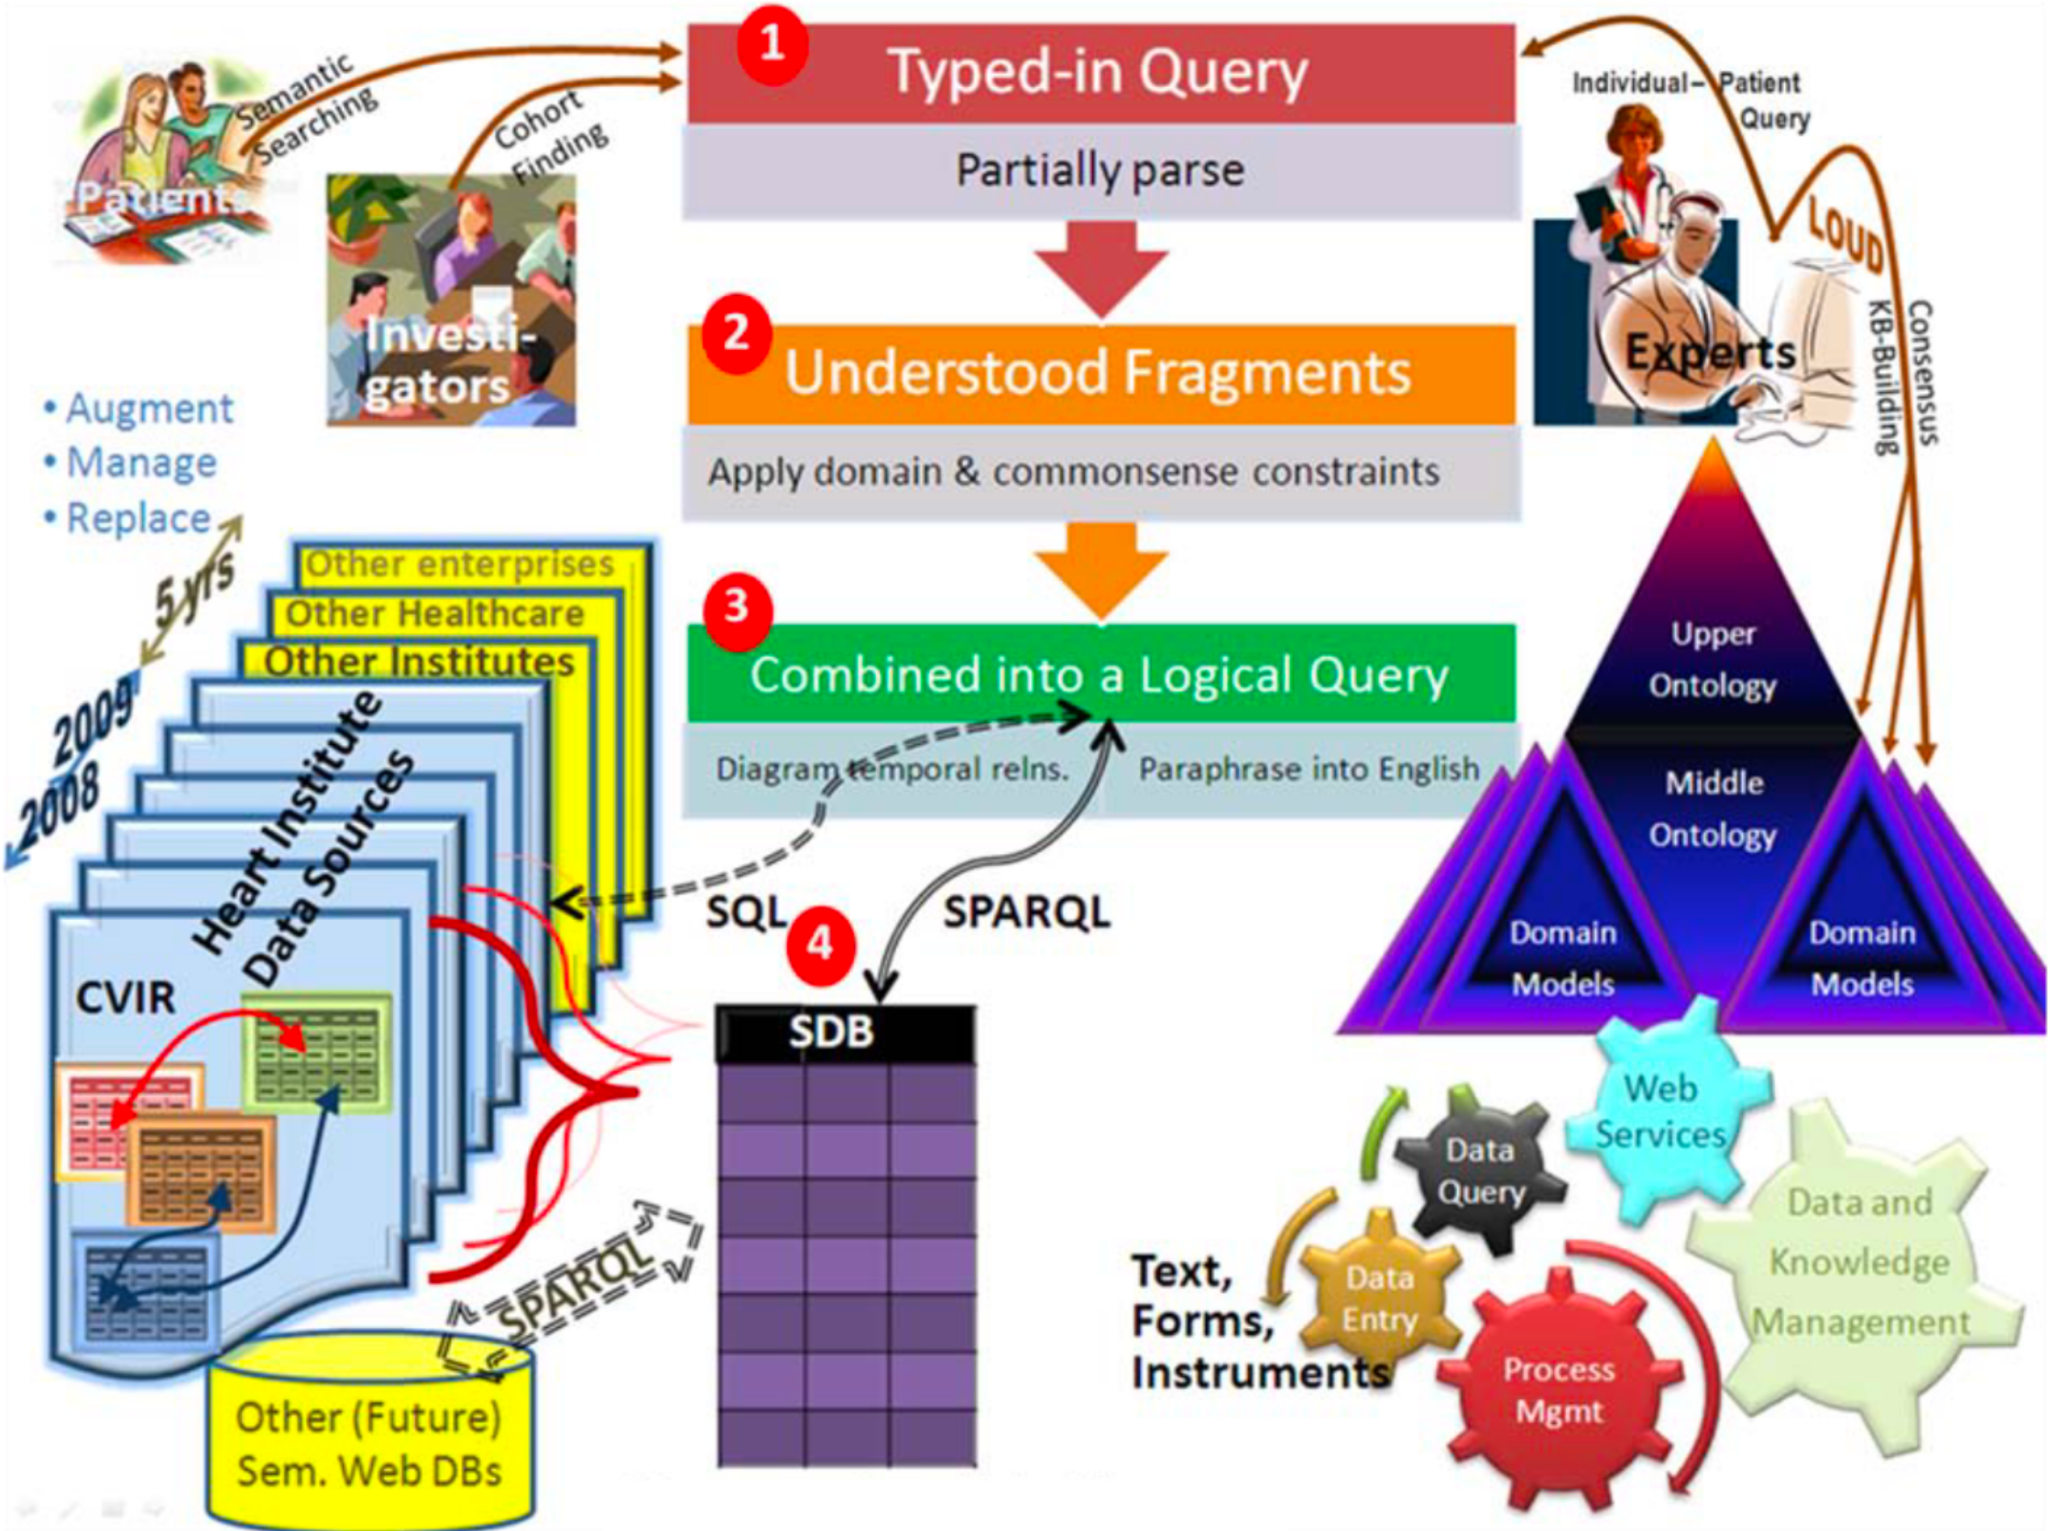
\includegraphics[width=\linewidth]{figures/f13.png}
        \caption[The Semantic Research Assistant (SRA) query-handling workflow]{\textbf{The Semantic Research Assistant (SRA) query-handling workflow} \citep[p. 7]{lenat_harnessing_2010}. Used with permission.}
        \label{fig:13}
    \end{minipage}%
    \hfill
    \begin{minipage}[t]{0.48\linewidth}
        \centering
        \includegraphics[width=\linewidth]{figures/f13r.png}
        \caption[Detail based on the Lenat et al. SRA query-handling workflow]
        {\textbf{Detail based on the Lenat et al. SRA query-handling workflow} \citep[p. 7]{lenat_harnessing_2010}.}
        \label{fig:14}
    \end{minipage}
\end{figure}
\FloatBarrier
\index[terms]{Cone Semantic Form} 


\subsection{Knowledge Translation}
I borrow the term Knowledge Translation (KT) from healthcare as a term that can be used within information as a whole, in sustainability or otherwise. In 2009, the Canadian Institutes of Health Research (CIHR) defined KT as “a dynamic and iterative process that includes the synthesis, dissemination, exchange and ethically sound application of knowledge to improve health, provide more effective health services and products and strengthen the healthcare system” \citep[p. 4]{straus_knowledge_2009-1}. 
\index[terms]{Knowledge Translation (KT)}

Climate crisis mitigation is facing overlapping challenges with health care systems when it comes to information management. In Knowledge Translation in Healthcare (2009), Straus and Tetroe report that healthcare systems are “faced with the challenge of improving the quality of care and decreasing the risk of adverse events” \citep[p. 3]{straus_knowledge_2009-1}. “Globally, health systems fail to optimally use evidence, resulting in inefficiencies and reduced quantity and quality of life” \citep[p. 3]{straus_knowledge_2009-1}. The “science and practice” of KT can help answer these challenges \citep[p. 3]{straus_knowledge_2009-1}. Similarly to the mission that drives KA in the climate crisis, closing knowledge-to-action gaps drives KT because providing evidence from research is “necessary but not sufficient for providing optimal care delivery” \citep[p. 3]{straus_knowledge_2009-1}. We might even take on the characteristics of care used in KT to further elevate the quality of human relationships we want to foster in all climate resilience KA. Knowledge Production, “distillation, and dissemination are not sufficient on their own to ensure implementation in decision making” in the “move beyond simple dissemination of knowledge to actual use of knowledge” \citep[p. 4]{straus_knowledge_2009-1}. This insufficiency is also present in climate crisis mitigation outcomes in a Sustainability Transitions Knowledge Activation (STKA).
\index[terms]{Knowledge Activation (KA)} 
\index[terms]{Knowledge Translation (KT)}
\index[terms]{Knowledge Production (KP)}
\index[terms]{climate resilience}

\subsubsection{Interdisciplinary visual methods}
\label{Interdisciplinary visual methods}

Symbolic representations of information facilitate the analysis between knowledge domains. For example, Goethe’s studies of morphology are activated into practice by Gemma Anderson-Tempini’s work. Anderson-Tempini “presents drawing as a means of developing and disseminating knowledge, and of understanding and engaging with the diversity of natural and theoretical forms, such as animal, vegetable, mineral, and four-dimensional shapes” \citep[back cover]{anderson_drawing_2018}.
\index[people]{Goethe, Johann Wolfgang von}

Anderson-Tempini defines isomorphology as “an alternative approach to classification through drawing” that “adapts Goethe’s morphological approach” \footnote{For a thorough discussion of Goethe's morphological approach see \textit{Morphology: Questions on Method and Language} \citep{molder_morphology_2013}.} to “the study of form and symmetry in whole organisms towards a focus on the parts of organisms” which “initiates a move from observation to abstraction” \citep[p. 11]{anderson_drawing_2018} \footnote{For an illustration of Anderson-Tempini’s isomorphologies see her illustration \textit{Fig 1: The primary forms and symmetries of Isomorphology} \citep{anderson_what_2013}.}. She proposes a set of “conceptual forms [...] abstracted from nature”. Specifically, she proposes thirteen “primary forms and symmetries of isomorphology” \citep{anderson_what_2013}.
\index[people]{Anderson-Tempini, Gemma}
\index[people]{Goethe, Johann Wolfgang von}
\index[terms]{isomorphology}

Anderson-Tempini’s isomorphological drawing practice is also used to represent the change over time of a given subject, ``representing morphology as a dynamic and formative process” \citep[p. 179]{anderson_drawing_2018}. This practice, called isomorphogenesis ``progresses from the empirical study of the morphology of static museum specimens towards a conceptual study that aims to draw morphology as dynamic” \citep[p. 179]{anderson_drawing_2018}. Isomorphogenesis is a ``drawing practice or `experiment'" \citep[p. 179]{anderson_drawing_2018} that captures ``four-dimensional shapes” \citep[back cover]{anderson_drawing_2018} to explore the ``potentialities of representing morphology as a dynamic and formative process”  \citep[p. 179]{anderson_drawing_2018}. Isomorphogenesis ``progresses from the empirical study of the morphology of static museum specimens towards a conceptual study that aims to draw morphology as dynamic” \citep[p. 179]{anderson_drawing_2018} \footnote{For an example of isomorphogenesis see ``Figure 15: `Isomorphogenesis’ no.10” \citep[p. 203]{anderson_drawing_2018}.}. In short, isomorphogenesis as a drawing practice illustrates the dynamic changes of a given organism over time facilitating their deeper study.
\index[people]{Anderson-Tempini, Gemma}

The impact of Anderson-Tempini’s isomorphology and isomorphogenesis practice extends internationally. This approach is formally recognized and ``has developed as a visual counterpart for the European Research Council-funded project `A process ontology for biology’, led by Professor John Dupré at the University of Exeter” \citep[p. 179]{anderson_drawing_2018}. Anderson-Tempini’s isomorphology and isomorphogenesis methods contribute substantially to classifying natural forms and visualizing their dynamic traits and transformations through drawing.
\index[people]{Anderson-Tempini, Gemma}
\index[terms]{isomorphology}

\subsection{Knowledge Production}
To recap, KSSTP stands for Knowledge Surfacing, Synthesis, Translation, and Production. This section, Knowledge Production, concludes the literature review section dedicated to defining the terms and dynamics involved in KSSTP.
\subsubsection{Induction, deduction, and abduction in Peirce}
Within KSSTP, Sowa’s understanding of Peircean analogy is closer to what I mean by Knowledge Surfacing; Adler’s ``syntopical reading” and Wilson’s consilience are closer to what I mean by Knowledge Synthesis. Peircean abduction is closer to what I mean by Knowledge Production because it is about proposing something new. In fact, Peirce defines abduction as ``the process of forming an explanatory hypothesis”, the “only logical operation which introduces any new idea”, and the only means to ``learn anything or to understand phenomena at all"  \citep[p. 106]{peirce_pragmatism_1960}. 
\index[terms]{abduction}
\index[people]{Peirce, Charles Sanders}
\index[people]{Sowa, John F.}
\index[people]{Adler, Mortimer J.}
\index[people]{Wilson, Edward O.}
\index[terms]{syntopical reading}
\index[terms]{Knowledge Surfacing (KSu)}
\index[terms]{Knowledge Synthesis (KSy)}
\index[terms]{Knowledge Production (KP)}
\index[terms]{consilience}
\index[terms]{analogy} 

Peirce elaborates that induction ``does nothing but determine a value"  and ``shows that something actually is operative"; deduction ``merely evolves the necessary consequences of a pure hypothesis" and ``proves that something must be"; abduction ``merely suggests that something may be", and ``Its only justification is that from its suggestion deduction can draw a prediction which can be tested by induction" \citep[p. 106]{peirce_pragmatism_1960}. In the case of the title of this thesis, it is the \textit{may} in the \textit{What may be known}. 
\index[people]{Peirce, Charles Sanders}
\index[terms]{abduction}


The mystery of introducing ``any new idea” \citep[p. 106]{peirce_pragmatism_1960} is captured by Peirce when he wrote: ``No reason whatsoever can be given for it, as far as I can discover; and it needs no reason, since it merely offers suggestions” \citep[p. 106]{peirce_pragmatism_1960}. It would seem that curiously that the illusive Knowledge Production is vital to moving any theory forward, and yet its abduction ``needs no reason” and constitutes only a proposal for the direction of further study, relying on the other forms of logical operation to constitute if it ``may be” or ``must be” \citep[p. 106]{peirce_pragmatism_1960}.
\index[people]{Peirce, Charles Sanders}
\index[terms]{abduction}
\index[terms]{Knowledge Production (KP)}


Wilson’s borderland disciplines \citep[p. 12]{wilson_consilience_1999} and Adler’s \textit{Syntopicon} can work together in syntopical consilience as a means towards creating ``new language” \citep[p. 185]{pangaro_design_2011}. Syntopical consilience offers the possibility of Peircean abduction or introducing a ``new idea” \citep[p. 106]{peirce_collected_1960}. Therefore, I propose that in KSSTP, the confluence of Knowledge Synthesis, Knowledge Translation, and Knowledge Production can be referred to as Syntopical Consilient Abduction.
\index[terms]{abduction}
\index[people]{Pangaro, Paul} 
\index[people]{Peirce, Charles Sanders}
\index[people]{Adler, Mortimer J.}
\index[terms]{Syntopicon}
\index[terms]{Knowledge Translation (KT)}
\index[terms]{Knowledge Production (KP)}
\index[terms]{consilience}
\index[terms]{syntopical consilience}


\section{Design across KSSTP}
\noindent Design works across the various forms of KSSTP, surfacing, synthesizing, translating, and creating: surfacing by revealing relationships between ideas in techniques like topic modelling, synthesizing by combining ideas in techniques like Systematic Combining \citep[p. 554]{dubois_systematic_2002}, translating by framing ideas from one discipline in the ways that another can receive and understand \citep[p. 3]{straus_knowledge_2009-1} and creating in generative methods like gigamapping \citep{sevaldson_giga-mapping_2011}. In this section, we will cover various forms of design that relate to KSSTP within discussions of composition, spatial composition, visual forms of Knowledge Production, information design, Systems Oriented Design, Systematic Combining, Design for Sustainability Transitions, and the torus as an isomorph for visual reasoning.
\index[people]{Sevaldson, Birger} 
\index[terms]{gigamapping}
\index[terms]{Systematic Combining (SC)}
\index[people]{Gadde, Lars-Erik}
\index[people]{Dubois, Anna}
\index[terms]{torus}
\index[terms]{Knowledge Surfacing (KSu)}
\index[terms]{Knowledge Production (KP)}
\index[terms]{Systems Oriented Design (SOD)}

To ``distinguish design from Design”, Sevaldson notes that B. Archer “made a distinction between design and Design with a capital D [...]. Design with a Capital D is a third area of knowledge and education equal to science and the humanities, with relations to arts and technology” \citep[p. 91]{sevaldson_designing_2022}. In Archer’s own words: ``Design, in its most general educational sense, where it is equated with Science and the Humanities, is defined as the area of human experience, skill and understanding that reflects man’s concern with the appreciation and adaptation of his surroundings in the light of his material and spiritual needs. In particular, though not exclusively, it relates with the configuration, composition, meaning, value and purpose in man-made phenomena” \citep[p. 20]{archer_design_1979}. Archer, as cited by Sevaldson, thus posits Design as a distinct knowledge domain alongside science and the humanities.
\index[people]{Sevaldson, Birger}

Sevaldson entreats: ``It is urgent to develop and reinforce this perspective of Design as an equal area to science and the humanities. Design should be viewed as a unique mode of knowledge production that can be used to achieve the systemic changes needed for future systemic innovations” \citep[p. 91]{sevaldson_designing_2022}. Furthermore, Sevaldson articulates: ``Design is inherently systemic. Any design must relate to users, production methods, culture, aesthetics, business economy, and technology. In that sense, it is always a result of negotiation and navigation within networks of relations between large complex systems. Without putting in the effort to understand, to the best of our abilities, these networks of relations, one will not be able to produce design outs that function well in the world” \citep[p. 91]{sevaldson_designing_2022}. Sevaldson posits Design as a systemic knowledge domain crucial for innovation and navigating complex interdisciplinary relational networks.
\index[people]{Sevaldson, Birger}
\index[terms]{Knowledge Production (KP)}

Epistemologically, I posit that Archer's Design, as opposed to lowercase-d design, is a semantic field for Wilson's consilience, in which it is possible to further integrate Science and the Humanities.
\index[people]{Wilson, Edward O.}
\index[terms]{consilience}


\subsection{Composition}
To define the composition, we must first consider what it means to be `whole.’ At first glance, the famous aphorism ``The whole is greater than the sum of the parts” captures the core of Gestalt psychology. This statement is often attributed to Aristotle, or to Systems Thinking \citep[p. 164]{sevaldson_designing_2022}\footnote{For a more fulsome retracing of the lineage of thinkers that lead to Systems Thinking as a practice, see ``History and State of Systems Thinking in Design” in Sevaldson (2022), p. 149-150 \citep[p. 148-150]{sevaldson_designing_2022}.}, but it merits clarification. To cite Gestalt psychologist Kurt Koffka in Sevaldson, ``The whole is other than the sum of its parts” \citep[p. 164]{sevaldson_designing_2022}\footnote{For a more fulsome connection between Gestalt and design and systems see ``Gestalt Psychology” in Sevaldson (2022), p. 186-188 \citep[p. 163-167]{sevaldson_designing_2022}.}. Koffka’s statement is closer to the words of Aristotle, who wrote ``the whole is something beside the parts” \citep{aristotle_metaphysics_1989}. To treat with composition, we need to recognize the ways wholes have properties distinct from their parts' properties.
\index[people]{Sevaldson, Birger}

Composition, or the interpretation of wholes and parts, is fundamental to understanding. Noam Chomsky argues that composition is foundational to language \citep{chomsky_knowledge_1986,chomsky_syntactic_2002}, Sevaldson suggests that it is ``the most important notion of design” \citep[p. 162]{sevaldson_designing_2022}, and Geman et al. argue it is “fundamental to all of cognition” \citep[p. 1]{geman_composition_2002}. Furthermore, Geman et al. define composition the semantics engaged in composition as the ability ``to represent entities as hierarchies of parts, with these parts themselves being meaningful entities, and being reusable in a near-infinite assortment of meaningful combinations” \citep[p. 1]{geman_composition_2002}. As Sevaldson puts it: ``Composition in design can be understood as a special way of synthesis in shape and form. In art, composition rests on its own objective, and creates its own logic” \citep[p. 167]{sevaldson_designing_2022}. Composition (i.e., the way we combine and interpret parts to create a whole) is fundamental to understanding language, design, and cognition.
\index[people]{Sevaldson, Birger}
\index[terms]{composition}

In the converse of \textit{composition}, Sevaldson offers additional subtlety to the discussion of \textit{decomposition}. Sevaldson writes object-oriented approaches offer less emphasis on the relation between entities, which ``comes as a natural consequence of their reference to language, where the relation between the words (entities) is proximal rather than a potential process or signal by its own right” \citep[p. 169]{sevaldson_designing_2022}. In this thesis, I adopt an approach closer to Sevaldson’s, where the relation between entities in composition is itself a signal that carries its own meaning.
\index[people]{Sevaldson, Birger}
\index[terms]{composition}


\subsection{Spatial composition}
Further to visual experience in space, treatments of spatial composition exist. In Semiotics of \textit{visual language} (1990), Saint-Martin introduces a syntax of sculptural language and its laws, including topological relations, by using the infrastructure of the virtual cube as corresponding ``to the contour of the most unified geometrical forms”, and having ``preeminent status in the perceptual process” \citep[p. 173-174]{saint-martin_semiotics_1990}. Proposing to work within the gestaltian cube continues to be a distinctly Euclidean perspective. While I appreciate that the constraints of point-plotting within the cube can provide a starting point, other methods of plotting points and examining their relationships exist, such as the embedding into spherical space, hyperbolic space, and custom metric space \citep{mcinnes_embedding_2018}.
\index[people]{Saint-Martin, Fernande}
\index[terms]{composition}

Saint-Martin, however, goes on to distinguish the types of mathematics used to understand meaning-making in three-dimensional space. She recalls that in ``the 1940s, the genetic epistemology of Piaget established that the first geometrical model of space used by human beings is not Euclidian geometry but topology. This spatial model of the organization of perceptual experience remains throughout human life the basic means by which one constructs his notions of reality” \citep[p. 68]{saint-martin_semiotics_1990}. 
\index[people]{Saint-Martin, Fernande}
\index[terms]{topology}

Saint-Martin and Johanna Drucker, author of \textit{Graphesis} (2014), imagine futures with integration of topological semantic expression. In The Semiotics of Visual Language Saint-Martin writes that she is ``entrusting to a future work the development of the semantic system of topological semiotics” \citep[p. 225]{saint-martin_semiotics_1990}  Drucker proposes that topological concepts could be useful in analyzing “textual structures” and ``paratextual apparatuses”, including marginal notes, footnotes, and layout features \citep[p. 54]{drucker_graphesis_2014}. She emphasizes that understanding continuity and discontinuity in text interpretation is crucial for interpreting hyperlinked environments \citep[p. 54]{drucker_graphesis_2014}. However, Drucker notes that we still need to develop a specialized `metalanguage’ to describe how graphical elements convey relationships in digital spaces and how they contribute to the text's meaning through their ``structuring effects” \citep[p. 54]{drucker_graphesis_2014}. Drucker poignantly muses with the imagery of space: ``Thought forms expressed in the constellationary field may be abstracted and studied for their configuration of knowledge as well as their content, and the organizing orders of graphical expression will take on their own legibility” \citep[p. 196]{drucker_graphesis_2014}. Saint-Martin and Drucker envision a future where topological concepts are integrated into semantic and textual analysis, emphasizing the need for a new language to interpret graphical relationships in digital spaces.
\subsection{Visual Forms of Knowledge Production}
Johanna Drucker might categorize the diagrams which Tversky sees as a ``platform for inference” as ``visual forms of knowledge production” \citep{drucker_graphesis_2014} distinct from visual forms of information display. In fact, Drucker defines graphesis as ``the study of the visual production of knowledge” \citep[p. 3]{drucker_graphesis_2014}.
\index[people]{Drucker, Johanna}
\index[people]{Tversky, Barbara}
\index[people]{Saint-Martin, Fernande}

More widely than diagrams and interface, Drucker’s work offers much-needed clarity in visual epistemology, or ``ways of knowing that are presented and processed visually” \citep[p. 8]{drucker_graphesis_2014}. She underscores the epistemological urgency of this thesis when she writes: ``Visual expressions of knowledge are integral to many disciplines in the natural sciences, but language-oriented humanities traditions have only barely engaged with visual forms of knowledge” \citep[p. 7]{drucker_graphesis_2014}. Drucker’s insights in visual epistemology extend beyond diagrams and interfaces to include \textit{visual arguments}. Tversky found that when it comes to visual arguments and visual reasoning as a whole, ``well-crafted diagrams are superior to language for explaining many kinds of information—more directly, more succinctly” \citep{tversky_barbara_2022}. Furthermore, visual explanations are ``a check for coherence, a check for completeness, and a platform for inference” \citep{tversky_barbara_2022}. In other words, well-made graphs are worth more than a thousand words, specifically because they can act as visual arguments and help us reason through complex information in ways that are more effective than using only words. 
\index[people]{Drucker, Johanna}
\index[people]{Tversky, Barbara}

Drucker argues that information visualizations often present themselves as objective representations of data when, in fact, they are interpretative arguments made through visual means \citep[p. 10]{drucker_graphesis_2014}. Drucker points out the paradox of how visual forms of knowledge production across various media tend to conceal the visual ways arguments get constructed \citep[p. 10]{drucker_graphesis_2014}. Drucker’s book aims to highlight these visual forms of knowledge production and develop a critical framework for analyzing them. 
\index[people]{Drucker, Johanna}

\subsubsection{Graphical User Interface (GUI)}
%\noindent \textbf{GUI} \\
In a historical context when ``we carry on most of our personal and professional business through interfaces”, it is pertinent to single out that ``no single innovation has transformed communication as radically in the last half century as the GUI”, the Graphical User Interface \citep[p. 8]{drucker_graphesis_2014}. The importance of the GUI is in no small part because of its graphesis. 
\index[people]{Drucker, Johanna}

Drucker encouragingly describes the simultaneously technical and interpretative endeavour of graphesis as a view ``into the studio laboratory of knowledge design, where we sit at the consoles of workstations meant to help engineer and imagine the creation and implementation of a diagrammatic and constellationary rhetoric, of writing in the infinitely extensible field populated by new conventions of legibility that structure and organize expression and communication” \citep[p. 197]{drucker_graphesis_2014}. Drucker then adds that ``the workstation dissolves into infinite play of text and task, knowledge as performance and invention, a cognitive engine engaged with the collective life of embodied mind” \citep[p. 197]{drucker_graphesis_2014}. Drucker’s description of the studio laboratory of knowledge design is a more humanistic facet of the more computer-science-oriented approach called knowledge engineering, or the use and construction of a computational knowledge-based system used for problem-solving \citep[p. 8]{wielinga_kads_1992}. Drucker’s sense of graphesis as a technical and interpretative endeavour sets the stage for a more humanistic approach to knowledge design.
\index[people]{Drucker, Johanna}
%``Cognitive engine" \citep[p. 197]{drucker_graphesis_2014}.
 
The ``subjective display of humanistic phenomena can be applied across” domains in the following ``four basic levels” of ``visualizing interpretation” \citep[p. 135]{ drucker_graphesis_2014} or ``visual forms knowledge production” \citep{drucker_graphesis_2014}: 
“1) Modeling phenomenological experience in the making of humanities (\textit{data} as \textit{capta}, primary modeling, the representation of temporal and spatial experience); 
2) Modeling relations among humanities documents, i.e., discourse fields (a different metric might be needed to understand dates on diplomatic documents from the spring of 1944 or 1950); 
3) Modeling the representations of temporality and spatiality that are found in humanities documents (narrative is the most obvious); 
4) Modeling the interpretation of any of the above (depicting or graphing the performative quality of interpretation)” \citep[p. 135]{ drucker_graphesis_2014}. 
\index[people]{Drucker, Johanna}
\index[terms]{capta}

\subsubsection{Humanistic Design}
The ``humanist commitment to interpretation”, ``embracing ambiguity […,] contradictions and the lack of fixity or singularity”, and the ways that “forms of classification, taxonomy, or information organization embody ideology” \citep[p. 178]{drucker_graphesis_2014} are not mutually exclusive to the value of synthesis across ideology and taxonomy. Wilson’s borderland disciplines and Adler’s \textit{Syntopicon} are evidence of how ambiguity can coexist and even benefit from the synthetic “fixity” (i.e., artificial stability) of consilience and syntopical reading, ideological or otherwise. In fact, Drucker later revisits this comingling of “fixity” and ambiguity in the afterword of \textit{Graphesis}: “The interpretative and the empirical need not exclude each other. So the graphic grammar of an emerging visual system inclined to present the embodied, situated, circumstantial, and fragmentary quality of knowledge will embrace specificities and particularities even as it makes possible the social mediation of communicative exchange” \citep[p. 196]{drucker_graphesis_2014}.
\index[people]{Drucker, Johanna}
\index[people]{Adler, Mortimer J.}
\index[people]{Wilson, Edward O.}
\index[terms]{Syntopicon}
\index[terms]{syntopical reading}
\index[terms]{consilience}

Drucker’s \textit{Graphesis} captures an ontological ethos for humanistic information design in which she advocates for advancing beyond the terms “set by disciplines whose fundamental beliefs are antithetical to interpretation” \citep[p. 178]{drucker_graphesis_2014}. In her vision of critical design for interpretative and humanistic interfaces, Drucker emphasizes the importance of revealing the constructedness of knowledge and facilitating interpretative activity with tolerance for “inconsistency among types of knowledge representation, classification, fluid ontologies, and navigation” \citep[p. 178]{drucker_graphesis_2014}. Drucker’s work lays the foundation for the evolution of scholarly tools toward more dynamic, relational, and interpretative approaches in humanistic information design.
\index[people]{Drucker, Johanna}

Drucker argues that we “are in the incunabula of information design” \citep[p. 176]{drucker_graphesis_2014}. She identifies emerging “new conventions that do not rely on book structures” \citep[p. 176]{drucker_graphesis_2014} in information software. Drucker emphasizes that the “new condition for scholarly activity is relational and dynamic”, prioritizing process over product \citep[p. 176]{drucker_graphesis_2014}. She notes that ``Informational derivatives of data mining, analytics, visualization, and display are increasingly a part of a reading environment in scholarly, political, and business activity” to visualize “these networked relations, communities of scholarly exchange, argument, comment, linked references, framings, and embedded citations” \citep[p. 176]{drucker_graphesis_2014}. Drucker advocates for “an interface that is meant to expose and support the activity of interpretation, rather than to display finished forms” \citep[p. 179]{drucker_graphesis_2014}, representing a shift towards praxis in humanistic information design. Drucker envisions the dawn of humanistic information design as emphasizing dynamic and interpretative interfaces that visualize networked scholarly discourse and prioritize process over finished products.
\subsection{Information visualization and information design }
Drucker defines information graphics and information visualization as “visualizations based on abstractions of statistical data”, or “metrics expressed as graphics” \citep[p. 7]{drucker_graphesis_2014}. Sevaldson writes that information visualizations make information “accessible and understandable” \citep[p. 186]{sevaldson_designing_2022}. The impact of information visualization has been great, ``and in many cases, the visual serves as scientific (ostensive) proof” \citep[p. 186]{sevaldson_designing_2022}. Information visualization is a valuable practice for displaying the various modes of Knowledge Activation. 
\index[people]{Drucker, Johanna}

Data “does not have an inherent visual form”, so visualizations are also necessarily interpretations \citep[p. 7]{drucker_graphesis_2014}. Information visualization “creates a bridge between sciences and the arts. It is often aesthetic decisions that influence the interpretation of the visualisations” \citep[p. 186]{sevaldson_designing_2022}. The interpretativeness of information visualizations, and data representations more generally, are a means of bridging art and science through aesthetic decisions that shape them.
\index[people]{Drucker, Johanna}

However, the limitation of information visualization is that it is “with very few exemptions, descriptive”, and often this happens through “simplification and reduction of the complexity of the material” \citep[p. 186]{sevaldson_designing_2022}.
\index[people]{Sevaldson, Birger}


\subsection{Systems Oriented Design (SOD)}
The complexity of science and design research as a field of Knowledge Production ``demands an equally rich repertoire of interrelated methods and positions” \citep[p. 8]{sevaldson_discussions_2010-1}. 
\index[people]{Sevaldson, Birger}
\index[terms]{Knowledge Production (KP)}
\index[terms]{Systems Oriented Design (SOD)}

As introduced earlier, one such codified repertoire is Systems-Oriented Design (SOD), an interdisciplinary methodology that combines systems thinking with design practice to tackle super-complex multi-level problems by integrating diverse information in generative rather than descriptive means \citep[p. 27, p. 152, p. 157]{sevaldson_designing_2022}. SOD is a “dialect” in the larger field called Systemic Design which is distinguished by its inclination towards design practice. SOD is also sometimes called the Oslo-School of Systemic Design \citep[p. 2]{sevaldson_designing_2022}\footnote{For a more fulsome retracing of how Systemic Design emerged as a field see “Systemic Design: The Renaissance of Systems Thinking in Design” \citep[p. 186-188]{sevaldson_designing_2022}.}.
\index[terms]{Systemic Design}
\index[people]{Sevaldson, Birger}

Central to SOD is the practice of gigamapping, a technique for visually representing complex systems and their interconnections \citep[p. 26]{sevaldson_designing_2022}. Notably, gigamapping avoids hierarchy and orients practitioners to investigate relationships and meta-relationships like unknown unknowns \citep[p. 55, p. 353-357]{sevaldson_designing_2022}. These principles speak to the utility of gigampping as a post-structuralist tool for the definition of systems and ideas. SOD integrates constructivist learning in a way that emphasizes the designer's role in shaping systems through continuous exploration, intervention, and adaptation \citep[p. 153]{sevaldson_designing_2022} \footnote{For a retracing of constructivist learning theory, Sevaldson notes that it has been influenced by Lev Vygotsky, Herbert Simon, Heinz von Foerster, and Humberto Maturana \citep[p. 153]{sevaldson_designing_2022}.}
\index[people]{Sevaldson, Birger}
\index[terms]{gigamapping}

In Sevaldson, we find an example of how the network graph provides a distinctly useful medium for managing the discussed epistemological ambiguity in a versatile, decentralized, interdisciplinary representation of entities and relationships, namely, Christopher Warnow's \textit{Map of Systems Theory} (2012) \citetext{\citealp[p. 125]{sevaldson_designing_2022}; \citealp{warnow_map_2012}}. 
\index[people]{Sevaldson, Birger}

Systems Oriented Design encourages systemic designers to understand the dynamics of systems and intervene at various levels while considering the ethics, ripple effects, and consequences of their work \citep[p. 95-96]{sevaldson_designing_2022}. This includes “evaluating and re-evaluating the constructed boundary when working with a system” \citep[p. 146]{sevaldson_designing_2022}, or boundary critique \citep{midgley_theory_1998}.
\index[terms]{Systemic Design}
\index[people]{Sevaldson, Birger}
\index[terms]{Systems Oriented Design (SOD)}

Here at OCAD University, Peter Jones compiled the practice of synthesis mapping based on Sevaldson’s gigamap method \citep[p. 129]{jones_synthesis_2017} in and through the Strategic Innovation Lab (sLab). Jones, Shakdher and Singh used the synthesis map method in the Knowledge Translation of Healthcare Systems \citep[p. 129]{jones_synthesis_2017}. 
\index[terms]{gigamapping}
\index[terms]{Knowledge Translation (KT)}
 \clearpage

 \FloatBarrier
\begin{figure}[h]
    \centering
    \includegraphics[width=0.6\linewidth]{figures/f15.png}
    \caption[Diagram of the SOD Creative Process Framework]
    {\textbf{Diagram of the SOD Creative Process Framework} \citep[p. 312]{sevaldson_designing_2022}. Used with Sevaldson's permission.}
    \label{fig:15}
\end{figure}

\begin{figure}[h]
    \centering
    \includegraphics[width=0.6\linewidth]{figures/f18.png}
    \caption[Diagram of a design process with iterations]{\textbf{Diagram of a design process with iterations} \citetext{\citealp[p. 343]{sevaldson_designing_2022}; \citealp{sevaldson_designing_2022-1}}. Used with Sevaldson's permission.}
    \label{fig:18}
\end{figure}
\FloatBarrier

\FloatBarrier
\begin{figure}[h]
    \centering
    \includegraphics[width=0.6\linewidth]{figures/f16.png}
    \caption[An example gigamap]
    {\textbf{An example gigamap}. Making Waves: Organizational gigamap by Angel L. Lamar Oliveras \citep{lamar_oliveras_making_2020}. Used with permission under the CC-BY-NC-ND 4.0 International License.}
    \label{fig:16}
\end{figure}
\index[terms]{gigamapping}

\begin{figure}[h]
    \centering
    \includegraphics[width=0.6\linewidth]{figures/f17.png}
    \caption[Key to example gigamap]
    { \textbf{Key to example gigamap} \citep{lamar_oliveras_making_2020}. 
Used with permission under the CC-BY-NC-ND 4.0 International License.}
    \label{fig:17}
\end{figure}
\FloatBarrier

\subsection{Systematic Combining (SC)}
If climate is everyone’s problem, and climate is a system of systems, then systems approaches are everyone’s problem, including designers. Robust Systemic Design approaches to sustainability are emerging, like the recent work of Svein Gunnar Kjøde, a student of Birger Sevaldson.
\index[terms]{Systemic Design} 
\index[terms]{Systematic Combining (SC)}

The systems approach to research called Systematic Combining (SC) is the central strategy for Kjøde’s Entanglement of Systemic Design and Sustainability Transitions (2024). Dubois and Gadde proposed the term “systematic combining” in 2002 and described it as “a process where theoretical framework, empirical fieldwork, and case analysis evolve simultaneously, and it is particularly useful for development of new theories” \citep[p. 554]{dubois_systematic_2002}. They note that the “main characteristic of this approach is a continuous movement between an empirical world and a model world” \citep[p. 554]{dubois_systematic_2002} “grounded in an ‘abductive’ logic” \citep[p. 553]{dubois_systematic_2002}. Systematic Combining offers a dynamic approach to theory development through the simultaneous evolution of framework, fieldwork, and analysis. The application of SC in sustainability transitions research highlights its ability to handle complex, interconnected, and emergent phenomena.
\index[terms]{abduction}
\index[terms]{Systemic Design}
\index[terms]{Systematic Combining (SC)}
\index[people]{Gadde, Lars-Erik}
\index[people]{Dubois, Anna}


Systematic combining de-emphasizes data verification and accuracy. Instead, it leverages how “multiple sources may contribute to revealing aspects unknown to the researcher, i.e., to discover new dimensions of the research problem” \citep[p. 556]{dubois_systematic_2002}. “As such,” Kjøde explains, “the approach arguably supports an investigation that navigates rapidly developing, interdisciplinary fields of knowledge that not only study the systemic phenomena of sustainability transitions but becomes a system of dynamic knowledge in itself” \citep[p. 46]{kjode_entanglement_2024}. According to Sevaldson and Kjøde, systems-oriented design inquiry methods must be able to handle interrelation and contradiction of ideas \citetext{\citealp[p. 46]{kjode_entanglement_2024}; \citealp[p. 8]{sevaldson_discussions_2010-1}}. Kjøde writes that his choice to use SC in his doctoral work “responds directly to the complex, interconnected and emergent nature of the sustainability transitions field” \citep[p. 45]{kjode_entanglement_2024}. Systematic Combining prioritizes discovering new research dimensions through multiple sources, making it well-suited for complex interdisciplinary fields like climate crisis KA, which requires handling interrelated, evolving, and contradictory ideas.
\index[people]{Kjøde, Svein Gunnar}
\index[terms]{Systematic Combining (SC)}
\index[people]{Gadde, Lars-Erik}
\index[people]{Dubois, Anna}


\subsection{Design for Sustainability Transitions (DfST)}
 Grin et al. define Sustainability Transitions (ST) as “radical transformation towards a sustainable society” \citep[p. 1]{grin_introduction_2011} involving an axiological “quest for new value systems” \citep[p. 2]{grin_introduction_2011}, “a shift to a more sustainable economy” \citep[p. 1]{grin_introduction_2011}, and “long-term and complex socio-technical transitions” \citep[p. 11]{geels_introduction_2011}. Design for Sustainability Transitions (DfST), also called Transition Design, is a “kind of designing that is connected to long horizons of time and visions of sustainable futures” \citep[p. 3]{irwin_transition_2015}. In short, sustainability-oriented multi-systemic interdisciplinary information processes and their societal outcomes are supported by Design for Sustainability Transitions. 

Flittner et al. (2022) elaborate that DfST combines frameworks and methods from a variety of fields, like transition management, anthropology, design research, and sustainability science, towards a practice for building enduring “transitions towards more sustainable societies” \citep[p. 160]{flittner_design_2022}. ST and DfST are both, then, interdisciplinary, longitudinal, iterative, multi-praxis, multi-systemic, cross-sectoral theoretical work which sustains the potential for “complementary understandings” \citep[p. 197]{oztekin_co-positioning_2020} and operationalization of social change. Furthermore, DfST engages three embedded levels of Systemic Design complexity described by Robert Young: (a) ``design in context" or ``design at the level of products and artefacts”, (b) ``designing context” or ``design at the level of systems and services”, and (c) ``design of context” or ``design at the level of policy, ideology, purposes, values and norms” \citep[p. 200]{oztekin_co-positioning_2020}.

All design must take into account ST, and in some sense, all responsible design is DfST. As such, this thesis works towards ST through KA, or STKA for short.
\index[terms]{Systemic Design}

\subsection{The torus}

\subsubsection{Torus isomorph as a composition for visual reasoning}
The torus, with its captivating visual and mathematical properties, emerges as an isomorph in diverse disciplines and contexts. My initial encounter with the torus was through interpretations of chakra geometry whereby tori are used to represent cyclical energy fields in and around the human body \citep{singer_quantum_2019}.
\index[terms]{torus}
\index[terms]{composition}

In \textit{Rudy Rucker's Infinity and the Mind (2005)}, the torus is employed to model space-time, depicting an oscillating universe with circular time. Rucker's toroidal model suggests a universe where time loops back onto itself in a continuous cycle as shown in \autoref{fig:19}. In 2013, the Resonance Science Foundation (RSF) produced an animation of the yin yang mapped onto a torus. This work is an example of how paradoxes of the cosmological imagination can be visuospatialized using the torus
\citep{resonance_science_foundation_yin_2013}.

\index[people]{Rucker, Rudy}
\index[terms]{torus}

As I directed my research away from cosmology in this thesis, I continued to encounter the torus in a surprising variety of fields in ways that captured a variety of phenomena. For example, Gardner et al. use TDA of the recordings of hundreds of rat grid cells to demonstrate that ``the joint activity of grid cells from an individual module resides on a toroidal manifold" \citep[p. 123]{gardner_toroidal_2022}, as shown in \autoref{fig:20}. Furthermore, positions ``on the torus correspond to positions of the moving animal in the environment" \citep[p. 123]{gardner_toroidal_2022}. 
\index[terms]{torus}
\index[terms]{Topological Data Analysis (TDA)}

To better understand the tori I encountered, I turned to a mathematical classification of tori \citep{weisstein_torus_nodate}, which identifies three distinct types as shown in \autoref{fig:21}: horn torus, ring torus, and spindle torus. 
\index[terms]{torus}
\index[terms]{horn torus}

My journey with the torus led me to the potential of plotting text graphs using toroidal composition. The wide range of disciplines the torus already emerges in is compelling evidence for its application in more ways. Starting points for direct application include toroidal isomorphs, representation of complex feedback loops. 
\index[terms]{torus}
\index[terms]{topology}

In the context of the climate crisis and the urgent need for consilient, syntopical information practices, the torus presents a valuable tool. Integrating insights from Tversky's work on the neuroscience of visuospatial reasoning, Anderson-Tempini's concepts of isomorphology and isomorphogenesis, and Drucker's approaches to visual Knowledge Production, the torus can facilitate new methods of data visualization and understanding.
\index[people]{Drucker, Johanna}
\index[people]{Tversky, Barbara}
\index[people]{Anderson-Tempini, Gemma}
\index[terms]{torus}
\index[terms]{Knowledge Production (KP)}
\index[terms]{isomorphology}

Advancements in three-dimensional information plotting enable the production of dynamic toroidal models, particularly through platforms like UMAP \citep{mcinnes_embedding_2018}, Python, Blender and others. Combined with hyperlinked bibliometric interfaces such as Obsidian and Litmaps, these tools support the activation and navigation of large textual datasets using visuospatial graphing, which is crucial in addressing the complexities of the climate crisis.

By investigating the isomorphic properties of the torus, we can leverage its distinct interdisciplinary presence to develop innovative ways to represent and analyze interconnected systems. For example, as a metaphorical and practical framework for systemic thinking, toroidal topology embodies the cyclical and recursive nature of knowledge transformation.
\index[terms]{torus}
\index[terms]{topology}
\index[terms]{Blender (software)}

In short, toroidal versatility in isomorphology, geometry, and topology can be used to bridge academic fields in STKA. 
\index[terms]{torus}

\FloatBarrier
\begin{figure}[h]
    \centering
    \includegraphics[width=0.5\linewidth]{figures/f19.png}
    \caption[Rucker horn torus model representing ``an oscillating universe with circular time”]
    {\textbf{Rucker horn torus model representing ``an oscillating universe with circular time”} \citep{rucker_infinity_2005}. Used with Rucker's permission.}
    \label{fig:19}
\end{figure}
\index[terms]{torus}
\index[terms]{horn torus}

\begin{figure}[h]
    \centering
    \includegraphics[width=0.5\linewidth]{figures/f20.png}
    \caption[Illustration of ``signatures of toroidal structure in the activity of a module of grid cells”]
    {\textbf{Illustration of ``signatures of toroidal structure in the activity of a module of grid cells”} \citep[p. 124]{gardner_toroidal_2022}. Used with permission.}
    \label{fig:20}
\end{figure}

\begin{figure}[h]
    \centering
    \includegraphics[width=0.5\linewidth]{figures/f21.png}
    \caption[The three standard tori]
    {\textbf{The three standard tori} \citep{weisstein_torus_nodate}. This illustration shows the three types of tori: ring torus, horn torus, and spindle torus. Each type is shown as a full view, cutaway, and cross-section through the z-axis. Used with permission.}
    \label{fig:21}
\end{figure}
\FloatBarrier
\index[terms]{torus}
\index[terms]{horn torus}
\index[terms]{ring torus}


\subsubsection{Torus anatomy}

To better prepare the reader for my later discussions of the ring torus and the horn torus, I offer a short primer on the anatomy of the torus. The distance from the centre of the torus to the centre of the torus's body, also called the torus tube, is the Major Radius (R). The radius of the tube itself is the Minor Radius (r), measured from the tube's centre to its outer surface. The Major Diameter (D or 2R) is the distance between torus centre lines. The Minor Diameter (d or 2r) is the diameter of the torus tube. The Outer Diameter is the total width of the torus at its widest and is equal to the sum of the Major Diameter (D) and the Minor Diameter (d) (D+d). The Inner Diameter of the torus is the diameter of the torus hole, and it is equal to subtracting the Minor Diameter from the Major Diameter (D-d). 
\index[terms]{torus}
\index[terms]{horn torus}
\index[terms]{ring torus}

\FloatBarrier
In \autoref{f4.1.tori anatomy}, I illustrate a top view of the two tori from \autoref{fig:21} most relevant to this thesis, the ring torus and the horn torus. Note that the horn torus pinches to a single point, while the ring torus has an opening in its doughnut-like form. This key difference means that the horn torus is illustrated with no Inner Diameter, Major and Minor Radii of equal length, Major and Minor Diameters also of equal length, and no change to the Major Diameter.  

\index[terms]{torus}
\index[terms]{horn torus}
\index[terms]{ring torus}

\FloatBarrier
\begin{figure}[h]
    \centering
    \includegraphics[width=\linewidth]{figures/4.1 Tori anatomy.png}
    \caption[Anatomy of the ring and horn tori]
    {\textbf{Anatomy of the ring and horn tori.}}
    \label{f4.1.tori anatomy}
\end{figure}
\FloatBarrier
\index[terms]{torus}
\index[terms]{horn torus}
\index[terms]{ring torus}
\FloatBarrier

\section{Reflection on my literature review}
In this section, I discuss and critique various themes from my literature review: KA quantification, topology, Personal Knowledge Management, and Artificial Intelligence. Next, I offer an anti-oppressive critique of various terms from the literature review. Last, I discuss the research gaps I discovered. 
\index[terms]{topology}

\subsection{Towards quantifying Knowledge Activation}
In the interest of quantification and efficiency, I offer the equation A(K)=f(Su$_K$,Sy$_K$,T$_K$,P$_K)$, which proposes that the activation strength of knowledge K is a function of four distinct modes:
\begin{enumerate}
    \item Surfacing (Su$_K$): Making implicit or dormant knowledge explicit.
\item Synthesis (Sy$_K$): Combining multiple pieces of knowledge to form new insights.
\item Translation (T$_K$): Interpreting or recontextualizing knowledge across different domains.
\item Production (P$_K$): Generating new knowledge from existing information.
\end{enumerate}
\index[terms]{Knowledge Surfacing (KSu)}
\index[terms]{Knowledge Synthesis (KSy)}
\index[terms]{Knowledge Translation (KT)}
\index[terms]{Knowledge Production (KP)}

More specifically, A(K)=w$_1$Su$_K$+w$_2$Sy$_K$+w$_3$T$_K$+w$_4$P$_K$, where w$_i$ are weights representing the importance of each mode.

For in-text abbreviation of Knowledge Activation, \textit{KA} can be used. For the longer list of distinct modes of Knowledge Activation, or Knowledge Surfacing, Synthesis, Translation, and Production, \textit{KSSTP} can be used. For the abbreviation of individual KA modes, KSu, KSy, KT, and KP can be used.  


\subsection{Topology}
The shift from examining geometry in symbols to considering network graph topology was pivotal in my research for this thesis. I think back to many moments of wonder I have had in this process when I read the following passage from Goethe’s \textit{Atmosphäre:}
\begin{quote} 
\textit{“To find yourself in the infinite,\\
You must distinguish and then combine; \\
Therefore my winged song thanks \\
The man who distinguished cloud from cloud.” \\}
\citetext{\citealp[p. 107]{goethe_goethes_1836}; \citealp[Goethe to English in][]{popova_how_2015}} 
\end{quote}
\index[people]{Goethe, Johann Wolfgang von}
The man referred to in Goethe’s poem is English meteorologist Luke Howard, who named the various kinds of clouds (cirrus, cumulus, stratus, etc.) \citep{howard_essay_1803}. In my work, Dr. Adam Tindale and Dr. Ginestra Bianconi helped me distinguish point-cloud from point-cloud, by introducing me to a new language I could use to “distinguish and then combine” \citetext{\citealp[p. 107]{goethe_goethes_1836}; \citealp[Goethe to English in][]{popova_how_2015}}. In our first conversation, Dr. Tindale distinguished the maths in my work by introducing me to topology. Later, in viewing recordings of Dr. Bianconi’s presentations at the International Centre for Theoretical Physics (ICTP), Santa Fe Institute, and others, I learned that isomorphologies can be traced across dimensions using Persistence Homology \citetext{\citealp{bianconi_higher-order_2021}; \citealp{bianconi_general_2024}; \citealp{bianconi_topology_2024}}. 


\index[people]{Goethe, Johann Wolfgang von}
\index[terms]{topology}
\index[people]{Bianconi, Ginestra}
\index[people]{Tindale, Adam}
\index[terms]{Persistence Homology (PH)}

\subsection{Personal Knowledge Management (PKM)}
In our everyday navigation, people tend to revisit familiar routes and seldom venture onto different paths. This habitual behaviour extends to how we manage and access information; there are times when we find ourselves searching for knowledge we already possess but cannot readily locate. This inefficiency highlights a critical need for more effective Personal Knowledge Management (PKM) systems.

Tools like Obsidian \citep{li_about_2024} have emerged to address this challenge by facilitating serendipitous discovery and cross-referencing within personal databases or “vaults” \citep{obsidian_create_nodate}. Obsidian allows users to create a network of interconnected notes. These mirror the associative nature of human thought. While this works well for individual collections of information, it becomes unsustainably slow when scaling up to larger datasets, such as full-scale libraries or complex repositories.

In my experience, attempting to use Obsidian with a library-sized database resulted in performance issues—not due to hardware limitations but because of the way Obsidian indexes information. It is not optimized for handling the vast amounts of data present in large-scale databases. Given that libraries themselves are modest in size compared to the ‘database of databases’ which we collectively generate, there is a clear need for tools that can operate effectively with this higher level of abstraction.

This gap raises the question: What tools exist that operate one or two levels above current PKM systems like Obsidian? My work seeks to explore and develop methodologies and platforms that function at these high abstraction levels for information discovery and storage. I recognize that most individuals may not yet use tools like Obsidian. So, considering even higher levels of abstraction may seem premature or disconnected from the immediate needs of researchers doing climate evidence synthesis and other forms of Knowledge Activation.
\index[terms]{evidence synthesis}

PKM has the potential to address interdisciplinary challenges like the climate crisis by powering new ways to organize and navigate information. While this endeavour may appear tangential to daily problem-solving in research, it may be pivotal to finding solutions. Interdisciplinary Knowledge Activation in its various modes that has any chance of facing the global warming hyperobject hinges on human ability to interpret vast stores of information within the shortening window of opportunity. 
\index[terms]{hyperobject}

The proposal is to empower individuals—not just information specialists—to navigate their entire discipline with the same ease as navigating files on a hard drive. Platforms that visualize the structure of knowledge within a field can help users discover new insights that are otherwise obscured by informational silos or sheer volume. Furthermore, personalized navigation maps would then be shared with researchers in other disciplines to collaborate on work and build interdisciplinary understanding.

My aim is to make accessible the paths of disciplinary interchange through which experts navigate their fields. This will facilitate the translation or transfer of knowledge, methods, and methodology between disciplines. 

In line with the concepts introduced earlier in this thesis—such as Semantic Forms, Query Isomorphs, and the TCA Workspace platform—advancing PKM tools aligns with the broader goal of enhancing Knowledge Activation (KA). Integrating advanced visualization techniques and computational analysis into PKM systems supports Knowledge Surfacing, synthesis, translation, and production (KSSTP). This integration allows individuals to engage with information at multiple levels of complexity. My goal is to create a deeper understanding and more effective application of knowledge to real-world challenges.
\index[terms]{TCA Workspace}
\index[terms]{Semantic Forms}

In conclusion, while developing higher-level information technology may seem removed from immediate practical concerns, simplifying how people navigate complex knowledge repositories may be pivotal for a human response to global warming.


\subsection{Artificial Intelligence (AI)}
I conceived of TCA Workspace before I knew about Language Models and before the rapid rise of Chat GPT. By testing Large Language Models and Small Language Models, I was contending with whether or not a form of what I refer to in this thesis as a ``particle accelerator of ideas" had now been made. It had. In some ways, and in many ways, it hadn’t. 
\index[terms]{TCA Workspace}
\index[terms]{Large Language Model (LLM)} 
\index[terms]{Small Language Model (SLM)} 
\index[terms]{Language Model (LM)} 

In my experience, LLMs have had many technical successes. Coding is an entirely new landscape of work, as is writing. However, in addition to the ecological concerns of LLM energy use, hallucinations, bias, and insight remain significant limitations of every model I have tested. I propose that low-dimensional graph information from Systemic Design methods and spatial topic models can be used to source an additional layer of calculable information for LLM training. LLM training data are rapidly becoming scarce, and this is an opportunity to source from Symbol-setting rather than just language setting. 
\index[terms]{Large Language Model (LLM)}
\index[terms]{Systemic Design}
\index[terms]{Symbol-setting}

Graph prediction can result as the expansion of the ``language statistics" \citep[p. 50]{shannon_prediction_1951} that underlie next-token prediction. Considering the density of information that can be conveyed diagrammatically (Tverksy, Drucker, Anderson-Tempini, Sevaldson, Bánáthy, Kjøde), I propose there is great value in graph LLMs, more so if used congruently with Systemic Design, Query Isomorphs, Semantic Forms, Ontological Semantic Network Summaries, and Terroir of Text and Graphs.
\index[terms]{Large Language Model (LLM)}
\index[terms]{Systemic Design}
\index[people]{Sevaldson, Birger}
\index[people]{Anderson-Tempini, Gemma}
\index[people]{Bánáthy, Béla Heinrich}
\index[terms]{Semantic Forms}
\index[terms]{Ontological Semantic Network Summaries (OSNS)}

\subsection{Ability-diverse expansion of the term `graphesis’}
\label{Ch 2 graphesis senses discussion}
While I grapple with language that joins text and graph in one consolidating word, I am tempted to use Drucker’s term \textit{graphesis}, but I hesitate because I maintain that text and graphs are not exclusively visual forms of Knowledge Production. I don’t believe it is Drucker’s intention to exclude other senses in her scope of ``visual forms of knowledge production" \citep{drucker_graphesis_2014}; in fact, making visual representations of knowledge requires a sense of the visuospatial. However, I propose that it merits naming the diverse involvement of the senses involved in Knowledge Production. For instance, sighted people have much to learn from the spatial and physical forms of Knowledge Production used by non-sighted people. In an etymological revisiting of \textit{graphesis}, I will here endeavour to expand this term’s boundaries to be more ability-diverse \footnote{ \textit{Ability-diverse} is a term used in \textit{A Systematic Review of Ability-diverse Collaboration through Ability-based Lens in HCI} which introduces their Ability-Diverse Collaboration (ADC) framework to ``create technologies which integrate abilities, and when needed possibly combine these to create not only more accessible technologies but more integrated experiences" \citep[p. 16] {xiao_systematic_2024}.} and closer to the term \textit{Knowledge Production}, which can be visual and/or spatial.
\index[people]{Drucker, Johanna}
\index[terms]{Knowledge Production (KP)}

Though it is likely that other non-western languages have semantic versatility that can more neatly expand the sensory container of the term \textit{graphesis}, for the sake of linguistic proximity to Drucker's use of the term I will work with Greek etymology, dividing the term into \textit{graph-} and \textit{-esis}. \textit{Graph-} comes from \textit{grapho} (γράφω), meaning `to write' or `to draw' \citep{liddell__1996-4}, and the suffix \textit{-esis} is borrowed from Greek to signify an action or process. 
\index[people]{Drucker, Johanna}

I turn, then, to the Liddell-Scott-Jones (LSJ) Greek-English lexicon, or as is conventionally abbreviated, the LSJ. We might consider \textit{morphoō} (μορφόω), or to give form or shape \citep{liddell__1996-2}, considering my term Query Isomorph and Anderson-Tempini’s term isomorphogenesis; however, giving form excludes one-and-two-dimensional representations which operate across shape \textit{and} form, like the Sri Yantra and the Meru Chakra; furthermore, giving form also excludes more-than-three-dimensional representations like higher-dimensional graphs in TDA and LLMs. Another alternative I considered was \textit{symbolikós} (συμβολικός), or symbolical \citep{liddell__1996-3}; while this option is closer to Symbol-setting and not dimensionally constrained, etymologically it excludes the actions of graphing, I opt for a term that is closer to Peirce’s work on the idea of ‘sign.’ The term \textit{sēmainō} (σημαίνω), or to ``show by a sign, indicate, point out” \citep{liddell__1996}, is a more versatile starting point because its definition of making known by a sign can include visual experience, but does not necessitate it. I derive, then, that \textit{sēmeíōsis} (σημείωσις), or ``inference from a sign” \citep{liddell__1996-1}, is a more fitting description of the work in this thesis. If graphesis is ``visual forms of knowledge production" \citep{drucker_graphesis_2014}, then semiosis is Knowledge Activation across its various modes (KSSTP), and across the interrelated senses used in understanding, including the visuospatial. 
\index[terms]{Large Language Model (LLM)}
\index[people]{Drucker, Johanna}
\index[people]{Anderson-Tempini, Gemma}
\index[people]{Peirce, Charles Sanders}
\index[terms]{Symbol-setting}
\index[terms]{Topological Data Analysis (TDA)}

\subsection{Anti-oppressive critique of the terms ``blind spots," ``black box AI," and ``stakeholders"}
My mission to develop clearer methods and language around Knowledge Production is inevitably co-emergent with my embodied experience. As a person of mixed ancestry including European, South American Indigenous, African, and Middle Eastern descent, living with invisible disabilities, I am driven to develop more anti-oppressive language for increased equity and solidarity. In this section, I note a few salient starting points for growth observed in my literature and contextual review. The following examples are not exclusive to these fields but are symptomatic of their prevalence and larger issues in many others. The following examples are offered as my due diligence as a member of the above social and academic communities in the practice of making our shared environments less oppressive and more informed. I do not claim that the writers referred to in this section write with oppressive terminology to intentionally perpetuate ableist colonial structures; in fact, their work is substantially anti-oppressive in other ways, as detailed in the body of this text. It is in this spirit of shared ethic and in pursuit of more inclusive language that I propose what I consider problems with the terms ``blind spots", ``black box AI", and ``stakeholder." 
\index[terms]{Indigeneity}
\index[terms]{Knowledge Production (KP)}

\subsubsection{``Blinds spots"}
From an accessibility perspective in computational text analysis interface, I offer an observation about InfraNodus. The InfraNodus Text Analytics Panel is divided into eight tabs: AI Insights, Main Ideas, Blind Spots, Relations, Sentiment, Trends, Structure, and Stats. Note the use of the word ``blind spots," which uses the disability of non-sighted people as an analogue for not knowing. Ableist terms like this must be discontinued in favour of accessibility and inclusion. I will note as a starting point that various guides for accessible language do exist \citep{ada_national_network_guidelines_nodate,national_center_on_disability_and_journalism_ncdj_disability_nodate,university_of_utah_people_nodate}. Furthermore, accessibility must be increased for computational text analysis interfaces and all others. For those interested in pursuing examples of inclusive design, I encourage you to see the work coming out of OCAD University from its Inclusive Design (ID) and Design for Health (DH) graduate programs under Graduate Program Director Dr. Michelle Wyndham-West and the Perceptual Artifacts Lab (PAL) under Dr. Peter Coppin.


\subsubsection{``Black box AI"}
Many writers refer to opaque and noninterpretable AI as ``black box AI" \citep{garrett_interpretable_2023}. In \textit{Interpretable algorithmic forensics} (2023), Garrett and Rudin work to resist the ways AI compounds racial oppression. However, their use of black as a pejorative works in favour of the very oppression they intend to resist. Using the black to mean dangerous \citep[p. 38, 138, 158]{browne_dark_2015} in the context of the noninterpretability of AI contributes to the historical and ongoing exclusion of black people from self-determination in the technology used to oppress them \citep[p. 244-245]{mcilwain_black_2020}. Furthermore, calling noninterpretable AI a ``black box" works against Afrofuturism and the wider umbrella of the Black Speculative Art Movement \citep[p. 233]{anderson_afrofuturism_2016}. In a time when white supremacy and white nationalism are on the rise, empowerment of Black futuring is urgent and critical. The ongoing work required to reinforce and defend the equitable use of algorithms \citep{noble_algorithms_2018} requires dismantling terms that embed racial bias like ``black box AI." I wonder if we might not use terms like \textit{opaque} AI, which more directly refers to noninterpretability and not blackness.

\subsubsection{``Stakeholder"}
From the perspective of decolonizing and Indigenous resurgence, I offer an observation about my broader literature review in Information Studies, Cybernetics, and Systemic Design. 

The term ``stakeholder," in its currently widespread sense, refers to a person who can affect, can be affected by, and has a claim to a group or organization’s activities. The Canadian province of British Columbia hosts a webpage guide to ``Terminology in Indigenous content”. In it, they write that ``stakeholder" ``is a common corporate term for partners that has negative connotations to many Indigenous Peoples. When land acquisition was happening, this term referred to the allotment of land to settlers. Settlers were given wooden stakes to claim their plot of land prior to any treaty or land negotiations with Indigenous Peoples. It's more appropriate to refer to Indigenous Peoples as partners rather than stakeholders. Indigenous Peoples are not stakeholders; they're Aboriginal rights holders whose rights are protected under the Constitution of Canada” \citep{province_of_british_columbia_terminology_2024}.
\index[terms]{Indigeneity}

During this study I found the uncritical use of the word ``stakeholder" to be widespread in academic writing and even in the daily speech of University officials whose work is otherwise very pro-Indigenous. In my literature review, I found the word ``stakeholder" was especially used in publications among disciplines which interact with corporate environments, including Information Studies, Cybernetics, and Systemic Design. As a participant in these academic communities, I see it as my ongoing responsibility to critique its use.

I found that the word ``stakeholder" is notably missing from the work of Antionette D. Carroll and Creative Reaction Labs in the \textit{Equity-Centered Community Design Field Guide} \citep{creative_reaction_lab_equity-centered_2018}. Furthermore, the reader who is also allied to decolonizing and Indigenous resurgence is encouraged to refer to the following resources for pivoting away from anti-Indigenous language \citep{gettel-gilmartin_time_2023-1,phipps_switching_2022,reed_should_2022}. 
\index[people]{Carroll, Antionette D.}
\index[terms]{Indigeneity}

I chose the source of the above-quoted definition of the word ``stakeholder" in solidarity with brave Indigenous communities leading decolonial discussions while living in the post-apocalyptic aftermath of genocide. The brave resistance of Indigenous communities endures while being displaced from their sacred lands by colonizing settlers who continue to destroy the earth with pipelines while enshrining their actions within aggressively imperial names like British Columbia.
\index[terms]{Indigeneity}

While I am adjoining myself to proposed starting points for an anticolonial, anti-racist, anti-ableist move away from the terms ``blind spots", ``black box AI", and ``stakeholders", I am not proposing that the critique of oppressive terms \textit{requires} making suggestions for improvement. I underscore this point in solidarity with the many oppressed people for whom the labour of educating their oppressors compounds the weight of injustice. I recall the words of Theodor W. Adorno: ``One continually finds the word critique, if it is tolerated at all, accompanied by the word constructive. The insinuation is that only someone can practice critique who can propose something better than what is being criticized. By making the positive a condition for it, critique is tamed from the very beginning and loses its vehemence” \citep[p. 287]{adorno_critical_1998}. 
\index[people]{Adorno, Theodor W.}



%A great many people, including Jones, Sevaldson, Kjøde, Coppin, and %Pangaro, use the term ``stakeholder" in its currently widespread sense to %mean people who can affect, can be affected by, and have a claim to a %group or organization’s activities. Other terms must replace %``stakeholder" in favour of less anti-Indigenous alternatives.
%\index[terms]{Systemic Design}
%\index[people]{Sevaldson, Birger}
%\index[people]{Pangaro, Paul}
%\index[people]{Coppin, Peter}
%\index[terms]{Indigeneity}







\subsection{Research gap}
My literature and contextual review identified research gaps, which are implementational, practical, and theoretical.

First, I will address the gap I identified in implementation. While three-dimensional modes of information visualization exist, the range of forms utilized seems to be limited in number and implementation complexity. First, I did not observe cone diagrams \citep{bezold_overview_1993,hancock_possible_1994,taylor_creating_1990} that were developed into large network graphs.  Second, I observed cylindrical network graph composition \citep{hinderling_50_2017}, but not applied to categorizing information. Third, spheres, or forms organized around a central origin vertex, have been developed as tools for topic category visualization, but with no options to query for relationships between ideas using a visual graphlet interface \citep{noauthor_infranodus_2024,sunter_3d_2023,weichart_obsidian-3d-graph_2023}. Fourth, I observed the use of some spatial graphlets to visualize text, but I found no option for searching for similar graphlets \citep{ortiz_mind_2024}. I could not find any forms that used tori, series of cones, or complex geometries to reveal semantic relationships. 
\index[people]{Bezold, Clement}
\index[terms]{composition}

Second, there is a gap in practical knowledge where research findings do not seem to be finding practical application. Theoretical questions exist regarding the spatial semiotic representation \citep{saint-martin_semiotics_1990}, interdisciplinary symbolic representations of knowledge \citep{anderson_drawing_2018}, text interface development \citep{drucker_graphesis_2014}, ontological graphs \citep[p. 4-5]{sowa_knowledge_2000}, interdisciplinary topic mapping \citep{adler_great_1952-1}, conceptual unification of theoretical models \citep{wilson_consilience_1999}, and the visual implementations of Systematic Combining \citep{kjode_entanglement_2024}. While these practices are independently advanced and advancing, it would seem using them in conjunction with three-dimensional topic model network graphs, climatically or otherwise, is not currently used to chart deeper relationships between ideas across academic disciplines. In short, I was not able to find literature that aims to face the interdisciplinary complexity of the climate hyperobject by using human visuospatial reasoning in spatial interfaces for computational methods.
\index[people]{Drucker, Johanna}
\index[people]{Saint-Martin, Fernande}
\index[people]{Kjøde, Svein Gunnar}
\index[people]{Adler, Mortimer J.}
\index[people]{Anderson-Tempini, Gemma}
\index[people]{Sowa, John F.}
\index[terms]{Systematic Combining (SC)}
\index[people]{Wilson, Edward O.}
\index[terms]{consilience}
\index[terms]{hyperobject}


Third, I observed a theoretical and literature gap between spatial network graph models and my observations of their diversity. Bertin proposes three-dimensional information visualization forms \citep[p. 270]{bertin_semiology_2011} and Saint-Martin proposes her perspective on three-dimensional arrangement \citep{saint-martin_semiotics_1990}, yet the range of spatial topic model network graph composition types they propose seems to exclude substantial diversity of forms as I detailed in the implementation gap. Furthermore, it would seem there is an absence of taxonomies that address the semantic value of distinct composition forms for making information visualizations in three-dimensional space, whether static or changing in movement. Therefore, I propose such a taxonomy, illustrated by examining spatial topic model network graphs. My taxonomy of Semantic Forms is foundational to my proposal for the development of CATG in digital scholarship, Systemic Design, Sustainability Transitions, and other disciplines. 
\index[terms]{Systemic Design}
\index[people]{Bertin, Jacques}
\index[people]{Saint-Martin, Fernande}
\index[terms]{Semantic Forms}
\index[terms]{composition}
%\begin{savequote}[75mm]
%Nulla facilisi. In vel sem. Morbi id urna in diam dignissim feugiat. Proin molestie tortor eu velit. Aliquam erat volutpat. Nullam ultrices, diam tempus vulputate egestas, eros pede varius leo.
%\qauthor{Quoteauthor Lastname}
%\end{savequote}
\chapter{Methodology and methods}
\section{Research-creation methodology}

My research methodology for this thesis is research-creation. Canada’s Social Sciences and Humanities Research Council defines research-creation as ``an approach to research that combines creative and academic research practices, and supports the development of knowledge and innovation through artistic expression, scholarly investigation, and experimentation” \citep{government_of_canada_research-creation_2021}. My art and design “creation process is situated within the research activity and produces critically informed work in a variety of media (art forms)” \citep{government_of_canada_research-creation_2021}.

Research-creation is most often associated with artistic production in the context of the university, but, as Natalie Loveless asserts, ``its real potential rests in its demand for an inter-­or transdisciplinary perspective that, while marshalling the insights of emerging and developing fine arts research methodologies, exceeds the fine arts proper. 11" \citep[p. 6-7]{loveless_how_2019-1}. The Research-Creation methodology supports my mixed methods by allowing for the combination of art, design, and research in ways that challenge conventional separations of knowledge. It provides a framework for exploring and developing new forms of visual epistemology and diagrammatic reasoning, while also contributing to the transdisciplinary nature of my work.
\index[terms]{visual epistemology} and \index[terms]{diagrammatic reasoning}

By working interdisciplinarily with research-creation I risk ``the revelation of incompetence possible when the skills of one discipline prove insufficient in another context" \citep[p. 45]{loveless_how_2019-1}. Yet I do not think that not working at the boundary of ignorance is an option in any form of research. In fact, my ignorance of topology and topic modeling at the outset of my research can be an asset. As Shoshona Felman asserts, the ``truly revolutionary insight—the truly revolutionary pedagogy discovered by Freud—consists in showing the ways in which ignorance itself can teach us something, become itself instructive" \cite[p. 79]{felman_jacques_1987} \citep[p. 38]{loveless_how_2019-1}. As a brand/UX designer and photographer, the novelty of the fields I encountered while research-creating this thesis adds an additional layer of value to this document. My thesis is then also a user case-study, of folks from similar disciplinary backgrounds to mine, for developing knowledge work platforms. 

I propose that the origin of perspective in art before being codified into mathematical terms in DeCartes’ rectangular coordinate system, as retraced by Panofsky \citep[p. 57-58]{panofsky_perspective_1991}, is an example of research-creation. If the art of perspective can precede the math of perspective, the convergence of various disciplines through research-creation is of immense value and urgency in the context of sustainability transitions and other global problems that require interdisciplinary convergence. Loveless vibrantly frames research-creation itself as a matter of perspective, asserting that it ``mobilizes forms that anamorphically shatter single-point perspective, failing to cohere fully into art or scholarship, instead nurturing driven curiosity as its lure and guide: the desires articulating the eruptions of the drive(s) that animate each of us in unpredictable, but nonetheless accountable, directions. It demands the production of new, unruly, driven stories within the university as not only a bastion of privilege, but a site of intense transformative pedagogical power" \citep[p. 105]{loveless_how_2019-1}. Despite the divisive misinformation about climate urgency being `a matter of perspective’, we may, in fact, lean on the history of perspective itself as an example of joining efforts across disciplines. I am indebted to the artistic and mathematical antecedents in perspective in proposing my various contributions in this thesis, which rely on spatial composition of information visualizations.
\index[people]{Panofsky, Erwin}

\subsection{Chapman and Sawchuk}
My work embodies the principles of research-creation as defined by Chapman and Sawchuk \citep{chapman_research-creation_2012}, integrating creative practice with academic research to generate new knowledge. My journey aligns with their four main categories: research-for-creation, research-from-creation, creative presentations of research, and creation-as-research.

First, \textbf{research-for-creation} has been a foundational aspect of my work. Literature review of geometry, topology, information visualization, and computational text analysis provided the theoretical underpinnings necessary to develop Semantic Forms and Query Isomorphs. My exploration of mathematical concepts like Topological Data Analysis (TDA) and Persistent Homology informed the production of new visualization methods. Philosophical frameworks from Kant and Foucault, along with existing visualization techniques like Bertin's taxonomy of network graphs \citep[p. 52, 270]{bertin_semiology_2011}, inspired me to innovate forms such as the horn torus Semantic Form.
\noindent\index[terms]{Semantic Forms} \index[terms]{Query Isomorphs} \index[terms]{network graph} \index[terms]{Horn Torus Semantic Form}
\index[people]{Bertin, Jacques}
\index[people]{Foucault, Michel}
\index[people]{Kant, Immanuel}

Second, in \textbf{research-from-creation}, the act of devising network graph composition forms led to theoretical insights for me. Making models of Semantic Forms and Query Isomorphs revealed for me how semantic forces influence the spatial organization of ideas in text graphs, and how these forces might be operationalized through algorithm and interface. The creation of Ontological Semantic Network Summaries (OSNS) allowed me to theorize about visualizing ontological positions in texts as a way for researchers to better choose sources and databases for their work. Similarly, Terroir of Text and Graphs (TTG) emerged as a theoretical product of my making process, leading me to new perspectives on knowledge translation based on how ecological context and language influence each other.
\noindent\index[terms]{network graph} \index[terms]{Semantic Forms} \index[terms]{Query Isomorphs} \index[terms]{Ontological Semantic Network Summaries (OSNS)} \index[terms]{Terroir of Text and Graphs (TTG)}

In terms of \textbf{creative presentations of research}, I have utilized visual and artistic methods to communicate my findings effectively. By developing three-dimensional network graph models on the Blender platform, I was able to present complex concepts about Visuospatial Knowledge Activation interface in a more easily understood manner.  Exhibitions and presentations, such as \textit{Systems Oriented Disruptions} \citep{castano-suarez_systems_2024} and \textit{Body of Aesthetics} \citep{dagovic_body_2024,the_gallery_at_mason_studio_body_2024},  allowed me to showcase my research through new media, bridging the gaps between computational analysis of texts and graphs (CATG) and creative expression.
\noindent\index[terms]{network graph} \index[terms]{Knowledge Activation (KA)} \index[terms]{Visuospatial Knowledge Activation (VKA)}

Finally, my work embodies \textbf{creation-as-research}. Developing new visualization forms—Semantic Forms, Query Isomorphs, and the TTG—has been a form of research in itself in which I build making onto making in a palimpsest of iterations. Devising the proposal of and engaging in Symbol-setting has enabled me to explore collaborative Knowledge Production, generating new understanding through the creative process. My proposals for TCA Researcher Grouping and TCA Workspace framework/platform stem from theoretical models about improving research collaboration and Knowledge Activation through new visuospatial tools.
\noindent\index[terms]{Semantic Forms} \index[terms]{Query Isomorphs} \index[terms]{Terroir of Text and Graphs (TTG)} \index[terms]{Symbol-setting} \index[terms]{Knowledge Activation (KA)} 

Overall, my thesis seeks to advance theoretical knowledge through creative practice, to generate new insights from the act of creation, to communicate research findings creatively, and to position creation itself as a form of research. Thus, by integrating creation and research, I offer a set of contributions to both academic scholarship and creative practice, which emphasize demonstrating the value of Research-Creation in addressing complex global challenges like the climate crisis.
\noindent\index[terms]{Research-Creation}



\section{Critical Systems Thinking Methodology}
Considering the interdisciplinary and multi-technological nature of design and information in addressing complex global challenges like the climate crisis, my thesis employs a diverse set of methods in alignment with Critical Systems Thinking (CST). CST, as proposed by Midgley, emphasizes two dimensions of criticality: power relations and methodological pluralism \citep[p. 143]{sevaldson_designing_2022}. My thesis aligns with both. 

\subsection{Power relations}
Central to my thesis is the examination of how computational analysis of texts and graphs (CATG) can serve as a tool for identifying and resisting abuses of power, both socially and environmentally. By uncovering hidden patterns and relationships within large bodies of text, CATG helps reveal deeper understandings of systemic issues and power dynamics that perpetuate inequality and environmental degradation. This focus on power relations was a formative aspect of my work, as presented at the Harvard Divinity School (HDS) Program for the Evolution of Spirituality (PES) 2023 conference, \textit{Uses and Abuses of Power in Alternative Spiritualities} \citep{1496651,castano-suarez_biopower_2024,1496711,castano-suarez_song_2023-1}. In short, my methodology incorporates critiques of oppressive terminology, aligning with the CST focus on addressing power imbalance.  

\subsubsection{Methodological pluralism}
My research seeks to embrace methodological pluralism by integrating mixed qualitative and quantitative methods. Central to my methodology is a geometric and topological framework for the examination of form as a means of reasoning, which I propose in my contributions starting with Semantic Forms and Query Isomorphs.
\noindent\index[terms]{Semantic Forms} \index[terms]{Query Isomorphs}

The multi-methodology employed in this thesis aligns with CST's emphasis on non-reductionist investigation of connections and relations \citep[p. 144]{sevaldson_designing_2022}; \citep{midgley_systemic_2000}. By combining philosophical, computational, and mathematical approaches, my research seeks to build methods for uncovering insights to better catalyze climate resilience.

In brief, my thesis uses CST as a methodological framework for interdisciplinary research by addressing power relations and embracing methodological pluralism, supporting justice-oriented methods for solutions to global challenges.
\section{Research design for mixed methods}
I approached my work with mixed methods as a response to the diverse needs of the climate crisis. In their editorial \textit{Evidence synthesis for accelerated learning on climate solutions Berrang‐Ford et. al} write: “In order to comprehensively learn from the available evidence on climate solutions, it is, therefore, vital to mirror the methodological diversity in primary evidence by promoting the application of the full breadth of qualitative and mixed methods evidence synthesis methodologies” \citep[p. 3]{berrangford_editorial_2020}. 
\index[terms]{evidence synthesis}

My mixed methods seek to be integrative, in keeping with the mission to align otherwise diversified approaches. The separation of knowledge\slash\-s is exactly what I am working against through methods of integration. For this reason, my thesis moves between phases of literature review, contextual review, making, and reflection. 

My work is both interdisciplinary in that I am informing disciplines with each other. My work is also transdisciplinary in that the subject matter, tools, and visioning move beyond art and design into math, science, and foresight
\section{Methods}
The following methods in my research were specifically qualitative. First, my survey of symbols and information visualizations was approached by collecting and cataloguing photographs, screenshots, and digital copies into categories. My categorization of these selected content was based on the specimen’s originality and complexity. For information visualizations I categorized specimens by composition type. 

In doing so, I analyzed information visualizations for their geometric compositions, and increased their dimensionality from two dimensions to three so as to be more capable of analyzing larger topic model network graphs. The increase in dimension allows for a more fulsome utilization of the neuroscience of the visuospatial as per Tversky’s research, but also provides a very practical function in network graphs since larger graphs have vectors that tend to cross over, obfuscating the clarity necessary for pattern-finding. Beyond geometric analysis I endeavoured in a literature review of topology to better capture the means of analyzing network graph representations in my models. Such means include Topological Data Analysis (TDA) using Persistence Homology (PH). In my analysis of practices that seek to manage complexity, I arrived at the field of Systemic Design and its toolkit of designerly approaches \citep{sevaldson_giga-mapping_2011,jones_synthesis_2016,sevaldson_designing_2022,kjode_entanglement_2024}.
\index[terms]{network graphs} \index[terms]{Persistence Homology (PH)}
\index[people]{Tversky, Barbara}
\index[terms]{Systemic Design}
\index[people]{Sevaldson, Birger}
\index[people]{Kjøde, Svein Gunnar}


\section{Sampling strategy}
I collected figures according to their originality of format, complexity represented in the visualization, and the symbolic quality of the composition. In other words, I considered whether the composition of the visualization could read as its own stand-alone unit. After a more general sampling according to the categories above I selected a smaller number of the most diverse information visualizations based on their composition. 

\section{Analytical approaches}
Overall, through approaches that were inductive, deductive, and both, I surveyed information visualization compositions and the semantic value of their basic geometries. I produced a taxonomy of two-dimensional shapes and three-dimensional forms that cohere most information visualizations, network graph or otherwise. 
\index[terms]{network graph}


\subsection{Composition analysis of information visualizations, graphs, and symbols. }
I analyzed information visualization figures, network graph and otherwise, through inductive, deductive and abductive approaches. 
\index[terms]{network graph} \index[terms]{abduction}

\subsubsection{Inductive, bottom-up analysis of deriving categories from specific examples.}
%\noindent \textbf{Inductive, bottom-up analysis of specific examples to categories} \\
I derived observations from a collection of figures by categorizing them as images on one large virtual canvas, namely Affinity Designer. This inductive approach allowed me to narrow down images for more detailed consideration by dividing them into categories. 

In additional to the conventional text interpretation in a literature review, this deductive analytical approach to a sampling of figures involved contextualization and interpretation. A benefit of this approach to sampling symbols and information visualizations was identifying and interpreting figures that I considered highly unique. Examples of this interpretive approach follow: first, the pivotal example in my research was interpreting the Sri Yantra alongside its three-dimensional counterpart, the Meru Chakra \citep[p. 31]{buhnemann_mandalas_2003}, as image, symbol, and graph; second, was the interpretation of a network graph `whole’ as a unit made of smaller graphlets, which was foundational to arriving at Topological Capta Analysis (TCA) as a means of activating texts by tracking network graphlet isomorophologies; third, as a diversification of network graph `wholes’, texts like Manuel Lima’s classification of information visualizations as trees or circles \citep{lima_book_2014,lima_book_2017} lent themselves as corroboration for the value of a geometric approach to information visualization composition analysis, network graph or otherwise. 
\index[terms]{Sri Yantra} \index[terms]{Meru Chakra}


\subsubsection{Deductive, top-down derivation of specific examples from larger categories}
%\noindent \textbf{Deductive top-down observation of categories to specific examples} \\
I analyzed top-down observation of composition forms in taxonomies of information visualization. Consulting the work of subject-matter experts who categorize information visualizations was of central importance. Notably, Anna Vital’s infographic \textit{How to think visually} \citep{vital_how_2018} acted as both an introduction and touchpoint to my work examining the range of visually epistemological options available for information visualizations. 

\subsubsection{Algorithmically-assisted sampling that was both top-down and bottom-up}
A third approach to sampling figures involved an approach that was induction and deduction by using an algorithmically-assisted sampling of figures. My deductive process was the narrowing down of figures to suggest using category meta-data, or top-down categorizations in an algorithmically serendipitous feedback loop with the Pinterest algorithm; I say collaborative because the algorithm interprets which figures I inductively collected and saved into collections, inextricably feeding back into more algorithmic recommendations.

I will note as a member of the OCAD U Digital Futures graduate program, which is home to many game designers and theorists, that this abductive feedback loop carries a ludic quality in the serendipity it added to my research practice.
\index[terms]{abduction}

\subsection{Meta-systematic combining}
In this thesis, composition is both object of study and method. I accomplish this through an expansion of Systematic Combining (SC). 
\index[terms]{Systematic Combining (SC)} 

As discussed prior, Kjøde employs the valuable SC method in his work to visualize the entanglement of systems in Sustainability Transitions (ST) for several reasons: 
\begin{enumerate}
    \item SC facilitates simultaneous evolution of “theoretical framework, empirical fieldwork, and case analysis” \citep[p. 554]{dubois_systematic_2002}.
\item SC emphasizes a ``continuous movement between an empirical world and a model world” \citep[p.554]{dubois_systematic_2002} using ``abductive logic” \citep[p.553]{dubois_systematic_2002}.
\index[terms]{abduction}
\index[people]{Gadde, Lars-Erik}
\index[people]{Dubois, Anna}

\item SC prioritizes discovering new research dimensions over data verification, combining frameworks from multiple sources to reveal unknown aspects \citep[p.552]{dubois_systematic_2002}.
\index[people]{Gadde, Lars-Erik}
\index[people]{Dubois, Anna}

\item SC is suitable for ``rapidly developing, interdisciplinary fields” that become ``a system of dynamic knowledge”  \citep[p. 46]{kjode_entanglement_2024}. It can handle ``interrelation and contradiction of ideas” \citep[p. 46]{kjode_entanglement_2024}; \citep[p. 8]{sevaldson_discussions_2010-1}, making it appropriate for the ``complex, interconnected and emergent nature of the sustainability transitions field” \citep[p. 45]{kjode_entanglement_2024}.

\end{enumerate}
\index[terms]{Sustainability Transitions} \index[terms]{abduction}
\index[people]{Sevaldson, Birger}
\index[people]{Kjøde, Svein Gunnar}



In appreciating the value of SC I propose an expansion to this method in an effort of developing new methods to bolster its theoretical impact on Knowledge Activation. I propose that meta-systematic combining (MSC) is a mathematical analysis and combination of composition towards a computational analysis of texts and graphs (CATG). 
\index[terms]{Knowledge Activation (KA)} 

Due to the same pressing urgency of complexity management, my expansion of the SC approach integrates not only the graphical representation of systems, but the analysis and combination of their compositions. My aim in this thesis is ``designing the designing” \citep[p. 156]{pangaro_design_2011} of complexity management operationalized as the development of new platforms for the Computational Analysis of Texts and Graphs (CATG). 
\index[people]{Pangaro, Paul}

\section{Ethical considerations}
The use of technology in this thesis does not preclude the rapid and radical reduction of technology use as a means to return to more traditional land-based living; in fact I actively work towards it in my life as someone in the midst of re-encountering my own Indigenous ancestry. I strive to benefit from colonially extractive technology as little as possible and to spend time honouring the land as much as possible. It is to this end that I position my investigation as a search for increased efficacy of information systems and the equitably sustainable research that they support. Considering the ecological cost of AI, I limit LLM use to lower-carbon options like local AI models and text-only outputs whenever possible. 
\index[terms]{Large Language Model (LLM)}

While my work is distinctly visual, and builds on affordances of visual processing which benefits some kinds of accessiibility, I recognize that focusing only on visual accessibility is insufficient. In a later section I critique some of the ableist language used by sources in the literature and contextual review. 

In my appreciation for Sevaldson’s ethics of Systemic Design and SOD I turn to key moments in his Designing Complexity (2022) that capture values which also guide my work. Designers must consider the ethical consequences of their work. We must always work within sustainability parameters to limit, or hopefully stop, the ways we contribute to and accelerate over-consumption. It is ethically impossible to be a designer today without balancing the production of commercial advantage and climate impact. The geometric value of a circular heuristic notwithstanding, designing with a holistic circular economy in mind implies ``that the designer takes responsibility for the whole process, all material systems, the life cycle and the recycling” \citep[p. 36]{sevaldson_designing_2022}. Every person in a given project must keep in mind the people `not in the room’, the ``people who are deprived from expressing their interests, like children, seniors with dementia, or refugees; it could also be future generations, other species, or people who are affected by the effects that are only visible to the expert” \citep[p. 97]{sevaldson_designing_2022}.
\index[terms]{Systemic Design}
\index[people]{Sevaldson, Birger}

Design can be wielded to be catastrophically destructive. Sevaldson warns that doing the ``wrong thing in an excellent way results in great devastation” \citep[p. 87]{sevaldson_designing_2022}. To illustrate this point, Sevaldson offers the famous example of Nazi art. Nazi art can be argued to be bad design or low quality art, but its political efficiency is evident \citep[p. 87]{sevaldson_designing_2022}. 
\index[people]{Sevaldson, Birger}

The value of Systemic Design tools notwithstanding, the balance of ideals and lived experience demands important choices from us. As Sevaldson writes, ``understanding the social systems open [sic.] up a way to involve and engage that might bridge the gap between desire and sustainability, between refinement and solidarity, between individual needs and the social, as well as between doing the right thing and making profits. The interesting thing is that this way may open up new possibilities. By recreating and reconnecting these contradictions, new ways of acting within and changing the social system might appear” \citep[p. 42-43]{sevaldson_designing_2022}. 
\index[terms]{Systemic Design}
\index[people]{Sevaldson, Birger}

Overall, I seek to activate knowledge and texts for innovation, and for the ways KA can power anti-oppression, social justice, eco-justice, and environmental sustainability. Sevaldson notes that Béla Heinrich Bánáthy ``is known for placing an empty chair in the middle of conversations, representing future generation” \citep[p. 97]{sevaldson_designing_2022}. In the spirit of keeping space open for the voices of the `other’, I invite responses to my work that help me, and us, do this better. 
\index[people]{Sevaldson, Birger} \index[people]{Bánáthy, Béla Heinrich}
\chapter{Preliminary making}

%In this chapter I will 

%thought experiments using the horn torus

%Visualizing integration–disintegration trajectories on a horn torus

%anticipatory design of database query using the horn torus


%experiments to test computational information management of a hyperlinked research database


%experiments to test topic modelling between semantic fields for interdisciplinary knowledge translation


%experiments to test more ecological local AI


%observations about information management practices in the University

%..
%In this chapter, I will present my thought experiments visualizing integration-disintegration trajectories on a horn torus, anticipatory design of database query using the horn torus, experiments to test computational information management of a hyperlinked research database, experiments to test topic modelling between semantic fields for interdisciplinary knowledge translation, experiments to test more ecological AI, and last, I offer observations about information management practices in the University. 


\section{Thought experiments using the horn torus}
\index[terms]{torus}
\index[terms]{composition}

This chapter documents the preliminary making, which scaffolds my main thesis contributions: horn-torus thought experiments for integration–disintegration, a toroidal anticipatory query design, a coded query test of a hyperlinked research knowledgebase, testing cross-domain topic modelling for knowledge translation, tests toward more ecological AI, and closing observations on the knowledge stewardship for climate resilience.

\clearpage


\subsection{Visualizing integration–disintegration trajectories on a horn torus}

\begin{figure}[h]
    \centering
    \includegraphics[width=0.5\linewidth]{figures/4.1.png}
    \caption[Visualization of the Horn Torus Semantic Form as a flow of re-creation]
    {\textbf{Visualization of the Horn Torus Semantic Form as a flow of re-creation.} This model of my thought experiment traces the paths of integration from chaos into a `Fullness of being', then back out to 'Potential for being', or complete dis-integration.}
    \label{f4.1}
\end{figure}
\FloatBarrier
\index[terms]{Horn Torus Semantic Form}
\index[terms]{torus}
\index[terms]{composition}

Considering the semantic complexity afforded by Rucker’s torus space-time model, I used the horn torus to visuospatialize cycles of metaphysical and ontological cycles of being. In a sense, I sought to examine the flux between what is and what might be before what is. Lines depict points of a being's journey in relation to the recurring central origin point of \autoref{f4.1}, the `Fullness of being.' Out from this central point arcs the movement through `Disintegration' to dis-integrated chaos as `Potential for being.' The `Integration' arc moves back to `Fullness of being', and so on. The orientation of the horn torus calls back to the trumpet form of a flower as its top hemisphere, and the roots of a plant pulling nutrients from the soil, or disintegrated raw matter, as the bottom hemisphere. The themes of disintegration and integration echo what Ignatius called ``consolation and desolation” \citep{loyola_spiritual_1522,loyola_ejercicios_1548,loyola_spiritual_1914}. I apply these concepts in \autoref{f4.3}, replacing `Disintegration' and `Integration' with `Desolation' and 'Consolation', respectively.
\index[people]{Ignatius of Loyola}
\index[terms]{torus}
\index[people]{Rucker, Rudy} 
\index[terms]{torus}
\index[terms]{horn torus}
\index[terms]{composition}

\FloatBarrier

\begin{figure}[h!]
    \centering
    \includegraphics[width=\linewidth]{figures/4.3 Horn Torus and Sculpture.png} 
    \caption[Horn torus sculpture as Semantic Form information physicalization of consolation and desolation]{\textbf{Horn torus sculpture as Semantic Form information physicalization of consolation and desolation}. \textit{Left}: Horn Torus Semantic Form. \textit{Right}: \textit{Schrödinger’s Theology} (2022), made of foraged Kentucky Coffee Tree branches and unbleached cotton thread.}
    \label{f4.3}
\end{figure}
\FloatBarrier
\index[terms]{Horn Torus Semantic Form}



%\begin{figure}[h]
%    \centering
%    \includegraphics[width=0.5\linewidth]{figures/4.2.png}
%    \caption[Visualization of the horn torus Semantic Form as a cycle of %consolation and desolation]{Visualization of the horn torus Semantic Form %as a cycle of consolation and desolation. This model is the basis of %my artwork \textit{Schrödinger’s Theology} (2022)}
%    \label{f4.2}
%\end{figure}
%If we were to consider the point cloud as a static state of individual points, I endeavoured to illustrate the motion of said points and trace their trajectory across time. 




\subsection{Anticipatory design of database query using the horn torus}
Considering the semantic and semiotic range of the horn torus, I considered how it might be applied to information composition for multiple texts in a larger database. In \autoref{f4.4}, I imagined how a cloud of horn tori might model a database as a heatmap for a researcher’s query, pointing to which texts are most relevant for them. 
\index[terms]{torus}
\index[terms]{horn torus}
\index[terms]{composition}

The horn torus’s negative space at the top and bottom of itself is in the form of two trumpet shapes. If a series of horn tori were attached to each other across their top and bottom openings, they would form a sequence of double cones, resembling the popular double diamond shape used by the British Design Council \citep{british_design_council_framework_nodate}. The similarity in the form could allow for a similar approach to modelling information from a given database in sequences of divergence and convergence; and, perhaps, also sequences of induction and deduction. 
\index[terms]{torus}
\index[terms]{horn torus}

Furthermore, the cone composition appears in significant information visualizations, including Taylor’s cones of plausibility \citep[p. 14]{taylor_creating_1990}, Bezold and Hancock’s futures cone \citep[p. 73]{bezold_overview_1993}, as well as Grant and Booth's meta-analysis funnel plot in their typology of literature reviews \citep[p. 94-95]{grant_typology_2009}.
\index[people]{Bezold, Clement}
\index[terms]{composition}

In \autoref{f4.5}, I propose an example of how isomorphologies in a text network graph can be revealed with Horn Torus Semantic Forms across multiple graphs: (a) the heatmap format would allow for quick identification of the zones most relevant to a Query Isomorph. (b) Heatmaps would also identify through-lines across graphs. 
\index[terms]{network graph} 
\index[terms]{Semantic Forms}
\index[terms]{torus}

Point clouds reveal relationships between points through proximity, distance, and movement, but I was curious about the potential of other forms of visualizing points in space. Network graphs also use individual points but include the addition of lines connecting said points. To examine how information visualization could be applied to large groups of texts, I turned to the emerging space of Personal Knowledge Management (PKM) and platforms like Obsidian, which visualized databases as network graphs.
\index[terms]{Personal Knowledge Management (PKM)} 
\index[terms]{network graph}

\FloatBarrier
\begin{figure}[h]
    \centering
    \includegraphics[width=0.7\linewidth]{figures/4.4.png}
    \caption[Field of horn tori as point plot heatmap with negative space as a sequence of double cones]{\textbf{Field of horn tori as point plot heatmap with negative space as a sequence of double cones.}}
    \label{f4.4}
\end{figure}

\begin{figure}[h]
    \centering
    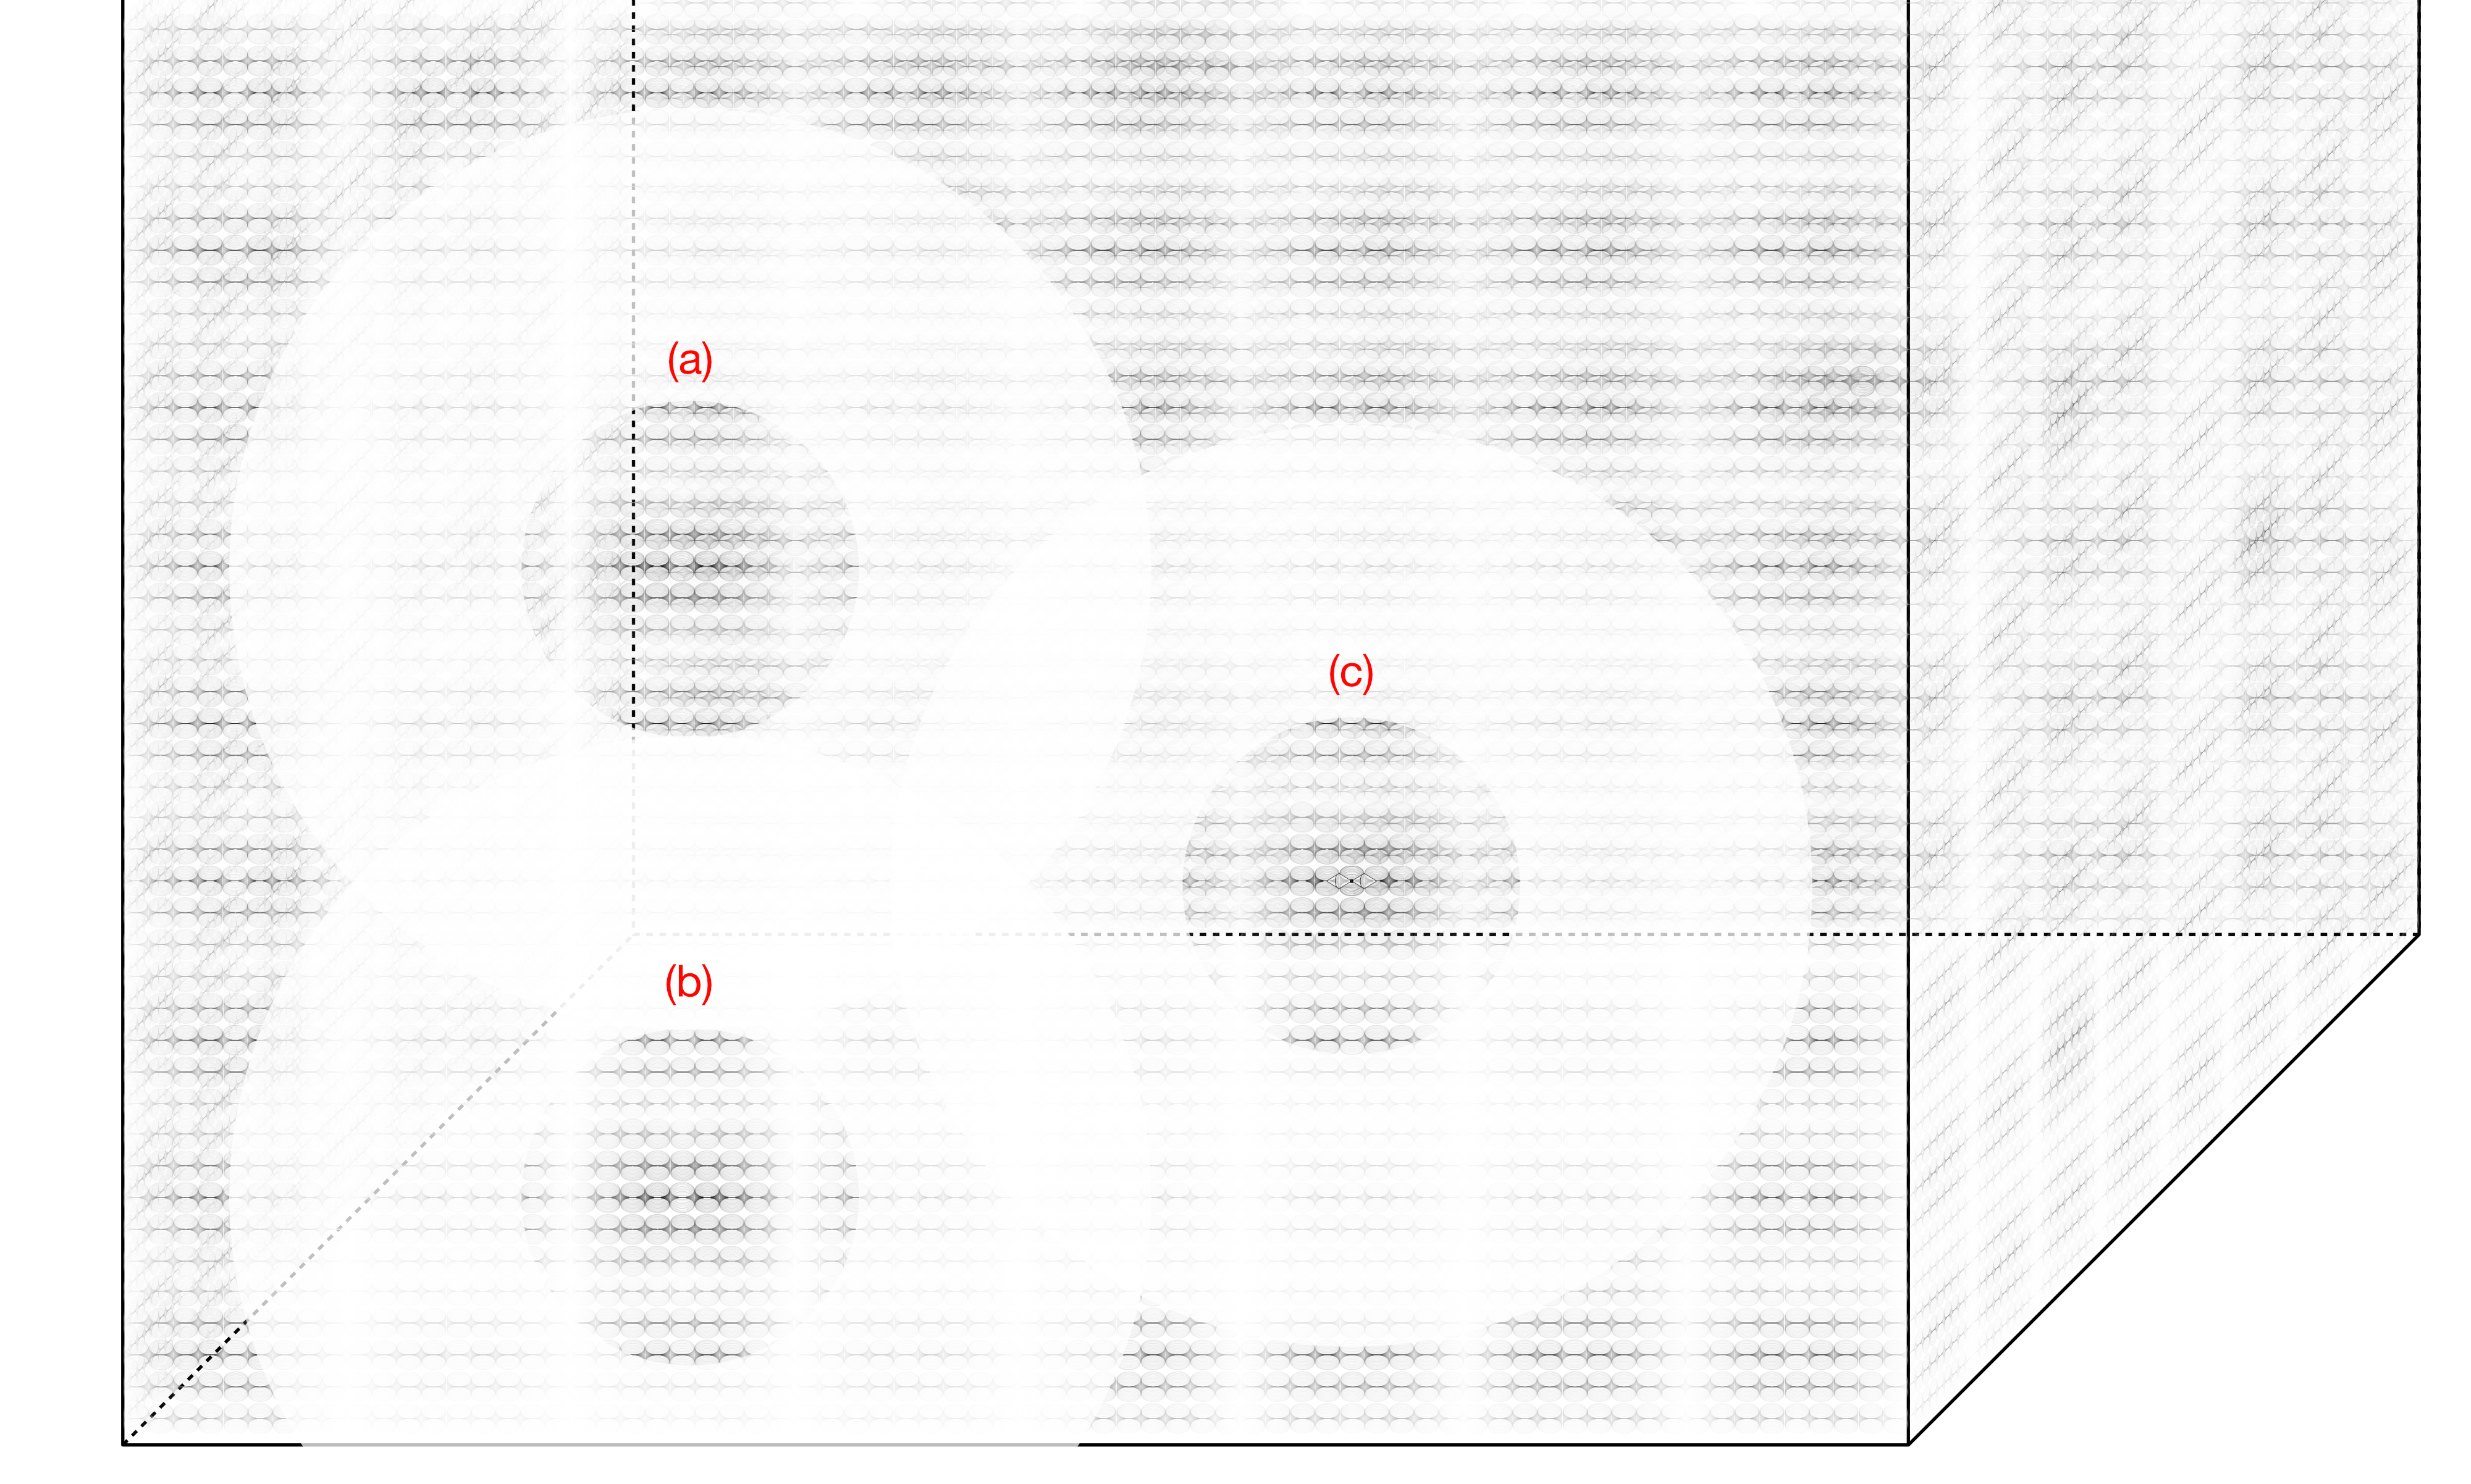
\includegraphics[width=0.7\linewidth]{figures/4.5.png}
    \caption[Larger field of horn tori as point plot heatmap]
    {\textbf{Larger field of horn tori as point plot heatmap.}}
    \label{f4.5}
\end{figure}
\FloatBarrier


\FloatBarrier
\section{Experiment to test computational information management of a hyperlinked research database}
\begin{figure}[h]
    \centering
    \includegraphics[width=\linewidth]{figures/4.6.png}
    \caption[Obsidian network graph of my research database and detail]{\textbf{Obsidian network graph of my research database and detail.}}
    \label{f4.6}
\end{figure}
\index[terms]{network graph}
\FloatBarrier

To test the production of network graphs in PKM, I began my work with Obsidian, a markdown language platform that allows users to hyperlink across text files \citep{obsidian_obsidian_nodate}. Obsidian user databases are called vaults, individual text files are called pages, bulleted lines of text are called blocks, and hyperlinks are called links. Users of Obsidian’s predecessor Roam Research \citep{roam_research_roam_nodate} or other similar platforms like Logseq \citep{logseq_logseq-_nodate} may be familiar with some of the terminology and Markdown language formatting \citep{gruber_markdown_2004, swartz_html2text_2011}. 
\index[people]{Swartz, Aaron}
\index[people]{Gruber, John}

I set up my workflow for collecting sources and linking them following courses by Danny Hatcher \citep{hatcher_become_nodate} and Lisa-Marie Cabrelli \citep{cabrelli_roam_nodate}. I consulted with Jay L. Colbert \citep{colbert_about_2022} to set up synchronization of my Obsidian and Logseq databases. 


As part of my survey of similar platforms, I tested Logseq, which drew me in with its default mode for outlining text using collapsible lists of nested bullet points. I coded a Logseq index page that automatically listed all my database blocks under letters of the English alphabet, Arabic numerals, and Adler's set of 102 syntopical terms \citep{adler_great_1952-2}. Logseq's collapsible bullets were an especially valuable user interface feature in a long index page like mine, shortening scrolling time by tucking away blocks under their category name unless I actively clicked on a letter, number, or term of interest. 


The following Markdown code shows how I listed blocks from my database which start with the letter `a':

\begin{verbatim}
#+BEGIN_QUERY
{
  :title "Pages that start with a"
  :query [
    :find (pull ?p [*])
    :where [
      [?p :block/name ?name]
      [(clojure.string/starts-with? ?name "a")]
    ]
  ]
}
#+END_QUERY
\end{verbatim}


I made my Logseq index page by modifying the string query code from Logseq discussion forum user starryvechsh \citep{noauthor_how_2022}. The full-length code for my Logseq index is available in \href{https://github.com/orusmateo}{my GitHub repository}. 

\index[people]{Adler, Mortimer J.}
\index[terms]{Syntopicon}

\section{Experiment to test topic modelling between semantic fields for interdisciplinary Knowledge Translation}

Drawing on my lived experience of being raised Roman Catholic while working towards climate crisis mitigation, I made topic models using the platform InfraNodus \citep{paranyushkin_infranodus_nodate-2}\footnote{InfraNodus uses the Louvain community detection algorithm proposed by Blondel et al. \citep{blondel_fast_2008,paranyushkin_force_2022}; InfraNodus notes in a tool-tip within the interface that its High-Level Ideas were generated using GPT-4. } of the papal encyclical \textit{Laudato si’} \citep{bergoglio_laudato_2015} and the \textit{Synthesis Report of the IPCC Sixth Assessment Report} \citep{lee_ipcc_2023} to graph intersecting themes in pursuit of Knowledge Translation across semantic fields, and to better understand both texts in relation to each other. The result included ten labels for groups of intersecting: (1) development equity, (2) environmental justice, (3) climate emissions, (4) disaster risk, (5) community development, (6) religious ethics, (7) global emissions, (8) climate resilience, (9) climate action, and (10) sustainable energy. 


\index[people]{Paranyushkin, Dmitry}
\index[terms]{InfraNodus}
\index[terms]{Knowledge Translation (KT)}
\index[terms]{climate resilience}
\index[people]{Francis, Pope}
\index[terms]{Intergovernmental Panel on Climate Change (IPCC)}
\index[terms]{Knowledge Translation (KT)}
\index[people]{Francis, Pope}



\begin{figure}[h]
    \centering
    \includegraphics[width=0.6\linewidth]{figures/4.8.png}
    \caption[Topic model of themes shared between two texts]{{\textbf{Topic model of themes shared between two texts.} Graph of themes present in both \textit{Laudato si'} \citep{bergoglio_laudato_2015} and the \textit{Synthesis Report of the IPCC Sixth Assessment Report}} \citep{lee_ipcc_2023}. Ten high-level ideas are identified here by InfraNodus and labelled in bright colours as (1) development equity, (2) environmental justice, (3) climate emissions, (4) disaster risk, (5) community development, (6) religious ethics, (7) global emissions, (8) climate resilience, (9) climate action, and (10) sustainable energy. Generated in InfraNodus and used with permission.}
    \label{fig:4.8}
\end{figure}
\index[terms]{Intergovernmental Panel on Climate Change (IPCC)}
\index[people]{Francis, Pope}
\index[terms]{climate resilience}
\FloatBarrier

\clearpage
\par
I found that there are concepts present in the \textit{Synthesis Report of the IPCC Sixth Assessment Report} but missing in \textit{Laudato si'}, and vice versa. I was concerned that ‘adaptation’ and ‘mitigation’ were not a part of \textit{Laudato si’}. Conversely, the \textit{Synthesis Report of the IPCC Sixth Assessment Report} did not include the terms `god’ and `church,’ which is unsurprising considering it is not a theological document.

InfraNodus also provided a list of entry points to develop each text, which it calls \textit{conceptual gateways}. In addition to the previous missing concepts to develop \textit{Laudato si’}, this topic model recommended developing the ideas of `infrastructure’ and `warming.’ 

While neither document fully represents climate science or theology, topic modelling across disciplines using InfraNodus was a promising example of emerging computational techniques for interdisciplinary climate text analysis.

\index[people]{Francis, Pope}
\index[terms]{Intergovernmental Panel on Climate Change (IPCC)}
\index[terms]{InfraNodus}


\begin{figure}[h]
    \centering
    \includegraphics[width=0.8\linewidth]{figures/4.9.png}
    \caption[Missing Concepts comparison]
    {\textbf{Missing Concepts comparison.} \textit{Left}: concepts in the Synthesis Report of the \textit{IPCC Sixth Assessment Report} but missing from \textit{Laudato si'}. \textit{Right}:  concepts in \textit{Laudato si'} but missing from the Synthesis Report of the \textit{IPCC Sixth Assessment Report}. Left and right Missing Concepts lists were generated under the Blind Spots tab in the Text Analytics Panels of InfraNodus, and shown side-by-side here for comparison. Used with permission.}
    \label{fig:4.9}
\end{figure}
\index[terms]{Intergovernmental Panel on Climate Change (IPCC)}
\index[terms]{InfraNodus}
\index[people]{Francis, Pope}

\begin{figure}[h]
    \centering
    \includegraphics[width=0.8\linewidth]{figures/4.10.png}
    \caption[Conceptual Gateways comparison]
    {\textbf{Conceptual Gateways comparison.} \textit{Left}: gateways for \textit{Laudato si'}. \textit{Right}: gateways for the \textit{Synthesis Report of the IPCC Sixth Assessment Report}. Left and right Conceptual Gateways lists were generated under the Blind Spots tab in the Text Analytics Panels of InfraNodus, and shown side-by-side here for comparison. Used with permission.}
    \label{fig:4.10}
\end{figure}
\index[terms]{Intergovernmental Panel on Climate Change (IPCC)}
\FloatBarrier
\index[terms]{InfraNodus}
\index[people]{Francis, Pope}

\clearpage


\section{Experiment to test more ecological local AI}
\begin{quote}
    ``\textit{The ecology of the vast symbolic world has to be supported by a material infrastructure of sustainability and responsibility, and turning our back on the real is no way to guarantee the virtual}” \citep[p. 196]{drucker_graphesis_2014}. 
\end{quote}
Since my thesis works to apply the ``studio laboratory of knowledge design” \citep[p. 197]{drucker_graphesis_2014}  and ``knowledge engineering” \citep[p. 8]{wielinga_kads_1992}  behind Sustainability Transitions Knowledge Activation, it is foundational to approach this work while managing its ecological cost. AI, in particular, has a large and growing cost that is ``widening disparity in how different regions and communities are affected” \citep{ren_uneven_2024}. 
\index[terms]{Sustainability Transitions} \index[terms]{Knowledge Activation (KA)} \index[terms]{Sustainability Transitions Knowledge Activation (STKA)} 
\index[people]{Drucker, Johanna}

Considering the environmental costs of using AI, I moved to test topic modelling using Small Language Models that can run on my local workstation. Computer scientist Rahul Nayak proposes one such solution to create what he refers to as graphs of concepts using Mistral 7B, named after its comparably small seven billion parameters \citep{nayak_how_2023}.
\index[terms]{Large Language Model (LLM)} 
\index[terms]{Small Language Model (SLM)} 
\index[terms]{Language Model (LM)} 

Software engineer Juan Sulca and I successfully used Nayak’s method to create a navigable and searchable graph of concepts of \textit{Laudato si’}. However, further development would be required to create a comparison graph such as the one generated by InfraNodus.
\index[terms]{InfraNodus}
\index[people]{Francis, Pope}

\FloatBarrier
\begin{figure}[h]
    \centering
    \begin{minipage}[t]{0.48\linewidth}
        \centering
        \includegraphics[width=\linewidth]{figures/4.11.png}
        \caption[Overview of the \textit{Laudato si'} graph of concepts]    {\textbf{Overview of the \textit{Laudato si'} graph of concepts.} Topic model made using Rahul Nayak’s Mistral 7B method \citep{nayak_how_2023}.}
        \label{f4.11}
    \end{minipage}%
    \hfill
    \begin{minipage}[t]{0.48\linewidth}
        \centering
        \includegraphics[width=\linewidth]{figures/4.12.png}
          \caption[Detailed view of the \textit{Laudato si'} graph of concepts]    {\textbf{Detailed view of the \textit{Laudato si'} graph of concepts.} Topic model made using Rahul Nayak’s Mistral 7B method \citep{nayak_how_2023}.}
        \label{f4.12}
    \end{minipage}
\end{figure}
\index[people]{Francis, Pope}

\par

\FloatBarrier

\section{Stewarding knowledge for climate resilience}
A number of political and economic factors actively detract from climate mitigation. For example, hyper-specialization is convenient for the current predominantly empire-driven capitalist extractivist economy; hyper-specialization makes humans monocrops for convenient harvesting through overwork, which keeps large populations subjugated as politically docile consumers. It seems to me that it is convenient to keep researchers underinformed about solutions from other fields that support climate crisis mitigation. This means solutions can be bought and sold to maintain control of populations. Specialization is required to achieve proficiency and make an impact in any field, but isolation-reinforced hyper-specialization does not have to be the norm.
\index[terms]{network graph}

As the earth careens toward catastrophe, resistance will inevitably ensue, and oppressors will have the prerogative to control populations by harsher means. The university context has historically facilitated resistance against the ideological and technological structures that limit climate justice and climate resilience. Discussing my research has taught me that many organizations, including universities, struggle to best use available information to facilitate researcher grouping, which significantly restricts funding for many deserving initiatives. In my pursuit of building better tools for connecting ideas, I also aim to connect the people who have them. Doing both makes it more likely that we will reveal solutions for climate crisis mitigation that may exist in the information we already have. 
\index[terms]{climate justice}
\index[terms]{climate resilience}
\chapter{From theory and method to visuospatial models and back}

\section{From theory to visuospatial models}

\noindent The following contributions are ways visuospatial models encapsulate theories from my literature review as contributions 1, 2, and 7: Semantic Forms, Query Isomorphs, and TCA Workspace, respectively. \index[terms]{Semantic Forms} 
\index[terms]{Query Isomorphs} \index[terms]{TCA Workspace}

\subsection{Contribution 1. Semantic Forms}
\begin{itemize}
        \item[\textbf{C1}] \textit{Semantic Forms}, a taxonomy of three-dimensional topic model compositions for HITL CATG, HATG, or both.
\end{itemize}

\subsubsection{Vedic entry point to visuospatial epistemology}
A key outcome of my survey of symbols was arriving at two- and three-dimensional representations. Studying the Sri Yantra and the Meru Chakra together catalyzed a significant shift in my work, expanding it from visual to visuospatial epistemology of information visualization and network graphs. This occurred in two steps. 
\index[terms]{Sri Yantra} \index[terms]{Meru Chakra}  \index[terms]{network graph} \index[terms]{visuospatial epistemology}

First, I read the Sri Yantra as a network graph, which extended its significance in my work beyond its more conventional appreciation as a representation of spiritual qualities to the more etymologically encompassing range of the word \textit{yantra} which includes the practical and mechanical attributes of an 'instrument' or 'machine' \citep[p. 28]{buhnemann_mandalas_2003}. The numerous overlapping triangles of the Sri Yantra evoked a sense of movement for me, like moving network graphs of nodes and edges.

Second, I encountered the Meru Chakra in relationship to the Sri Yantra as interdimensional 2D-3D representations of each other. I propose that signify meaning in both their individual complexity and in the way they hold space for meaning across dimensions. This tension across dimensions catalyzed my ongoing fascination with visuospatial epistemology and the various ways we convey meaning using visuospatial signs \citep{anderson_drawing_2018,drucker_graphesis_2014,dubois_systematic_2002,midgley_theory_1998,sevaldson_designing_2022,tversky_barbara_2022}.
\index[terms]{visuospatial epistemology} \index[people]{Drucker, Johanna} \index[people]{Tversky, Barbara} \index[people]{Sevaldson, Birger} \index[people]{Anderson-Tempini, Gemma}
\index[people]{Dubois, Anna} \index[people]{Gadde, Lars-Erik} \index[people]{Midgley, Gerald} 
\index[terms]{visuospatial epistemology}

\subsubsection{Defining Semantic Forms}
My proposal of Semantic Forms in this thesis does not include comprehensive technical specifications for how to algorithmically build them. Instead, I focus on what researchers might do with Semantic Forms if and when they are developed. I make the assumption that it is possible for Semantic Forms to work with vector embeddings and network graphs. I also conjecture that rich TCA graphs can be used to train Language Models by parsing visuospatial forms of knowledge activation.
\index[terms]{Large Language Model (LLM)} 
\index[terms]{Small Language Model (SLM)} 
\index[terms]{Language Model (LM)} 

The sense of visuospatial affords humans a higher bandwidth for information processing than just two-dimensional representation \citep{tversky_barbara_2022}, which could hold a key for managing the complexity of the climate crisis, or at the very least engaging with it with more agency. This section, however, is about the visuospatial models I made and not about their application to climate. 

As an interface, Semantic Forms are dimensionally versatile three-dimensional visuospatial point cloud compositions that can be dimensionally reduced to produce two-dimensional information representations. As a computational tool using Topological Capta Analysis on high-dimensional graphs, dimensional reductions would occur across a much wider range of dimensions. 

In the following section, I describe the geometric fundamentals I derived from surveying two-dimensional information visualization composition; then, as a means of Meta-Systematic Combining (MSC), I added a third dimension. I called the two-dimensional compositions I derive \textit{Semantic Shapes}, and the three-dimensional compositions I derive \textit{Semantic Forms}. I will write geometric shapes and forms in lowercase, like ``circle" and ``sphere"; I will write the shape identifiers names of my Semantic Shapes and Semantic Forms in uppercase, like ``Circle Semantic Shape" and ``Sphere Semantic Form."
\index[terms]{Semantic Forms} \index[terms]{Semantic Shapes}  \index[terms]{Systematic Combining (SC)}


\subsubsection{Topology in Semantic Forms}
Filtration can be used to assess hierarchical structure in weighted networks \citep[p. 11]{giusti_twos_2016}. Therefore, filtration can facilitate Query Isomorph queries across Semantic Forms with a rigorous inspection process of all nodes and edges in a network, allowing the identification and analysis of network isomorphologies across a variety of network formations, nested and hierarchical or not.
\index[terms]{isomorphology} \index[terms]{topology} 

While filtration is necessary for managing higher-dimensional graphs or graphs with a high density of nodes, I offer a complimentary analogy of magnetic form types. These magnetic form types would affect the distribution of nodes and edges in space in distinct arrangements. The Cone Semantic Form, for example, could distribute topic model graph nodes to reveal the divergence or convergence of ideas in a given text. 
\index[terms]{analogy} 
\index[terms]{Cone Semantic Form} 
\index[terms]{morphology}
\index[terms]{isomorphology}

The value of investigating Semantic Shapes and Semantic Forms was supported for me in more contemporary topological literature about network weighting. The torus and the disc are closely related to the forms uniquely suited to manage Global Topological Synchronization (GTS). \footnote{According to Wang et al., two weighted simplicial complexes, the Weighted Triangulated Torus and the Weighted Waffle ``can sustain global synchronization of edge signals” \citep[p. 9]{wang_global_2024}.} We are one step closer to higher-dimensional topic models in which the physical representations of node relationships represent and reveal more complex semantic relationships like syntopical consiliences.
\index[terms]{syntopical consilience} \index[terms]{Semantic Forms} \index[terms]{Semantic Shapes}  \index[terms]{simplicial complex} 
\index[terms]{consilience}

\subsubsection{Magnetic approach to node groups using weighted graphs}
While existing approaches emphasize filtration \citep[p. 11]{giusti_twos_2016}, edge weighting for managing a large number of nodes \citep{kovacs_iterative_2024}, and self-organizing bundling for emphasizing node relationships to increase their visibility \citep[p. 1]{holten_forcedirected_2009}, the literature considered for this thesis did not find any approaches that considered a taxonomical account of the semantic value of geometric forms for their use in the diachronic, topological, and systematic analysis of network graphs of texts.

Building onto the current practices of network graph filtering and labelling nodes using the semantic value of shapes or forms, I propose Semantic Forms as a new approach for revealing semantic relationships in text graphs. One way this would be achieved is by quantifying Peircean modes of reasoning as a means of node clustering. The Semantic Forms, then, would act as ‘magnetic’ fields which influence the placement of nodes and edges in a topic model graph. Depending on the researcher's aims, these semantic forces would act as an organizing principle that influences all graph nodes or a filtered few. Semantic Forms are, in a sense, semantic forces captured as geometric patterns; they are not prescriptive but are meant to be used to arrange nodes in space to reveal characteristics and patterns within a set of topics. By building on the affordances of three- rather than two-dimensional space, emphasizing node arrangement rather than filtering out potentially valuable contextual nodes, Sematic Forms would improve the identification of more relevant nodes and node relationships.
\index[people]{Peirce, Charles Sanders} 

Weighting a network with the characteristics of Peircean induction, deduction, and abduction would imbue network relationships with useful information for clustering nodes in the virtual semantic field using Semantic Forms. For example, Ontological Semantic Network Summaries (OSNS) can be used to determine the semantic (1) impact and (2) ‘direction’ catalyzed by a given term. For example, in the literature of Aristotle, the practice of categorization would (1) be quantified as having a very high impact; (2) its direction would be (2.1) inductive, as a practice for moving from specific observations to general, or syntopically consilient, conclusions, (2.2) deductive, as a prescription for ontological analysis (e.g. the Tree of Porphyry as semantic network of ontology \citep[p. 4-5]{sowa_knowledge_2000}), (2.3) abductive, defined in a Peircean way, as a means of innovating an explanation in compliment to inductive and deductive reasoning \citep[p. 106]{peirce_pragmatism_1960}. For example, in the study of cognition, categorization is both (a) a phenomenon that can be observed as being comprised of specific characteristics and (b) a means of studying a given subject.
\index[people]{Peirce, Charles Sanders} 
\index[people]{Aristotle}
\index[people]{Porphyry}
\index[terms]{Ontological Semantic Network Summaries (OSNS)} \index[terms]{Global Topological Synchronization (GTS)} \index[terms]{abduction}
\index[terms]{Tree of Porphyry}


\subsubsection{Semantic Shapes: two-dimensional geometric network graph}
Parting from the assumption that dots and lines are the necessary representation of one-dimensional linear relationships, or \textit{Semantic Lines}, I developed a list of two-dimensional shapes which summarize node-radiality compositions used in the organization of network graph information visualizations\footnote{Rendgen et al.’s \textit{History of Information Graphics} \citep{rendgen_history_2019} provide a rich source matter for analyzing information visualization composition. Anna Vital’s infographic of infographics \textit{How to think visually using visual analogies} \citep{vital_how_2018} and \textit{The Data Visualisation Catalogue} by Severino Ribecca \citep{ribecca_data_2017} provide categorizations of information visualization compositions types. I found that individual units of information, dots or otherwise, were laid out away from each other in varying radiality configurations with distinct semantic affordances.}, or what I am naming \textit{Semantic Shape}. The rectangle Semantic Shape can be used to illustrate grids, the triangle Semantic Shape can be used to illustrate hierarchical relationships or contingencies, and the Circle Semantic Shape can represent a multidirectional array of triangular Semantic Shapes.
\index[people]{Vital, Anna} \index[people]{Ribecca, Severino} \index[terms]{Semantic Shapes} \index[terms]{Semantic Line} 

\FloatBarrier
The limited number of individual relationships a node can have in a rectangle Semantic Shape benefits applications like algorithmic quantitative analysis in spreadsheets. However, qualitative analysis benefits from the larger range and variable number of nested node relationships possible in the triangle and Circle Semantic Shape. My focus in the following work favours the triangle and Circle Semantic Shape and their role in categorizing compositions for node graph information visualization.
\index[terms]{Semantic Shapes} 

\begin{figure}[h]
    \centering
    \includegraphics[width=0.8\textwidth]{figures/5.1.png}
    \caption[Network graphs as Semantic Shapes]
    {\textbf{Network graphs as Semantic Shapes}. \textit{Left}: Semantic Line one-dimensional network graph line. \textit{Right}: Semantic Shape two-dimensional network graph radiality compositions: the Rectangle, Triangle, and Circle.}
    \label{f5.1}
\end{figure}


\begin{figure}[h]
    \centering
    \includegraphics[width=0.8\textwidth]{figures/5.2.png}
    \caption[Example of circle and triangle Semantic Shape nested in a larger Circle Semantic Shape network graph]
    {\textbf{Example of Circle and Triangle Semantic Shape nested in a larger Circle Semantic Shape network graph.} \textit{Top left}: Obsidian graph view of my research database. \textit{Top right}: Zoomed view of region marked with yellow-green box. \textit{Bottom}: Labelled Semantic Shape on clusters of network nodes.}
    \label{f5.2}
\end{figure}

\FloatBarrier
%Manuel Lima’s categorization of information visualizations circles and trees \citep{lima_book_2014,lima_book_2017} corroborate the value of my proposal for a Circle Semantic Shape and the triangle Semantic Shape as trees. 

\subsubsection{Semantic Forms: three-dimensional composition types in network graphs}
Moving from one-dimensional network graph lines to two-dimensional network graphs, Semantic Shape laid the groundwork for adding a third dimension to my network graph models and a resulting list of \textit{Semantic Forms}. I approached this exercise as both a deconstruction of complex forms and a combination of Semantic Shape. 
\index[terms]{Semantic Shapes} \index[terms]{Semantic Forms} 


\paragraph{Deconstruction of complex forms} \mbox{} \\

Calling back to my preceding work involving visualizations of Vedic principles, namely the chakras, perhaps the most pivotal bridge for me from theological research to this investigation of network graphs was through Vedic spiritual imagery. In particular, two interrelated forms were the object of my delight and fascination: the Sri Yantra and the Meru Chakra. I studied Vedic spirituality under the guidance of Dr. Monisha Bhatia. However, my work in this thesis will emphasize the geometric and visuospatial attributes of the Sri Yantra and the Meru Chakra, rather than understandings of their cosmological attributes.
\index[terms]{Sri Yantra} \index[terms]{Meru Chakra} 
\index[people]{Bhatia, Monisha}

Encountering that a two-dimensional graph of lines like the Sri Yantra could interrelate with a three-dimensional visualization like the Meru Chakra encouraged me to consider the opportunities available in dimensional addition to flat graphs. 
\index[terms]{Sri Yantra} \index[terms]{Meru Chakra} 

By averaging out the different steps, or elevations, of the Meru Chakra, which has “the form of a mountain” \citep[p. 31]{buhnemann_mandalas_2003}, the cone form is evident in its composition. The Sri Yantra itself is composed around a central point and its sets of triangles are outlined by a circle. I arrived at the geometric curiosity of a graph of lines that could be represented as both a circle and a cone, the former being more typical of an information visualization composition and the latter being novel for me as a method for the semantic representation of individual elements in a graph. 
\index[terms]{Sri Yantra} \index[terms]{Meru Chakra} 

Upon considering the shape of the horn torus, its two horn-shaped negative-space dimples are shaped like cones. Motivated by this geometric curiosity, I considered how other simple forms could be understood as parts of the horn torus. Following this line of reasoning, I arrived at the cylinder as the horn torus’s body, which is also the body of a ring torus. Here, I call back to my preamble work, where I illustrated how a series of horn tori form double cones. At this point, it was easy to envision a horn torus without its double-dimple as a network of nodes organized around a central point or a sphere. Through this deconstruction process, in order of arrival, I list here six Semantic Forms: the Horn Torus, the Cone, the Ring Torus, the Cylinder, the Double-Cone, and the Sphere. 
\index[terms]{horn torus} 
\index[terms]{ring torus}
\index[terms]{cylinder}
\index[terms]{cone}
\index[terms]{sphere}
\index[terms]{Horn Torus Semantic Form}
\index[terms]{Ring Torus Semantic Form}
\index[terms]{Cylinder Semantic Form}
\index[terms]{Cone Semantic Form}
\index[terms]{Sphere Semantic Form}


\paragraph{Combination of Semantic Shapes} \mbox{} \\

Through the combination of Semantic Shapes, conversely, to the previously explained process of deconstruction, I arrived at the same six Semantic Forms. I illustrate how in \autoref{f5.3}. I begin with the PKM graphs from Obsidian and Logseq, which are disc-like Circle Semantic Shapes of nodes. I considered a simple dimensional addition to the Circle, which was to add linear extrusion along a perpendicular axis, creating a Cylinder. I added another form of circular complexity to the Cylinder by circling it in on itself into a Ring Torus. Next, I combined the Triangle and the Circle Semantic Shapes to arrive at the Cone and the Double Cone. Next,  I consider the perpendicular placement of two Circle Semantic Shapes intersecting at their centres by which I arrive at the Sphere. Last, I consider that the Ring Torus can be narrowed to shrink its inner radius to a single point, which makes a Horn Torus.
\clearpage
 \index[terms]{Semantic Shapes} \index[terms]{Semantic Forms} 
 
\FloatBarrier
% First Figure
\begin{figure}[p] % Use [p] to place it on a separate page if needed
    \centering
    \includegraphics[width=0.8\textwidth]{figures/5.3.png}
    \caption[Semantic Forms derived from the Circle Semantic Shape and other Semantic Forms]
    {\textbf{Semantic Forms derived from the Circle Semantic Shape and other Semantic Forms.} Systematic Combining was used as dimensional addition to move from two-dimensional to three-dimensional network graph compositions.}
    \label{f5.3}
\end{figure}

% Second Figure
\begin{figure}[p] % Use [p] to place it on a separate page if needed
    \centering
    \includegraphics[width=0.8\textwidth]{figures/5.4.png}
       \caption[Knowledge graph disc and six Semantic Forms]
        {\textbf{Knowledge graph disc and six Semantic Forms}: (a) Circle Semantic Shape knowledge graph, b) Cylinder Semantic Form, (c) Ring Torus Semantic Form, (d) Cone Semantic Form, (e) Double-Cone Semantic Form, (f) Sphere Semantic Form, and (g) Horn Torus Semantic Form. The top row includes more basic forms, and the bottom row includes more geometrically complex ones.}
    \label{f5.4}
\end{figure}
\FloatBarrier

\index[terms]{Ring Torus Semantic Form}
\index[terms]{Horn Torus Semantic Form}
\index[terms]{Cone Semantic Form}
\index[terms]{Double-Cone Semantic Form}
\index[terms]{Sphere Semantic Form}
\index[terms]{Cylinder Semantic Form}



\par
The Semantic Forms are means of three-dimensional topic model node clustering in a semantic field of terms, which reveal relationships like (1) ontological hierarchy of Peircean reasoning modes in which a singular term expresses a general principle and diverse instances of that general principle, (2) cyclicality, and (3) other modes of semantic relationship interpretation in the visuospatial. As a means of capturing hierarchical semantic systems, Semantic Forms have the capacity to nest other Semantic Forms within themselves.
\index[terms]{Semantic Forms}
\index[people]{Peirce, Charles Sanders}

\textbf{The Cone Semantic Form} is perhaps the most direct illustration of this principle because its form physically turns to a single point. \textbf{The Sphere Semantic Form} encompasses a higher number of radii, which accommodates multiple Cones converging to a single point or a series of nested convergence points. \autoref{f6.1},\textit{The Ontological Semantic Network Summary of the Syntopicon’s Great Ideas onto the Tree of Porphyry}, is an example of a dimensionally reduced Cone Semantic Form of consilience-oriented information categorization. \autoref{f6.1} demonstrates that Sowa's sense of philosophical-computational ontology and Adler's interdisciplinary term-indexing \citep{adler_great_1952-2} can be understood as a single system through Aristotelian categorization and Porphyrian semantic network graphing \citep[p. 4-5]{sowa_knowledge_2000}. \textbf{The Cylinder Semantic Form} provides an extruded space of the flat circular graph and traces individual nodes or graphlets across a third axis representing time as a quantified Semantic Line. \textbf{The Ring Torus Semantic Form} accommodates the cone as a structure that feeds back to itself in a cycle. 

The \textbf{Horn Torus Semantic Form} accommodates multiple cycles that exhibit transformation and feeding back into themselves by emerging from a point, changing, and then returning to that same re-origin point. The horn torus has the distinct ability to nest two cone-like structures in its negative space as an opportunity to capture or reveal additional semantic relationships. For instance, a moving Horn Torus Semantic Form network graph, which is used to topic model a text and identify a re-origin point, can also capture the deductive and inductive changes in relationships between ideas in that text or between this given text and other texts by using the horn torus negative-space horn dimples as Cone Semantic Forms. The Cone Semantic Form can be used on its own to model the deductive and inductive reasoning in a text or texts, of course. Static Horn Torus Semantic Form models can benefit from moving components to represent change over time for shifts of reasoning, iterations, building texts onto one another, or changes of popular opinion. Moving horn toroidal models could also be overlaid with each other to compare arguments and isomorphologies of reason.

\index[terms]{Ring Torus Semantic Form} 
\index[terms]{Query Isomorphs}
\index[terms]{Horn Torus Semantic Form} 
\index[terms]{horn torus}
\index[terms]{Cylinder Semantic Form} 
\index[terms]{Semantic Line} 
\index[terms]{Syntopicon} 
\index[terms]{Tree of Porphyry} 
\index[terms]{Ontological Semantic Network Summaries (OSNS)}
\index[people]{Porphyry}
\index[people]{Sowa, John F.}
\index[terms]{consilience}


\paragraph{Moving Semantic Forms} \mbox{} \\
To render the three-dimensional network graphs of these six Semantic Forms, I used Blender to create moving network graph point clouds using Manuel Casasola Merkle’s plexus effect node programming tutorial \citep{casasola_merkle_blender_2022}.
\index[terms]{Blender (software)}

The resulting models captured my idea for a topic modelling interface that uses three-dimensional network graph Semantic Forms with more clarity. The information visualization encoding of Semantic Forms as interface would label categorical and sequential differences between groups of related ideas using nodes colours. Ideas that can be listed across categories would be identified using edges with colours that gradiate between origin the two different node colours. Moving nodes would represent changes in a database over time including occasions when ideas displace or replace other ideas.
\index[terms]{Semantic Forms} \index[terms]{network graph} 

As moving network graph representations of computational text analysis, my Semantic Forms exemplify how Anderson-Tempini's isomorphogenesis \footnote{Isomorphogenesis is described in more detail \autoref{Interdisciplinary visual methods}. As a brief reminder, Anderson-Tempini's term isomorphogenesis refers to the extension of her isomorphology practice used for exploring ``the potentialities of representing morphology as a dynamic and formative process” \citep[p. 179]{anderson_drawing_2018}.} is echoed in Drucker: “We will use the interpretative force of graphical rhetoric as a gesture language of intellectual life, as a way of shaping our communication using the variable dimensions of time and space in ways that print could only hint at, recording as it did the layered, palimpsestic traces of individual and collaborative activities on the enduring substrate of its material surfaces” \citep[p. 197]{drucker_graphesis_2014}. My moving Semantic Form models capture the way in which new information changes the shape of a visuospatial topic model. For a link to view my moving Semantic Forms, see \autoref{Appendix: Thesis website} of the Appendix.
\index[terms]{isomorphogenesis} \index[terms]{Semantic Forms} 
\index[people]{Drucker, Johanna} \index[people]{Anderson-Tempini, Gemma} 




\paragraph{Geometric analysis} \mbox{} \\
I found Semantic Forms are closely related to surfaces of revolution, meaning surfaces ``generated by rotating a two-dimensional curve about an axis” \citep{weisstein_surface_nodate}. Note the similarities to the Semantic Forms in the following examples: ``Examples of surfaces of revolution include the apple surface [similar to the horn torus], cone (excluding the base),[...] cylinder (excluding the ends),[...] lemon surface [similar to the double cone], [...] sphere, [...] and torus” \citep{weisstein_surface_nodate}. At the outset of my research I considered how new forms of spatial network graphs would plot \textit{into} the Semantic Forms, so I considered their surfaces after.
\index[terms]{torus} 
\index[terms]{surfaces of revolution} 
\index[terms]{Semantic Forms} 
\index[terms]{Personal Knowledge Management (PKM)} 
\index[terms]{Ring Torus Semantic Form}
\index[terms]{Sphere Semantic Form}


I anticipate working with Semantic Forms in relation to surfaces of rotation will lead to new methods of network graph plotting. To begin the differentiation of the Semantic Forms’ volume and surface for the next steps of their geometric analysis, I list the Semantic Forms’ volume and surface equations in Cartesian coordinates as a in Appendix \autoref{Semantic Forms equations}.

\index[terms]{torus} 
\index[terms]{surfaces of revolution} 
\index[terms]{Semantic Forms} 
\index[terms]{Personal Knowledge Management (PKM)} 
\index[terms]{Ring Torus Semantic Form}
\index[terms]{Sphere Semantic Form}


\paragraph{Tidiness of the Semantic Form models} \mbox{} \\
While I am observing the geometry of such compositions and providing examples that neatly showcase their shapes and forms, I am not claiming to advocate for node-by-node retrofitting to fit these models, which would be a disservice to the data. Finding patterns in data is difficult in two dimensions, let alone any dimensions above it. In future work, I will investigate mathematical approaches for identifying Semantic Form patterns in large network models of computationally modelled data. The focus of this work is to identify the semantic value of an array of shapes and forms so as to establish which patterns to look for. The finding of these patterns in real data is for another work. \\

By making Semantic Forms, I sought to define the ways geometric form can be given topological versatility in the ways large groups of nodes reveal group semantic relationships, similar to Global Topological Synchronization \citep{bianconi_topology_2024,wang_global_2024}. In the following section, I aim to focus on the smaller network chunks within these more macroscopic murmurations. 
\index[terms]{Semantic Forms} 
\index[terms]{Global Topological Synchronization (GTS)} 
\index[terms]{topology}
\index[people]{Bianconi, Ginestra}
\index[terms]{Semantic Forms}
\clearpage




\section{Contribution 2: Query Isomorphs}
\begin{enumerate}
        \item[\textbf{C2}] \textit{Query Isomorphs} as a means of Topological Capta Analysis (TCA) in HITL CATG using small graph chunks.
\end{enumerate}


\subsection{Defining the Query Isomorph}

I define Query Isomorphs as isomorphic directed graphlets as dimensionally versatile query objects and query interfaces. In this section I explain the meaning embedded in the terms `isomorph' and `query'.


\paragraph{`Isomorph'} \mbox{} \\
The earliest record of the word isomorph I found was by 19th century chemist Eilhard Mitscherlich, as I mention in my introduction, who uses isomorph to describe `sameness of form.' More specifically, Mitscherlich is known for discovering the the law of isomorphism which links a substance's crystal structure to its chemical composition \citetext{\citealp[p. 239]{Berzelius1821Loethrohr}; \citealp{the_editors_of_encyclopaedia_britannica_eilhardt_2024}; \citealp [p. 427-437]{Mitscherlich1820Abhandlungen}; \citealp[p. 239]{Mitscherlich1837Lehrbuch1}}.
\index[terms]{isomorphism}
\index[people]{Mitscherlich, Eilhard}

Borrowing the isomorphism principle from chemistry, I anticipate a link between a text corpus's spatial network graph `crystalizations' and its `datacule' graphlet compositions. I also anticipate that the application of computational chemistry methods like AlphaFold \citep{alphafold_alphafold_2023} will accelerate information science approaches for finding latent isomorphic semantic relationships (problems/solutions, risks/opportunities, etc.) across academic disciplines. The impact of such systems would not only benefit Sustainability Transitions, but all areas of research.
\index[terms]{isomorphism}

Applying computational chemistry to work with isomorphic semantic relationships also has an opportunity to capture semantic change in graphs of three and many more dimensions. Therefore, I also anticipate that the versatility of topology will help working with isomorphic network graphlets across changing position, configuration, and dimension in high-dimensional hypergraphs. 
\index[terms]{isomorphism}

Isomorphism has had a wider range of applications than chemistry evidenced by the interdisciplinary work of Anderson-Tempini \citep{anderson_drawing_2018} across arts and sciences. Further to interpretive scope of this thesis, I align the Query Isomorph thought experiment substantially to Drucker's humanistic design. Drucker asserts that ``\textit{data are capta}, taken not given, constructed as an interpretation of the phenomenal world, not inherent in it" \citep[p. 128]{drucker_graphesis_2014}. The isomorphism of the Query Isomorph reveals what Drucker refers to as the ``constructedness of data as capta" \citep[p. 128]{drucker_graphesis_2014}. For these reasons, I also carry the interpretive interdisciplinarity of Anderson-Tempini's isomorphology in the term Query Isomorph in addition to its chemical origins. 

\index[terms]{morphology}
\index[terms]{isomorphology}
\index[terms]{isomorphism}
\index[terms]{Query Isomorphs}
\index[terms]{capta}


\paragraph{`Query'} \mbox{} \\
Computer scientist John. F. Sowa produced foundational work in the space of using graphs for querying information databases including the development of Query Graphs \citep[p. 313]{sowa_conceptual_1984}. I arrived at the idea of isomorphological query graphlets independently from Sowa, but our work overlaps and merits disambiguation. Query Graphs are related to my Query Isomorphs as mechanisms that help recognize patterns of meaning across different texts. However, Query Isomorphs differ from Query Graphs as \textit{dimensionally versatile} graph elements, which are queryable with TDA and TCA across the modes of KSSTP, and which also function as interface when in the visible three dimensions. The term Query Isomorph carries the term `Query' with respect of the shared lineage of computational graph-based text analysis that includes and has benefited from John F. Sowa's Query Graph development and pedagogy.


\index[terms]{Query Isomorphs} 
\index[terms]{Topological Data Analysis (TDA)}
\index[terms]{Topological Capta Analysis (TCA)}
\index[people]{Sowa, John F.}
\index[terms]{morphology}
\index[terms]{isomorphology}



\subsection{Making a Query Isomorph}

In this section I demonstrate how I designed a Query Isomorph using the literature review of this thesis by setting my semantic scope, and introducing my visualization design.

\subsubsection{Semantic Field \textit{S} and Sample \textit{s}}

To provide an example of the way Query Isomorph term nodes relate to Semantic Forms I set some parameters. Specifically, I set a semantic field, which is ``a set of words which cover a particular semantic domain and bear structured relations with each other" \citep[p. 107]{jurafsky_speech_2024}. 

To arrive at this list, I uploaded my thesis as a PDF to ChatGPT $4$o and parsed its keywords with the following prompt sequence: 

\begin{enumerate}
    \item[\textbf{1}] ``Categorize and list the key words in this document."
    \item[\textbf{2}] ``Write these as a list separated by commas, ranked by their relevance in the text"
\end{enumerate}
    
I imported this list of 756 Comma Separated Values (CSV) to Microsoft Excel.  Next, I reduced the number of terms on this list by removing redundant and less relevant words. I arrived at a list of 310 terms which I called Semantic Field \textit{S}. This list is included in Appendix \autoref{Appendix Semantic Field S}.
\index[terms]{Query Isomorphs}

Sample \textit{s} is a list of nineteen ideas which I arbitrarily selected from Semantic Field \textit{S} for having high importance in my thesis. In \autoref{tab:semantic_fields}, I list the terms from Sample \textit{s} along with the date of their earliest recorded use in my research database and a note of where the idea was first recorded. I use the word `idea' here and not `term' because some terms have changed over time. For example, I first named Query Isomorph `datacule’ as mentioned previously. The idea of isomorphic representations of ideas endures across the change from the term `datacule' to the term `Query Isomorph.' In a sense, this is an example of the textual isomorphogenesis of ideas about the visuospatial isomorphogenesis of ideas.
\index[terms]{Query Isomorphs}



I derived one term in particular as the most summatively descriptive through-line of this thesis: \textit{Computational Semiosis}. I arrived at this term in two steps. First, I drafted the graphs of Query Isomorph \textit{i} that you will encounter in this section, and arrived at the term \textit{Computational Graphesis}. This term encompassed the practice of applying computational methods like TCA to a wide array of ``visual forms of knowledge production" \citep{drucker_graphesis_2014}, what Drucker calls \textit{graphesis}. Seeking to build on Drucker's term by including Tversky's neuroscience of the visuospatial \citep{tversky_barbara_2022}, I returned to Drucker's Greek etymology of \textit{graphesis}. I derived \textit{semiosis} as more fitting for the sensorially decentralizing and diversifying scope of my \textit{visuospatial} forms of Knowledge Production. More specifically, I defined my use of the term semiosis in this thesis as Knowledge Activation across its various modes (KSSTP), and across the interrelated senses used in understanding, including but not limited to the visuospatial. For my updated through-line term, I arrived at the term \textit{Computational Semiosis}, which I included in \autoref{tab:semantic_fields} and the graphs that follow it.

\index[terms]{Query Isomorphs}
\index[terms]{Knowledge Production (KP)}
\index[terms]{Computational Semiosis}





\FloatBarrier
\begin{table}[htbp]
  \centering
  \begin{tabular}{p{0.4cm}p{4cm}p{2.5cm}p{5cm}}
      \toprule
      \textbf{\#} & \textbf{Sample \textit{s} term} & \textbf{Earliest use on record} & \textbf{Note (Place first used in my records and comment)} \\
      \midrule
      1 & Symbol-making & 2022 Jan and earlier & Prior studies: note-taking methods experimentation \\
      2 & Sri Yantra & 2022 Jan and earlier & Prior studies: theology \\
      3 & Network Graphs & 2022 Jan and earlier & Prior studies: note-taking methods \\
      4 & Meru Chakra & 2022 Jan and earlier & Prior studies: theology \\
      5 & Personal Knowledge Management (PKM) & 2022 Jan 12 & Obsidian: first vault \\
      6 & Torus & 2022 Mar 17 & Images: Resonance Science Foundation,  Yin Yang mapped onto Torus (2013) \\
      7 & Graphesis & 2022 May 01 & Images: first reading of Drucker (2014) \\
      8 & Isomorphology & 2022 Jun 21 & Images: first reading of Anderson-Tempini (2018) \\
      9 & Topology & 2022 Nov 22 & Logseq: A. Tindale meeting notes \\
      10 & Spatial Information Visualization Composition (SIVC) & 2022 Nov 30 & Logseq: new term, made during first reading of Saint-Martin (1990) \\
      11 & Semantic Forms & 2023 Jul 31 & Physical notebooks: first sketches of Semantic Forms \\
      12 & Query Isomorphs  & 2023 Aug 06 & Physical notebooks: first sketches of the Query Isomorph, which I then called `datacules' \\
      13 & Topic Models & 2023 Jul 11 & Zotero: InfraNodus software accessed and added \\
      14 & Gigamapping & 2023 Sep 28 & Zotero: Sevaldson (2022) added  \\
      15 & Systematic Combining & 2024 Apr 17 & Zotero: Kjøde (2024) added \\
      16 & Persistence Homology (PH) & 2024 Jun 10 & Zotero: Bianconi (2021) added \\
      17 & Global Topological Synchronization (GTS) & 2024 Jul 15 & Zotero: Wang et al. (2024) added \\
      18 & Computational Semiosis & 2024 Oct 15 & Document Draft: new term, made as thesis through-line \\
      19 & TCA & 2024 Oct 30 & Document Draft: new term, made to apply Drucker's `capta' to TDA \\
      \bottomrule
  \end{tabular}
   \caption[Sample \textit{s} terms chronology]
    {\textbf{Sample \textit{s} terms chronology.}}

  \label{tab:semantic_fields}
\end{table}
\FloatBarrier
\index[terms]{gigamapping}
\index[people]{Anderson-Tempini, Gemma}
\index[people]{Sevaldson, Birger}
\index[people]{Kjøde, Svein Gunnar}
\index[people]{Drucker, Johanna}
\index[people]{Bianconi, Ginestra}
\index[people]{Tindale, Adam}
\index[terms]{morphology}
\index[terms]{isomorphology}
\index[terms]{gigamapping}
\index[terms]{Persistence Homology (PH)}
\index[terms]{Computational Semiosis}
\index[terms]{torus}
\index[terms]{topology}
\index[terms]{Semantic Forms}
\index[terms]{Spatial Information Visualization Composition (SIVC)}
\index[terms]{Topological Data Analysis (TDA)}
\index[terms]{Topological Capta Analysis (TCA)}




\subsubsection{Visualization style for the Query Isomorph}
At this point in the document, I will begin using three-dimensional objects made with Blender. I decided to keep the dark grey background typical of the Blender platform in alignment with Drucker's sense of humanist post-structuralist design, which reveals the ``constructedness of knowledge" \citep[p. 178]{drucker_graphesis_2014} in visuospatial forms of ``knowledge production" \citep{drucker_graphesis_2014}. I used the shape of a Blender icosphere as the form of each node signal spatial interface for Query Isomorphs.
\index[people]{Drucker, Johanna}
\index[terms]{Query Isomorphs}
\index[terms]{Blender (software)}

To design my figures I draw from \textit{Spectrum}, Adobe's design system, and its guide, \textit{Color for data visualization} \citep{adobe_color_2022}. I use its categorical colour palette to represent differences between ideas that operate in different semantic lanes. For example, I use categorical colour distinctions to differentiate between words more closely associated with Semantic Forms, as opposed to the words more closely associated with Query Isomorphs.
 
I use the Adobe \textit{Spectrum} sequential colour palette \citep{adobe_color_2022} to represent ideas that are incrementally different along a semantic spectrum. For example, the gradiating difference between the highly summative$/$less numerous terms like ``Computational Semiosis", and less summative$/$more numerous terms like ``Isomorphology" and ``Topic models".  

I chose the colour of the edges in my moving Semantic Form network graphs to gradiate across the indigo-teal-green continuum in general alignment with the Adobe Spectrum Viridis sequential colour palette. The use of gradient, instead of block hues, represents the subtle semantic gradiation between related ideas that I would use in the topic model of a complex text. 

When iterating my graphs, the more complex illustrations include three sequential colours and three or more categorical colours. In practice, these more complex figures required a lighter colour for the lightest sequential figures. I tested a colour from the same Adobe Spectrum \textit{Color for data visualization} \citep{adobe_color_2022}, specifically the middle colour of its diverging colour palettes, \texttt{\#FFFFE0}(Light yellow). 

In practical application, Light yellow was difficult to distinguish from white annotations, such as axis lines. I tested options for colour options darker than Light yellow colour slightly while keeping it substantially lighter than Light green, and arrived at \texttt{\#FFF7C7} (Lemon chiffon). 

As a result, my figure illustration style guide consisted of four categorical colours and three sequential colours. The categorical colours are: \texttt{\#0FB5AE} (Seafoam 600), \texttt{\#F68511} (Orange 600), \texttt{\#DE3D82} (Magenta 800), \texttt{\#7E84FA} (similar to Indigo 700). For simplicity of description of the illustrations that follow, I will refer to these as the categorical figure colours Teal, Orange, Magenta, and Purple. The sequential figure colours are: \texttt{\#FFF7C7} (Lemon chiffon)), \texttt{\#D2E21B} (Pear), and \texttt{\#7AD151} (Atlantis) to designate high, middle, and low summativeness respectively. I will refer to these as the sequential figure colours: Light yellow, Light green, and Green.
\footnote{Categorical figure colours were not assigned word names by Adobe in \textit{Spectrum} \citep{adobe_color_2022} in addition to their hexcodes, so I included the name provided by the Colblindor Color Name \& Hue tool \citep{fluck_color_2021}.}

I ensured that the colours I chose for my design system adhere to the Adobe Color Blind Safe color checker \citep{adobe_accessibility_2024}. I confirmed that the contrast ratio is higher than the minimum required 3:1 ratio for all colours using WCAG 2.2 Technique G183 \citep{world_wide_web_consortium_w3c_technique_2024}.



\FloatBarrier   
\begin{figure}[h!]
    \centering
    \includegraphics[width=\textwidth]{figures/5 considered.png}
    \caption[Illustration colours considered]
    {\textbf{Illustration colours considered} from the Adobe Spectrum design system \textit{Color for data visualization} \citep{adobe_color_2022}.}
    \label{5 considered}
\end{figure}

\begin{figure}[h!]
    \centering
    \includegraphics[width=\textwidth]{figures/5 selected.png}
    \caption[Illustration colours selected]
    {\textbf{Illustration colours selected} from the Adobe Spectrum design system \textit{Color for data visualization} \citep{adobe_color_2022}.}
    \label{5 selected}
\end{figure}
\FloatBarrier  

\FloatBarrier


\paragraph{Illustrating Sample \textit{s} as network nodes} \mbox{} \\

I applied my visualization style to \autoref{f5.11.Sample s} visualizing each idea as a node paired with a text label. I have arbitrarily designated each node-label pairing as a high-summative node, mid-summative node, or a low-summative node; these three categories were labelled as Light yellow, Light green, or green respectively, as per my selected set of sequential figure colours. On the left, I list all nineteen ideas from Sample \textit{s}, and on the right, I list the nodes I will use in illustrations of Query Isomorph \textit{i}. Neologisms have a tilde beside them (\textasciitilde), and Contributions have an asterisk beside them (*). Note that the names I gave my contributions are also neologisms, so they have both an asterisk (*) and a tilde (\textasciitilde) shown as *\textasciitilde.
\index[terms]{Query Isomorphs}


\begin{figure}[h!]
    \centering
    \includegraphics[width=0.7\textwidth]{figures/5.11.Sample s.png}
    \caption[Sample \textit{s} ideas list and Query Isomorph \textit{i} ideas list]
    {\textbf{Sample \textit{s} ideas list and Query Isomorph \textit{i} ideas list.}}
    \label{f5.11.Sample s}
\end{figure}
\index[terms]{Query Isomorphs}
\FloatBarrier



\paragraph{Timelines of Sample \textit{s} terms} \mbox{} \\
\\
\autoref{f5.11.Time line} illustrates when each idea was first included in my research database on a linear timeline. The purpose of including this timeline is to visualize how much time passed between the inclusion of each idea in Sample \textit{s}. This figure also introduces design components in my Query Isomorph illustrations, which follow later in this section. For example, each node is labelled with a key term in sequential figure hues for high-summative, mid-summative and low-summative term nodes. This illustration also includes the date and origin note from \autoref{tab:semantic_fields}. 
\index[terms]{Query Isomorphs}
\index[terms]{Semantic Forms}


Some Semantic Forms are arranged using rectilinear timelines, like the Cylinder. However, the Ring Torus Semantic Form uses a time \textit{circle} which I designed by transposing \autoref{f5.11.Time line}, the Linear Timeline of terms of Sample \textit{s}, onto the circumference of a circle. 
\index[terms]{torus}
\index[terms]{Semantic Forms}



\FloatBarrier
\begin{figure}[h!]
    \centering
    \includegraphics[width=\textwidth]{figures/5.11.Time line.png}
    \caption[Sample \textit{s} ideas on a rectilinear timeline]
    {\textbf{Sample \textit{s} ideas on a rectilinear timeline.}}
    \label{f5.11.Time line}
\end{figure}

\begin{figure}[h!]
    \centering
    \includegraphics[width=\textwidth]{figures/5.11.Time circle.png}
    \caption[Sample \textit{s} ideas on a timeline transposed onto a circle]{\textbf{Sample \textit{s} ideas on a timeline transposed onto a circle.}}
    \label{f5.11.Time circle}
\end{figure}
\FloatBarrier  


\subsubsection{Query Isomorph \textit{i}: \textit{i} as a name}


The name `i' may seem to point to the popular prefix used to signify individual customizability of many iProducts, but it was named primarily for other reasons. The scholastic practice of incipit identified works by their first few opening words \citep[p. 3]{smith_book_2001} \footnote{For a thorough introduction of the incipit, its medieval use, and its ideological significance, see the introduction of \textit{Book of the Incipit : Beginnings in the Fourteenth Century} \citep[p. 3]{smith_book_2001}.}. First, the `\textit{i}' in Query Isomorph \textit{i}, is an incipit of the word \textit{Isomorph} by using the first letter of its name. Second, as a play on scale using miniature symbolic representation, I use the letter `i' to depict a small person with a body and a head, whimsically calling attention to the ways text and ideas are experienced spatially \citep{tversky_barbara_2022}, like a place that we move through and \textit{with}. Third, and by extension, the `i' is autobiographical in that, like any work, this thesis is in a sense a self-portrait of its maker. \footnote{Federico Fellini stated: “All art is autobiographical; the pearl is the oyster’s autobiography.” \citep[p. 67]{walter_federico_1965}} Fourth, the letter `i' uses one point and one line, the first and first-dimensional building blocks of all network graphs in all dimensions. To articulate this point further in topological terms, because I propose the Query Isomorph as a tool in Topological Capta Analysis, the point of the `i' represents the $0$-dimensional simplex, or the point, and the bar of the `i' represents the $1$-dimensional simplex, or the line segment \citep[p. 3]{maletic_statistical_2011}.
\index[terms]{incipit} \index[terms]{simplex} \index[terms]{network graph} \index[terms]{symbolic representation} \index[terms]{Topological Capta Analysis (TCA)} \index[terms]{Query Isomorphs} 

\clearpage


\subsection{Representing Query Isomorph \textit{i} in two and three dimensions}

 
\begin{figure}[h]
    \centering
    \includegraphics[width=0.8\textwidth]{figures/5.7.Q i.png}
    \caption[Query Isomorph \textit{i} in 2D and 3D]
    {\textbf{Query Isomorph \textit{i} in 2D and 3D.}
}
    \label{f5.7.Q i}
\end{figure}
\index[terms]{TCA Workspace}
\index[people]{Sowa, John F.}
\FloatBarrier


\autoref{f5.7.Q i} is a depiction of how a researcher might query this thesis using Query Isomorph \textit{i} in two-dimensional and three-dimensional directed graphlet formats. \autoref{f5.7.Q i} (a) has eight numbered Query Isomorph graph edges; 1-5 are directed edges which align with the order of ideas in Sample \textit{s}; Note that 4, 5, and 6 indicate that Query Isomorphs lead me to Persistence Homology (PH), which facilitates 5 as a connection from Semantic Forms to Global Topological Synchronization (GTS)- both 4 and 5 are required to move to TCA, which I arrive to through Query Isomorphs first in 6 because I arrive to the topological ideas of PH via Query Isomorphs, and not through Semantic Forms in 7; 8 represents is an example of an undirected Query Isomorph edge in use, meaning the fictional researcher using Query Isomorph \textit{i} in this example is not looking for a particular derivation sequence between these two ideas, Topic Models and TCA in this case. 
\index[terms]{Query Isomorphs}
\index[terms]{Semantic Forms}
\index[terms]{Persistence Homology (PH)}

In \autoref{f5.7.Q i} (a), I depict Query Isomorph \textit{i} in two dimensions. In \autoref{f5.7.Q i} (b), I depict Query Isomorph \textit{i} in three dimensions, which affords a wider range of node placement. Verticality is used as a method to encode hierarchy into the query. For example, by placing a node higher than another, a researcher using this interface would be querying for how TCA acts as a category for Semantic Forms and Query Isomorphs. The depth of the visuospatial input view affords more space for additional cues for hierarchy and sequence through node placement. 
\index[terms]{Query Isomorphs}
\index[terms]{Semantic Forms}

Many people do not read from left to right, so if I were to code this 3D input method, I would make sure to include an option for the TCA Workspace user to adapt their interface to align with a right-left sequential heuristic. For example, a feature that automatically populates directed Query Isomorph edges between nodes depending on their placement along the horizontal axis would adapt to the person’s settings of derivation starting from the left or from the right. To be clear, however, the Query Isomorph edge direction would be customizable and not dependent on the node’s position along a horizontal axis only, as I expect will be required for many different query configurations.

\index[terms]{Query Isomorphs} \index[terms]{Semantic Forms} \index[terms]{Topological Capta Analysis (TCA)} \index[terms]{Global Topological Synchronization (GTS)}
\index[terms]{Semantic Forms}


I conjecture that the benefits of inputting a query of this level of specificity with a directed query graphlet like the Query Isomorph \textit{i} instead of the above natural language query equivalent can save some time. In my experience, queries are often iterated upon to fine-tune desired information and altered when insightful correlations are encountered. It is in this sense that the dimensionally versatile Query Isomorph, as input methods shown in \autoref{f5.7.Q i} (a) and (b), offer value to the TCA Workspace interface by facilitating query iterations through the semiotic affordances of node position and edge direction.
\index[terms]{Query Isomorphs}


\FloatBarrier

\clearpage

\subsubsection{The option to represent Semantic Shapes in three-dimensional space}

\begin{figure}[h!]
    \centering
    \includegraphics[width=\textwidth]{figures/5.9.Semantic Shape Circle.png}
    \caption[Query Isomorph \textit{i} on a Circle Semantic Shape Logseq network graph]
    {\textbf{Query Isomorph \textit{i} on a Circle Semantic Shape Logseq network graph.}}
    \label{f5.9.Semantic Shape Circle}
\end{figure}


\index[terms]{Query Isomorphs}
\index[people]{Sowa, John F.}
\FloatBarrier

\par
I propose that representing the flat Semantic Shapes in three-dimensional space will be valuable. For example, one occasion I expect will be the placement of Query Isomorphs in their 3D input configuration alongside the larger graph from which they are pulled. Since I propose that TCA Workspace can extend the capabilities of PKM platforms, I illustrate here an example of Query Isomorph \textit{i} superimposed onto my Logseq graph. Furthermore, I expect the dimensional versatility of TCA Workspace to include many more applications of models that use both 2D and 3D information visuospatializations. 
\index[terms]{visuospatialization}
\index[terms]{Query Isomorphs}

\newpage

\subsection{Experiments in Visuospatialization: Query Isomorph \textit{i} in six Semantic Forms}
\index[terms]{visuospatialization}
To begin this series of experiments in Computational Semiosis and information visuospatialization, I will illustrate Query Isomorph \textit{i} as it would appear in TCA Workspace if it were coded. By representing Query Isomorph \textit{i} in the following six Semantic Forms, I illustrate the ways the Query Isomorph would be rearranged and warped when placed within the ‘magnetic’ field of each Semantic Form’s semantic force. I made Sample \textit{s} about this thesis to make it easier for the reader to understand how Query Isomorphs and Semantic Forms could be applied to a text by starting from the text we are already discussing. 

\index[terms]{visuospatialization}
\index[terms]{Query Isomorphs}
\index[terms]{Semantic Forms}
\index[terms]{Semantic Forms}

Each of the following illustrations of Query Isomorph \textit{i} in a Semantic Form was rendered by overlaying node-label pairings onto screenshots of my visuospatial Blender Semantic Form models. As a continuation of \autoref{f5.3} and \autoref{f5.4}, I will present my Semantic Forms as pairings. Each coupling includes a simpler Semantic Form followed by one that is more complex. The Semantic Form pairings that follow are Cylinder with Ring Torus, Cone with Double Cone, and Sphere with Horn Torus. 
\index[terms]{Ring Torus Semantic Form}
\index[terms]{Sphere Semantic Form}
\index[terms]{Cylinder Semantic Form}
\index[terms]{Horn Torus Semantic Form}
\index[terms]{Cone Semantic Form}
\index[terms]{Double Cone Semantic Form}
\index[terms]{torus}
\index[terms]{Query Isomorphs}
\index[terms]{Blender (software)}

\clearpage



\subsubsection{Query Isomorph \textit{i} in the Cylinder and Ring Torus Semantic Forms}

\index[terms]{torus}
\index[terms]{Query Isomorphs}





\FloatBarrier
\paragraph{Cylinder Semantic Form} \mbox{} \\

\begin{figure}[h!]
    \centering
    \includegraphics[width=\textwidth]{figures/5.10.Cylinder.png}
    \caption[Cylinder Semantic Form about Query Isomorph \textit{i}]{\textbf{Cylinder Semantic Form about Query Isomorph \textit{i}.} }
    \label{f5.10.Cylinder}
\end{figure}
\index[terms]{Query Isomorphs}
\index[terms]{Cylinder Semantic Form}
\FloatBarrier  

The \autoref{f5.10.Cylinder} Cylinder Semantic Form represents the duration of my research. To assist in placing each idea node accurately along the central axis line that runs through the core of the Cylinder’s barrel, I overlaid the timeline from \autoref{f5.11.Time line} onto the image of the Cylinder Semantic Form. However, also note that nodes closer to the rotational axis line of the cylinder are more general or summative terms. For example, Spatial Information Visualization Composition (SIVC) is a more general idea than Query Isomorphs. Graphs in PKM platforms Obsidian and Logseq tend to place more densely connected terms in the middle of the graph. Since I am representing a series of PKM graphs as the Cylinder Semantic Form, I am adhering to the principle that more densely connected terms, in this case, more general terms, are placed toward the middle of the two-dimensional graph. Conversely, less summative terms, like Persistence Homology (PH), are represented as less densely connected and, as such, placed closer to the periphery of the Cylinder Semantic Form. 
\index[terms]{Spatial Information Visualization Composition (SIVC)}
\index[terms]{Persistence Homology (PH)}

One of the through-lines of my thesis document is Computational Semiosis, which is labelled in \autoref{f5.10.Cylinder} as a light yellow dashed line through the middle of the Cylinder barrel. The metaphor of a ``through-line" can be made visuospatial with TCA as a means to add clarity to a topic model. The through-line acts as a semantic analogue in a Topological Data Analysis Principal Curve, which passes through the ``middle" of a data cloud \citep[p. 1]{kegl_learning_2000}, or mean/average line. 

To ease the reader into the increasingly visually dense figures, I have left out Sample \textit{s} term-node pairings in this render of Query Isomorph \textit{i} in \autoref{f5.10.Cylinder}.
\index[terms]{Topological Data Analysis (TDA)}


\FloatBarrier

\paragraph{Ring Torus Semantic Form} \mbox{} \\



\begin{figure}[h!]
    \centering
    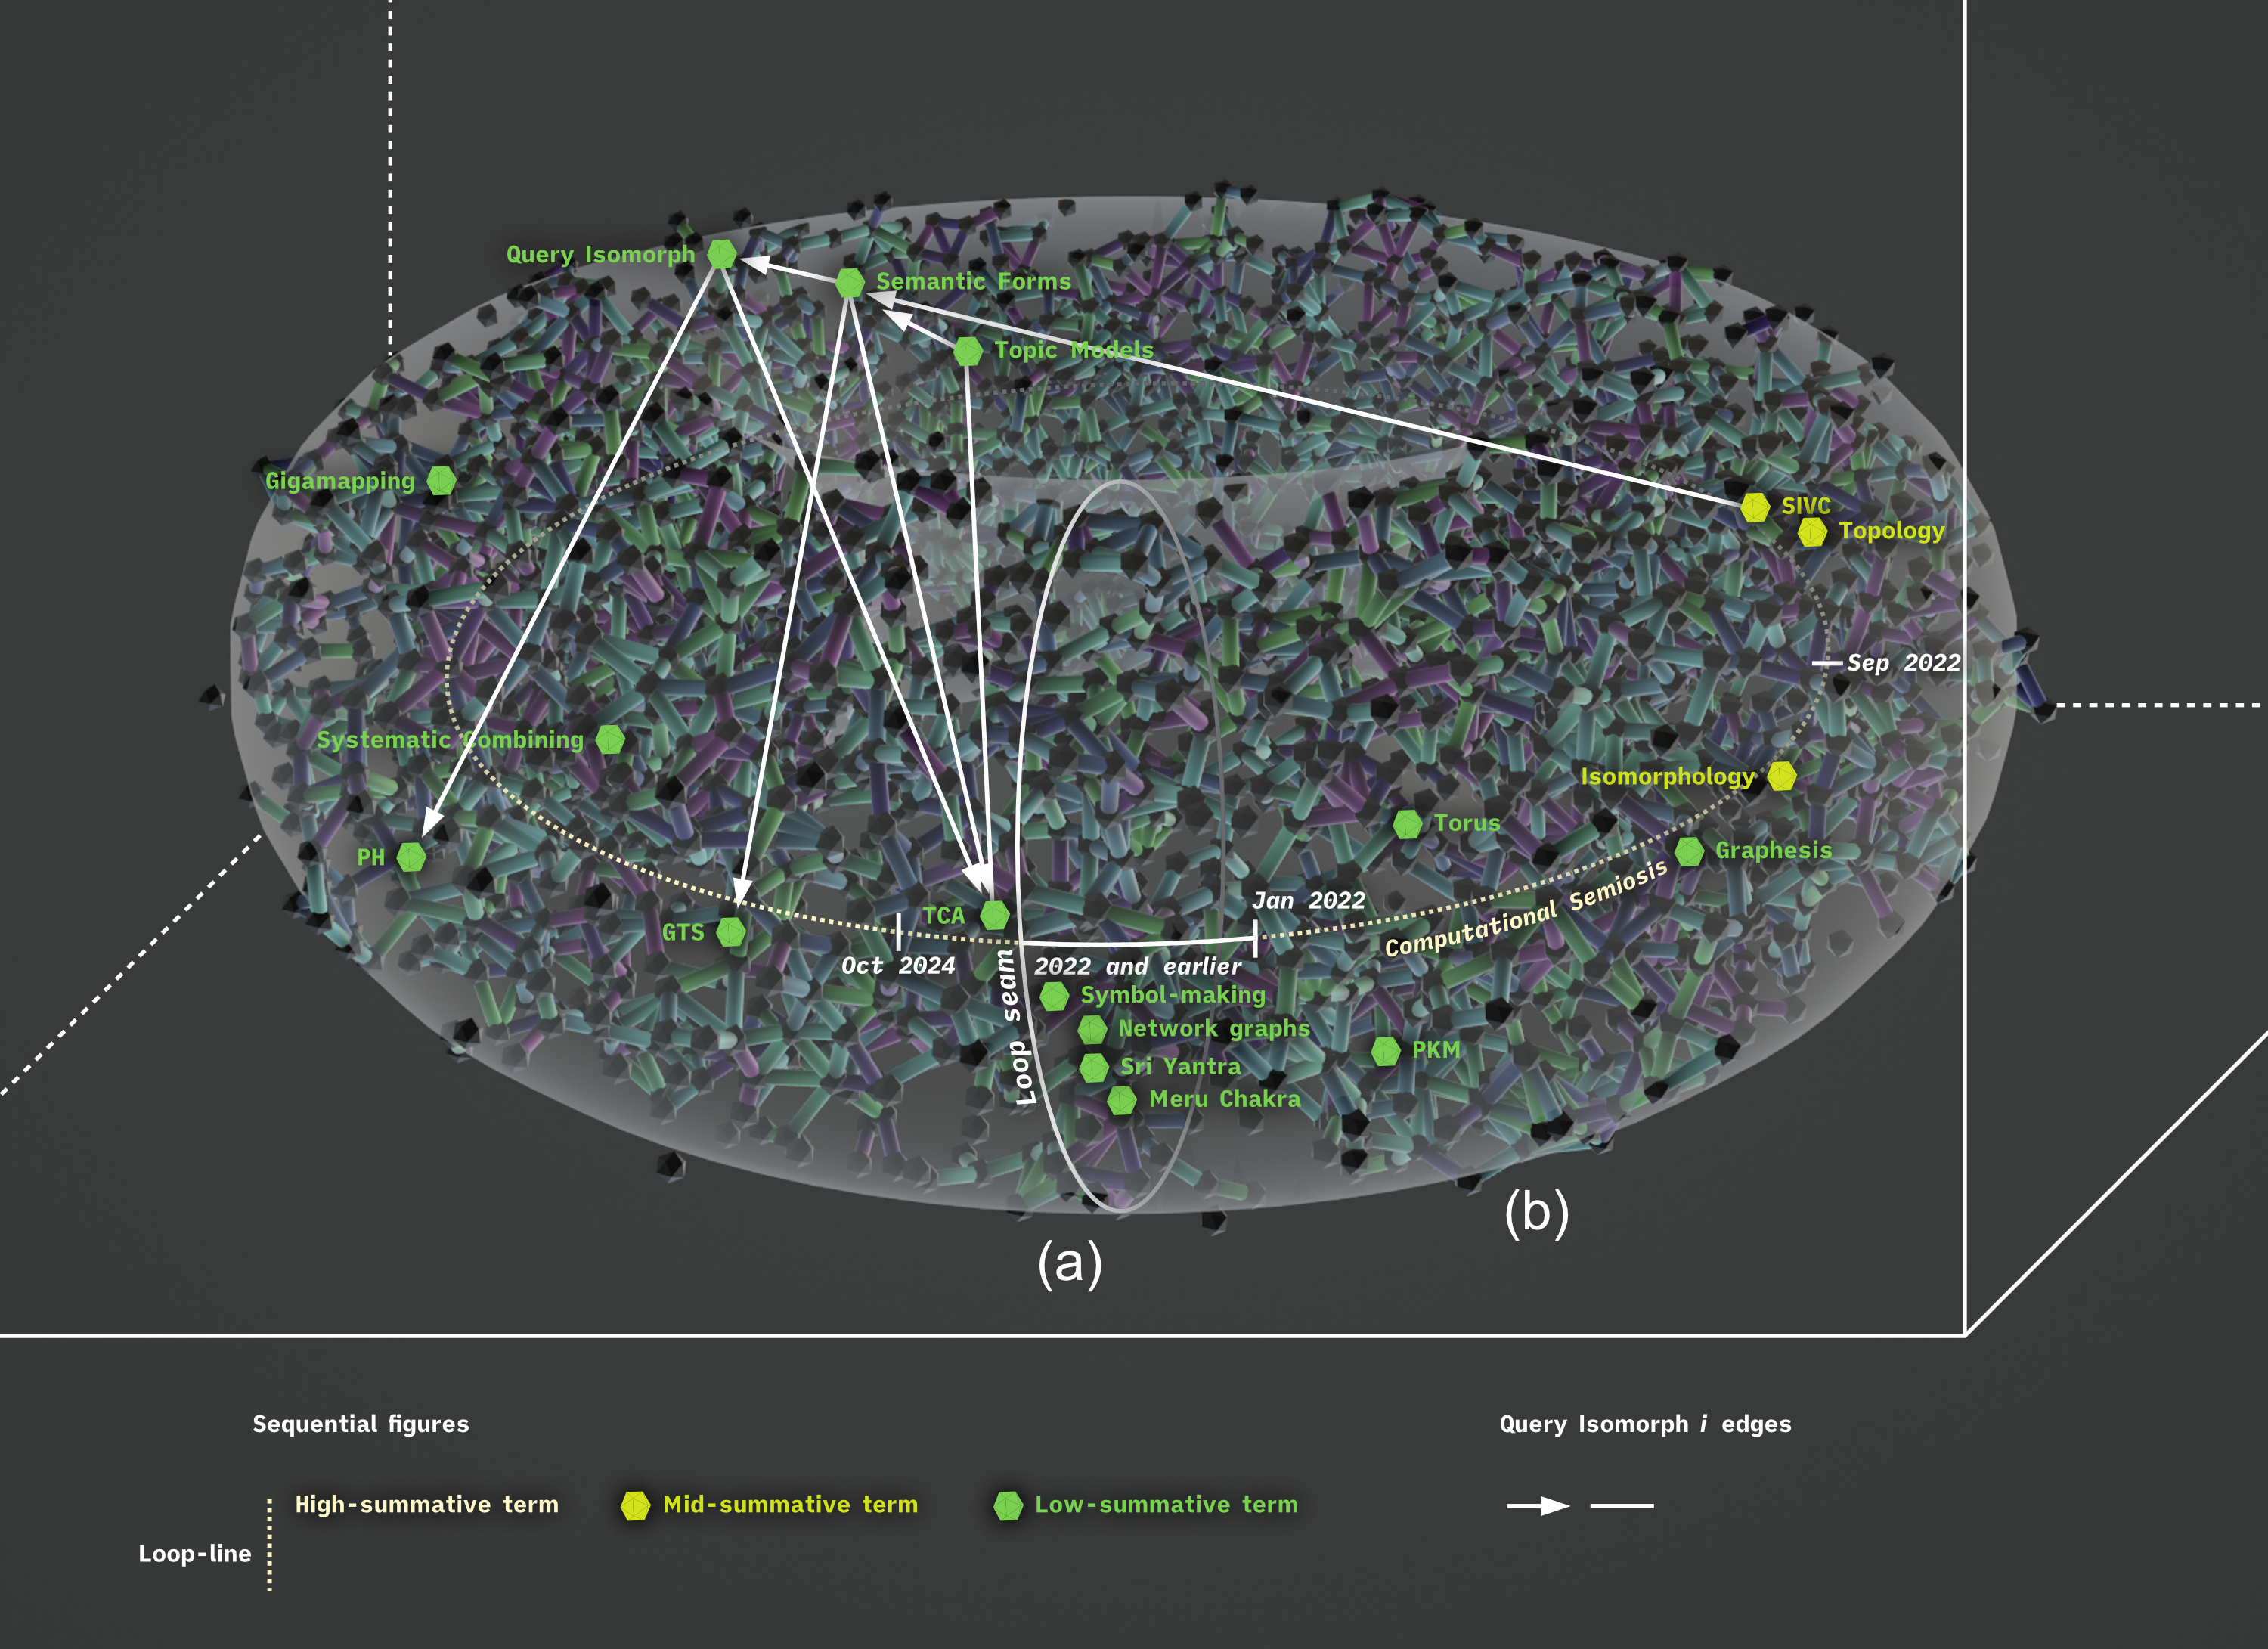
\includegraphics[width=\textwidth]{figures/5.12.RT1.png}
    \caption[Ring Torus Semantic Form about Query Isomorph \textit{i} with rectilinear edges]
    {\textbf{Ring Torus Semantic Form about Query Isomorph \textit{i} with rectilinear edges.} (a) is the Loop seam, and (b) is the Loop-line. Sample \textit{s} terms included for context.}
    \label{f5.12.RT1}
\end{figure}
\index[terms]{Ring Torus Semantic Form}
\FloatBarrier
\index[terms]{torus}

The following figures of Semantic Forms in this series of anticipatory renders of TCA Workspace will contextualize the spatial reconfiguration of Query Isomorph \textit{i} by including term-node pairings of Sample \textit{s}.

I visualized the warp of input Query Isomorph \textit{i} in the output Ring Torus Semantic Form in two ways: In \autoref{f5.12.RT1} I illustrated Query Isomorph edges using rectilinear edges to emphasize the derivation of each Query Isomorph \textit{i} node. In \autoref{f5.12aRT2}, I illustrated the Query Isomorph edges using long arcs that align with the curvature of the Ring Torus. This second style of edges emphasizes the sequence of each Query Isomorph \textit{i} node along the elliptical timeline. I anticipate that toggling between both options will be valuable in the Ring Torus Semantic Form, the Horn Torus Semantic Form, and any future Semantic Forms that involve curved plotting. 
\index[terms]{torus}

\autoref{f5.12.RT1} a) indicates the Loop Seam between the earliest dates and the latest dates along the timeline circle. Dates from Sample \textit{s} that were dated as “2022 and earlier” are labelled in a time segment to the right of the Loop Seam and left of “Jan 2022”. In the case of the Ring Torus Semantic Form, the through-line circles back into itself in what I am calling a Loop-line, indicated in \autoref{f5.12.RT1} b). The Loop-line represents a theme or themes that are both strongly present in a TCA database within a given time range and are expected to be perpetuated if existing semantic patterns continue. 

A computational method to query for topics that act as through-lines about a Query Isomorph in a Ring Torus Semantic Form would accelerate the analysis of texts and text groups. Similar functionality using OpenAI’s GPT-4 to name the relationship between nodes on a graph is already technologically possible, as shown earlier in a discussion about InfraNodus. To apply the Ring Torus Semantic Form, a researcher querying for through-lines using a ring-torus Semantic Form diagram could use this model to identify which topics in a given text most facilitate the continuation of a given thematic cycle.
\index[terms]{torus}


\FloatBarrier
To determine accurate node placement within the Ring Torus Semantic Form, I overlaid \autoref{f5.11.Time circle} as a guide. Specifically, I warped \autoref{f5.11.Time circle} so that its circumference matched the core line running through the Ring Torus in \autoref{f5.12.RT1}. I then moved each node manually along the radii lines of the superimposed and warped \autoref{f5.11.Time circle} either closer to the inner radius or outer radius of the ring torus, depending on my arbitrary measurement of how summative each term is. This technique aligns with the way PKM graphs position nodes by placing more highly connected nodes toward the middle. 
\begin{figure}[h!]
    \centering
    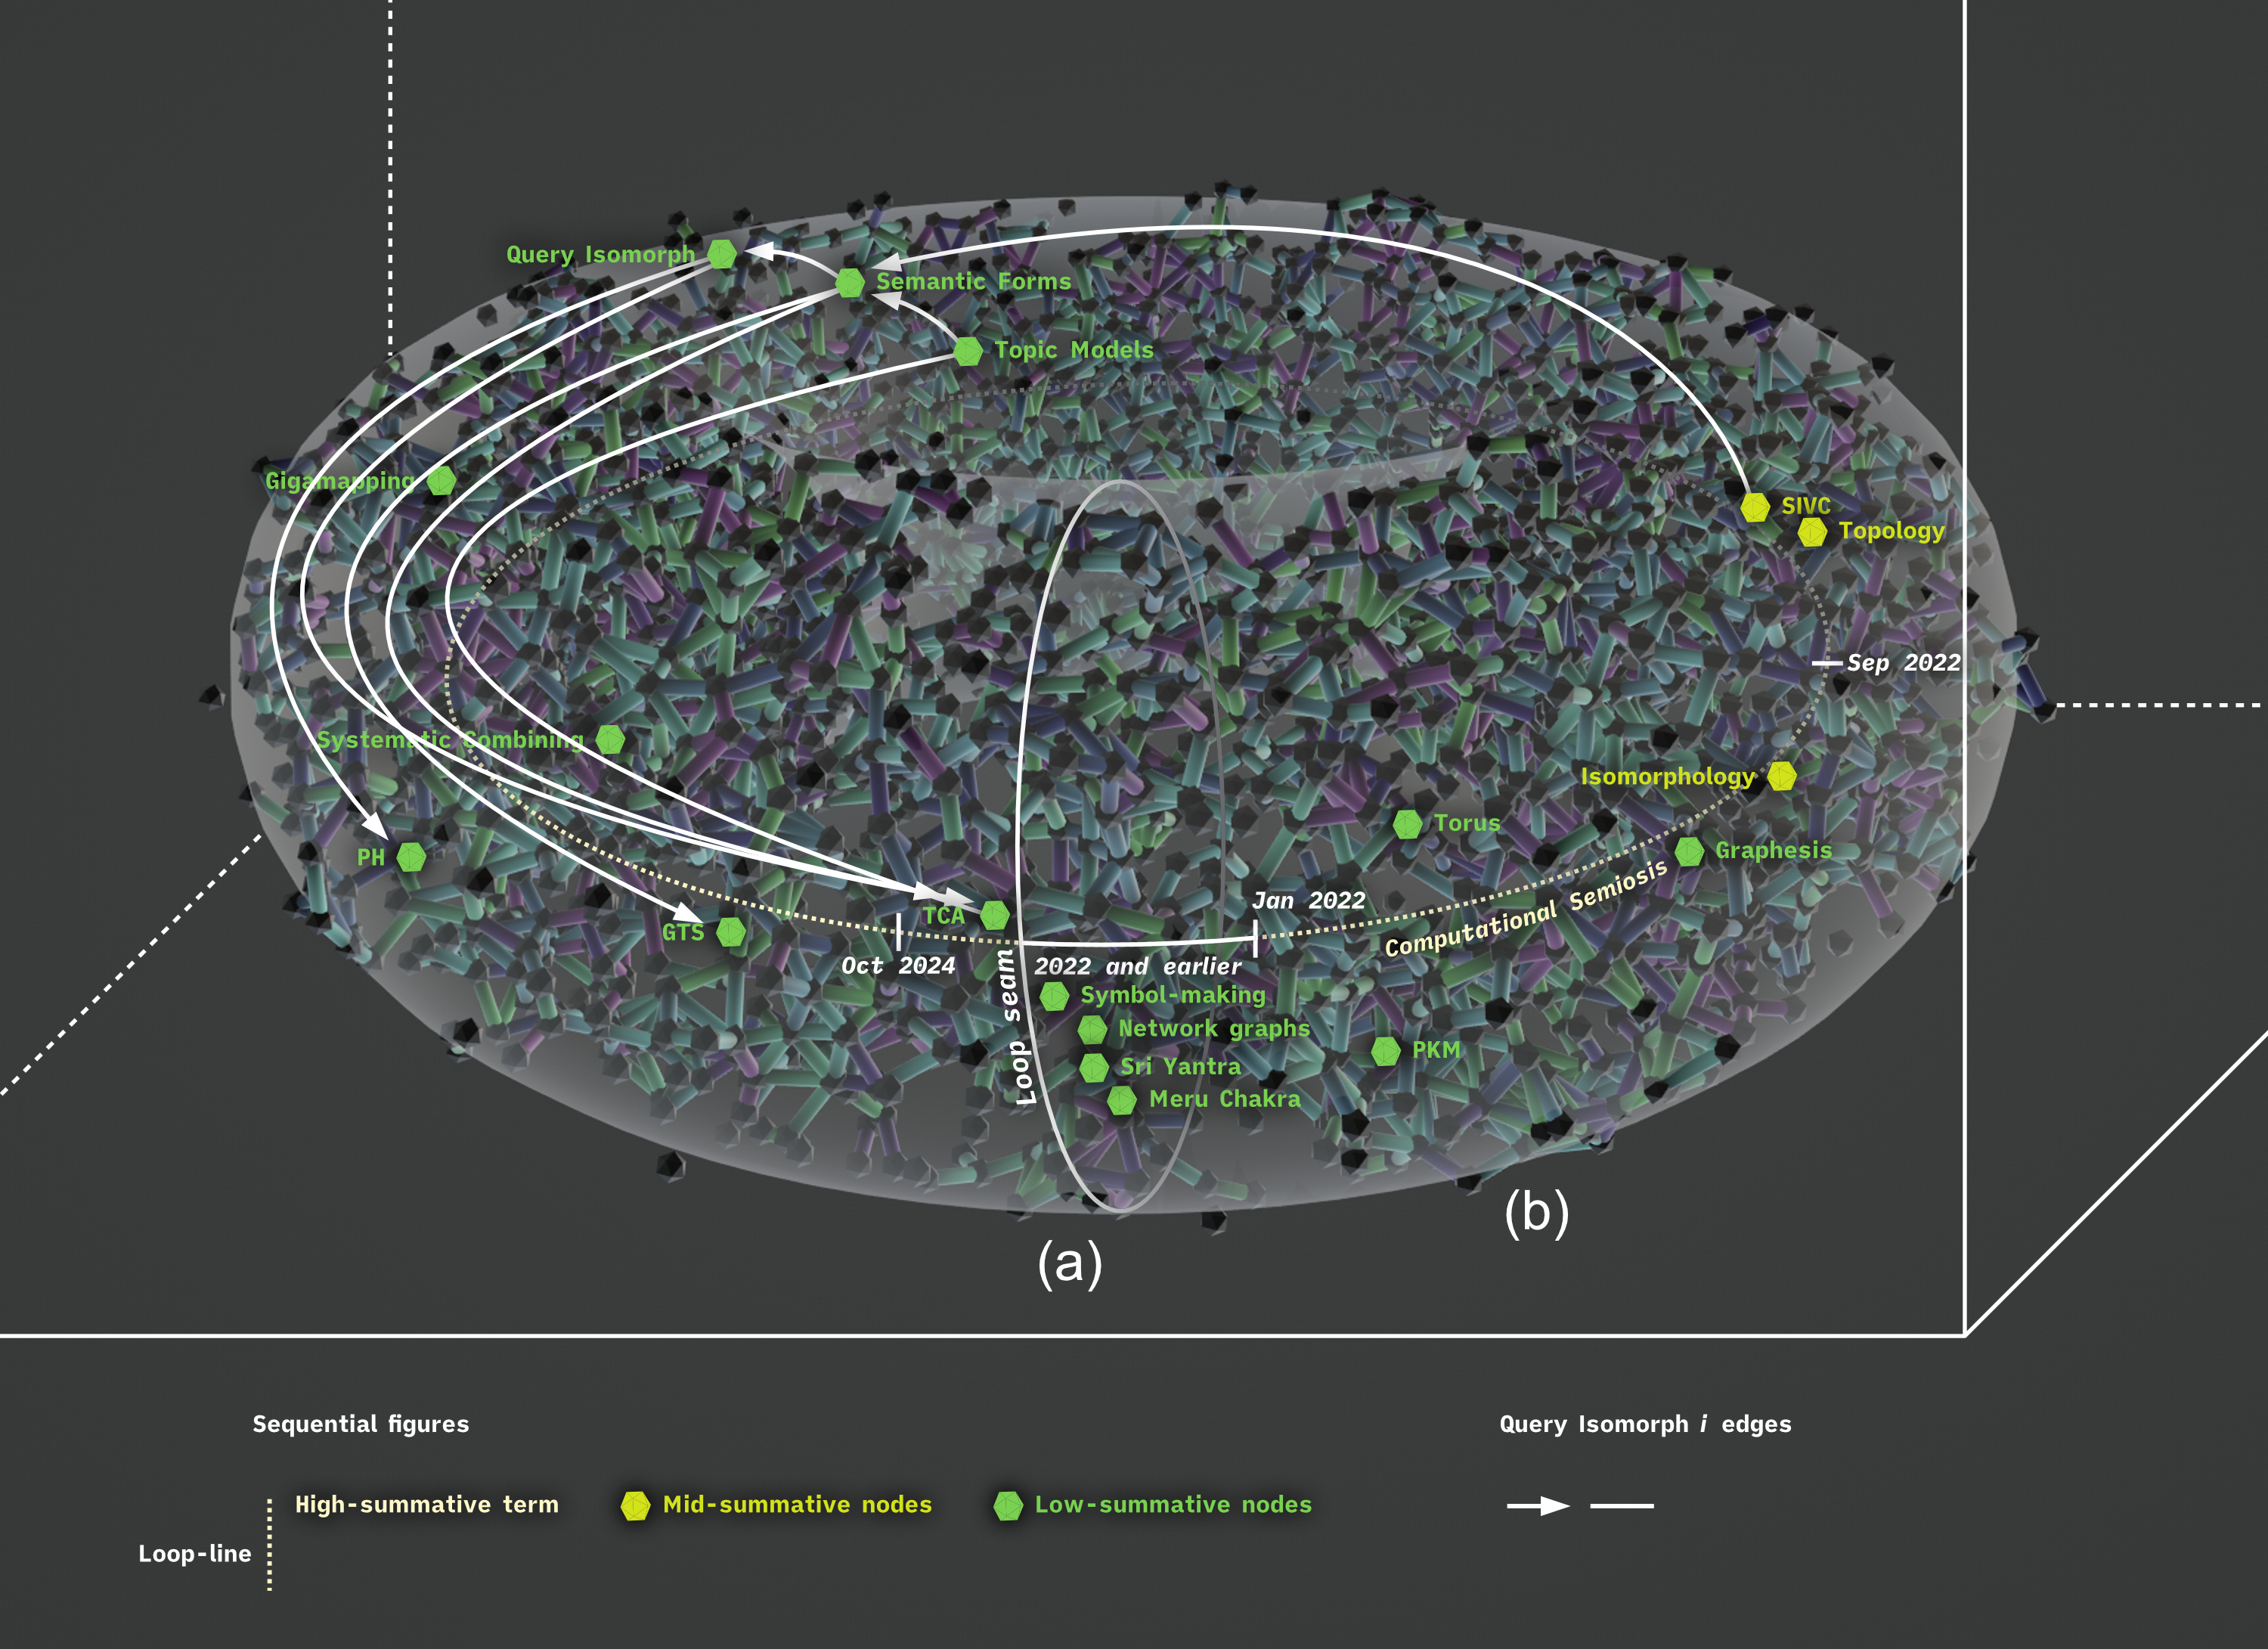
\includegraphics[width=\textwidth]{figures/5.12aRT2.png}
    \caption[Ring Torus Semantic Form about Query Isomorph \textit{i} with arced edges]
    {\textbf{Ring Torus Semantic Form about Query Isomorph \textit{i} with arced edges.} (a) is the Loop seam, and (b) is the Loop-line. Sample \textit{s} terms included for context.}
    \label{f5.12aRT2}
\end{figure}
\index[terms]{Query Isomorphs}
\FloatBarrier  

\clearpage


\subsubsection{Query Isomorph \textit{i} in the Cone and Double Cone Semantic Forms}

\paragraph{Cone Semantic Form} \mbox{} \\

\begin{figure}[h!]
    \centering
    \includegraphics[width=\textwidth]{figures/5.13.Cone.png}
    \caption[Cone Semantic Form about Query Isomorph \textit{i}]
    {\textbf{Cone Semantic Form about Query Isomorph \textit{i}. }Sample \textit{s} terms included for context.}
    \label{f5.13}
\end{figure}
\FloatBarrier  


As opposed to chronological sequence captured in the Cylinder and Ring Torus Semantic Forms, I doubly encode node summativeness in the Cone Semantic Form  using colour and placement. Highly summative nodes are hued light yellow or yellow and placed closer to the Cone's peak, while mid-summative or low-summative nodes are hued green and placed in the middle of the cone or toward its base. Query Isomorph \textit{i} is labelled by connecting its nodes with white edges. 

%Applies to the Ontological Semantic Network Summaries in that the terms which are fewer in number towards the top point are the most summative and have the most subsequent terms derived from them.

\index[terms]{Query Isomorphs}
\index[terms]{torus}
\index[terms]{Semantic Forms}
\index[terms]{Ontological Semantic Network Summaries (OSNS)}
\FloatBarrier


\clearpage

\paragraph{Double Cone Semantic Form} \mbox{} \\


\begin{figure}[h!]
    \centering
    \includegraphics[width=\textwidth]{figures/5.14.DoubleCone.png}
    \caption[Double Cone Semantic Form about Query Isomorph \textit{i}]{\textbf{Double Cone Semantic Form about Query Isomorph \textit{i}.} Sample \textit{s} terms included for context.}
    \label{f5.14.DoubleCone}
\end{figure}
\index[terms]{Query Isomorphs}
\FloatBarrier  

Using the Double Cone Semantic Form, I represent deduction and induction using node divergence and convergence, respectively. Building off the node group label style of InfraNodus \citep{paranyushkin_infranodus_nodate-2}, I hue Theology terms in purple, Semiosis terms in Orange, and 3D information visualization composition terms in Teal, and Graph Math terms in Magenta. My design of the Double Cone Semantic Form follows important precedents; as traced by Sevaldson \citep[p. 102]{sevaldson_designing_2022}, these include Pappus (290-350) \citep[p. 7]{hinitikka_method_1974}, Bánáthy’s model \textit{The dynamics of divergence and convergence} \citep[p. 75]{banathy_designing_1996}, and the British Design Council's Double Diamond framework \citep{design_council_history_nodate}. However, my Double Cone Semantic Form methodological proposal differs from these precedents visuospatializing past two dimensions, applicably to HATG and TCA in HITL CATG.


\index[people]{Sevaldson, Birger}
\index[people]{Bánáthy, Béla Heinrich}
\index[people]{Pappus}


\subsubsection{Query Isomorph \textit{i} in the Sphere and Horn Torus Semantic Forms}

\FloatBarrier


\paragraph{Sphere Semantic Form} \mbox{} \\


\begin{figure}[h!]
    \centering
    \includegraphics[width=\textwidth]{figures/5.15.Sphere1.png}
    \caption[Sphere Semantic Form about Query Isomorph \textit{i}]
    {\textbf{Sphere Semantic Form about Query Isomorph \textit{i}.} This Sphere Semantic Form contains three Cone Semantic Forms: (a) which is about Spatial Information Visualization Composition and Isomorphology, (b) which is about text graph methods of visuospatial knowledge production, and (c) which is about Topology. Sample \textit{s} terms included for context.}
    \label{5.15.Sphere1}
\end{figure}
\index[terms]{Query Isomorphs}
\FloatBarrier  

The Sphere Semantic Form is similar to the Cone Semantic Form in that it represents hierarchical relationships between nodes. However, while the Cone Semantic Form can represent various hierarchies within itself, it predominantly represents one hierarchy. The Sphere Semantic Form effectively represents multiple cone semantic forms, increasing the number of hierarchies that can be represented. 
\index[terms]{Semantic Forms}

\autoref{5.15.Sphere1} illustrates how the high-summative node Computational Semiosis is shared by three Cone Semantic Forms: (a) which is about Spatial Information Visualization Composition and Isomorphology, (b) which is about text graph methods of visuospatial knowledge production, and (c) which is about Topology.  
\index[terms]{topology}
\index[terms]{Semantic Forms}
\index[terms]{Spatial Information Visualization Composition (SIVC)}
\index[terms]{isomorphology}

I present the Sphere Semantic Form with nested Cone Semantic Forms to illustrate an additional notation method for grouping nodes that does not depend on colour encoding like in \autoref{f5.14.DoubleCone}, which increases the researcher's ease of interpretation and avoids opportunities for accessibility issues related to colour blindness. In the same way that the Circle Semantic Shape can contain and overlap with Triangle and Circle Semantic Shapes, like in the Obsidian knowledge graph in \autoref{f5.2}, the Sphere Semantic Form can nest and overlap with Cone and Sphere Semantic Forms. The number of nodes that can be organized in nested hierarchies of Semantic Forms is substantially more than the nodes that can be represented in a Circle Semantic Shape due to their dimensional difference. I expect that testing user experience of reading node hierarchies in Semantic Forms versus Semantic Shapes will reveal results consistent with Ware and Mitchell's \textit{Visualizing graphs in three dimensions} \citep[p. 10]{ware_visualizing_2008} in which users will be able to benefit significantly from a three-dimensional interface for dense graphs.
\index[terms]{Semantic Forms}
\clearpage

\FloatBarrier


\paragraph{Horn Torus Semantic Form} \mbox{} \\

\begin{figure}[h!]
    \centering
    \includegraphics[width=\textwidth]{figures/5.16.HT2.png}
    \caption[Horn Torus Semantic Form about Query Isomorph \textit{i}]
    {\textbf{Horn Torus Semantic Form about Query Isomorph \textit{i}.} Sample \textit{s} terms included for context.}
    \label{f5.16.HT2}
\end{figure}

\index[terms]{Query Isomorphs}
\FloatBarrier  

The Horn Torus Semantic Form is similar to the Ring Torus and Cylinder Semantic Forms in that it represents a series of Circle Semantic Shapes, like a Rolodex \citep{mellby_my_2021} of Obsidian or Logseq graphs in one continuous space as the tube of its body. However, the inner radius of the Ring Torus narrows to a single highly-summative point in the centre of the Horn Torus Semantic Form, making two Cone Semantic Forms which diverge away from each other as negative space outside the Horn Torus. Furthermore, the Loop-line of the Ring Torus Semantic Form is a Zone of Semantic Stasis in the Horn Torus Semantic Form, where ideas are the most consistent and unchanging.

I oriented my model Horn Torus Semantic Form to dimple above and below to evoke trees. The core of the torus represents the trunk which branches up and out, whose leaves fall and transform into the soil, whose nutrients are taken up by the tree's roots–represented by the bottom horn torus dimple. These nutrients are taken back into the tree to the trunk re-origin point in an ongoing cycle of blossoming transformation representative of ideas' flux.
\index[terms]{torus}
\index[terms]{Semantic Forms}

I depict these Horn Torus Semantic Form trajectories of transformation as arcs emerging and returning to their re-origin point. Similarly to the Ring Torus, I used \autoref{f5.11.Time circle} to accurately place term nodes from semantic field \textit{S} with chronological precision onto their respective arcs. The re-origin point, Computational Semiosis, is in the high-summative sequential figure colour light yellow. I depicted the transformation trajectory arcs by labelling them in categorical figure colours: the Semantic Forms arc in Teal, the Query Isomorph arc in Magenta, and the TCA Platform arc in Orange. My transformation trajectory arcs follow the circumference of the torus tube like Rucker's vertical arc orbits representing time in his horn torus model of space-time \citep{rucker_infinity_2005}. However, my transformation trajectory arcs blossom upward and out from the horn torus's centre.
\index[terms]{torus}
\index[terms]{horn torus}
\index[terms]{Semantic Forms}

The Horn Torus Semantic Form differs from the Sphere Semantic Form because it does not nest a variety of Cone Semantic Forms within it at different angles. In fact, the two Cone Semantic Forms at the poles of the Horn Torus Semantic Form represent Gestaltian geometric liminality and interbeing \citetext{\citealp[p. 25]{deleuze_thousand_2007}; \citealp[p. 81-82]{nhat_hanh_world_2008}} of Semantic Form in which the Cone Semantic Form and the Ring Torus Semantic Form are exactly at the brink of being their own forms, being each other, and being a whole that ``is other than the sum of its parts."  \citep[Koffka in Sevaldson, p. 163]{sevaldson_designing_2022}. This thesis is, in many ways, a celebration of the strange and wonderful qualities of the horn torus as a spatial information visualization composition, particularly as a network graph isomorph.
\index[people]{Sevaldson, Birger}
\index[terms]{torus}
\index[terms]{horn torus}
\index[people]{Thích Nhất Hạnh}
\index[people]{Deleuze, Gilles}
\index[people]{Guattari, Félix}
\index[terms]{Semantic Forms}
\index[terms]{Spatial Information Visualization Composition (SIVC)}


\FloatBarrier  
\begin{figure}[h!]
    \centering
    \includegraphics[width=\textwidth]{figures/5.17.HT3.png}
    \caption[Horn Torus Semantic Form about Query Isomorph \textit{i} dimensionally reduced to 2D]
    {\textbf{Horn Torus Semantic Form about Query Isomorph \textit{i} dimensionally reduced to 2D.} Sample \textit{s} terms included for context.}
    \label{f5.17.HT3}
\end{figure}
\FloatBarrier  
\index[terms]{torus}
\index[terms]{Query Isomorphs}




In \autoref{f5.17.HT3} I illustrate two sequences of Horn Torus Semantic Form re-origination in a dimensional \textit{reduction} of \autoref{f5.16.HT2}. On the left, I represent the research before my graduate work at OCAD U in a cycle of divergence and convergence. To the right, I represent my thesis research at OCAD U, which leads to future work. I represent  Query Isomorph \textit{i} by connecting its nodes with white colour edges. The three transformation trajectory arcs from \autoref{f5.16.HT2} are included, but left of the bracket for Thesis research, I added arcs to represent a rough timeline of encountering key formative ideas that preceded my work at OCAD U. First, I added a Theological arc, which includes the terms Theology, Sacred geometry, Vedic meditation, Sri Yantra, and Torus. Note here that the Torus is included earlier in this representation because my fascination with it began with artistic representations of chakras as horn tori. Also, note that the Meru Chakra is placed directly before the beginning of my thesis research arcs and directly before Network graphs. I labelled the Theology arc Purple, the Semantic Forms arc Teal, and the Query Isomorphs arc Magenta because I arrived at a study of network graphs through my fascination with the Meru Chakra. Since the development of Semantic Forms and Query Isomorphs are distinct extensions and disambiguations of a theological principle, I used colour to represent how the Teal Semantic Forms arc and the Magenta Query Isomorphs arc are the separation of blue and red primary colours that make up Purple. Second, the TCA Platform arc extends backward into a short origin story, including Note-taking methods, Mind mapping  \citep{buzan_ultimate_2005}, and Symbol-making. Both arcs and additions left of my Thesis research arcs represent a rough timeline, as I mentioned. I spread each idea along the timeline according to my estimated age when I encountered each idea. The nodes furthest left on the timeline represent the earliest ideas that influenced this research, and the nodes closest to the beginning of my thesis research arcs represent the ideas that were most influential right before beginning my degree at OCAD U. 
\index[terms]{torus}
\index[terms]{Query Isomorphs}
\index[terms]{Semantic Forms}

\clearpage


        

\section{Contribution 7. TCA Workspace, for living webs of thought}
\FloatBarrier  
\begin{enumerate}
      \item[\textbf{C7}] \textit{TCA Workspace}, a methodological prototype of a collaborative HITL CATG + HATG platform to:
    \begin{enumerate}
        \item[(a)] integrate all my thesis contributions (\textit{Semantic Forms}, \textit{Query Isomorphs}, \textit{OSNS}, \textit{Symbol-setting}, \textit{TTG}, and \textit{TCA Researcher Grouping}).
        \item[(b)] facilitate computational interface with Systemic Design methods for visuospatial reasoning encountered through my literature review, such as gigamapping \citetext{\citealp{sevaldson_giga-mapping_2011}; \citealp[p. 26]{sevaldson_designing_2022}} and Systematic Combining \citetext{\citealp[p. 554]{dubois_systematic_2002}; \citealp{kjode_entanglement_2024}}.
    \end{enumerate}
\end{enumerate}
\FloatBarrier  
\index[terms]{Systemic Design}
\index[terms]{gigamapping}
\index[terms]{Systematic Combining (SC)}
\index[terms]{TCA Researcher Grouping}
\index[terms]{Semantic Forms}


TCA Workspace is my proposal for a software platform which will accelerate the computational analysis of texts and graphs with Semantic Forms, Query Isomorphs, Symbol-setting, Ontological Semantic Network Graphs, and Terroir of Text and Graphs (TTG) as independent tools or as combined approaches. The ‘space’ in TCA Workspace invokes the dimensionality of ‘place’ as well as the colliding of electromagnetic particles in nested holarchies of complexity, from the atoms that are our words to the ontologies that are our visible universes. In this sense, TCA Workspace would be a particle accelerator of ideas that activates living webs of thought.
\index[terms]{TCA Workspace}
\index[terms]{Terroir of Text and Graphs (TTG)}
\index[terms]{Symbol-setting}
\index[terms]{Query Isomorphs}




In TCA Workspace, researchers would identify and examine isomorphogenic molecular dynamics simulations of `datacules’, formed of spatial network graphs of entities and relationships in Query Isomorphs and Semantic Forms. Researchers would be able to identify and observe the semantic forces at play in text and graphs, using the rich visuospatial analogues available from across the sciences and humanities, and use computational Topological Capta Analysis. The identification of semantic structures and `datacules' will build on computational chemistry, including the Nobel prize-winning work of David Baker, Damis Hassabis, and John Jumper \citep{jumper_highly_2021,krishna_generalized_2024,the_royal_swedish_academy_of_sciences_press_2024}. Anticipating and developing interdisciplinary methods like the ones proposed in my thesis can be a means of identifying and leveraging latent Sustainability Transitions solutions in the visuospatial meta-patterns of knowledge production.
\index[terms]{TCA Workspace}
\index[terms]{Query Isomorphs}
\index[terms]{Semantic Forms}
\index[terms]{Topological Capta Analysis (TCA)}


In the following sections I invite the consideration of how current approaches to graphs and text are aligned with and can be expanded by the TCA Workspace toolkit.

\subsection{Dimensional addition in Systems Oriented Design with Semantic Forms and Query Isomorphs}
Considering the Meta-Systematic Combining approach I used in this thesis for arriving at Semantic Forms through dimensional addition of Semantic Shape, I propose dimensional addition to Sevaldson’s gigamaps \citep{sevaldson_giga-mapping_2011,sevaldson_designing_2022} as a feature of TCA Workspace that can work concurrently with Semantic Forms and Query Isomorphs. As introduced in \autoref{f5.9.Semantic Shape Circle} with the spatial TCA Workspace representation of the Circle Semantic Shape PKM graph with an overlay of Query Isomorph nodes, I do not intend to represent information in only two-dimensions or three-dimensions in TCA Workspace; instead, I think both can be valuable together in the same render. To illustrate the dimensional versatility of the interface of TCA Workspace, I present two examples of visuospatial gigamaps: \autoref{f5.30.HT gig} my Horn Torus Semantic Form gigamap and \autoref{f5.31.Cone gig} my Cone Semantic Form gigamap.
\index[people]{Sevaldson, Birger}
\index[terms]{Query Isomorphs}
\index[terms]{Systems Oriented Design (SOD)}
\clearpage


\FloatBarrier  
\subsubsection{Gigamaps with Semantic Forms}
\index[terms]{Semantic Forms}


\paragraph{Horn Torus Semantic Form gigamap} \mbox{} \\
\begin{figure}[h!]
    \centering
    \includegraphics[width=0.8\textwidth]{figures/5.30.HT gig.png}
    \caption[Horn Torus Semantic Form gigamap]{\textbf{Horn Torus Semantic Form gigamap.} The spatial network graph in the middle is dimensionally reduced into two-dimensional panes a, b, and c: (a) and (b) reveal the Disintegration and Integration arcs from \autoref{f4.1} which organize the semantic relationships of divergence and convergence from \autoref{f5.16.HT2}. (c) depicts the top view of this Horn Torus Semantic Form as a Mind Map \citep{buzan_ultimate_2005}. Sample \textit{s} terms included for context.}
    \label{f5.30.HT gig}
\end{figure}
\FloatBarrier  
\index[terms]{torus}

In \autoref{f5.30.HT gig}, I depict a conceptual gigamap of a spatial Horn Torus Semantic Form network graph and a sample of dimensional reduction viewing panes. Panes (a) and (c) are depicted as revealing the Disintegration and Integration arcs from \autoref{f4.1} and \autoref{f5.16.HT2}. Pane (b) represents dimensional reduction to a Circle Semantic Shape, in this case as a Mind Map \citep{buzan_ultimate_2005}. The panes' perpendicular angles were chosen for simplicity of introduction, but pane angles would vary widely. Surveying a Semantic Form network graph using multiple angles of dimensionality reduction, algorithmically or not, could reveal significant node correlations that would otherwise be missed. 
\index[terms]{torus}
\clearpage

\FloatBarrier  

\paragraph{Cone Semantic Form gigamap} \mbox{} \\
\begin{figure}[h!]
    \centering
    \includegraphics[width=0.8\textwidth]{figures/5.31.Cone gig.png}
    \caption[Cone Semantic Form gigamap about Query Isomorph \textit{i}]
    {\textbf{Cone Semantic Form gigamap about Query Isomorph \textit{i}.} The network graph is dimensionally reduced in four angles into two-dimensional panes: (a) in a Cone of Plausibility \citep{bezold_overview_1993}, (b) as an inductive and deductive reasoning analysis, (c) as a Horn of Futures model, and (d) as an adaptation of “Diagram of a design process with iterations” \citetext{\citealp[p. 343]{sevaldson_designing_2022}; \citealp{sevaldson_designing_2022-1}}. Sample \textit{s} terms included for context.}
    \label{f5.31.Cone gig}
\end{figure}
\FloatBarrier  

Second, I depict a conceptual gigamap with a Cone Semantic Form network graph dimensionally reduced in four angles: (a) in a Cone of Plausibility \citep{bezold_overview_1993}, (b) as an inductive and deductive reasoning analysis, (c) as a Horn of Futures model, and (d) as an adaptation of “Diagram of a design process with iterations” \citetext{\citealp[p. 343]{sevaldson_designing_2022}; \citealp{sevaldson_designing_2022-1}}, similarly to \autoref{f5.30.HT gig}, these angles are not prescriptive to the practice of Cone Semantic Form gigamapping. 
\index[people]{Bezold, Clement}
\index[people]{Sevaldson, Birger}
\clearpage

\subsubsection{Systematic Combining with Semantic Forms and Query Isomorphs}
Systematic Combining (SC) is a form of Knowledge Production that combines diagrams into larger, more integrated, and capacious models. The driving urgency of my work is Sustainability Transitions, so I examine the doctoral thesis and Systematic Combinations of Svein Gunnar Kjøde, \textit{Entanglement of Systemic Design and Sustainability Transitions} \citep{kjode_entanglement_2024}, as a case study for the existing use of Spatial Information Visualization Composition (SIVC) in Design for Sustainability Transitions. Identifying the current use of SIVC is valuable to me because it demonstrates areas that would benefit from the key functions of TCA Workspace, such as Semantic Forms and Query Isomorphs. 
\index[people]{Kjøde, Svein Gunnar}
\index[terms]{Query Isomorphs}
\index[terms]{Spatial Information Visualization Composition (SIVC)}

I found that Kjøde included or made SIVCs using three geometric forms, which are among my six Semantic Forms, represented in \autoref{f5.23}, \autoref{f5.25},  \autoref{f5.27}. First, the sphere, which organizes the ideas in \autoref{f5.23} the “Floke programme and quadruple helix for stakeholder inclusion” \citep[p. 125]{kjode_entanglement_2024}. Second, the cone, which organizes the ideas in \autoref{f5.25}, Kjøde’s “Relating systemic design practice to socio-technical systems theory and the MLP” \citep[p. 123]{kjode_entanglement_2024}. Third, the cylinder which organizes the ideas in \autoref{f5.27}, Kjøde’s “Praxeological framework for DfST relating to systematic transition initiatives” \citep[p. 144]{kjode_entanglement_2024}. The first two figures have a more self-evident similarity to my Semantic Forms. The third figure, \autoref{f5.27}, is a four-lobed visualization with the words “Systemic Praxeology of DfST” in its centre. This four-lobed figure is indicated to occupy the one-dimensional “Systemic Practice”, which is labelled as a colourful double-directional arrow pointing from the bottom left to the top right. “Systemic Practice” is labelled as one ‘slice’ of a cylindrical spiral labelled with a single-directional arrow and the words “Transition Initiative(s).” To apply my terminology as a summation, Kjøde’s four-lobed “Systemic Praxeology of DfST” is a two-dimensional Circle Semantic Shape in a Cylinder Semantic Form, similar to the composition of \autoref{f5.10.Cylinder} which represents a cylinder of PKM graphs. 
\index[people]{Kjøde, Svein Gunnar}

To relate my work to Kjøde’s, I include a fourth figure, \autoref{f5.28.Kjode b}, which represents how nodes in Sample \textit{s} and Query Isomorph \textit{i} would be positioned in relation to “Systemic Praxeology of DfST” \citep[p. 144]{kjode_entanglement_2024}. This four-lobed form operates similarly to a Circle Semantic Shape, so I place terms with higher summativeness toward the figure’s centre.
\index[people]{Kjøde, Svein Gunnar}
\index[terms]{Query Isomorphs}

\FloatBarrier  
\begin{figure}[h!]
    \centering
    \includegraphics[width=0.5\textwidth]{figures/5.23.png}
    \caption[Spherical SIVC in DfST]
    {\textbf{Spherical SIVC in DfST.} This figure is based on the ``Floke programme and quadruple helix for stakeholder inclusion” in Kjøde \citep[p. 125]{kjode_entanglement_2024}
}
    \label{f5.23}
\end{figure}
\index[people]{Kjøde, Svein Gunnar}

\begin{figure}[h!]
    \centering
    \includegraphics[width=0.5\textwidth]{figures/5.25.png}
    \caption[Conical SIVC in DfST]
    {\textbf{Conical SIVC in DfST.} This figure is based on Kjøde’s ``Relating systemic design practice to socio-technical systems theory and the MLP” \citep[p. 123]{kjode_entanglement_2024}. This figure includes Norwegian terms left of ``Sustainability Transitions” to indicate the ``patchwork of regimes” in overlapping aspects of ``Socio Technical Change”: utbygging, drift, rehabilitering, sanering, and gjenbruk: Utbygging refers to the initial ``development” \citep{cambridge_university_press_utbygging_nodate}; Drift refers to the ongoing operations and management \citep{cambridge_university_press_drift_nodate}; Rehabilitering refers to the ``rehabilitation” or restoration and upgrading of existing structures  \citep{cambridge_university_press_rehabilitering_nodate}; Sanering refers to ``clearing” or sanitation \citep{cambridge_university_press_sanering_nodate-3}; Gjenbruk refers to reusing or recycling \citep{cambridge_university_press_gjenbruk_nodate}.
}
    \label{f5.25}
\end{figure}
\index[people]{Kjøde, Svein Gunnar}




\begin{figure}[h!]
    \centering
    \includegraphics[width=\textwidth]{figures/5.27.png}
    \caption[Cylindrical SIVC in DfST]
    {\textbf{Cylindrical SIVC in DfST.} This figure is based on Kjøde’s ``Praxeological framework for DfST relating to systematic transition initiatives” \citep[p. 144]{kjode_entanglement_2024}.
}
    \label{f5.27}
\end{figure}
\index[people]{Kjøde, Svein Gunnar}



\begin{figure}[h!]
    \centering
    \includegraphics[width=\textwidth]{figures/5.28.Kjode b.png}
    \caption
        [Kjøde's DfST Systematic Combining gigamap visualized as Cylinder Semantic Form network graph with Query Isomorph \textit{i} and Sample \textit{s}]
        {\textbf{
            Kjøde's DfST Systematic Combining gigamap visualized as Cylinder Semantic Form network graph with Query Isomorph \textit{i} and Sample \textit{s}.} The portion of this figure which is \autoref{f5.27} is based on Kjøde’s ``Praxeological framework for DfST relating to systematic transition initiatives” \citep[p. 144]{kjode_entanglement_2024}. Sample \textit{s} terms included for context.
}
    \label{f5.28.Kjode b}
\end{figure}
\FloatBarrier  
\index[people]{Kjøde, Svein Gunnar}
\index[terms]{gigamapping}
\index[terms]{Systematic Combining (SC)}
\index[terms]{Query Isomorphs}





\FloatBarrier  
\subsubsection{LLM as Sphere Semantic Form}
\begin{figure}[h!]
    \centering
    \includegraphics[width=\textwidth]{figures/5.15.Sphere LLM.png}
    \caption[Sphere Semantic Form as LLM Vector Embeddings]
    {\textbf{Sphere Semantic Form as LLM Vector Embeddings.}
}
    \label{f5.15.Sphere LLM}
\end{figure}
\FloatBarrier  

Although LLMs can rely on graphs of text, such as vector embeddings, they are not intended as information visualization. For a model to be usable as AI, it seems to requires a high-dimensionality that embed thousands of dimensions. In this sense LLM vector graphs are beyond visuospatial representation. They cannot be seen or captured spatially, at least not without compromising the semantic value of its dimensional interrelationships by using dimensionality reduction.

I turn here to Grant Sanderon’s illustrations of vector space, which show how LLMs organize ideas as radii around a central origin point \citep{sanderson_attention_2024}. Vector embeddings operate as the direction of a line- or vector- in space, but individual node positions work differently. However, the specificity of a vector still allows for graphing individual coordinates, though variable, with the use of topology, which is less concerned with exact coordinates. Query Isomorphs may be compatible with the LM vector graph; for the sake of UI, Query Isomorphs may be input as individual points but searched along vector lines within an LM. In this way, the LM is an example of a Sphere Semantic Form and a prospect for using Query Isomorphs within texts or groups of texts. This treatment of LM vector graphs opens up interoperability with network graphs, and their spherical composition can be represented and leveraged as a Semantic Form.
\index[terms]{Language Model (LM)}
\index[terms]{Large Language Model (LLM)}
\index[terms]{topology}
\index[terms]{Query Isomorphs}



\subsubsection{Section conclusion}

I propose that by using Systematic Combining and other forms of Systemic Design in the Design for Sustainability Transitions (DfST), Kjøde and I are engaging in a Systemic Design for Sustainability Transitions (SDfST). However, building on Pangaro, TCA Workspace is a ``Conversation to Design the Designing" \citep[p. 185]{pangaro_design_2011}. By proposing the design of a computational expansion of SDfST and using meta-Systematic Combining, my work is, then, a meta-design of SDfST.
\index[terms]{Systemic Design} \index[terms]{Design for Sustainability Transitions} 
\index[people]{Pangaro, Paul} \index[terms]{TCA Workspace} \index[terms]{Systematic Combining (SC)}
\index[people]{Kjøde, Svein Gunnar}

As a member of the Systemic Design Association (SDA), I have witnessed the rising popularity of Systems Oriented Design and Systemic Design with the use of gigamaps \citep{sevaldson_giga-mapping_2011,sevaldson_designing_2022}. As a student at OCAD University’s Digital Futures program, I have witnessed the increased use of virtual three-dimensional visualization in game design, interface design, and LMs. Spaces with a codified practice like Systems Oriented Design and Systemic Design would benefit from a self-awareness of composition forms to diversity their practitioner base. Furthermore, practitioners of three-dimensional visualizations and Systemic Design Practitioners both are poised to benefit from applying LM-assisted mathematical approaches to graph analysis like TDA and TCA if they were to use a tool like TCA Workspace.
\index[terms]{Topological Data Analysis (TDA)}
\index[terms]{Topological Capta Analysis (TCA)}
\index[people]{Sevaldson, Birger}
\index[terms]{Systems Oriented Design (SOD)}

Semantic Forms, Query Isomorphs, and TCA Workspace represent how my work is a visuospatialization of theory. Semantic Forms emerged from my survey of symbols, Query Isomorphs are a means of examining isomorphologies within the Semantic Form isomorphs, and TCA Workspace is a means to incorporate both Semantic Forms and Query Isomorphs within the larger practice of codifying three-dimensional modes of Visuospatial Knowledge Activation.
\index[terms]{Knowledge Activation (KA)} 
\index[terms]{Semantic Forms} 
\index[terms]{Query Isomorphs} 
\index[terms]{Visuospatial Knowledge Activation (VKA)} 
\index[terms]{TCA Workspace}
\index[terms]{visuospatialization}
\index[terms]{visuospatial epistemology}
\clearpage






\section{From visuospatial models to theory and method}
The following contributions are ways my visuospatial models inform my theoretical and methodological proposals that build on my literature review: C3. Ontological Semantic Network Summary (OSNS), C4. Symbol-setting, C5. Terroir of Text and Graphs (TTG), and C6. TCA Researcher Grouping. 
\index[terms]{Ontological Semantic Network Summaries (OSNS)}

\subsection{Contribution 3. Ontological Semantic Network Summaries}
\begin{enumerate}
     \item[\textbf{C3}] \textit{Ontological Semantic Network Summaries (OSNS)} as a means of revealing ontological relationships between ideas in a given body of research using HITL CATG, HATG, or both.

\end{enumerate}

Considering the significance of the Tree of Porphyry, I propose Ontological Semantic Network Summary (OSNS) as a framework for human-in-the-loop semantic network mapping of ontologies in an LM or group of texts. Developing such summaries would assist researchers in identifying the inheritance of key ideas in the logic of a text or body of texts as a tool for its own sake, and to categorize sources in reference pools.
\index[terms]{Large Language Model (LLM)}
\index[terms]{Language Model (LM)}
\index[terms]{Tree of Porphyry}
\index[terms]{Ontological Semantic Network Summaries (OSNS)}

The operationalization of OSNS would accelerate choosing from among research resources, including the choice between groups of texts and Language Model aggregates of texts. The graphic simplicity of the Tree of Porphyry offers an entry point for more complex representations that integrate the insights of this study. For instance: dimensional addition into a three-dimensional OSNS would accommodate more nodes; quantification of nodes and vectors would indicate more or less influence of a particular idea; the analysis of degree-difference can be used among network graph vertices; Query Isomorphs using Topological Capta Analysis and small graph chunks can be used to derive more information from OSNS; Semantic Form configuration can be used to reveal semantic compositions in OSNS; TTG can be used to to examine text and its OSNS in relationship to place; Symbol-setting can articulate culturally-specific summaries of insights in conjunction with OSNS; last, OSNS can be used to reveal alignment between researchers in universities and among other research organizations.
\index[terms]{Terroir of Text and Graphs (TTG)}
\index[terms]{Symbol-setting}
\index[terms]{Tree of Porphyry}
\index[terms]{Topological Capta Analysis (TCA)}
\index[terms]{Ontological Semantic Network Summaries (OSNS)}

\autoref{f6.1} is an example of what a simple two-dimensional Ontological Semantic Network Summary of the \textit{Great Works of the Western World} (1952) would look like by overlaying the terms of the \textit{Syntopicon} \citep[p. xii]{adler_great_1952-2} onto the Tree of Porphyry \citep[p. 4-5]{sowa_knowledge_2000}. This example is simplified by the shared Aristotelian orientation of Adler, Sowa, and Porphyry, but a fully realized computationally-produced OSNS would produce graphs for texts from more diverse semantic fields.


\index[people]{Sowa, John F.}
\index[people]{Adler, Mortimer J.}
\FloatBarrier  
\begin{figure}[h]
    \centering
    \includegraphics[width=\textwidth]{figures/6.1.png}
    \caption[An Ontological Summary Graph of the Syntopicon’s Great Ideas onto the Tree of Porphyry]
    {\textbf{An Ontological Summary Graph of the Syntopicon’s Great Ideas \citep[p. xii]{adler_great_1952-2} onto the Tree of Porphyry \citep[p. 4-5]{sowa_knowledge_2000}.}}
    \label{f6.1}
\end{figure}
\index[terms]{Syntopicon}
\index[terms]{Tree of Porphyry}
\index[terms]{Ontological Semantic Network Summaries (OSNS)}
\FloatBarrier  
\clearpage

\subsection{Contribution 4. Symbol-setting}
\begin{enumerate}
        \item[\textbf{C4}] \textit{Symbol-setting}, a method for expanding the semiotic range of knowledge production using symbol co-creation in HITL CATG, HATG, or both.
\end{enumerate}
\index[terms]{Symbol-setting}
The relationship between word and symbol is fluid and dynamic, so a treatment of approaches that use symbols in KA follows. Symbol-setting is my proposed framework to expand word-based definition to include visuospatial modalities of symbolic co-production. 
\index[terms]{Symbol-setting}

Carl G. Liungman (or in other texts Ljungman) categorized the composition of a wide array of symbols from a variety of cultural contexts and academic disciplines in \textit{Thought Signs} (1995)\footnote{Liungman categories are more intricate, but they generally group symbols by symmetry, openness, straightness of line, and the crossing of lines \citep[p. 49-93]{liungman_thought_1995}.}. While Liungman includes symbols from outside of Europe, and similarly to Adler’s work, Liungman's collection of symbols center Western intellectual tradition. I do not propose Liungman’s work as a universal categorization but as a starting point for the practice of categorizing the composition of symbols that inform their collaborative co-production. 
\index[people]{Adler, Mortimer J.}
\index[people]{Liungman, Carl G.}

Symbol-setting can benefit from various practices to represent a community’s perspective. Branding, which might come to mind to the reader first in a design context, lends itself to a variety of tools and research approaches for the production of symbols. For example, symbol-setting already happens to a degree in making pictographs, UX icons, and emojis. Gigamapping \citep{sevaldson_giga-mapping_2011} and Systematic Combining \citep{kjode_entanglement_2024} are already a kind of symbolic co-production through the use of graphs, and are thus a form of Symbol-setting. Additionally, they lend themselves to Symbol-setting by co-creating Liungman thought signs that integrate an idea or a combination of ideas into a glyph. Symbol-setting can even be hierophanic, as discussed in my earlier comments on Eliade, and a part of a community’s understanding of the manifestation of the divine or transcendent \citep[p. 11]{eliade_sacred_1987}. Symbol-setting, in short, is a visuospatial form of knowledge production that can impact a broad range of experiences. 
\index[people]{Sevaldson, Birger}
\index[people]{Kjøde, Svein Gunnar}
\index[terms]{Systematic Combining (SC)}
\index[people]{Liungman, Carl G.}
\index[terms]{gigamapping}
\index[terms]{Symbol-setting}
\index[people]{Eliade, Mircea}


I believe the visuospatial co-production of the symbol is underdeveloped in the design space, systemic and otherwise. Pangaro’s conversational model of co-evolutionary design for narrowing and expanding language \citep[p. 185]{pangaro_design_2011} and Equity-Centered Community Design (ECCD) “language setting” \citep[p. 8-11]{creative_reaction_lab_equity-centered_2018} can both benefit from Symbol-setting. By providing new ways to arrive at a common understanding, TCA Workspace would facilitate conversations across academic and power differences by empowering equity-oriented approaches like ECCD.  
\index[terms]{TCA Workspace}
\index[people]{Pangaro, Paul}
\index[people]{Carroll, Antionette D.}

By proposing Symbol-setting, I aim to support co-creative KA that uses more interpretative facets of visuospatial epistemology in producing “thought signs” \citep{liungman_thought_1995}. When practiced in TCA Workspace, Symbol-setting would take the forms and hyper-forms of multidimensional text analysis and expand the capabilities of various design practices.
\index[terms]{TCA Workspace}
\index[people]{Liungman, Carl G.}
\index[terms]{visuospatial epistemology}
\index[terms]{Symbol-setting}
\clearpage

\FloatBarrier  
\subsection{Contribution 5. Terroir of Text and Graphs}
\begin{enumerate}
        \item[\textbf{C5}] \textit{Terroir of Text and Graphs (TTG)}, a method of HITL CATG that uses TCA to interpret and reveal semantic relationships between (a) texts and graphs, and (b) the features and systems of ecological place.
\end{enumerate}
\index[terms]{Terroir of Text and Graphs (TTG)}
\begin{figure}[h]
    \centering
    \includegraphics[width=\linewidth]{figures/6.2.png}
    \caption[Torus vs Silos]
    {\textbf{Torus vs Silos.} Illustration of spatial gigamap with Horn Torus Semantic Form text network graph. This example visualizes an analysis of three siloed hyper-specialized work ``communities" and three agricultural monoculture operations nearest them in the same province or municipality. This model proposes TCA to identify solutions for siloed over-work \textit{and} extractive monoculture agriculture.}
    \label{f6.2}
\end{figure}
\index[terms]{Horn Torus Semantic Form}
\index[terms]{gigamapping}
\FloatBarrier

I first learned about wine from my father, who taught my brother and me to taste for region. It is from viticulture that I borrow the term \textit{terroir}, where the term is used to relate ``the sensory attributes of wine to the environmental conditions in which the grapes are grown”, which involves considering interacting factors like ``climate, soil, cultivar, and human practices” \citep[p. 1]{van_leeuwen_concept_2006-1}. In \textit{The Caribou Taste Different Now}, editors Gérin-Lajoie et al. present observations by Inuit elders of how climate change is causing such drastic changes to flora and fauna that it can be perceived by taste \citep[p. 35, 71, 72, 86, 269, 280, 281] {gerin-lajoie_caribou_2016}. The embodied urgency of a human need for food serves as a reminder to me about how connected and vulnerable we all are to climate change. The trans-sensorial synaesthetic quality of tasting information about global warming is the \textit{terroir} in Terroir of Text and Graphs (TTG), which is itself a trans-modal Topological Capta Analysis of the land-thought relationship.
\index[terms]{Terroir of Text and Graphs (TTG)}
\index[terms]{Indigeneity}


The relationship between place and language influences fundamental characteristics of how we think. As an example of how this plays out in the materiality of language the rounded wavy lines that characterize many scripts from Southern India are “usually explained as a result of the exigencies of writing with a stylus on palm leaves” \citep[p. 39]{salomon_indian_1998}. Of course, many other types of relationships exist between place and language. So, I propose TCA as a method for examining relationships between the ecological and conceptual to improve the translation of information from one ecologically located way of knowing to another. I anticipate that by using interdisciplinary ecological TCA we will observe more numerous and complex forms of the Terroir of Text and Graphs.
\index[people]{Tversky, Barbara}

%To apply Tversky’s research on the neuroscience of the visuospatial \citep{tversky_barbara_2022}, one might examine differences in metaphor to the verticality and horizontality of place; one would expect the semantic value of verticality would differ considerably between communities living in perilous high altitude when compared to communities living near sea-level. 

Examining the relationship between place and idea using TCA in TTG has significant implications for understanding contemporary classifications of city, country, and wilderness. In \autoref{f6.2}, my illustration of a spatial gigamap with a Horn Torus Semantic Form network graph, I propose that rewilding as a means of ecological diversity in food supply can consiliently inform the diversification of interdisciplinary forums in academic settings. Such a model would derive insight from solutions in sustainable climate-resilient polyculture food production methods as a means of assuaging the ecological risks of overreliance on agricultural monoculture \citep[p. 1]{altieri_agroecology_2015}. Applying said solutions to siloed hyper-specialized monocultural over-work could provide insight into the best types of opportunities for disciplinary inter-pollination solutions. These and other entry points to relief via systemic analysis can be expected from developing Topological Capta Analysis into a wider de-siloing practice like TTG where text and graphs are examined in relation to frameworks outside their discipline and location of origin using HITL CATG.
\index[terms]{Horn Torus Semantic Form}
\index[terms]{gigamapping}
\index[terms]{rewilding}
\index[terms]{Terroir of Text and Graphs (TTG)}

Developing a TCA practice to understand TTG would go on to address gaps that were not covered in this study, namely empirical and spatial gaps. Empirically, we could collect data or create capta to fully understand text terroir through data model experiments. Spatially, understanding the relationship between text and place is limited compared to what can be achieved with a text terroir analysis. Expanding research on Query Isomorphs using TCA and TTG could provide new insight into interregional relationships to empower underrepresented areas. As I will discuss later, TTG can bolster new climate justice and resilience technologies if adjoined to Indigenous approaches to Artificial Intelligence.
\index[terms]{Indigeneity}
\index[terms]{Terroir of Text and Graphs (TTG)}
\index[terms]{capta}
\index[terms]{climate justice}

My TTG model \textit{Torus vs Silos} illustrates the way Topological Capta Analysis could map relationships between ecological and informational using Semantic Forms, Query Isomorphs and visuospatial gigamapping. \autoref{f6.2} visualizes an analysis of three siloed hyper-specialized and overworked groups of people and three extractive agricultural monoculture operations nearest them. Using TTG in this way, I would seek to reveal parallels of extractive capitalism that are at play in both ecological space and idea space to support their transition into more anthropo-symbiotic\footnote{The term \textit{anthropo-symbiotic} is borrowed from Fonseca et al.'s \textit{Anthropo-symbiotic ethics: a path to the sustainability of life} which discusses ethical ``theories with a more conciliatory and balanced view about the relation between the environment, humans and animals" \citep{fonseca_anthropo-symbiotic_2022}.} ways of being and knowing. 
\index[terms]{Indigeneity}
\index[terms]{Terroir of Text and Graphs (TTG)}
\index[terms]{Query Isomorphs}
\index[terms]{Topological Capta Analysis (TCA)}
\index[terms]{Artificial Intelligence (AI)}

TTG would more explicitly delineate relationships between land and language in human and non-human ways of knowing. From an Indigenous perspective, the wisdom carried in story and cultural practice can be articulated through the expanded field of graphs of texts, including Semantic Forms, Query Isomorphs and TCA Workspace in gigamaps, Systematic Combinations, topic models, and the vector graphs that form the basis of AI Large Language Models. TTG as the integration of diverse wisdom lineages, including the distinctly anthropo-symbiotic Indigenous ways of knowing, can be simultaneously an act of ecojustice and a means of informing Sustainability Transitions. At the core of TTG is my commitment to Indigenous data sovereignty \citep[p. 12]{lewis_abundant_2024} in which ``Indigenous practitioners are making the decisions that guide the development of AI themselves" \citep[p. 8]{lewis_abundant_2024}. A TTG-based HITL CATG of fields like ethnobotany, ethnoecology\footnote{Turner et al. define the interrelated fields of ethnobotany and ethnoecology \citep[p. 6-8]{turner_introduction_2020}.}, biocultural memory 
\footnote{Monterrubio-Solis et al. define biocultural memory as follows: ``Biocultural memory refers to the human reliance on intergenerational relationships, not only to one another but within territories, where the physicality of agroecosystems, material and symbolic meanings, as well as institutions join to constitute biocultural memory” \citep[p. 2]{monterrubio-solis_narrating_2023}.}, plant-human co-evolution is part of my plan for TCA Workspace Knowledge Activation.
\index[terms]{Terroir of Text and Graphs (TTG)}
\index[terms]{TCA Workspace}
\index[terms]{Systematic Combining (SC)}
\index[terms]{gigamapping}
\index[terms]{Indigeneity}

\subsubsection{Land and Indigeneity}
On a personal level, this thesis research has been driven by my work to honour and reconnect with my South American Indigenous roots which were kept from me by ruling powers, buried by colonialism and xenophobia. In my research about the development of computational tools that support climate justice and resilience alongside Indigenous perspectives, I seek collaborators who share these goals. 
\index[terms]{Indigeneity}

I have found alignment with the Abundant Intelligences project, an international research effort spanning Canada, the United States, and New Zealand. Jason Edward Lewis, professor of computation arts at Concordia University and the University Research Chair in Computational Media and the Indigenous Future Imaginary, is co-leading the Abundant Intelligences project. Lewis et al. assert that the way AI is developed at present is limited by ``Western rationalist epistemologies that exclude many ways of knowing", so, ``the systematic operationalization of bias against non-white, non-male, and non-Western peoples" is also unable to ``adequately, robustly, and humanely conceptualize intelligence-much less attempt to replicate it" \citep[p. 1-2]{lewis_abundant_2024}.
\index[terms]{Indigeneity}


``To govern ourselves means to govern our stories and our ways of telling stories" \citep[p. 19]{maskegon-iskwew_drumbeats_2005}\footnote{Maskêgon-Iskwêw cites this text from the general ``principles for the development of Indigenous networked art production" formalized during the \textit{drumbeats to drumbytes} gathering at The Banff Centre in March 1994 \citep[p. 19]{maskegon-iskwew_drumbeats_2005}.}. If unchecked, AI will continue to exacerbate oppression and marginalization by expanding the tools of imperialism and colonization. The stakes of critical AI research like the Abundant Intelligences project are high and growing higher. 


The OCAD University pod for Abundant Intelligences is called the \textit{A Dish with One Spoon––Towards ``Generous AI” Invention and Collaboration} project and led by co-investigators Dr. Sara Diamond and Archer Pechawis. Our emerging team will draw upon Indigenous frameworks to offer redefinitions of intelligence and develop computational practices that refashion AI from being tools of ``exclusion, extraction, and eradication into engines for increasing our care of one another and our world" \citep{visual_analytics_lab_abundant_2024}. I am honoured to be given the role of the first OCAD U Research Assistant for Abundant Intelligences, working closely with Peter Morin, Ruth Green, and Susan Blight.


Pechawis and Diamond both worked closely with the late Âhasiw Maskêgon-Iskwêw (1958-2006), Cree/French Métis performance artist, theorist, and creator of \textit{isi-pîkiskwêwin-ayapihkêsîsak (Speaking the Language of Spiders)} \citep{maskegon-iskwew_isi-pikiskwewin-ayapihkesisak_1996}. Maskêgon-Iskwêw's work is so often extolled and remembered in our meetings that he frequently feels like a third mentor on the beginnings of my journey through Indigenous Artificial Intelligence. I muse about asking him about the animate web in hyperspace, decentralization of ideas' provenances by reason-automatons, opportunities of using rhi-zombies to transubstantiate the poisons of ecocide, mitigating the risks of becoming its host/s in a tangle of disinformation and illusion.
\index[terms]{rhizome}
\index[terms]{rhi-zombie}
\index[terms]{Indigeneity}
\index[people]{Maskêgon-Iskwêw, Âhasiw} 
\index[terms]{A Dish with One Spoon}


I am cautiously optimistic about using Large Language Models in Two-Eyed\footnote{Two-Eyed Seeing as a principle was ``advanced by Canadian Indigenous leaders, notably Mi'kmaw Elders Albert and Murdena Marshall" \citep[p. 3]{bourgeois-doyle_two-eyed_2019}.} AI frameworks that draw strengths from both Indigenous and Western ways of knowing \citep[p. 3]{bourgeois-doyle_two-eyed_2019}. To echo Bourgeois-Doyle, I am committed to a critical evaluation of TTG to maintain a Two-Eyed Seeing model for Topological Capta Analysis, with and without AI, which works for ``integrated thinking, respectful multidisciplinary collaboration, and transcending combinations of interests for public good" \citep[p. 3]{bourgeois-doyle_two-eyed_2019}. To echo Leroy Little Bear, this good must not be limited to humans, but must also include the welfare of the entire spider web of our relations \citep[p. 78, p. 84]{little_bear_jagged_2000}.
\index[terms]{Indigeneity}
\index[terms]{Terroir of Text and Graphs (TTG)}
\index[people]{Little Bear, Leroy}





\clearpage

\subsection{Contribution 6. TCA Researcher Grouping}
\begin{enumerate}
        \item[\textbf{C6}] \textit{TCA Researcher Grouping}, a proposal to use TCA for grouping research collaborators more effectively using HITL CATG, HATG, or both.
\end{enumerate}
Developing Computational Analysis of Texts and Graphs (CATG) can improve our work relationships in research institutions. As the administrative arm of TCA Workspace, TCA Researcher Grouping could manage rich graph databases to group researchers more effectively, benefiting expansion of research projects and connecting with new talent.
\index[terms]{TCA Researcher Grouping}


As a means of operationalizing CATG, TCA Workspace and TCA Researcher Grouping have the potential to catalyze solutions with more effective cross-pollination of disciplines. When applied to ecological climate resilience efforts, TCA Workspace could become a symbiotic permaculture of knowledgeways and Earth custodianship, rewilding in and beneath the computer.

\index[terms]{TCA Workspace}
\index[terms]{rewilding}
\index[terms]{TCA Researcher Grouping}
\index[terms]{climate resilience}
\chapter{Discussion of contributions}
In this section, I consider the sorts of implications to realizing Semantic Forms and Query Isomorphs to fuller potential.

To recontextualize this discussion I re-introduce the problem. The climate crisis continues to accelerate faster than deployment of climate knowledge can keep up, so we find ourselves in a crisis of understanding. We must work toward new research paradigms and frameworks to strategize when facing the vast amount, interdependent nature, and exponential growth of information in the work of Knowledge Activation (KA). We must differentiate the various modes of KA to lead with lower complexity and ecological cost when possible working from knowledge \textbf{surfacing}, to \textbf{synthesis}, to \textbf{translation}, to \textbf{production} only after the others have been used (KSSTP). Knowledge Production is and will continue to be necessary, but will be limited due to its high complexity and cost. 

My thesis presents methods for activating large texts in the climate crisis as a means of Knowledge Activation (KA). KA is both subject and method in this thesis. My literature review and geometric analysis were KA to develop models, or forms, from theory. Visuospatial Systematic Combining was KA for developing theory and methodology using form. In short, this thesis engaged in the inter-informing visuospatial epistemological methods for arriving at form through meaning, and for arriving at meaning through form. 

\section{C1. Semantic Forms}


\noindent\textbf{In RQ1.1 I asked:}

\textit{What forms of spatial information visualization are there, and how can they inform the composition of network graphs?}

As a result of my research, I proposed \textbf{C1, Semantic Forms}, a taxonomy of three-dimensional topic model compositions for Human-in-the-Loop Computational Analysis of Texts and Graphs (HITL CATG), Human Analysis of Texts and Graphs (HATG), or both.

\vspace{1em}

\subsection{Vedic visuospatial culture}
My survey of symbols provided a pivotal part of my thesis in connecting two-dimensional ideograms to three-dimensional versions of themselves. The cone Semantic Form was inspired by this interbeing of the Sri Yantra and the Meru Chakra. The etymology of the word yantra as “machine” \citep[p. 28]{buhnemann_mandalas_2003} is activated beyond its two-dimensionality into three-dimensional Meru Chakra-inspired \citep[p. 31]{buhnemann_mandalas_2003} cone Semantic Form “Literary Machines” \citep{nelson_literary_1981} for “knowledge engineering” \citep[p. 8]{wielinga_kads_1992} as a pivotal part my TCA Workspace “studio laboratory of knowledge design” \citep[p. 197]{drucker_graphesis_2014}.
\index[terms]{TCA Workspace}
\index[terms]{Sri Yantra}
\index[terms]{Meru Chakra}
\index[terms]{interbeing}

While I do not invoke the associations to warfare in the etymology of the word \textit{yantra} \citep[p. 28]{buhnemann_mandalas_2003}, I do propose that this work can facilitate genitive disagreement and anti-oppressive resistance.  

\subsection{Geometry and Topology}

Semantic Forms are presented as geometric forms, but they encompass topological versatility. The ways their form can be used to interpret and reveal semantic relationships is not limited to a particular size of data set, nor is it limited to a particular ratio of more consilient terms to less consilient terms. Therefore their shape is a heuristic for the ways they work with semantic relationships, not a prescription. Furthermore, Semantic Forms can be nested within each other, and overlapping between each other, which further demonstrates the requirement for a multi-mathematical approach.

The computational operationalization of Semantic Forms will benefit from calculating the geometric topology. For example, the calculation of angles between edge vertices (Degree Difference), will inform how “similar or dissimilar neighbouring vertices are with respect to some quantity” \citep[p.2]{farzam_degree_2020} (Global Assortativity). Homophily, which measures “the tendency to associate with like-minded or otherwise similar people” \citep[p.2]{farzam_degree_2020}, is already calculated using Degree Difference and Global Assortativity \citep[p.2]{farzam_degree_2020}.
\index[terms]{Semantic Forms} \index[terms]{Query Isomorphs} 

\subsection{Dimensional addition}

Semantic Forms are derived from a Systematic Combination approach to dimensional addition of Semantic Shapes. Semantic Shapes are the two-dimensional units of network graph composition that are combined into Semantic Forms. 
\index[terms]{Systematic Combining (SC)}

Ware and Mitchell report that the move from two-dimensional to three-dimensional node graphs increase “the size of the graph that can be “read”” by “roughly an order of magnitude” \citep[p. 10]{ware_visualizing_2008}. Tversky’s investigations on the neuroscience of the visuospatial indicate that brains evolved to handle position in space before they evolved the ability to handle language. In Tversky’s words, that “spatial thinking is the foundation of all thought” and that “the foundation for spatial thought is also the foundation for conceptual thought” \citep{tversky_barbara_2022}.
\index[people]{Tversky, Barbara}

Considering interfaces for the visuospatial that rely on our sense of sight, the pivotal middle area that includes human visuospatial ability and higher-dimensional graphs is the third dimension (with or without movement) since we can sense no further. LLMs embed many billions of pieces of information \citep[p. 1]{brown_language_2020} as tensors, or ‘directions’ in high-dimensional vector space \citep{sanderson_attention_2024}. We rely on CATG, and hopefully more HITL CATG, when it comes to Language Models. 
\index[terms]{Large Language Model (LLM)}

Drucker’s visual forms of knowledge production \citep{drucker_graphesis_2014}, visual reasoning and visual argument  \citep{tversky_barbara_2022}, are also, then, visuospatial forms of Knowledge Activation when developed in tandem to Tversky’s work and KSSTP. 
\index[people]{Tversky, Barbara}

\subsection{Three-dimensional composition}

The value of indexing forms for their various capacities for interpreting and revealing semantic relationships in HATG, HITL CATG, or both, is supported by their use in various areas of research. Grant et al. propose that the meta-analysis literature review can be illustrated using a funnel plot \citep[p. 94-95]{grant_typology_2009}. Taylor’s cones of plausibility even show the presence of double-cones \citep[p. 14]{taylor_creating_1990}, and provide the basis of Bezold and Hancock’s futures cone \citep[p. 73]{bezold_overview_1993}. Specifically within the area of climate, Kjøde’s on the \textit{Entanglement of Systemic Design and Sustainability Transitions uses Systematic Combining} composed with the cone \citep[p. 123]{kjode_entanglement_2024}, sphere  \citep[p. 125]{kjode_entanglement_2024}, and cylinder  \citep[p. 144]{kjode_entanglement_2024}. Lenat et al.’s illustration of upper ontology in relation to a middle ontology that relates to various domain models depicts a sort of mountain range of meaning. I propose that their cone-like composition, both individually and as a group, is remarkable because it captures the form of Adler’s “syntopical reading” \citep[p. xi]{adler_great_1952-2}, Consilience \citep{hepburn_scientific_2021,wilson_consilience_1999}, and Peirce’s abduction \citep[p. 106]{peirce_pragmatism_1960} \citep[p. 20]{sowa_challenge_2004}. 
\index[terms]{Systemic Design} \index[terms]{abduction}
\index[people]{Peirce, Charles Sanders}
\index[people]{Adler, Mortimer J.}
\index[people]{Kjøde, Svein Gunnar}
\index[terms]{Systematic Combining (SC)}


I have not found an explicit index of three-dimensional forms used to to interpret and reveal semantic relationships. I aim for my Semantic Forms to be applied in (a) computational approaches like global topological synchronization (GTS) using filtration \citep[p. 1]{kovacs_iterative_2024} \citep{giusti_twos_2016}, bundling \citep[p. 1]{holten_forcedirected_2009}, weighting \citep[p. 2]{kovacs_iterative_2024}, and my magnetic approach to node grouping; (b) manual node placement in Systemic Design approaches like Systems Oriented Design \citep{sevaldson_designing_2022}, gigamapping \citep{sevaldson_giga-mapping_2011}, Systematic Combining \citep[p. 556]{dubois_systematic_2002} \citep[p. 46]{kjode_entanglement_2024}, Boundary Critique \citep{midgley_theory_1998}; and, (c) in some combination of both where HATG can us used independently or in tandem with HITL CATG.
\index[terms]{Systemic Design}
\index[people]{Sevaldson, Birger}
\index[people]{Kjøde, Svein Gunnar}
\index[terms]{Systematic Combining (SC)}
\index[people]{Gadde, Lars-Erik}
\index[people]{Dubois, Anna}
\index[terms]{gigamapping}

My proposal for Semantic Forms, and the ongoing practice of defining them aims to benefit design, climate science, and the many various fields related to them. Inspired by the work of Manuel Lima and his works The book of trees \citep{lima_book_2014} and The book of circles \citep{lima_book_2017}, it is my hope that the use of three-dimensional information visualizations will lend themselves to books of cones, spheres, cylinders, and tori.
\section{C2. Query Isomorphs}

\noindent\textbf{In RQ1.2 I asked:}

\textit{How can Computational Analysis of Texts and Graphs (CATG) identify isomorphic semantic structures within large network graphs?}

As a result of my research, I proposed \textbf{C2, Query Isomorphs}, as a means of Topological Capta Analysis (TCA) in HITL CATG using small graph chunks.

\vspace{1em}


Query Isomorphs are smaller graph chunks used in HITL CATG. Semantic Forms necessarily include Query Isomorphs, but Query Isomorphs can be part of any network graph regardless of whether or not that graph is a Semantic Form or uses Semantic Forms. 


\subsection{Topological network query graphlets}

Query Isomorphs are necessarily topological in that they interpret and reveal semantic relationships across nested hierarchies through the connections between individual nodes. These connections can form graphlets or “network subgraphs” with “a small number of nodes” 
\citep[p. 5-6]{przulj_modeling_2004} in various permutations \citep[p. 3]{sarajlic_graphlet-based_2016}. 

Considering the multi-dimensional range of TDA, I propose Query Isomorphs interpret and reveal meaning in low-dimensional formats, and as simplicial complexes, “higher-order networks that encode higher-order topology and dynamics of complex systems” \citep[p. 1]{wang_global_2024}. 
\index[terms]{simplicial complex} 

The earliest research I found which leverages the graph isomorphology for query that I incorporate into my Query Isomorphs is the VivoMind Analogy Engine (VAE). The VAE uses Sowa’s conceptual graphs and query graphs to match labels, subgraphs and graph transformations \citep[p. 22]{sowa_analogical_2003}. 
\index[people]{Sowa, John F.}

The potential for Query Isomorphs in AI-powered semantic isomorphological query is demonstrated in TerminusDB’s platform. Their vector search enables “efficient and accurate similarity-based querying” and “clustering algorithms to gain valuable insights from massive datasets,” modeling data “in a more semantically meaningful manner, enabling a deeper understanding of the connections between different entities” \citep{terminusdb_enterprise_2023}.

These graphlets can be imbued with entity-relationship information including directed vectors in keeping with Chen’s ER diagram notation \citep{chen_entity_1976,rodina_chen_2024}. These query graphs can be used to reveal information from larger networks \citep[p. 313]{sowa_conceptual_1984}. Graphlets can be interpreted and revealed in large networks across dimensions using TDA \citep[p. 1]{aktas_persistence_2019}. Furthermore, Query Isomorphs will benefit from development using geometric topology approaches like Degree Difference \citep{farzam_degree_2020}.

My gap analysis of my literature review identifies aspects that are present in one area of literature but absent in another. I propose joining the various qualities of ER, query graphs, visuospatial forms of knowledge production, and TDA into Query Isomorphs as visuospatial directed query graphlets that can be to queries in HITL CATG. 
\index[people]{Sowa, John F.}


\subsection{Weighting}

A common problem in weighting is the loss of information through filtration used to assess hierarchical structure in weighted networks. “In some situations, like measurements of correlation or coherence of activity, the resulting network has edges between every pair of nodes and it is common to threshold the network to obtain some sparser, unweighted network whose edges correspond to “significant” connections” \citep[p. 11]{giusti_twos_2016}. By leveraging persistent homology \citep[p. 11]{giusti_twos_2016} in TDA, the multi-scale topological features of data can be analyzed using Semantic Forms, while preserving critical information that might be lost through conventional thresholding methods. 

Furthermore, since Query Isomorphs resemble chemical molecules in various ways, point weighting can be applied to capture and reveal semantic relationship of ideas by representing them these molecules or datacules as “a union of balls in Euclidean space” \citep[p. 14]{otter_roadmap_2017}. 

\subsection{Interdisciplinarity powered by HITL CATG}

By employing Query Isomorphs in HITL CATG KA, researchers can query for isomorphic network graphs inside larger text graphs, facilitating the ability to detect and reveal analogous knowledge structures across different disciplines' datasets. 

In conclusion, Query Isomorphs offer a powerful approach for operationalizing dimensional versatility of TDA in HITL CATG for interdisciplinary KA by finding isomorphic semantic structures within large network graphs.
\section{C3. Ontological Semantic Network Graphing (OSNS) }
\noindent\textbf{In RQ1.3 I asked:}

\textit{What methods can reveal the relationships between fundamental ideas in texts, graphs, or Large Language Models (LLMs)?}

As a result of my research, I proposed \textbf{C3, Ontological Semantic Network Summaries (OSNS)}, as a means of revealing ontological relationships between ideas in a given body of research using HITL CATG, HATG, or both.

\vspace{1em}
\index[terms]{Large Language Model (LLM)}

OSNS is a method to interpret and reveal ontological relationships using semantic networks in HATG, HITL CATG, or both. OSNS, like any other form of network graph, can be integrated with Semantic Form and Query Isomorph approaches for KA. 

We owe a great deal to philosophers like Aristotle and Porphyry as references for how we approach ontology, or the “systematic account of Existence” \citep[p. 1]{gruber_toward_1995} Ontology is fundamental in computer science, in which “what “exists” is that which can be represented” \citep[p. 1]{gruber_toward_1995}. As a definition that can encompass philosophy and computer science, then, ontology can be considered “an explicit specification of a conceptualization” \citep[p. 1]{gruber_toward_1995}.
\index[people]{Aristotle}
\index[people]{Porphyry}

Naming and relating the things we consider to exist is illusive yet fundamental to the various modes of reasoning named in this thesis like Adler’s “syntopical reading” \citep[p. xi]{adler_great_1952-2}, Consilience \citep{hepburn_scientific_2021,wilson_consilience_1999}, and Peirce’s abduction \citep[p. 106]{peirce_pragmatism_1960} \citep[p. 20]{sowa_challenge_2004}.  By using OSNS researchers can examine syntopical, consilient, or abductive terms to each other in an overview of how key terms relate, including the inheritance of key properties like in the Tree of Porphyry. In this way OSNS can serve to categorize and compare texts.
\index[terms]{abduction}
\index[people]{Peirce, Charles Sanders}
\index[people]{Adler, Mortimer J.}
\index[people]{Sowa, John F.}


\subsection{AI}

I propose OSNS can also serve to bring people more in the loop during language model training, and to compare language models after they are trained. OSNS, then allows researchers to assess the depth and breadth of an LLM’s proficiencies, gaps, and biases in a given language domain. 
\index[terms]{Large Language Model (LLM)}

In short, I propose OSNS as a tool to interpret and reveal ontological positioning of texts and LLMs to navigate constellations of information more effectively in KA. 



\section{C4. Symbol-setting}

\noindent\textbf{In RQ1.4 I asked:}

\textit{Given the semantic versatility of symbols, how can a practice of collaborative symbol-making support knowledge production?}

As a result of my research, I proposed \textbf{C4, Symbol-setting}, a method for expanding the semiotic range of knowledge production using symbol co-creation in HITL CATG, HATG, or both.

\vspace{1em}
\index[terms]{Large Language Model (LLM)}

As we’ve discussed, Knowledge Activation happens in multiple modes, with and without written words. Visuospatial forms of Knowledge Activation can use the wide range of meaning-making methods available to us to interpret and reveal meaning that written words may not be able to capture effectively.

I expand Pangaro’s “Conversation to Agree on Goals” \citep[p. 185]{pangaro_design_2011} and the Equity-Centred Community Design framework’s “language setting” \citep[p. 8-9]{creative_reaction_lab_equity-centered_2018} with my proposal to use the wider variety of tools available in visuospatial epistemology, or Symbol-setting. 
\index[people]{Pangaro, Paul}
\index[terms]{visuospatial epistemology}

Similarly to Sevaldson’s perspective on Systems Oriented Design, I propose that Symbol-setting is an open-source process design “methodology without a method” that does not prescribe specific techniques. \citep[p. 30]{sevaldson_designing_2022}.
\index[people]{Sevaldson, Birger}

Nonetheless, I do offer a starting point with and suggest that practitioners inform themselves of symbol composition \citep{liungman_thought_1995}, information visualization composition \citep{vital_how_2018,ribecca_data_2017}, isomorphology \citep{anderson_drawing_2018}, Systems Oriented Design \citep[p. 343]{sevaldson_designing_2022}, gigamapping \citep{sevaldson_giga-mapping_2011} \citep[p. 26]{sevaldson_designing_2022}, synthesis mapping \citep{jones_synthesis_2016} 
\citep[p. 129]{jones_synthesis_2017}, Systematic Combining \citep[p. 554]{dubois_systematic_2002} 
\citep{ kjode_entanglement_2024}, Boundary Critique \citep{midgley_theory_1998}, Semantic Forms, Query Isomorphs, OSNS, and the various contributions of my thesis. 
\index[people]{Sevaldson, Birger}
\index[people]{Kjøde, Svein Gunnar}
\index[terms]{Systematic Combining (SC)}
\index[terms]{Boundary Critique}
\index[people]{Midgley, Gerald}
\index[people]{Liungman, Carl G.}
\index[people]{Vital, Anna}
\index[terms]{gigamapping}


In relation to the larger practices of three-dimensional analysis of words, Liungman’s \textit{Thought Signs} \citep{liungman_thought_1995} make an excellent case study for the spatial analysis of symbols. \textit{Thought Signs} is particularly ready for such an analysis because of its interrelated classification criteria. Another starting point for such an analysis is the MNIST handwritten digits database \citep{lecun_mnist_2012} and its use in the Embedding Projector on TensorFlow \citep{smilkov_embedding_2016}. Plotting the relationships of symbols into three-dimensional space would allow a researcher to discover new semantic patterns and categorizations within and between symbols and their compositions.  
\index[people]{Liungman, Carl G.}

In short, Symbol-setting serves as a method for the semiotic expansion of the linguistics of Knowledge Activation and co-production. Symbol-setting can foster interdisciplinary understanding while emphasizing inclusion and community.
\section{C5. Terroir of Text and Graphs (TTG) }

\noindent\textbf{In RQ1.5 I asked:}

\textit{How can CATG reveal relationships between place and text?}

As a result of my research, I proposed \textbf{C5, Terroir of Text and Graphs (TTG)}, a method of HITL CATG that uses TCA to interpret and reveal semantic relationships between (a) texts and graphs, and (b) the features and systems of ecological place.

\vspace{1em}


Terroir is a term used to describe the unique qualities of taste imparted to wine by environmental factors of a specific region. In the context of text and graphs, TTG serves as an analogy \citep[p. 20, 28]{sowa_challenge_2004} to ground the “constellations field” of “thought forms” \citep[p. 196]{drucker_graphesis_2014}. TTG is a means of revealing how semantic relationships of texts and graphs are co-influencing with their ecological and cultural context. 
\index[people]{Drucker, Johanna}

TTG aims to support experts of ecologically sustainable ways of living whose insights are vital to ST and climate resilience. Centering Indigenous people, TTG can be used to interpret and reveal dynamics of land-based practices that can inform better settler sustainability practices. Indigenous knowledge keepers could benefit from engaging with new methods of relating place to ancestral wisdom. HITL CATG in the form of TTG can provide analysis of the tangible and intangible elements of culture that can be interpreted by language and diagram. 

Existing HATG reveals some early connections between the ways environmental place shapes language. In India, “rounded forms and wavy lines […] characterize most of the southern scripts of subsequent centuries up to modern times” \citep[p. 39]{salomon_indian_1998}. These forms, which vary so drastically from the letters of the Latin alphabet used for this thesis, are “usually explained as a result of the exigencies of writing with a stylus on palm leaves” \citep[p. 39]{salomon_indian_1998}. TTG allows us to consider the interplay of place and text as a central element of cultural insight, adding grounded depth to KA for ST.

Of course, many other types of relationships between place and language exist. So, I propose TDA as a method to better understand the relationship between the ecological and conceptual as a means of improving the translation of information from one ecologically-located discipline or tradition to another.  Using ecological TDA more broadly we can expect TTG to reveal many interrelated characteristics of a particular thought tradition which are co-informed by characteristics of their place.

TTG can foster the integration of diverse wisdom lineages, including anthropo-symbiotic\citep{fonseca_anthropo-symbiotic_2022} Indigenous ways of knowing, into the broader scope of Systems Thinking (ST). In this way, TTG is simultaneously a practice of ecojustice by elevating Indigenous and traditional knowledge systems, while also providing KA that informs ST. A TTG-based HITL CATG of fields such as ethnobotany, ethnoecology, biocultural memory, and plant-human co-evolution represents a critical direction for revealing otherwise overlooked patterns and connections, and the various other processes of KA.

Like any other form of CATG, TTG can be integrated with Semantic Forms, Query Isomorphs, OSNS, and Symbol-setting approaches to KA. As a form of Symbol-setting, TTG interprets reveals the symbolic and material relationships that inform how multiple communities can come to understand their shared and related environments. In this way, TTG reveals the connection of collective knowledge systems to place to symbol, story, and material culture. 

TTG is particularly useful for supporting Indigenous research about AI. By examining the significance of place in Knowledge Activation and situating  KA within the specific cultural and ecological narratives that shape it, TTG offers a way to build AI technologies that respect and incorporate Indigenous epistemologies. Using TTG can help build a richer understanding of the ways our words and graphs interpret and reveal relationships to place, and in doing so foster a deeper connection between ancestral narrative and ST-informed technological development.
\section{C6. TCA Researcher Grouping}


\noindent\textbf{In RQ1.6 I asked:}

\textit{What strategies can improve university knowledge management to accelerate research?}

As a result of my research, I proposed \textbf{C6, TCA Researcher Grouping}, a proposal to use TCA for grouping research collaborators more effectively using HITL CATG, HATG, or both.

\vspace{1em}


Among the various ways researchers and institutions can help or hinder STKA is how we get to know each other to collaborate. Current bibliographic platforms tend to be limited by superficial information which limits their ability to pair people together based on aspects of their research which may yet be implicit. Even the platforms capable of revealing research terms shared by researchers, like the AI-assisted InfraNodus, were not equipped to analyze large numbers of researchers and their respective bodies of work in my testing.

TDA of research databases can catalyze better connections among researchers, increasing the impact of KA, and the quality of the researcher experience. The versatility of the variety of methods I propose in this thesis–Semantic Forms, Query Isomorphs, OSNS, and TTG among them–looks to connect research across conventionally siloed disciplines by supporting the people that make KA happen.   

Current PKM tools, such as Obsidian, are effective for individual information management but my testing has shown that they struggle to scale up to the demands of larger datasets and complex repositories. TCA Researcher Grouping would build on the hyperlinked format of PKM, but would necessarily have to operate with a versatility of scale, hence my urgency to proposal to apply TDA. 

To borrow an ecological metaphor, TCA Researcher Grouping seeks to catalize solutions through better disciplinary cross-pollination in KA. To further develop the ecological metaphor in traditional agricultural practices like permaculture, TDA in TCA Researcher Grouping is a sort of rewilding beneath the written page. 

In the context of the climate crisis, it is fundamental that we develop information technology that involves all the various aspects of KSSTP (KA) to better leverage our research resources. TCA Researcher Grouping seeks to build on the capabilities of existing PKM tools like Obsidian, and topic modeling tools like InfraNodus, and improve upon them. Developing knowledge management tools for institutions, like TCA Researcher Grouping, is a critical step towards better STKA across disciplines. 
\section{C7. TCA Workspace}
\noindent\textbf{In RQ1.7 I asked:}

\textit{What sort of knowledge work software would I want to build to incorporate my various findings and use spatial information visualization to identify isomorphic semantic structures, reveal the relationships between fundamental ideas, build on collaborative symbol-making, reveal relationships between place and text, and improve university knowledge management?}

As a result of my research, I proposed \textbf{C7, TCA Workspace}, a proposal for a collaborative HITL CATG + HATG platform to:

\begin{enumerate}[label=\textbf{(\alph*)}, leftmargin=2em]
    \item \textbf{House all my thesis contributions} (\textit{Semantic Forms}, \textit{Query Isomorphs}, \textit{OSNS}, \textit{Symbol-setting}, \textit{TTG}, and \textit{TCA Researcher Grouping}).
    \item \textbf{Facilitate their combined use} with Systemic Design methods for visuospatial reasoning discovered through my literature review, such as gigamapping \citep{sevaldson_giga-mapping_2011}, \citep[p.~26]{sevaldson_designing_2022} and Systematic Combining \citep[p.~554]{dubois_systematic_2002}, \citep{kjode_entanglement_2024}.
\end{enumerate}
\index[terms]{Systemic Design}
\index[people]{Sevaldson, Birger}
\index[terms]{gigamapping}

TCA Workspace is my proposed starting point for a shared effort between Systemic Design methods and topic modeling by using Semantic Forms, Query Isomorphs, and Topological Capta Analysis. 
\index[terms]{Systemic Design}

\subsection{Design and philosophy}

I propose TCA Workspace as a humanistic and post-structuralist interface, emphasizing the interpretative nature of language, information, and knowledge in KA. Inspired by thinkers such as Eagleton, Barthes, Drucker, and Thích Nhất Hạnh, TCA Workspace treats texts as multidimensional spaces where writing and graphs can intersect to interpret and reveal meaning. 
\index[people]{Drucker, Johanna}
\index[people]{Barthes, Roland}
\index[people]{Eagleton, Terry}
\index[people]{Thích Nhất Hạnh}

TCA Workspace embodies an ontological ethos that aims to engineer and implement a “diagrammatic and constellationary rhetoric” within an “infinitely extensible field” of new legibility conventions \citep[p. 197]{drucker_graphesis_2014}. It strives to move beyond disciplines that are “antithetical to interpretation”, focusing instead on revealing the “constructedness of knowledge” \citep[p. 178] {drucker_graphesis_2014}.
\index[people]{Drucker, Johanna}


TCA Workspace seeks to respond to climate complexity by developing cybernetic forms that better leverage Tversky’s neuroscience of the visuospatial \citep{tversky_barbara_2022} and bring new life to Drucker’s interpretation of humanistic information interfaces. By using “techniques of semantic web, topic maps, network diagrams, and other computational means” TCA Workspace seeks to ‘spatialize’ arguments and “relations among units of thought” for reconfiguration of their “constellationary form” \citep[p. 158] {drucker_graphesis_2014}.
\index[people]{Drucker, Johanna}
\index[people]{Tversky, Barbara}



\subsection{Integration of theoretical perspectives}
TCA Workspace aims to embrace fluid ontologies and diverse classifications, affording a new and richer way of representing knowledge structures that reveal rather than conceal their "constructedness" \citep[p. 178]{drucker_graphesis_2014}. These various perspectives align with the fundamental principles of TCA Workspace, in which knowledge is not understood to be static or definitive, but more like an interwoven network of meanings that can be dynamically interpreted.
\index[people]{Drucker, Johanna}

Barthe writes that “The text is a tissue of quotations drawn from the innumerable centres of culture” \citep[p. 146]{barthes_image_1977}. TCA Workspace is less about definition and more about the way ideas exhibit ‘interbeing’, the interpenetrating unity-and-diversity of being \citep[p. 80]{nhat_hanh_world_2008}. 
\index[people]{Thích Nhất Hạnh}
\index[people]{Barthes, Roland}
\index[terms]{interbeing}

\subsection{TCA Workspace as a tool for addressing climate complexity}

Climate is among the greatest challenges of our time, if not the greatest challenge. So, any development in any field is contextualized by or oriented towards addressing it, whether we choose to or not, and a choice not to is a choice also. “Silence = Death” as Finkelstein and Gran Fury so briefly put it \citep{finkelstein_after_2018}. 

The growing and massive amount of information in the many disparate fields of ST \citep{grin_transitions_2011} makes the development of research platforms like TCA Workspace all the more relevant. As a “studio laboratory of knowledge design” \citep[p. 197]{drucker_graphesis_2014} I aim for to TCA Workspace advance collective understanding necessary for mitigating the climate crisis using the various modes of KA. 
\index[people]{Drucker, Johanna}


\subsection{Humanist post-structuralist design}

Eagleton’s description vividly characterizes Query Isomorphs, Semantic Forms, and TCA Workspace: “The 'writable' text, usually a modernist one, has no determinate meaning, no settled signifieds, but is plural and diffuse, an inexhaustible tissue or galaxy of signifiers, a seamless weave of codes and fragments of codes, through which the critic may cut his own errant path” \citep[p. 119]{eagleton_literary_2006}. Similarly Barthes addresses decentralization and dimensionality: “We know now that a text is not a line of words releasing a single 'theological' meaning (the 'message' of the AuthorGod) but a multi-dimensional space in which a variety of writings, none of them original, blend and clash. The text is a tissue of quotations drawn from the innumerable centres of culture” \citep[p. 146]{barthes_image_1977}. From a post-structuralist non-theistic Buddhist ecological perspective, Thích-Nhất-Hạnh articulates the concept of  ‘interbeing’, the interpenetrating unity-and-diversity of being \citep[p. 80]{nhat_hanh_world_2008} \footnote{“There is no phenomenon in the universe that does not intimately concern us, from a pebble resting at the bottom of the ocean to the movement of a galaxy millions of light years away. All phenomena are interdependent. When we think of a speck of dust, a flower, or a human being, our thinking cannot break loose from the idea of a self, of a solid, permanent thing. We see a line drawn between one and many, this and that. When we truly realize the interdependent nature of the dust, the flower, and the human being, we see that unity cannot exist without diversity. Unity and diversity interpenetrate each other freely. Unity is diversity, and diversity is unity. This is the principle of interbeing” \citep[p. 80-81]{nhat_hanh_world_2008}.}, which aligns with the philosophy of TCA Workspace.
\index[people]{Thích Nhất Hạnh}
\index[people]{Barthes, Roland}
\index[terms]{interbeing}

To summarize TCA Workspace by turning towards language more explicitly about interface, I recall when Johanna Drucker mused the following: 
\index[terms]{TCA Workspace}

“Are we merely part of an emerging constellation of potentialities for realization of aspects of knowledge design and interpretative acts that are closer to our once-sensible reading of natural and cultural landscapes? Perhaps we are reawakening habits of associative and spatialized knowledge we once read and through which we knew ourselves. We may yet awaken the cognitive potential of our interpretative condition of being, as constructs that express themselves in forms, contingently, only to be remade again, across the distributed condition of knowing” \citep[p. 192]{drucker_graphesis_2014}. 
\index[people]{Drucker, Johanna}

As a critical design for interpretative and humanistic interfaces, TCA Workspace facilitates interpretative activity by embracing “inconsistency among types of knowledge representation, classification, fluid ontologies, and navigation” \citep[p. 178]{drucker_graphesis_2014}. TCA Workspace represents an evolution in scholarly tools, exemplifying a more dynamic, relational, and interpretative approach to humanistic information design.
\index[terms]{TCA Workspace}
\index[people]{Drucker, Johanna}


\subsection{The future of TCA Workspace}

TCA Workspace’s ambition is not just to be a static tool but to evolve in tandem with emerging methods in digital humanities as a larger practice of making Visuospatial Knowledge Activation interface. TCA Workspace aims to be a key part of the future Saint-Martin and Drucker envision where topological concepts are integrated into semantic and textual analysis. In it, we contribute to a new language for interpreting graphical relationships in digital spaces \citep[p. 225]{saint-martin_semiotics_1990} \citep[p. 54]{drucker_graphesis_2014}.
\index[terms]{Visuospatial Knowledge Activation (VKA)} \index[terms]{TCA Workspace}
\index[people]{Drucker, Johanna}
\index[people]{Saint-Martin, Fernande}

Drucker captures the epistemological impetus of TCA Workspace and urges: “We have to find graphical conventions to show uncertainty and ambiguity in digital models, not just because these are conditions of Knowledge Production in our disciplines, but because the very model of knowledge itself that gets embodied in the process has values whose cultural authority matters very much” \citep[p. 190-191]{drucker_graphesis_2014}. 
\index[terms]{TCA Workspace}
\index[people]{Drucker, Johanna}

I propose that Saint-Martin’s “semantic system of topological semiotics” \citep[p. 225]{saint-martin_semiotics_1990} and Drucker’s “constellationary field” \citep[p. 196]{drucker_graphesis_2014} capture the ‘space’ in TCA Workspace. My proposed platform, TCA Workspace, facilitates a multi-mathematical framework for the Computational Analysis of Texts and Graphs (CATG). Semantic Form “thought forms” \citep[p. 196]{drucker_graphesis_2014} can be interpreted and revealed with Query Isomorphs and TDA. This approach can allow us to study the ways thought and form co-inform each other as “content” and “configuration of knowledge” \citep[p. 196]{drucker_graphesis_2014}. The “organizing orders of graphical expression that take on their own legibility” \citep[p. 196]{drucker_graphesis_2014} as the semantic relationships revealed with HATG and HITL CATG. More generally, TCA Workspace integrates semantic topological semiotics and constellationary fields to analyze texts and graphs and find the knowledge structures and connections within them.
\index[terms]{TCA Workspace}
\index[people]{Drucker, Johanna}
\index[people]{Saint-Martin, Fernande}


\subsection{Living networks of decentralized knowing}

Current tools like keyword searches and statistical digital scholarship methods are limited in their effectiveness to navigate hyperspecialized, jargon-laden texts and graphs across diverse disciplines. They often fail to reveal latent transdisciplinary or interdisciplinary insights. 

With TCA Workspace I aim to bridge innovation paths across disciplines, enabling specialists to identify novel approaches they might otherwise overlook. This is especially critical in STKA now, when we may already possess the insights we need buried in our embarrassment of informational riches concealed by context or by form. My aim is for researchers’ use of TCA Workspace to act as a cybernetic mycelium that reconstitutes the matter left behind after the “death” of an idea, activating words and graphs “across the distributed condition of knowing” \citep[p. 192]{drucker_graphesis_2014}. 
\index[terms]{cybernetic rhizome}	
\index[terms]{rhizome} 

To solve complex challenges, we must examine the “detritus” of Knowledge Production and understand what is valuable to create insights. KA with TCA Workspace can catalyze new forms of knowledge resurfacing, synthesis, translation, and production (as necessary), to reactivate the dormant ideas in our web of semantic interpretation into living networks of decentralized knowing. 


\subsection{Addressing information overload through interdisciplinary collaboration}

In the age of massive data, we need new tools to facilitate functional interdisciplinary collaborations. More intuitive interfaces need to be developed with discipline-based approaches for representing network graphs. By developing a shared terminology with syntopical language-setting, built into the TCA Workspace platform for creating shared visual models made with Symbol-setting via gigamapping and Systematic Combining, and by querying our models through increased dimensionality and TDA of Semantic Forms using Query Isomorphs, we can amplify the impact of knowledge in diverse academic disciplines. Furthermore, with AI, we can reduce the cost of Knowledge Production by surfacing, synthesizing, and translating knowledge that has already been produced in texts, marginalia, and commentaries into the other forms of KA.
\index[terms]{gigamapping}

\subsection{Humanistic design elements of TCA Workspace}

TCA Workspace and any form of computational text analysis are indebted to the work of Vannevar Bush’s memex \citep{bush_as_1945}, Ted Nelson’s hypertext \citep{nelson_literary_1981}, Tim Berners-Lee’s World-Wide Web. TCA Workspace, however, seeks to build on these foundational technologies, as part of what Drucker identifies as the “incunabula” of humanistic information design \citep[p. 176]{drucker_graphesis_2014}.
\index[terms]{TCA Workspace} 
\index[people]{Drucker, Johanna}

To comment on the current state of information software since Graphesis (2014), bibliometric platforms like Obsidian and Litmaps are among the emerging new software implementations for text interpretation that do not depend on the structure of the book \citep[p. 176]{drucker_graphesis_2014}. TCA Workspace seeks to build beyond existing information technology to further empower scholarly activity as relational and dynamic, emphasizing process over product.
\index[terms]{TCA Workspace}
\index[people]{Drucker, Johanna}

TCA Workspace leverages informational derivatives from data mining, analytics, and visualization to represent networked relations and scholarly exchange, as Drucker describes \citep[p. 176]{drucker_graphesis_2014}. In line with Drucker's advocacy for interfaces that support interpretation rather than displaying finished forms, TCA Workspace prioritizes the activity of interpretation and the richness of process \citep[p. 178-179]{drucker_graphesis_2014}. 
\index[terms]{TCA Workspace}
\index[people]{Drucker, Johanna}

\subsection{Conclusion to the TCA Workspace discussion}

TCA Workspace is an approach to bibliometric analysis that aligns with Drucker's vision of humanistic information design, focusing on dynamic, relational scholarly activity and interpretative processes. I believe current open source PKM hyperlinked writing platforms like Obsidian are most of the way there to Drucker’s “book of the future”, which will “call to the vast repositories of knowledge, images, interpretation, and interactive platforms.” \citep[p. 175]{drucker_graphesis_2014}. Books, PKM or otherwise, will continue to be “an interface, a richly networked portal, organized along lines of inquiry in which primary source materials, secondary interpretations, witnesses and evidence, are all available, incorporated, made accessible for use” \citep[p. 175]{drucker_graphesis_2014}. 
Current PKM “books of the future” can be especially productive when using Luhmann's Zettelkasten method \citep{luhmann_kommunikation_1981,cevolini_forgetting_2016,ahrens_how_2017}\footnote{For the list of tools I used in my knowledge management system, including its Zettelkasten tools like Obsidian, see Appendix 11.} in conjunction with reference managers like Zotero.
\index[terms]{TCA Workspace} 
\index[people]{Drucker, Johanna}
\index[people]{Luhmann, Niklas}


TCA Workspace, however, takes us beyond the book of the future using Topological Capta Analysis in the Computational Analysis of Texts and Graphs (CATG). A hyperlinked decentralization of information can help us all access perspective analogous to Hegel’s, extolled by Derrida as “the last philosopher of the book, and the first thinker of writing” \citep[p. 26]{derrida_grammatology_1997}. My thesis is about developing interfaces that shifts emphasis from from the book toward the wider decentralized rhizome \citep{deleuze_thousand_2007}\footnote{Characteristics of the rhizome are articulated in Deleuze and Guattari’s \textit{A thousand plateaus} “A rhizome has no beginning or end; it is always in the middle, between things, interbeing, \textit{intermezzo}. The tree is filiation, but the rhizome is alliance, uniquely alliance” \citep[p. 25]{deleuze_thousand_2007}.} of interconnected writing and graphing. Ultimately, TCA Workspace aims to facilitate a more dynamic relationship between data, visuospatialization, and interpretation. 
\index[terms]{TCA Workspace} 
\index[people]{Drucker, Johanna}
\index[people]{Deleuze, Gilles}
\index[people]{Guattari, Félix}
\index[terms]{interbeing}
\index[terms]{rhizome} 
\chapter{Conclusion}
While I seek to reveal aspects of the interdisciplinary sustainability-oriented Knowledge Activation rhizome of information technology, I am operating from a specific body with a specific history. In my life, the urgency of synthesis across disciplines operates in parallel to connecting with buried histories from my family lineages which were written out of memory by homogenizing colonial European forces. My hope is that design for Topological Capta Analysis interfaces contributes to revealing both intellectual and social lineages in ways that harmonize but don't homogenize.

The Horn Torus Semantic Form of Isomorphs, that wondrous simultaneously divergent and convergent blossoming of ideas at the core of my investigation, is only the beginning. Beyond TCA workspace and any individual Semantic Forms, my larger pursuit is developing a practice of identifying, categorizing, and applying Information Visuospatialization Compositions for use in Knowledge Production, and the various forms of Knowledge Activation, computationally or otherwise. 

In my endeavour to integrate various disciplinary perspectives, I sought to find which means allow for the most fulsome representation of complex ideas, so as to set as capacious a container as possible. 

As demonstrated through the development of TCA Workspace, this thesis's seven contributions collectively represent better practices in Knowledge Activation by providing innovative methods for surfacing, synthesizing, translating, and creating knowledge with HATG and HITL CATG.

I draw inspiration from the mycelium as a living teaching of transmutation and hope my cybernetic rhizome of isomorphic interbeing/s helps radically transmute our sustainability solutions frameworks as much as it helps us with unlearning axiological paradigms that keep us from making change. 

\section{Call to action: our collective future work}
In the face of the accelerating climate crisis, our ability to harness and activate vast bodies of knowledge to bridge disciplinary gaps has never been more critical. Drawing inspiration from the Horn Torus Semantic Form—a form symbolizing continuous cycles and interconnectedness—we must ask ourselves, what is the re-origin point that will mobilize us in the face of climate catastrophe? 

There is a more profound need here beyond tools and methodologies that drive our efforts: Trust. Abbott et al. emphasize that among our most pressing needs, we “desperately need transparency and shared sacrifice to reinforce trust and solidarity” \citep[p. 24]{abbott_emergency_2023}. Similarly, Terry Tempest Williams entreats that to “bear witness to this burning world” we must “trust one another not to look away” \citep[47:00]{williams_practice_2024}. 

Trust becomes our starting point, our endpoint, and our re-activating catalyst that propels us forward. Trust in one another to not look away, to confront the challenges directly, and to collaborate across disciplines and divides. Together, we can transform vast information into actionable insights to close the divide between knowledge and justice. The climate crisis demands nothing less than our unified, trust-infused actions. The only way out is through\footnote{"The only way out is through" is a paraphrase of Robert Frost \citep[p. 66]{frost_north_1917} as an homage to the bison, which can live through extreme heat \citep{world_wildlife_fund_meet_nodate} and have been known to respond to blizzards by facing them \citep{dapcevich_bison_2024}.}, and together.

\index[people]{Drucker, Johanna}
\index[terms]{interbeing}
\index[terms]{cybernetic rhizome}	
\index[terms]{rhizome} 
\index[terms]{TCA Workspace}
\index[terms]{Horn Torus Semantic Form}
\index[terms]{Horn Torus Semantic Form}





%Testing >>>
\appendix
%\renewcommand{\thechapter}{\Alph{chapter}} % Use letters for appendix chapters
%\setcounter{chapter}{0} % Ensure numbering starts at 'A'
%\chapter{Appendix} %Last removed
\chapter[Appendices] {Appendices}
\label{Appendix}

\section{Thesis website}
\label{Appendix: Thesis website}
The ongoing developments of this thesis research and a gallery of moving Semantic Form models are available on the following website: 

\url{https://orusmateo.com/thesis-what-may-be-known-2025}

\section{LaTeX manuscript repository}
\label{LaTeX GitHub}
The following web page provides access to the LaTeX code used to compile this thesis, including all figures and formatting details:

\url{https://github.com/orusmateo/Orus-MA-Thesis}

\section{Moving and interactive models}
The following web page provides access to the moving and interactive models which I developed for my thesis. 

\url{https://orusmateo.com/moving-semantic-forms}

\section{Semantic Forms surface and volume equations }
\label{Semantic Forms equations}
The following table shows the volume and surface equations of the Semantic Forms' core geometries. 
\begin{table}[h]
    \centering
    \begin{tabular}{|l|l|l|}
\hline
 & \textit{Volume (V)} & \textit{Surface (S)} \\[10pt]
 \hline
cone &  $\pi r^2 \frac{h}{3}$ & $\pi r \sqrt{r^2+h^2}$  \\[10pt] \hline
 cylinder & $\pi r^2 h$ & $2 \pi r h$ \\[10pt]
  \hline
sphere & $\frac{4}{3} \pi  R^3$ & $4 \pi r^2$ \\[10pt] \hline
horn torus & $2 \pi^2 a^3$ & $4 \pi^2 a^2$ \\[10pt] \hline
ring torus & $\frac{1}{4} \pi^2(R+r)(R-r) a^*$ & $\pi^2 (R+r)(R-r)$ \\[10pt]
\hline
\multicolumn{3}{l}

    \end{tabular}
    %\caption{Caption}
\end{table}

\begin{quote}
    \centering *Pappus’s centroid theorem \citep{weisstein_torus_nodate}.
\end{quote}

\index[people]{Pappus}
\clearpage

\section{Application of Sarajlić et al. configurations to three-dimensional graphlets}
As part of my style guide for Query Isomorphs analysis, I propose that the Sarajlić et al. graphlet configurations \citep[p. 3]{sarajlic_graphlet-based_2016} can be used for graph input and graph analysis.

\begin{figure}[h!]
    \centering
    \includegraphics[width=0.8\textwidth]{figures/5.6.png}
    \caption[Example Query Isomorph in two dimensions and three dimensions assembled from directed graphlets]{\textbf{Example Query Isomorph in two dimensions and three dimensions assembled from directed graphlets.} \\
(a) From Sarajlić et al. 2016’s point b, “Illustration of how directed graphlets assemble together to form complex networks”, from “Figure 1. Illustration of directed graphlets” \citep[p. 3]{sarajlic_graphlet-based_2016}. In keeping with Sarajlić et al., the whole network can be created by adding graphlets G4, G1, and G3, meaning that in the process, a new graphlet, G2, was created. The colours red, green, blue, and black are sourced from \citep[p. 3]{sarajlic_graphlet-based_2016}. (b) Spatial arrangement adds the semantic affordance of verticality to communicate hierarchy of the blue node. Red nodes are querying for nodes in both higher and lateral hierarchies. (c) Other arrangements can easily facilitate different relationships in the Query Isomorph. (b) and (c) The colours red, green, and blue are sourced from \citep[p. 3]{sarajlic_graphlet-based_2016} here also, but white is used instead of black for contrast. Black nodes in this example are all placed in a lateral level of hierarchy. In a functional Query Isomorph platform, nodes could also be placed higher or lower than each other. Furthermore, the angles and directions of these graphlets are presented for simplicity of the variety they can have but do not represent the diversity of angles and forms that graphlets can be configured in as Query Isomorphs. 
}
    \label{f5.6}
\end{figure}
\clearpage


\section{The Semantic Forms located in Bertin’s taxonomy of network graphs}
\begin{figure}[h!]
    \centering
    \includegraphics[width=0.9\textwidth]{figures/A.3.png}
    \caption[Groups of imposition and types of imposition]{\textbf{Groups of imposition and types of imposition} \citep[p. 52]{bertin_semiology_2011}.
From \textit{Semiology of Graphics: Diagrams, Networks, Maps} by Jacques Bertin, translated by William J. Berg. Reprinted by permission of the University of Wisconsin Press. © 1983 by the Board of Regents of the University of Wisconsin System. All rights reserved.}
    \label{fig:A3}
\end{figure}
\index[people]{Bertin, Jacques}
\index[people]{Berg, William J.}
%\clearpage
\begin{figure}[h!]
    \centering
    \includegraphics[width=\textwidth]{figures/A.4.png}
    \caption[Groups of imposition and types of imposition as categories for my Semantic Shapes, Semantic Forms, and three-dimensional gigamaps]{\textbf{Groups of imposition and types of imposition as categories for my Semantic Shapes, Semantic Forms, and three-dimensional gigamaps}. My work is overlaid onto Bertin’s categorization of network diagrams \citep[p. 52]{bertin_semiology_2011} from \textit{Semiology of Graphics: Diagrams, Networks, Maps} by Jacques Bertin, translated by William J. Berg. Reprinted by permission of the University of Wisconsin Press. © 1983 by the Board of Regents of the University of Wisconsin System. All rights reserved.}
    \label{fig:A4}
\end{figure}
\index[people]{Bertin, Jacques}
\index[people]{Berg, William J.}
%\clearpage
\begin{figure}[h!]
    \centering
    \includegraphics[height=0.8\textheight]{figures/A.5.png}
    \caption[Implantation and imposition of network diagrams]{\textbf{Implantation and imposition of network diagrams} \citep[p. 270]{bertin_semiology_2011} \\
From \textit{Semiology of Graphics: Diagrams, Networks, Maps} by Jacques Bertin, translated by William J. Berg. Reprinted by permission of the University of Wisconsin Press. © 1983 by the Board of Regents of the University of Wisconsin System. All rights reserved.}
    \label{fig:A5}
\end{figure}
\index[people]{Bertin, Jacques}
\index[people]{Berg, William J.}
\begin{figure}[h!]
    \centering
    \includegraphics[width=\textwidth]{figures/A.6.png}
    \caption[Implantation and imposition of network diagrams as categories for my Semantic Shapes, Semantic Forms, and three-dimensional gigamaps]{\textbf{Implantation and imposition of network diagrams as categories for my Semantic Shapes, Semantic Forms, and three-dimensional gigamaps.} \citep[p. 270]{bertin_semiology_2011} 
My work is overlaid onto Bertin’s categorization of network diagrams \citep[p. 270]{bertin_semiology_2011} from \textit{Semiology of Graphics: Diagrams, Networks, Maps} by Jacques Bertin, translated by William J. Berg. Reprinted by permission of the University of Wisconsin Press. © 1983 by the Board of Regents of the University of Wisconsin System. All rights reserved.
}
    \label{fig:A6}
\end{figure}
\index[people]{Bertin, Jacques}
\index[people]{Berg, William J.}
\clearpage


\section{Graphical abstract of this thesis}
\begin{figure}[h!]
    \centering
    \includegraphics[width=\textwidth]{figures/AF1.pdf}
    \caption[Graphical abstract]{\textbf{Graphical abstract of this thesis}}
    \label{fig:graphical_abstract}
 \clearpage
\end{figure}
\clearpage


\section{Horn of futures}
\FloatBarrier
\begin{figure}[h!]
    \centering
    \includegraphics[width=\textwidth]{figures/5.29.png}
    \caption[Horn of Futures]{\textbf{Horn of Futures.} This figure depicts the 2D dimensional reduction of the bottom view of a modified 3D Cone of Plausibility \citetext{\citealp[p. 73]{bezold_overview_1993}; \citealp[p. 14]{taylor_creating_1990}}. This Cone Semantic Form is curved into a spiral similar to \autoref{fig:18} “Diagram of a design process with iterations” \citetext{\citealp[p. 343]{sevaldson_designing_2022}; \citealp{sevaldson_designing_2022-1}}. The 3D version of this form twists like a ram’s horn, and this thesis involves the study of the horn torus, hence the name \textit{Horn of Futures}. To represent Possible futures, the widest spiralling area is represented with a black colour, Plausible futures in dark grey, Probable futures in light grey, and Preferable futures is shown as a beige deviation from the Probable futures. The middle of the Preferable futures range is labelled with a green through-line, and the middle of the light grey Probable range is labelled with a red through-line.}
    \label{f5.29}
\end{figure}
\FloatBarrier
\clearpage







\section{Horn Torus point cloud}
\begin{figure}[h!]
    \centering
        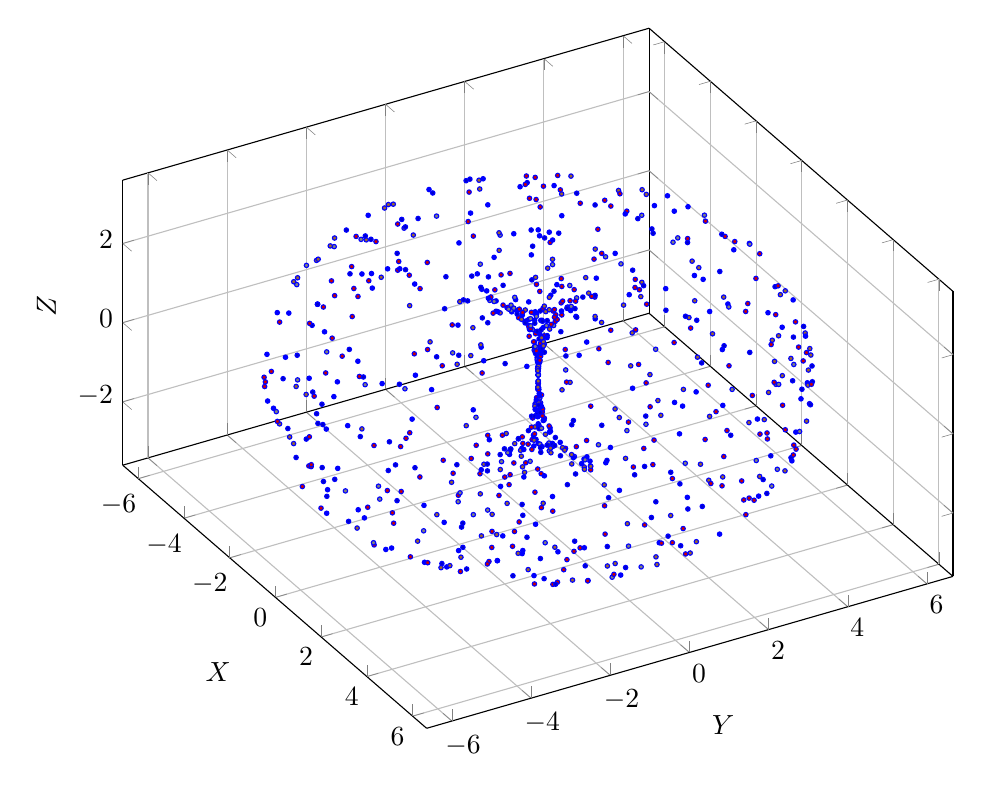
\begin{tikzpicture}
          \begin{axis}[
                view={60}{30},
                width=\textwidth, 
                axis equal,
                grid=major,
                xlabel={$X$},
                ylabel={$Y$},
                zlabel={$Z$},
        %        title={Random Points Inside a Horn Torus},
                samples=50,
                domain=0:360,
                y domain=0:360
            ]
            
            % Define parameters for a horn torus
            \pgfmathsetmacro{\R}{3}  % Major radius, set equal to minor radius
            \pgfmathsetmacro{\r}{3}  % Minor radius, set equal to major radius
            \pgfmathsetmacro{\thickness}{0.7} % Thickness to control the spread within the torus tube
        
            % Generate random points inside the horn torus
            \foreach \i in {1,...,888} {
                \pgfmathsetmacro{\theta}{random(0, 360)}
                \pgfmathsetmacro{\phi}{random(0, 360)}
                \pgfmathsetmacro{\radialDist}{\r + random(-\thickness, \thickness)}
                \pgfmathsetmacro{\x}{(\R + \radialDist * cos(\phi)) * cos(\theta)}
                \pgfmathsetmacro{\y}{(\R + \radialDist * cos(\phi)) * sin(\theta)}
                \pgfmathsetmacro{\z}{\radialDist * sin(\phi)}
        
                \addplot3+[only marks, mark=*, mark size=0.8pt, color=blue] coordinates {(\x, \y, \z)};
            }
            \end{axis}
        \end{tikzpicture}
    \caption[Horn Torus point cloud]{\textbf{Horn Torus point cloud.} Coded in to render in LaTeX with the help of ChatGPT $4$o.}
    \label{Wolfram Horn Torus}
\end{figure}
\clearpage



\section{The Data Visualisation Catalogue by Severino Ribecca}

\begin{figure}[h!]
    \centering
    \includegraphics[height=0.8\textheight]{figures/A.2.png}
    \caption[The Data Visualisation Catalogue]{\textbf{The Data Visualisation Catalogue.} 
\citep{ribecca_data_2017}. Used with Ribecca's permission.}
    \label{fig:A.2}
\end{figure}
\index[people]{Ribecca, Severino}
\clearpage

\section{Semantic Field \textit{S}}
\label{Appendix Semantic Field S}

In this section, I list the 310 terms of Semantic Field \textit{S}, as discussed in Chapter 5. To arrive at this list, I uploaded my thesis as a PDF to ChatGPT $4$o and parsed its keywords with the following prompt sequence: 
\begin{enumerate}
    \item[\textbf{1}] ``Categorize and list the key words in this document."
    \item[\textbf{2}] ``Write these as a list separated by commas, ranked by their relevance in the text"
\end{enumerate}

\rule{\linewidth}{0.4pt}


\begin{multicols}{4}
\begin{enumerate}[label=\arabic*.]
\item A Dish with One Spoon
\item abduction
\item Abundant Intelligences project
\item academic cross-pollination
\item academic knowledge management (AKM)
\item accessibility
\item Artificial General Intelligence (AGI)
\item AI energy consumption
\item algorithm
\item analogy
\item anti-oppression
\item Artificial Intelligence (AI)
\item axiological paradigms
\item biocultural memory
\item biodynamic agriculture
\item Blender
\item blind spots
\item Boundary Critique
\item capitalist extractivist economy
\item ChatGPT
\item Circle Semantic Shape
\item classification of natural forms
\item climate crisis
\item climate crisis mitigation
\item climate hyperobject
\item climate resilience
\item Carbon dioxide (CO2)
\item collaborative co-creation
\item collaborative Knowledge Production
\item colligative theory formation
\item complexity management
\item composition
\item Computational Analysis of Texts and Graphs (CATG)
\item Computational Graphesis
\item Computational Semiosis
\item conceptual gateways
\item Conceptual Graphs
\item Conceptual Networks
\item Cone Semantic Form
\item Cones of Plausibility
\item consilience
\item consilience across disciplines
\item Consilience in Knowledge Activation (CKA)
\item Consilience of Inductions
\item consolation
\item constellationary fields
\item conversational model
\item Creation-as-Research
\item Creative Presentations of Research
\item criminal justice system
\item Critical Systems Thinking (CST)
\item cybernetic mycelium
\item cybernetic rhizome
\item Cylinder Semantic Form
\item data activation
\item data hierarchy
\item data hierarchy visualization
\item data ontology modeling
\item data-information-knowledge-wisdom hierarchy (DIKW)
\item data-to-knowledge transformation
\item database of databases
\item decentralized knowledge structure
\item decomposition
\item deduction
\item degree-difference
\item Design for Health (DH)
\item Design for Sustainability Transitions (DfST)
\item Design with a Capital D
\item desolation
\item diagrammatic reasoning
\item Digital Humanities
\item dimensional addition
\item dimensionality
\item disciplinary interchange
\item discourse fields
\item domain models
\item double cone in optics
\item Double-Cone Semantic Form
\item double-diamond shape
\item eco-justice
\item ecoanthroposymbiosis
\item ecojustice
\item ecological cost of AI
\item ecologically informed AI strategy
\item Embedding Projector
\item energy resources
\item Entity-Relationship (ER) diagrams
\item environmental crisis
\item environmental degradation
\item environmental sustainability
\item epistemological diversity
\item Epistemology
\item Equity-Centered Community Design
\item Equity-Centered Community Design (ECCD)
\item ethnobotany
\item ethnoecology
\item Euclidean
\item evidence synthesis
\item filtration
\item formation and growth in morphology
\item funnel plot
\item futures cone
\item general consilience (GC)
\item Generous AI
\item geometric compositions
\item Gestalt psychology
\item gigamapping
\item glass box AI
\item Global Assortativity
\item Global Topological Synchronization (GTS)
\item GPT-3
\item GPT-4
\item graph embeddings
\item graph isomorphology
\item graph LLMs
\item graph morphology
\item graph of concepts
\item graph-based ontology models
\item graphesis
\item graphical user interface (GUI)
\item graphically structured knowledge
\item graphlet interface
\item graphlets
\item hierophanic
\item HITL (Human-in-the-Loop)
\item HITL CATG KA
\item Horn of Futures
\item Horn Torus Semantic Form
\item Human Analysis of Text and Graphs (HATG)
\item humanistic interface design
\item hyper-specialization
\item hyperlinked bibliometric graphing
\item hyperobject
\item incipit
\item Inclusive Design (ID)
\item induction
\item information design
\item information overload
\item information visualization
\item information visuospatialization
\item InfraNodus
\item interbeing
\item interdisciplinarity
\item interdisciplinary consilience
\item interdisciplinary Knowledge co-Production
\item interdisciplinary Knowledge Production
\item interdisciplinary synthesis
\item interdisciplinary topic mapping
\item Intergovernmental Panel on Climate Change (IPCC)
\item interpretable AI
\item isomorphic interbeing
\item isomorphogenesis
\item isomorphology
\item knowledge abstraction and synthesis
\item Knowledge Activation (KA)
\item knowledge design studio laboratory
\item knowledge engineering
\item knowledge graphs
\item Knowledge Management (KM)
\item Knowledge Production (KP)
\item Knowledge Production for Sustainability Transitions (KPST)
\item Knowledge Production through composition
\item Knowledge Production through visuospatial Semantic Form composition
\item Knowledge Pyramid
\item Knowledge Surfacing (KSu)
\item Knowledge Surfacing, Synthesis, Translation, and Creation(KSSTP)
\item Knowledge Synthesis (KSy)
\item Knowledge Translation (KT)
\item knowledge work platforms
\item KP quantification
\item Large Language Model (LLM)
\item logoi
\item logos of form
\item Logseq
\item Loop-line
\item Low-dimensional topology
\item ludic quality
\item major diameter
\item major radius
\item manual node placement
\item Markdown language
\item material infrastructure
\item Meru Chakra
\item meta-analysis
\item meta-language
\item meta-Systematic Combining (MSC)
\item metaphysics
\item methodological framework
\item methodological pluralism
\item middle ontology
\item minor diameter
\item minor radius
\item Mistral 7B
\item MNIST handwritten digits database
\item monocrops
\item morphology
\item moving spatial network graphs
\item multi-dimensional network graphs
\item multi-mathematical approach
\item multi-scale topological data features
\item natural resources
\item network graph
\item network graph composition
\item network graphlet
\item network subgraphs
\item networked data visualization
\item node grouping
\item Obsidian
\item Ontological Semantic Network Summaries (OSNS)
\item ontology
\item opaque AI
\item oppressive terminology
\item Oslo School of Systemic Design
\item outer diameter
\item outer radius
\item particle accelerator of ideas
\item Perceptual Artifacts Lab (PAL)
\item permaculture
\item Persistence Homology (PH)
\item Personal Knowledge Management (PKM)
\item perspective in art
\item plant-human co-evolution
\item point cloud
\item point plot heatmap
\item power relations
\item qualitative methods
\item Query Graphs
\item Query Isomorphs
\item rectangular coordinate system
\item Research-Creation
\item Research-for-Creation
\item Research-from-Creation
\item researcher grouping
\item rewilding
\item Ring Torus Semantic Form
\item Roam Research
\item Semantic Field S
\item Semantic Forms
\item semantic network mapping
\item Semantic Shapes
\item Semantic Topological Semiotics
\item simplicial complex
\item Small Language Models
\item social inequality
\item social justice
\item Social Sciences and Humanities Research Council
\item spatial and temporal modeling
\item spatial composition
\item spatial network graphs
\item spatial semiotic representation
\item spatial topic model network graphs
\item Sphere Semantic Form
\item Sri Yantra
\item stakeholder
\item Sustainability Transitions Knowledge Activation (STKA)
\item studio laboratory of knowledge design
\item surfaces of revolution
\item sustainability solutions frameworks
\item Sustainability Transitions (ST)
\item symbol composition
\item Symbol-setting
\item symbolic representation
\item syntopical consilience
\item Syntopical Consilience Abduction (SCA)
\item syntopical reading
\item Syntopicon
\item Systematic Combining (SC)
\item Systemic Design
\item Systemic Design Association (SDA)
\item Systems Oriented Design (SOD)
\item Systems Theory
\item Systems Thinking
\item Topological Capta Analysis (TCA)
\item TCA Researcher Grouping
\item TCA Workspace
\item tensors
\item Terroir of Text and Graphs (TTG)
\item text graphs
\item thought forms
\item thought signs
\item three-dimensional forms
\item three-dimensional information visualization
\item three-dimensional topic models
\item topic model network graphs
\item Topic Models
\item Topological Data Analysis (TDA)
\item Topological Capta Analysis (TCA)
\item topological semiotics
\item Topology
\item toroidal manifold
\item torus
\item transdisciplinary KA (Knowledge Activation)
\item Tree of Porphyry
\item UN Sustainable Development Goals (SDGs)
\item University
\item upper ontology
\item vector embeddings
\item vector search
\item Vedic visuospatial culture
\item visual argument
\item visual epistemology
\item visual reasoning
\item visuospatial epistemology
\item visuospatial forms of knowledge production
\item visuospatial knowledge activation interface
\item visuospatial reasoning
\item weighting
\item wicked problem
\item Zettelkasten
\item Zone of Semantic Stasis
\end{enumerate}
\end{multicols}
\clearpage

\section{Adler’s 102 \textit{Great Ideas}}
The following terms are listed alphabetically as per The \textit{Great Ideas: a Syntopicon of Great Books of the Western World} (1952), derived from the texts in \textit{Great Books of the Western World} (1952).
\begin{multicols}{4} % Use 2 or 3 columns, whichever fits well
\begin{enumerate}[label=\arabic*.]
    \item Angel
    \item Animal
    \item Aristocracy
    \item Art
    \item Astronomy and Cosmology
    \item Beauty
    \item Being
    \item Cause
    \item Chance
    \item Change
    \item Citizen
    \item Constitution
    \item Courage
    \item Custom and Convention
    \item Definition
    \item Democracy
    \item Desire
    \item Dialectic
    \item Duty
    \item Education
    \item Element
    \item Emotion
    \item Eternity
    \item Evolution
    \item Experience
    \item Family
    \item Fate
    \item Form
    \item God
    \item Good and Evil
    \item Government
    \item Habit
    \item Happiness
    \item History
    \item Honor
    \item Hypothesis
    \item Idea
    \item Immortality
    \item Induction
    \item Infinity
    \item Judgement
    \item Justice
    \item Knowledge
    \item Labor
    \item Language
    \item Law
    \item Liberty
    \item Life and Death
    \item Logic
    \item Love
    \item Man
    \item Mathematics
    \item Matter
    \item Mechanics
    \item Medicine
    \item Memory and Imagination
    \item Metaphysics
    \item Mind
    \item Monarch
    \item Nature
    \item Necessity and Contingency
    \item Oligarchy
    \item One and Many
    \item Opinion
    \item Opposition
    \item Philosophy
    \item Physics
    \item Pleasure and Pain
    \item Poetry
    \item Principle
    \item Progress
    \item Prophecy
    \item Prudence
    \item Punishment
    \item Quality
    \item Quantity
    \item Reasoning
    \item Relation
    \item Religion
    \item Revolution
    \item Rhetoric
    \item Same and Other
    \item Science
    \item Sense
    \item Sign and Symbol
    \item Sin
    \item Slavery
    \item Soul
    \item Space
    \item State
    \item Temperance
    \item Theology
    \item Time
    \item Truth
    \item Tyranny and Despotism
    \item Universal and Particular
    \item Virtue and Vice
    \item War and Peace
    \item Wealth
    \item Will
    \item Wisdom
    \item World
\end{enumerate}
\end{multicols} % Use 2 or 3 columns, whichever fits well
\clearpage


\section{Authors included in \textit{Great Books of the Western World} (1952)}
The \textit{Great Books of the Western World} (1952) includes works by the following authors:
\begin{multicols}{4}
\RaggedRight Homer\\
Aeschylus\\
Sophocles\\
Euripides\\
Aristophanes\\
Herodotus\\
Thucydides\\
Plato\\
Aristotle\\
Hippocrates\\
Galen\\
Euclid\\
Archimedes\\
Apollonius\\
Nichomachus\\
Lucretius\\
Epictetus\\
Marcus Aurelius\\
Virgil\\
Plutarch\\
Tacitus\\
Ptolemy\\
Copernicus\\
Kepler\\
Plotinus\\
Augustine\\
Thomas Aquinas\\
Dante\\
Chaucer\\
Machiavelli\\
Hobbes\\
Rabelais\\
Montaigne\\
Shakespeare\\
Gilbert\\
Galileo\\
Harvey\\
Cervantes\\
Francis Bacon\\
Descartes\\
Spinoza\\
Milton\\
Pascal\\
Newton\\
Huygens\\
Locke\\
Berkeley\\
Hume\\
Swift\\
Sterne\\
Fielding\\
Montesquieu\\
Rousseau\\
Adam Smith\\
Gibbon\\
Kant\\
J. S. Mill\\
Boswell\\
Lavoisier\\
Fourier\\
Faraday\\
Hegel\\
Goethe\\
Melville\\
Darwin\\
Marx\\
Engels\\
Tolstoy\\
Dostoyevsky\\
William James\\
Freud
\end{multicols}
\clearpage





\section{Categorizing the subjects of this thesis}
\raggedcolumns
\begin{multicols}{2}

\noindent\hangindent=1.5em \textbf{Computer Science} \\
Artificial Intelligence (AI) \\
Machine Learning \\
Natural Language Processing (NLP) \\
Computational Linguistics \\
Data Science \\
Human-Computer Interaction (HCI) \\
Information Retrieval \\
Knowledge Representation and Reasoning \\
Topological Data Analysis (TDA) \\
Graph Theory \\
\vspace{4mm}

\noindent\hangindent=1.5em \textbf{Mathematics} \\
Topology \\
Geometry \\
Computational Topology \\
Mathematical Modeling \\
\vspace{4mm}

\noindent\hangindent=1.5em \textbf{Philosophy} \\
Philosophy of Information \\
Philosophy of Language \\
Epistemology \\
Semiotics \\
Philosophy of Science \\
Ontology \\
\vspace{4mm}

\noindent\hangindent=1.5em \textbf{Cognitive Sciences} \\
Cognitive Psychology \\
Cognitive Neuroscience \\
Visual Cognition \\
Embodied Cognition \\
\vspace{4mm}

\noindent\hangindent=1.5em \textbf{Information Science} \\
Knowledge Management \\
Personal Knowledge Management (PKM) \\
Information Visualization \\
Library and Information Science \\
Ontologies \\
Digital Libraries \\
\vspace{4mm}

\noindent\hangindent=1.5em \textbf{Design} \\
Systems Oriented Design (SOD) \\
Systemic Design \\
Information Design \\
Visual Communication Design \\
Human-Centered Design \\
\vspace{4mm}

\noindent\hangindent=1.5em \textbf{Digital Humanities} \\
Computational Humanities \\
Digital Scholarship \\
Humanistic Interface Design \\
\vspace{4mm}

\noindent\hangindent=1.5em \textbf{Interdisciplinary Studies} \\
Sustainability Transitions \\
Environmental Studies \\
Climate Science \\
Ecojustice \\
Indigenous Studies \\
Decolonizing Methodologies \\
\vspace{4mm}

\noindent\hangindent=1.5em \textbf{Linguistics} \\
\RaggedRight Computational Linguistics \\
Semantics \\
Pragmatics \\
Language and Thought \\
\vspace{4mm}

\noindent\hangindent=1.5em \textbf{Education} \\
Knowledge Activation \\
Collaborative Learning \\
\RaggedRight Interdisciplinary Education \\
Educational Technology \\
\vspace{4mm}

\noindent\hangindent=1.5em \textbf{Sociology} \\
Sociology of Knowledge \\
Science and Technology Studies (STS) \\
Cultural Studies \\
\vspace{4mm}

\noindent\hangindent=1.5em \textbf{Communication Studies} \\
Media Studies \\
Information Theory \\
Symbolic Communication \\
\vspace{4mm}

\noindent\hangindent=1.5em \textbf{Ethnography and Anthropology} \\
Ethnoecology \\
Ethnobotany \\
Cultural Anthropology \\
\vspace{4mm}

\noindent\hangindent=1.5em \textbf{Visual Studies} \\
Visual Epistemology \\
Visual Reasoning \\
Visual Semiotics \\
Graphical Representation \\
\end{multicols}

\clearpage






\section{Experts consulted}
I acknowledge with professional admiration the subject matter experts who provided formative feedback for this thesis. I list their names here in alphabetical order by surname:

\begin{itemize}[label={}]
    \item \textbf{Dr. Evan Timothy Barba}, Associate Professor at Georgetown University
    \item \textbf{Tega Brain}, artist and Associate Professor at New York University (NYU)
    \item \textbf{Antionette D. Carroll}, founder of the Institute of Equitable Design and Justice, and Creative Reaction Labs
    \item \textbf{John P. Comer}, founder of Architects Of Justice; National Organizing Director of The Redress Movement
    \item \textbf{Dr.Peter Coppin}, Director of the The Perceptual Artifacts Lab (PAL) and  Associate Professor of Design at OCAD University. 
    \item \textbf{Dr. Sara Diamond}, OCAD University Research Chair, Director of the Visual Analytics Lab, and Co-investigator of the OCAD U Abundant Intelligences A Dish with One Spoon – Towards “Generous AI” Invention and Collaboration project
    \item \textbf{Dr. Michael Doser}, senior research physicist at the European Council for Nuclear Research/Conseil Européen pour la Recherche Nucléaire (CERN)
    \item \textbf{Balazs Farago}, founder and CEO of Walters Cube.
    \item \textbf{Ekaterina Grgurić}, Digital Scholarship Librarian at the University of British Columbia (UBC)
    \item \textbf{Michael Groenendyk}, Digital Scholarship Librarian at Concordia University
    \item \textbf{Micki Kaufman}, historian and digital scholar at the City University of New York
    \item \textbf{Dr. Peter Jones}, founder of the Strategic Innovation Lab, co-founder of the Systemic Design Association, and Distinguished Professor in Systemic Design for the School of Architecture, Art and Design at the Tecnológico de Monterrey
    \item \textbf{Amanda Licastro}, Digital Scholarship Librarian at Swarthmore College
    \item \textbf{Dr. Blake Madill}, Associate Professor of Pure Mathematics at the University of Waterloo
    \item \textbf{Cheryl May}, Executive Editor for the Systemic Design Association, and PhD candidate at London South Bank University
    \item \textbf{Dr. Gavin Mendel-Gleason}, CTO of TerminusDB, and former research fellow at Trinity College Dublin in the School of Statistics and Computer Science
    \item \textbf{Ola Mazzuca}, exhibition operations at the Gallery at Mason Studio
    \item \textbf{Antonio Muñoz Gomez}, Digital Scholarship Librarian at the University of Waterloo
    \item \textbf{Dr. Lennart Nacke}, University Research Chair and Professor at the University of Waterloo, and Associate Director of the Stratford School of Interaction Design and Business, and Director of the HCI Games Group at the University of Waterloo's Games Institute
    \item \textbf{Rahul Nayak}, data scientist from the Indian Institute of Technology
    \item \textbf{Dr. Dmitry Paranyushkin}, founder of InfraNodus and senior researcher at Nodus Labs
    \item \textbf{Dr. Paul Pangaro}, President of the American Society for Cybernetics
    \item \textbf{Dr. Michael J. Prokopow}, cultural historian, curator, and professor at OCAD University
    \item \textbf{Santiago Ortiz}, director of Moebio Labs
    \item \textbf{Ryan J. A. Murphy}, PhD candidate at the University of Newfoundland and Co-Secretary of the Systemic Design Association
    \item \textbf{Dr. Birger Sevaldson}, professor at the Oslo School of Architecture and Design, and at the University of South-Eastern Norway
    \item \textbf{Peter Scott}, lecturer at OCAD University
    \item \textbf{Dr. Maria Aleksandrovna Simakova}, Foucault scholar from the University of Toronto
    \item \textbf{Kirsta Stapelfeldt}, Associate Librarian, Research and Digital Initiatives at the University of Toronto Scarborough Digital Scholarship Unit
    \item \textbf{Brian Sunter}, software engineer from the University of Florida
    \item \textbf{Serkan Özkaya}, conceptual artist
    \item \textbf{David Kwasny}, Data and Digital Literacy Librarian at the University of Toronto Scarborough Digital Scholarship Unit
    \item \textbf{Kyle Winters}, CEO of NEXT Canada
\end{itemize}

\clearpage






\section{Research presentations}

In this section, I list the presentations I delivered about my work during my thesis research: \\

\begin{enumerate}


    \item[{2024}] \textit{Systems Oriented Disruptions}, presented for the annual International Innovation Forum hosted by the Strategic Foresight and Innovation program in the OCAD University School of Graduate Studies
 
    \item[{2024}] \textit{Systems Oriented Disruptions}, presented for Creative Disruptions// re-imagining our futures the graduate thesis exhibition by the Digital Futures program in the OCAD University’s School of Graduate Studies

    \item[{2024}]  \textit{Body of Aesthetics}, a panel discussion moderated by curator Sara Dagovic and joined by artist Artemis Han, The Gallery at Mason Studio, Toronto

    \item[{2023}] \textit{Three-dimensional plotting of information categories using P5.js}, Perceptual Artifacts Lab in OCAD University, moderated by the PAL Director Dr. Peter Coppin  

    \item[{2023}] \textit{Song Within a Sacrifice Zone}, presented for \textit{Uses and Abuses of Power in Alternative Spiritualities}, the annual conference by the Program for the Evolution of Spirituality in the Harvard Divinity School
 
    \item[{2023}] \textit{The biopower of faith leaders who are also alternative medicine practitioners in alternative spiritual communities}, presented for \textit{Uses and Abuses of Power in Alternative Spiritualities}, the annual conference by the Program for the Evolution of Spirituality in the Harvard Divinity School
 
    \item[{2023}] \textit{Knowledge Translation vs the Climate Crisis} presented for the annual colloquium hosted by the Digital Futures in the OCAD University School of Graduate Studies
 
    \item[{2022}] \textit{Dissonance}, presented for the Too Big To Fail Exhibition organized by the Interdisciplinary Master’s of Art, Media and Design in the OCAD University School of Graduate Studies

    \item[{2022}] \textit{Data Tori}, presented for the annual Graduate Colloquium, moderated by Duchamp scholar Dr. Julian Haladyn, in the OCAD University School of Graduate Studies

    \item[{2022}] \textit{Medicinallity of Symbol}, presented for the annual research panel organized by the Interdisciplinary Master’s of Art, Media and Design, in the OCAD University School of Graduate Studies, moderated by Graduate Program Director Jay Irizawa
    
\end{enumerate}
\clearpage




\section{Art exhibitions}

In this section, I list the art exhibitions in which I showcased my work during my thesis research: \\

\begin{enumerate}
    \item[{2024}] \textit{GradEx 109}, OCAD University

    \item[{2024}] \textit{Creative Disruptions// re-imagining our futures}, Digital Futures graduate thesis exhibition, OCAD University, Waterfront Campus. 
 
    \item[{2024}] \textit{Body of Aesthetics, curated by Sara Dagovic}, The Gallery at Mason Studio, Toronto

    \item[{2023}] \textit{Digital Futures Open Show}, OCAD University, School of Graduate Studies

    \item[{2023}] \textit{Song Within a Sacrifice Zone}, Harvard Divinity School, Swartz Hall
 
    \item[{2023}] \textit{Resilience and Connection: artistic explorations of mental health}, L.R. Wilson Building, McMaster University 
 
    \item[{2023}] \textit{Too Big to Fail}, Open Space Gallery, OCADU
 
    \item[{2022}] \textit{The Incomplete}, The Great Hall Gallery, OCADU
\end{enumerate}
\clearpage





\section{Resources and tools tested and used during thesis}
\label{Appendix Resources and Tools}
\begin{multicols}{2}

\noindent\hangindent=1.5em \textbf{Hardware} \\
Macbook Pro, 16-inch, 2021, Apple M1 Max, 32 GB RAM

\vspace{4mm}

\noindent\hangindent=1.5em \textbf{Source Management} \\
Zotero \\
\RaggedRight \hangindent=1.5em Zotero Better BibTex extension v 6.7.202 by Emiliano Heyns (to generate citation keys) \\
Zotero Connector Chrome extension \\

\vspace{4mm}

\noindent\hangindent=1.5em \textbf{Personal Knowledge Management (PKM)} \\
Obsidian \\
Logseq \\
Logseq PDF reader \\
Readwise Official Plugin v1.4.9 \\
Roam Research \\
\vspace{4mm}
\noindent\hangindent=1.5em \textbf{Three-Dimensional Forms} \\
Blender, node programming \\

\vspace{4mm}

\noindent\hangindent=1.5em \textbf{Document Drafting} \\
\RaggedRight \hangindent=1.5em Overleaf, Online LaTeX editor \\
\RaggedRight \hangindent=1.5em Dissertate, LaTeX dissertation template by Jordan Suchow \\
\RaggedRight \hangindent=1.5em Pandoc for populating Better BibTeX citation keys into in-sentence citation and list of references \\
Google Docs \\
Google Chrome extension DocsAfter Dark \\
Microsoft Word \\

\vspace{4mm}

\noindent\hangindent=1.5em \textbf{Document Reading} \\
Zotero PDF reader \\
ProQuest Ebook Central \\
The Internet Archive \\
Logseq PDF reader \\
Readwise \\
Readwise Reader \\
\RaggedRight \hangindent=1.5em Readwise Chrome extension (synced to Logseq and Obsidian) \\
Apple Photos Optical Character Recognition \\
Adobe Acrobat \\
Adobe Digital Editions \\

\vspace{4mm}

\noindent\hangindent=1.5em \textbf{Infinite Canvas Text Analysis Tools} \\
Miro \\
Scapple \\

\vspace{4mm}

\noindent\hangindent=1.5em \textbf{Text Graphing Tools} \\
InfraNodus \\
\RaggedRight \hangindent=1.5em InfraNodus Chrome extension for its 3D knowledge graph \\
MIT’s SIMILE Timeline widget, run on Zotero \\
Obsidian Canvas, core plugin \\ 
Obsidian Outline, core plugin \\
Obsidian Graph View, core plugin \\
\RaggedRight \hangindent=1.5em Obsidian 3D Graph v1.0.5, community plugin by Alexander Weichart \\
Python 3.8.12 \\
PiVis* \\
Pandas Dataframes* \\
NetworkX* \\
Voyant Tools \\
* Python libraries \\

\vspace{4mm}


\noindent\hangindent=1.5em \textbf{LLMs} \\
Mistral 7B Open Orca* \\
Zephyr* \\
Grammarly AI Writing Assistant \\
Claude 3.5 Sonnet \\
Google Gemini Advanced 1.5 Pro\\
Chat GPT 3.5 \\
Chat GPT 4 \\
Chat GPT 4 Turbo \\
Chat GPT $4$o \\
Chat GPT 4-mini \\
Chat GPT o1-preview \\
Chat GPT o1 \\
Chat GPT o1-mini \\
* set up using Ollama \\

\vspace{4mm}


\noindent\hangindent=1.5em \textbf{Image Management} \\
Apple Photos \\
Affinity \\
Affinity Designer \\
Affinity Publisher \\
Pinterest \\
QuickTime Player \\

\vspace{4mm}

\noindent\hangindent=1.5em \textbf{Audio and Video Production} \\
\RaggedRight Final Cut Pro \\ 
\RaggedRight Logic Pro \\

\vspace{4mm}

\noindent\hangindent=1.5em \textbf{Typefaces in Figures} \\
iA Writer Quattro S \\
Helvetica Neue \\
Arial Black \\
Avenir Next Condensed \\

\vspace{4mm}

\noindent\hangindent=1.5em \textbf{Typefaces in Document} \\
Lato - used for text captions \\
Noto Mono - used for code \\
EB Garramond - used for all other text \\

\end{multicols}

\clearpage

%\chapter*{Indices}
%\addcontentsline{toc}{chapter}{Indices}
%\label{Index}




%Testing <<<


\singlespacing
% the back matter
\clearpage
\sloppy % Added 2024 Nov 1
\bibliographystyle{elsarticle-harv}
\bibliography{references}
\addcontentsline{toc}{chapter}{References}
%\printbibliography
%\include{endmatter/colophon}
\printindex[people]
\addcontentsline{toc}{chapter}{Author index}
\clearpage
\printindex[terms]
\addcontentsline{toc}{chapter}{Subject index}
\clearpage

\chapter*{Invitation}
\addcontentsline{toc}{chapter}{Invitation}
\label{Invitation}
\noindent
    \setstretch{1.5} % Adjust line spacing
%    \vspace*{\fill}
\begin{quote}
    To recall a humorous example from the origins of computational text methods, Tim Berners-Lee’s Information Management (1989) was received by his supervisor Mike Sendall as “Vague, but exciting…” \citep{cern_tim_2008}. In this thesis I advocate for giving novel ideas a chance, even if they are not fully formed, including my own. If you are a topologist or computer scientist inclined to lean forward past vagueness into excitement, I heartily welcome your collaboration. To reach me, email mateocs[at]ocadu[dot]ca, or visit studiomto[dot]com.
\end{quote}
    \vspace*{\fill} % Center content vertically
    \newpage
\chapter*{\centering About the author}
\addcontentsline{toc}{chapter}{About the author}
\label{About the author}
\noindent
    \setstretch{2} % Adjust line spacing
%    \vspace*{\fill}
\begin{quote}
    Orus Mateo Castaño-Suárez contributes to the Harvard Divinity School (HDS) Program for the Evolution of Spirituality (PES), the Abundant Intelligences (AbInt) Indigenous AI project, the American Society for Cybernetics (ASC), and the Systemic Design Association (SDA). In Toronto, Castaño-Suárez is a contributor to the OCAD University Global Centre for Climate Action (GCCA), the Visual Analytics Lab (VAL), the A Dish with One Spoon—Towards “Generous AI” Invention and Collaboration project, and the Strategic Innovation Lab (sLab). Castaño-Suárez's research is supported by the Ontario Graduate Scholarship and others.
\end{quote}
    \vspace*{\fill} % Center content vertically
    \newpage
\end{document}




%Code Archive:

% Not working
%decomission date: 2025 Jan 11
%>>>
%\begin{appendices} 
%    \renewcommand{\thechapter}{\Alph{chapter}} % Use letters for appendices
%    \chapter[Appendix]{Appendix}
\label{Appendix}
\section{Thesis website}
The ongoing developments of this thesis research and a gallery of moving Semantic Form models are available on the following website: 

\url{https://studiomto.square.site/thesis-what-may-be-known-2024}

\section{LaTeX manuscript repository}
The following web page provides access to the LaTeX code used to compile this thesis, including all figures and formatting details:

\url{https://github.com/orusmateo/Orus-MCS-Thesis}

\section{Moving and interactive models}
The following web page provides access to the moving and interactive models developed for my thesis. 

\url{https://studiomto.square.site/moving-semforms}

\section{Semantic Forms surface and volume equations }
\label{Semantic Forms equations}
\begin{table}[h]
    \centering
    \begin{tabular}{|l|l|l|}
\hline
 & \textit{Volume (V)} & \textit{Surface (S)} \\[10pt]
 \hline
cone &  $\pi r^2 \frac{h}{3}$ & $\pi r \sqrt{r^2+h^2}$  \\[10pt] \hline
 cylinder & $\pi r^2 h$ & $2 \pi r h$ \\[10pt]
  \hline
sphere & $\frac{4}{3} \pi  R^3$ & $4 \pi r^2$ \\[10pt] \hline
horn torus & $2 \pi^2 a^3$ & $4 \pi^2 a^2$ \\[10pt] \hline
ring torus & $\frac{1}{4} \pi^2(R+r)(R-r) a^*$ & $\pi^2 (R+r)(R-r)$ \\[10pt]
\hline
\multicolumn{3}{l}

    \end{tabular}
    %\caption{Caption}
\end{table}

\begin{quote}
    \centering *Pappus’s centroid theorem \citep{weisstein_torus_nodate}.
\end{quote}

\index[people]{Pappus}
\clearpage

\section{Application of Sarajlić et al. configurations to three-dimensional graphlets}
As part of my style guide for Query Isomorphs analysis I propose that the Sarajlić et al. graphlet configurations \citep[p. 3]{sarajlic_graphlet-based_2016} can be used for graph input and graph analysis.

\begin{figure}[h!]
    \centering
    \includegraphics[width=0.8\textwidth]{figures/5.6.png}
    \caption[Example Query Isomorph in two dimensions and three dimensions assembled from directed graphlets]{\textbf{Example Query Isomorph in two dimensions and three dimensions assembled from directed graphlets.} \\
(a) From Sarajlić et al. 2016’s point b, “Illustration of how directed graphlets assemble together to form complex networks”, from “Figure 1. Illustration of directed graphlets” \citep[p. 3]{sarajlic_graphlet-based_2016}. In keeping with Sarajlić et al., the whole network can be created by adding graphlet G4, G1, and G3, meaning that in the process a new graphlet, G2, was created. The colours red, green, blue, and black are sourced from \citep[p. 3]{sarajlic_graphlet-based_2016}. (b) Spatial arrangement adds semantic value of verticality to communicate hierarchy of the blue node.  Red nodes are querying for nodes in both higher and lateral hierarchy. (c) Other arrangements can easily facilitate different relationships in the Query Isomorph. (b) and (c) The colours red, green, blue, are sourced from \citep[p. 3]{sarajlic_graphlet-based_2016} here also, but white is used instead of black for contrast. Black nodes in this example are all placed in a lateral level of hierarchy. In a functional Query Isomorph platform, nodes could also be placed higher or lower to each other. Furthermore, the angles and directions of these graphlets are presented for simplicity of the variety they can have, but does not represent the diversity of angle and form that graphlets can be configured in as Query Isomorphs. 
}
    \label{f5.6}
\end{figure}
\clearpage


\section{The Semantic Forms located in Bertin’s taxonomy of network graphs}
\begin{figure}[h!]
    \centering
    \includegraphics[width=0.9\textwidth]{figures/A.3.png}
    \caption[Groups of imposition and types of imposition]{\textbf{Groups of imposition and types of imposition} \citep[p. 52]{bertin_semiology_2011}.
From \textit{Semiology of Graphics: Diagrams, Networks, Maps} by Jacques Bertin, translated by William J. Berg. Reprinted by permission of the University of Wisconsin Press. © 1983 by the Board of Regents of the University of Wisconsin System. All rights reserved.}
    \label{fig:A3}
\end{figure}
%\clearpage
\begin{figure}[h!]
    \centering
    \includegraphics[width=\textwidth]{figures/A.4.png}
    \caption[Groups of imposition and types of imposition as categories for my Semantic Shapes, Semantic Forms, and three-dimensional gigamaps]{\textbf{Groups of imposition and types of imposition as categories for my Semantic Shapes, Semantic Forms, and three-dimensional gigamaps}. My work is overlaid onto Bertin’s categorization of network diagrams \citep[p. 52]{bertin_semiology_2011} from \textit{Semiology of Graphics: Diagrams, Networks, Maps} by Jacques Bertin, translated by William J. Berg. Reprinted by permission of the University of Wisconsin Press. © 1983 by the Board of Regents of the University of Wisconsin System. All rights reserved.}
    \label{fig:A4}
\end{figure}
%\clearpage
\begin{figure}[h!]
    \centering
    \includegraphics[height=0.8\textheight]{figures/A.5.png}
    \caption[Implantation and imposition of network diagrams]{\textbf{Implantation and imposition of network diagrams} \citep[p. 270]{bertin_semiology_2011} \\
From \textit{Semiology of Graphics: Diagrams, Networks, Maps} by Jacques Bertin, translated by William J. Berg. Reprinted by permission of the University of Wisconsin Press. © 1983 by the Board of Regents of the University of Wisconsin System. All rights reserved.}
    \label{fig:A5}
\end{figure}
\begin{figure}[h!]
    \centering
    \includegraphics[width=\textwidth]{figures/A.6.png}
    \caption[Implantation and imposition of network diagrams as categories for my Semantic Shapes, Semantic Forms, and three-dimensional gigamaps]{\textbf{Implantation and imposition of network diagrams as categories for my Semantic Shapes, Semantic Forms, and three-dimensional gigamaps.} \citep[p. 270]{bertin_semiology_2011} 
My work is overlaid onto Bertin’s categorization of network diagrams \citep[p. 270]{bertin_semiology_2011} from \textit{Semiology of Graphics: Diagrams, Networks, Maps} by Jacques Bertin, translated by William J. Berg. Reprinted by permission of the University of Wisconsin Press. © 1983 by the Board of Regents of the University of Wisconsin System. All rights reserved.
}
    \label{fig:A6}
\end{figure}
\clearpage


\section{Graphical abstract}
\begin{figure}[h!]
    \centering
    \includegraphics[width=\textwidth]{figures/AF1.pdf}
    \caption[Graphical abstract]{\textbf{Graphical abstract}}
    \label{fig:graphical_abstract}
 \clearpage
\end{figure}
\clearpage


\section{Horn of futures}
\FloatBarrier
\begin{figure}[h!]
    \centering
    \includegraphics[width=\textwidth]{figures/5.29.png}
    \caption[Horn of Futures]{\textbf{Horn of Futures.} This figure depicts the 2D dimensional reduction of the bottom view of a modified 3D Cone of Plausibility \citep[p. 14]{taylor_creating_1990} \citep[p. 73]{bezold_overview_1993}. This Cone Semantic Form is curved into a spiral similar to \autoref{fig:18} “Diagram of a design process with iterations” \citep[p. 343]{sevaldson_designing_2022} \citep{sevaldson_designing_2022-1}. The 3D version of this form twists like a ram’s horn, and this thesis involves the study of the horn torus, hence the name \textit{Horn of Futures}}
    \label{f5.29}
\end{figure}
\FloatBarrier
\clearpage







\section{Horn Torus point cloud}
\begin{figure}[h!]
    \centering
        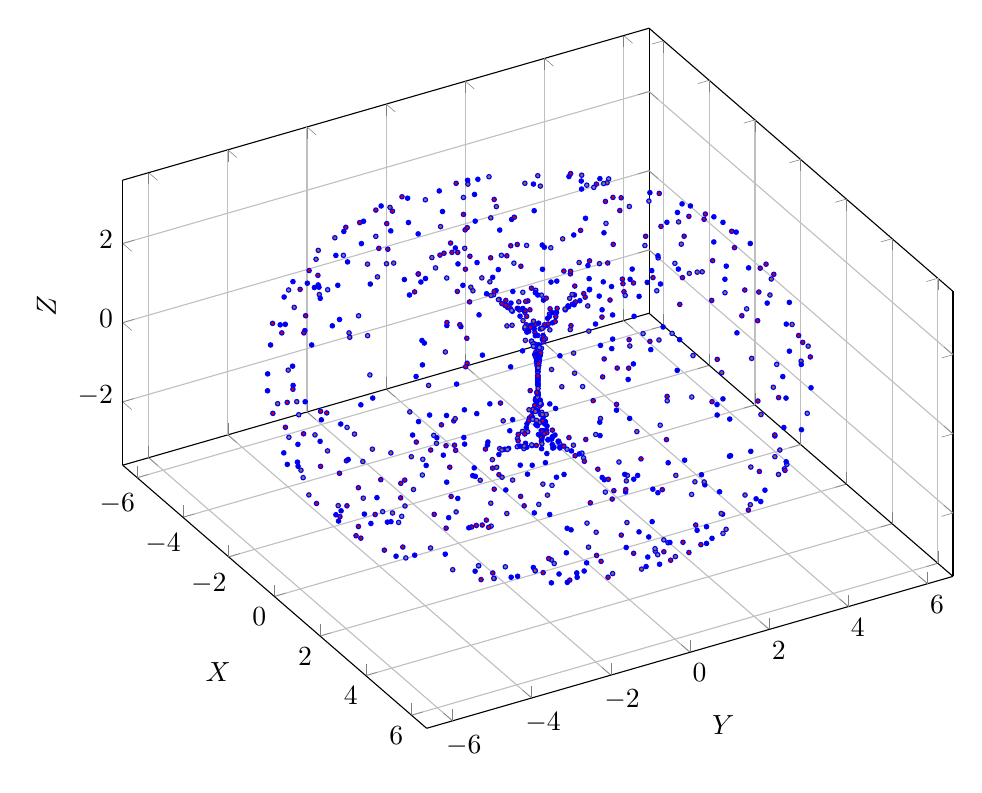
\begin{tikzpicture}
          \begin{axis}[
                view={60}{30},
                width=\textwidth, 
                axis equal,
                grid=major,
                xlabel={$X$},
                ylabel={$Y$},
                zlabel={$Z$},
        %        title={Random Points Inside a Horn Torus},
                samples=50,
                domain=0:360,
                y domain=0:360
            ]
            
            % Define parameters for a horn torus
            \pgfmathsetmacro{\R}{3}  % Major radius, set equal to minor radius
            \pgfmathsetmacro{\r}{3}  % Minor radius, set equal to major radius
            \pgfmathsetmacro{\thickness}{0.7} % Thickness to control the spread within the torus tube
        
            % Generate random points inside the horn torus
            \foreach \i in {1,...,888} {
                \pgfmathsetmacro{\theta}{random(0, 360)}
                \pgfmathsetmacro{\phi}{random(0, 360)}
                \pgfmathsetmacro{\radialDist}{\r + random(-\thickness, \thickness)}
                \pgfmathsetmacro{\x}{(\R + \radialDist * cos(\phi)) * cos(\theta)}
                \pgfmathsetmacro{\y}{(\R + \radialDist * cos(\phi)) * sin(\theta)}
                \pgfmathsetmacro{\z}{\radialDist * sin(\phi)}
        
                \addplot3+[only marks, mark=*, mark size=0.8pt, color=blue] coordinates {(\x, \y, \z)};
            }
            \end{axis}
        \end{tikzpicture}
    \caption[Horn Torus point cloud]{\textbf{Horn Torus point cloud.} Created for LaTeX with the help of ChatGPT 4o.}
    \label{Wolfram Horn Torus}
\end{figure}
\clearpage



\section{The Data Visualisation Catalogue by Severino Ribecca}

\begin{figure}[h!]
    \centering
    \includegraphics[height=0.8\textheight]{figures/A.2.png}
    \caption[The Data Visualisation Catalogue]{\textbf{The Data Visualisation Catalogue.} 
\citep{ribecca_data_2017}. Used with permission.}
    \label{fig:A.2}
\end{figure}

\clearpage

\section{Semantic Field \textit{S}}

\begin{multicols}{4}
\begin{enumerate}[label=\arabic*.]
\item A Dish with One Spoon
\item abduction
\item Abundant Intelligences project
\item academic cross-pollination
\item academic knowledge management (AKM)
\item accessibility
\item Artificial General Intelligence (AGI)
\item AI energy consumption
\item algorithm
\item analogy
\item anti-oppression
\item Artificial Intelligence (AI)
\item axiological paradigms
\item biocultural memory
\item biodynamic agriculture
\item Blender
\item blind spots
\item Boundary Critique
\item capitalist extractivist economy
\item ChatGPT
\item Circle Semantic Shape
\item classification of natural forms
\item climate crisis
\item climate crisis mitigation
\item climate hyperobject
\item climate resilience
\item Carbon dioxide (CO2)
\item collaborative co-creation
\item collaborative Knowledge Production
\item colligative theory formation
\item complexity management
\item composition
\item Computational Analysis of Texts and Graphs (CATG)
\item computational graphesis
\item computational semiosis
\item conceptual gateways
\item Conceptual Graphs
\item Conceptual Networks
\item Cone Semantic Form
\item Cones of Plausibility
\item consilience
\item consilience across disciplines
\item Consilience in Knowledge Activation (CKA)
\item Consilience of Inductions
\item consolation
\item constellationary fields
\item conversational model
\item Creation-as-Research
\item Creative Presentations of Research
\item criminal justice system
\item Critical Systems Thinking (CST)
\item cybernetic mycelium
\item cybernetic rhizome
\item Cylinder Semantic Form
\item data activation
\item data hierarchy
\item data hierarchy visualization
\item data ontology modeling
\item data-information-knowledge-wisdom hierarchy (DIKW)
\item data-to-knowledge transformation
\item database of databases
\item decentralized knowledge structure
\item decomposition
\item deduction
\item degree-difference
\item Design for Health (DH)
\item Design for Sustainability Transitions (DfST)
\item Design with a Capital D
\item desolation
\item diagrammatic reasoning
\item Digital Humanities
\item dimensional addition
\item dimensionality
\item disciplinary interchange
\item discourse fields
\item domain models
\item double cone in optics
\item Double-Cone Semantic Form
\item double-diamond shape
\item eco-justice
\item ecoanthroposymbiosis
\item ecojustice
\item ecological cost of AI
\item ecologically informed AI strategy
\item Embedding Projector
\item energy resources
\item Entity-Relationship (ER) diagrams
\item environmental crisis
\item environmental degradation
\item environmental sustainability
\item epistemological diversity
\item Epistemology
\item Equity-Centered Community Design
\item Equity-Centered Community Design (ECCD)
\item ethnobotany
\item ethnoecology
\item Euclidean
\item evidence synthesis
\item filtration
\item formation and growth in morphology
\item funnel plot
\item futures cone
\item general consilience (GC)
\item Generous AI
\item geometric compositions
\item Gestalt psychology
\item gigamapping
\item glass box AI
\item Global Assortativity
\item Global Topological Synchronization (GTS)
\item GPT-3
\item GPT-4
\item graph embeddings
\item graph isomorphology
\item graph LLMs
\item graph morphology
\item graph of concepts
\item graph-based ontology models
\item graphesis
\item graphical user interface (GUI)
\item graphically structured knowledge
\item graphlet interface
\item graphlets
\item hierophanic
\item HITL (Human-in-the-Loop)
\item HITL CATG KA
\item Horn of Futures
\item Horn Torus Semantic Form
\item Human Analysis of Text and Graphs (HATG)
\item humanistic interface design
\item hyper-specialization
\item hyperlinked bibliometric graphing
\item hyperobject
\item incipit
\item Inclusive Design (ID)
\item induction
\item information design
\item information overload
\item information visualization
\item information visuospatialization
\item InfraNodus
\item interbeing
\item interdisciplinarity
\item interdisciplinary consilience
\item interdisciplinary Knowledge co-Production
\item interdisciplinary Knowledge Production
\item interdisciplinary synthesis
\item interdisciplinary topic mapping
\item Intergovernmental Panel on Climate Change (IPCC)
\item interpretable AI
\item isomorphic interbeing
\item isomorphogenesis
\item isomorphology
\item knowledge abstraction and synthesis
\item Knowledge Activation (KA)
\item knowledge design studio laboratory
\item knowledge engineering
\item knowledge graphs
\item Knowledge Management (KM)
\item Knowledge Production (KP)
\item Knowledge Production for Sustainability Transitions (KPST)
\item Knowledge Production through composition
\item Knowledge Production through visuospatial Knowledge Form composition
\item Knowledge Pyramid
\item Knowledge Surfacing (KS)
\item Knowledge Surfacing, Synthesis, Translation, and Creation(KSSTP)
\item Knowledge Synthesis (KS)
\item Knowledge Translation (KT)
\item knowledge work platforms
\item KP quantification
\item Large Language Model (LLM)
\item logoi
\item logos of form
\item Logseq
\item Loop-line
\item Low-dimensional topology
\item ludic quality
\item major diameter
\item major radius
\item manual node placement
\item Markdown language
\item material infrastructure
\item Meru Chakra
\item meta-analysis
\item meta-language
\item meta-Systematic Combining (MSC)
\item metaphysics
\item methodological framework
\item methodological pluralism
\item middle ontology
\item minor diameter
\item minor radius
\item Mistral 7B
\item MNIST handwritten digits database
\item monocrops
\item morphology
\item moving spatial network graphs
\item multi-dimensional network graphs
\item multi-mathematical approach
\item multi-scale topological data features
\item natural resources
\item network graph
\item network graph composition
\item network graphlet
\item network subgraphs
\item networked data visualization
\item node grouping
\item Obsidian
\item Ontological Semantic Network Summaries (OSNS)
\item ontology
\item opaque AI
\item oppressive terminology
\item Oslo School of Systemic Design
\item outer diameter
\item outer radius
\item particle accelerator of ideas
\item Perceptual Artifacts Lab (PAL)
\item permaculture
\item Persistence Homology (PH)
\item Personal Knowledge Management (PKM)
\item perspective in art
\item plant-human co-evolution
\item point cloud
\item point plot heatmap
\item power relations
\item qualitative methods
\item query graphs
\item Query Isomorphs
\item rectangular coordinate system
\item Research-Creation
\item Research-for-Creation
\item Research-from-Creation
\item researcher grouping
\item rewilding
\item Ring Torus Semantic Form
\item Roam Research
\item Semantic Field S
\item Semantic Forms
\item semantic network mapping
\item Semantic Shapes
\item Semantic Topological Semiotics
\item simplicial complex
\item Small Language Models
\item social inequality
\item social justice
\item Social Sciences and Humanities Research Council
\item spatial and temporal modeling
\item spatial composition
\item spatial network graphs
\item spatial semiotic representation
\item spatial topic model network graphs
\item Sphere Semantic Form
\item Sri Yantra
\item stakeholder
\item Sustainability Transitions Knowledge Activation (STKA)
\item studio laboratory of knowledge design
\item surfaces of revolution
\item sustainability solutions frameworks
\item Sustainability Transitions (ST)
\item symbol composition
\item Symbol-setting
\item symbolic representation
\item syntopical consilience
\item Syntopical Consilience Abduction (SCA)
\item syntopical reading
\item Syntopicon
\item Systematic Combining (SC)
\item Systemic Design
\item Systemic Design Association (SDA)
\item Systems Oriented Design (SOD)
\item Systems Theory
\item Systems Thinking
\item Topological Capta Analysis (TCA)
\item TCA Researcher Grouping
\item TCA Workspace
\item tensors
\item Terroir of Text and Graphs (TTG)
\item text graphs
\item thought forms
\item thought signs
\item three-dimensional forms
\item three-dimensional information visualization
\item three-dimensional topic models
\item topic model network graphs
\item Topic Models
\item Topological Data Analysis (TDA)
\item Topological Capta Analysis (TCA)
\item topological semiotics
\item Topology
\item toroidal manifold
\item torus
\item transdisciplinary KA (Knowledge Activation)
\item Tree of Porphyry
\item UN Sustainable Development Goals (SDGs)
\item University
\item upper ontology
\item vector embeddings
\item vector search
\item Vedic visuospatial culture
\item visual argument
\item visual epistemology
\item visual reasoning
\item visuospatial epistemology
\item visuospatial forms of knowledge production
\item visuospatial knowledge activation interface
\item visuospatial reasoning
\item weighting
\item wicked problem
\item Zettelkasten
\item Zone of Semantic Stasis
\end{enumerate}
\end{multicols}
\clearpage

\section{Adler’s 102 \textit{Great Ideas}}
The following terms are listed alphabetically as per The \textit{Great Ideas: a Syntopicon of Great Books of the Western World} (1952), derived from the texts in \textit{Great Books of the Western World} (1952).
\begin{multicols}{4} % Use 2 or 3 columns, whichever fits well
\begin{enumerate}[label=\arabic*.]
    \item Angel
    \item Animal
    \item Aristocracy
    \item Art
    \item Astronomy and Cosmology
    \item Beauty
    \item Being
    \item Cause
    \item Chance
    \item Change
    \item Citizen
    \item Constitution
    \item Courage
    \item Custom and Convention
    \item Definition
    \item Democracy
    \item Desire
    \item Dialectic
    \item Duty
    \item Education
    \item Element
    \item Emotion
    \item Eternity
    \item Evolution
    \item Experience
    \item Family
    \item Fate
    \item Form
    \item God
    \item Good and Evil
    \item Government
    \item Habit
    \item Happiness
    \item History
    \item Honor
    \item Hypothesis
    \item Idea
    \item Immortality
    \item Induction
    \item Infinity
    \item Judgement
    \item Justice
    \item Knowledge
    \item Labor
    \item Language
    \item Law
    \item Liberty
    \item Life and Death
    \item Logic
    \item Love
    \item Man
    \item Mathematics
    \item Matter
    \item Mechanics
    \item Medicine
    \item Memory and Imagination
    \item Metaphysics
    \item Mind
    \item Monarch
    \item Nature
    \item Necessity and Contingency
    \item Oligarchy
    \item One and Many
    \item Opinion
    \item Opposition
    \item Philosophy
    \item Physics
    \item Pleasure and Pain
    \item Poetry
    \item Principle
    \item Progress
    \item Prophecy
    \item Prudence
    \item Punishment
    \item Quality
    \item Quantity
    \item Reasoning
    \item Relation
    \item Religion
    \item Revolution
    \item Rhetoric
    \item Same and Other
    \item Science
    \item Sense
    \item Sign and Symbol
    \item Sin
    \item Slavery
    \item Soul
    \item Space
    \item State
    \item Temperance
    \item Theology
    \item Time
    \item Truth
    \item Tyranny and Despotism
    \item Universal and Particular
    \item Virtue and Vice
    \item War and Peace
    \item Wealth
    \item Will
    \item Wisdom
    \item World
\end{enumerate}
\end{multicols} % Use 2 or 3 columns, whichever fits well
\clearpage


\section{Authors included in \textit{Great Books of the Western World} (1952)}
The \textit{Great Books of the Western World} (1952) includes works by the following authors:
\begin{multicols}{4}
\RaggedRight Homer\\
Aeschylus\\
Sophocles\\
Euripides\\
Aristophanes\\
Herodotus\\
Thucydides\\
Plato\\
Aristotle\\
Hippocrates\\
Galen\\
Euclid\\
Archimedes\\
Apollonius\\
Nichomachus\\
Lucretius\\
Epictetus\\
Marcus Aurelius\\
Virgil\\
Plutarch\\
Tacitus\\
Ptolemy\\
Copernicus\\
Kepler\\
Plotinus\\
Augustine\\
Thomas Aquinas\\
Dante\\
Chaucer\\
Machiavelli\\
Hobbes\\
Rabelais\\
Montaigne\\
Shakespeare\\
Gilbert\\
Galileo\\
Harvey\\
Cervantes\\
Francis Bacon\\
Descartes\\
Spinoza\\
Milton\\
Pascal\\
Newton\\
Huygens\\
Locke\\
Berkeley\\
Hume\\
Swift\\
Sterne\\
Fielding\\
Montesquieu\\
Rousseau\\
Adam Smith\\
Gibbon\\
Kant\\
J. S. Mill\\
Boswell\\
Lavoisier\\
Fourier\\
Faraday\\
Hegel\\
Goethe\\
Melville\\
Darwin\\
Marx\\
Engels\\
Tolstoy\\
Dostoyevsky\\
William James\\
Freud
\end{multicols}
\clearpage





\section{Categorizing the subjects of this thesis}
\raggedcolumns
\begin{multicols}{2}

\noindent\hangindent=1.5em \textbf{Computer Science} \\
Artificial Intelligence (AI) \\
Machine Learning \\
Natural Language Processing (NLP) \\
Computational Linguistics \\
Data Science \\
Human-Computer Interaction (HCI) \\
Information Retrieval \\
Knowledge Representation and Reasoning \\
Topological Data Analysis (TDA) \\
Graph Theory \\
\vspace{4mm}

\noindent\hangindent=1.5em \textbf{Mathematics} \\
Topology \\
Geometry \\
Computational Topology \\
Mathematical Modeling \\
\vspace{4mm}

\noindent\hangindent=1.5em \textbf{Philosophy} \\
Philosophy of Information \\
Philosophy of Language \\
Epistemology \\
Semiotics \\
Philosophy of Science \\
Ontology \\
\vspace{4mm}

\noindent\hangindent=1.5em \textbf{Cognitive Sciences} \\
Cognitive Psychology \\
Cognitive Neuroscience \\
Visual Cognition \\
Embodied Cognition \\
\vspace{4mm}

\noindent\hangindent=1.5em \textbf{Information Science} \\
Knowledge Management \\
Personal Knowledge Management (PKM) \\
Information Visualization \\
Library and Information Science \\
Ontologies \\
Digital Libraries \\
\vspace{4mm}

\noindent\hangindent=1.5em \textbf{Design} \\
Systems Oriented Design (SOD) \\
Systemic Design \\
Information Design \\
Visual Communication Design \\
Human-Centered Design \\
\vspace{4mm}

\noindent\hangindent=1.5em \textbf{Digital Humanities} \\
Computational Humanities \\
Digital Scholarship \\
Humanistic Interface Design \\
\vspace{4mm}

\noindent\hangindent=1.5em \textbf{Interdisciplinary Studies} \\
Sustainability Transitions \\
Environmental Studies \\
Climate Science \\
Ecojustice \\
Indigenous Studies \\
Decolonizing Methodologies \\
\vspace{4mm}

\noindent\hangindent=1.5em \textbf{Linguistics} \\
Computational Linguistics \\
Semantics \\
Pragmatics \\
Language and Thought \\
\vspace{4mm}

\noindent\hangindent=1.5em \textbf{Education} \\
Knowledge Activation \\
Collaborative Learning \\
\RaggedRight Interdisciplinary Education \\
Educational Technology \\
\vspace{4mm}

\noindent\hangindent=1.5em \textbf{Sociology} \\
Sociology of Knowledge \\
Science and Technology Studies (STS) \\
Cultural Studies \\
\vspace{4mm}

\noindent\hangindent=1.5em \textbf{Communication Studies} \\
Media Studies \\
Information Theory \\
Symbolic Communication \\
\vspace{4mm}

\noindent\hangindent=1.5em \textbf{Ethnography and Anthropology} \\
Ethnoecology \\
Ethnobotany \\
Cultural Anthropology \\
\vspace{4mm}

\noindent\hangindent=1.5em \textbf{Visual Studies} \\
Visual Epistemology \\
Visual Reasoning \\
Visual Semiotics \\
Graphical Representation \\
\end{multicols}

\clearpage

\section{Experts interviewed}
I acknowledge with professional admiration the subject matter experts who provided formative feedback for this thesis. I list them here alphabetically by surname:
\begin{itemize}
    \item Dr. Evan Timothy Barba of Georgetown University
    \item Tega Brain of New York University (NYU)
    \item Antionette D. Carroll, founder of the Institute of Equitable Design and Justice and Creative Reaction Labs (CRXLAB)
    \item John P. Comer of the Redress Movement
    \item Dr. Sara Diamond, OCAD University Research Chair, Director of the Visual Analytics Lab, and Co-investigator of the OCAD U Abundant Intelligences A Dish with One Spoon – Towards “Generous AI” Invention and Collaboration project.
    \item Dr. Michael Doser of the European Council for Nuclear Research/Conseil Européen pour la Recherche Nucléaire (CERN)
    \item Ekaterina Grgurić of the University of British Columbia (UBC)
    \item Michael Groenendyk of Concordia University
    \item Micki Kaufman of the City University of New York (CUNY)
    \item Dr. Peter Jones and Cheryl May of the Systemic Design Association (SDA)
    \item Amanda Licastro of Swarthmore College
    \item Dr. Gavin Mendel-Gleason of TerminusDB
    \item Dr. Lennart Nacke, Dr. Blake Madill, and Antonio Muñoz Gomez of the University of Waterloo
    \item Rahul Nayak of the Indian Institute of Technology (IIT)
    \item Dr. Paul Pangaro of the American Society for Cybernetics (ASC)
    \item Dr. Dmitry Paranyushkin of Nodus Labs
    \item Santiago Ortiz of Moebio
    \item Serkan Özkaya, conceptual artist
    \item Ryan J. A. Murphy of the University of Newfoundland
    \item Dr. Birger Sevaldson of the Oslo School of Architecture and Design (AHO)
    \item Peter Scott of the Rotman School of Management, University of Toronto and OCAD U
    \item Dr. Maria Simakova of the University of Toronto (U of T)
    \item Brian Sunter of the University of Florida (UF)
    \item Kirsta Stapelfeldt and David Kwasny of the University of Toronto (U of T) Scarborough Digital Scholarship Unit
\end{itemize}
\clearpage

\section{Research presentations}

\noindent\hangindent=1.5em  2024, \textit{Systems Oriented Disruptions}, presented for the annual International Innovation Forum hosted by the Strategic Foresight and Innovation (SFI) program in the OCAD University School of Graduate Studies (SGS)
 
\noindent\hangindent=1.5em 2024, \textit{Systems Oriented Disruptions}, presented for Creative Disruptions// re-imagining our futures the graduate thesis exhibition by the Digital Futures (DF) program in the OCAD University’s School of Graduate Studies (SGS)

\noindent\hangindent=1.5em 2024, \textit{Body of Aesthetics}, panel discussion moderated by curator Sara Dagovic and joined by artist Artemis Han, The Gallery at Mason Studio, Toronto

\noindent\hangindent=1.5em 2023, \textit{Three-dimensional plotting of information categories using P5.js}, Perceptual Artifacts Lab (PAL) in OCAD University, moderated by the PAL Director Dr. Peter Coppin  

\noindent\hangindent=1.5em 2023, \textit{Song Within a Sacrifice Zone}, presented for “Uses and Abuses of Power in Alternative Spiritualities”, the annual conference by the Program for the Evolution of Spirituality (PES) in the Harvard Divinity School (HDS)
 
\noindent\hangindent=1.5em 2023, \textit{The biopower of faith leaders who are also alternative medicine practitioners in alternative spiritual communities}, presented for “Uses and Abuses of Power in Alternative Spiritualities”, the annual conference by the Program for the Evolution of Spirituality (PES) in the Harvard Divinity School (HDS)
 
\noindent\hangindent=1.5em 2023, \textit{Knowledge Translation vs the Climate Crisis} presented for the annual colloquim hosted by the Digital Futures (DF) in the OCAD University School of Graduate Studies (SGS)
 
\noindent\hangindent=1.5em 2022, \textit{Dissonance}, presented for the Too Big To Fail Exhibition organized by the Interdisciplinary Master’s of Art, Media and Design (IAMD) in the OCAD University School of Graduate Studies (SGS)

\noindent\hangindent=1.5em 2022, \textit{Data Tori}, presented for the annual Graduate Colloquium, moderated by Duchamp scholar Dr. Julian Haladyn, in the OCAD University School of Graduate Studies (SGS)
  
\noindent\hangindent=1.5em 2022, \textit{Medicinallity of Symbol}, presented for the annual research panel organized by the Interdisciplinary Master’s of Art, Media and Design (IAMD), in the OCAD University School of Graduate Studies (SGS), moderated by Graduate Program Director Jay Irizawa

\section{Art exhibitions}
\noindent\hangindent=1.5em 2024, \textit{GradEx 109}, OCAD University

\noindent\hangindent=1.5em 2024, \textit{Creative Disruptions// re-imagining our futures}, Digital Futures graduate thesis exhibition, OCAD University, Waterfront Campus. 
 
\noindent\hangindent=1.5em 2024, \textit{Body of Aesthetics, curated by Sara Dagovic}, The Gallery at Mason Studio, Toronto

\noindent\hangindent=1.5em 2023, \textit{Digital Futures Open Show}, OCAD University, School of Graduate Studies

\noindent\hangindent=1.5em 2023, \textit{Song Within a Sacrifice Zone}, Harvard Divinity School, Swartz Hall
 
\noindent\hangindent=1.5em 2023, \textit{Resilience and Connection: artistic explorations of mental health}, L.R. Wilson Building, McMaster University 
 
\noindent\hangindent=1.5em 2023, \emph{Too Big to Fail}, Open Space Gallery, OCADU
 
\noindent\hangindent=1.5em 2022, \textit{The Incomplete}, The Great Hall Gallery, OCADU
\clearpage

\section{Resources and tools used in this thesis}
\begin{multicols}{2}

\noindent\hangindent=1.5em \textbf{LLMs} \\
Chat GPT 3 \\
Chat GPT 4 \\
Chat GPT 4o \\
Google Gemini Advanced \\
Mistral 7B Open Orca* \\
Zephyr* \\
* set up using Ollama \\
\vspace{4mm}

\noindent\hangindent=1.5em \textbf{Computational Text Graph Tools} \\
InfraNodus \\
\RaggedRight \hangindent=1.5em  InfraNodus Chrome extension for its 3D knowledge graph \\
MIT’s SIMILE Timeline widget, run on Zotero \\
Obsidian Canvas, core plugin \\ 
Obsidian Outline, core plugin \\
Obsidian Graph View, core plugin \\
\RaggedRight \hangindent=1.5em Obsidian 3D Graph v1.0.5, community plugin by Alexander Weichart \\
Python 3.8.12 \\
PiVis* \\
Pandas Dataframes* \\
NetworkX* \\
Voyant Tools \\
* Python libraries \\
\vspace{4mm}
\noindent\hangindent=1.5em \textbf{Personal Knowledge Management (PKM)} \\
Obsidian \\
Logseq \\
Logseq PDF reader \\
Readwise Official Plugin v1.4.9 \\
Roam Research \\
\vspace{4mm}
\noindent\hangindent=1.5em \textbf{Three-Dimensional Forms} \\
Blender node programming \\
\vspace{4mm}
\noindent\hangindent=1.5em \textbf{Source Management} \\
Zotero \\
\RaggedRight \hangindent=1.5em Zotero Better BibTex extension v 6.7.202 by Emiliano Heyns (to generate citation keys) \\
Zotero Connector Chrome extension \\
\vspace{4mm}
\noindent\hangindent=1.5em \textbf{Document Drafting} \\
Google Docs \\
Google Chrome extension DocsAfter Dark \\
Microsoft Word \\
\RaggedRight \hangindent=1.5em Pandoc for populating Better BibTex citation keys into in-sentence citation and list of references \\
\RaggedRight \hangindent=1.5emLaTeX for populating Better BibTex citation keys (generated in Zotero) into in-sentence citation and list of references \\
\vspace{4mm}
\noindent\hangindent=1.5em \textbf{Document Reading} \\
Readwise \\
Readwise Reader \\
\RaggedRight \hangindent=1.5em Readwise Chrome extension (synced to Logseq and Obsidian) \\
Apple Photos Optical Character Recognition \\
Adobe Acrobat \\
Adobe Digital Editions \\
\vspace{4mm}
\noindent\hangindent=1.5em \textbf{Infinite Canvas Text Analysis Tools} \\
Miro \\
Scapple \\
\vspace{4mm}
\noindent\hangindent=1.5em \textbf{Image Management} \\
Apple Photos \\
Affinity \\
Affinity Designer \\
Affinity Publisher \\
Pinterest \\
QuickTime Player \\
\vspace{4mm}
\noindent\hangindent=1.5em \textbf{Audio and Video Production} \\
\RaggedRight Final Cut Pro \\ 
\RaggedRight Logic Pro \\
\vspace{4mm}
\noindent\hangindent=1.5em \textbf{Typefaces in Figures} \\
iA Writer Quattro S \\
Helvetica Neue \\
Arial Black \\
Avenir Next Condensed \\
\vspace{4mm}
\noindent\hangindent=1.5em \textbf{Typefaces in Document} \\
Lato for text captions \\
Noto Mono for code \\
EB Garramond for all other text \\

\end{multicols}


%\chapter*{Indices}
%\addcontentsline{toc}{chapter}{Indices}
%\label{Index}




%\end{appendices} 
%removed for above on 2024 Nov 8, edited 2024 Jan 7 
%<<<

%Tested: Not working
%Testing: requires moving appendix.tex into the folder called "chapters">>>
%\begin{appendices} 
%\chapter[Appendices] {Appendices}
\label{Appendix}

\section{Thesis website}
\label{Appendix: Thesis website}
The ongoing developments of this thesis research and a gallery of moving Semantic Form models are available on the following website: 

\url{https://orusmateo.com/thesis-what-may-be-known-2025}

\section{LaTeX manuscript repository}
\label{LaTeX GitHub}
The following web page provides access to the LaTeX code used to compile this thesis, including all figures and formatting details:

\url{https://github.com/orusmateo/Orus-MA-Thesis}

\section{Moving and interactive models}
The following web page provides access to the moving and interactive models which I developed for my thesis. 

\url{https://orusmateo.com/moving-semantic-forms}

\section{Semantic Forms surface and volume equations }
\label{Semantic Forms equations}
The following table shows the volume and surface equations of the Semantic Forms' core geometries. 
\begin{table}[h]
    \centering
    \begin{tabular}{|l|l|l|}
\hline
 & \textit{Volume (V)} & \textit{Surface (S)} \\[10pt]
 \hline
cone &  $\pi r^2 \frac{h}{3}$ & $\pi r \sqrt{r^2+h^2}$  \\[10pt] \hline
 cylinder & $\pi r^2 h$ & $2 \pi r h$ \\[10pt]
  \hline
sphere & $\frac{4}{3} \pi  R^3$ & $4 \pi r^2$ \\[10pt] \hline
horn torus & $2 \pi^2 a^3$ & $4 \pi^2 a^2$ \\[10pt] \hline
ring torus & $\frac{1}{4} \pi^2(R+r)(R-r) a^*$ & $\pi^2 (R+r)(R-r)$ \\[10pt]
\hline
\multicolumn{3}{l}

    \end{tabular}
    %\caption{Caption}
\end{table}

\begin{quote}
    \centering *Pappus’s centroid theorem \citep{weisstein_torus_nodate}.
\end{quote}

\index[people]{Pappus}
\clearpage

\section{Application of Sarajlić et al. configurations to three-dimensional graphlets}
As part of my style guide for Query Isomorphs analysis, I propose that the Sarajlić et al. graphlet configurations \citep[p. 3]{sarajlic_graphlet-based_2016} can be used for graph input and graph analysis.

\begin{figure}[h!]
    \centering
    \includegraphics[width=0.8\textwidth]{figures/5.6.png}
    \caption[Example Query Isomorph in two dimensions and three dimensions assembled from directed graphlets]{\textbf{Example Query Isomorph in two dimensions and three dimensions assembled from directed graphlets.} \\
(a) From Sarajlić et al. 2016’s point b, “Illustration of how directed graphlets assemble together to form complex networks”, from “Figure 1. Illustration of directed graphlets” \citep[p. 3]{sarajlic_graphlet-based_2016}. In keeping with Sarajlić et al., the whole network can be created by adding graphlets G4, G1, and G3, meaning that in the process, a new graphlet, G2, was created. The colours red, green, blue, and black are sourced from \citep[p. 3]{sarajlic_graphlet-based_2016}. (b) Spatial arrangement adds the semantic affordance of verticality to communicate hierarchy of the blue node. Red nodes are querying for nodes in both higher and lateral hierarchies. (c) Other arrangements can easily facilitate different relationships in the Query Isomorph. (b) and (c) The colours red, green, and blue are sourced from \citep[p. 3]{sarajlic_graphlet-based_2016} here also, but white is used instead of black for contrast. Black nodes in this example are all placed in a lateral level of hierarchy. In a functional Query Isomorph platform, nodes could also be placed higher or lower than each other. Furthermore, the angles and directions of these graphlets are presented for simplicity of the variety they can have but do not represent the diversity of angles and forms that graphlets can be configured in as Query Isomorphs. 
}
    \label{f5.6}
\end{figure}
\clearpage


\section{The Semantic Forms located in Bertin’s taxonomy of network graphs}
\begin{figure}[h!]
    \centering
    \includegraphics[width=0.9\textwidth]{figures/A.3.png}
    \caption[Groups of imposition and types of imposition]{\textbf{Groups of imposition and types of imposition} \citep[p. 52]{bertin_semiology_2011}.
From \textit{Semiology of Graphics: Diagrams, Networks, Maps} by Jacques Bertin, translated by William J. Berg. Reprinted by permission of the University of Wisconsin Press. © 1983 by the Board of Regents of the University of Wisconsin System. All rights reserved.}
    \label{fig:A3}
\end{figure}
\index[people]{Bertin, Jacques}
\index[people]{Berg, William J.}
%\clearpage
\begin{figure}[h!]
    \centering
    \includegraphics[width=\textwidth]{figures/A.4.png}
    \caption[Groups of imposition and types of imposition as categories for my Semantic Shapes, Semantic Forms, and three-dimensional gigamaps]{\textbf{Groups of imposition and types of imposition as categories for my Semantic Shapes, Semantic Forms, and three-dimensional gigamaps}. My work is overlaid onto Bertin’s categorization of network diagrams \citep[p. 52]{bertin_semiology_2011} from \textit{Semiology of Graphics: Diagrams, Networks, Maps} by Jacques Bertin, translated by William J. Berg. Reprinted by permission of the University of Wisconsin Press. © 1983 by the Board of Regents of the University of Wisconsin System. All rights reserved.}
    \label{fig:A4}
\end{figure}
\index[people]{Bertin, Jacques}
\index[people]{Berg, William J.}
%\clearpage
\begin{figure}[h!]
    \centering
    \includegraphics[height=0.8\textheight]{figures/A.5.png}
    \caption[Implantation and imposition of network diagrams]{\textbf{Implantation and imposition of network diagrams} \citep[p. 270]{bertin_semiology_2011} \\
From \textit{Semiology of Graphics: Diagrams, Networks, Maps} by Jacques Bertin, translated by William J. Berg. Reprinted by permission of the University of Wisconsin Press. © 1983 by the Board of Regents of the University of Wisconsin System. All rights reserved.}
    \label{fig:A5}
\end{figure}
\index[people]{Bertin, Jacques}
\index[people]{Berg, William J.}
\begin{figure}[h!]
    \centering
    \includegraphics[width=\textwidth]{figures/A.6.png}
    \caption[Implantation and imposition of network diagrams as categories for my Semantic Shapes, Semantic Forms, and three-dimensional gigamaps]{\textbf{Implantation and imposition of network diagrams as categories for my Semantic Shapes, Semantic Forms, and three-dimensional gigamaps.} \citep[p. 270]{bertin_semiology_2011} 
My work is overlaid onto Bertin’s categorization of network diagrams \citep[p. 270]{bertin_semiology_2011} from \textit{Semiology of Graphics: Diagrams, Networks, Maps} by Jacques Bertin, translated by William J. Berg. Reprinted by permission of the University of Wisconsin Press. © 1983 by the Board of Regents of the University of Wisconsin System. All rights reserved.
}
    \label{fig:A6}
\end{figure}
\index[people]{Bertin, Jacques}
\index[people]{Berg, William J.}
\clearpage


\section{Graphical abstract of this thesis}
\begin{figure}[h!]
    \centering
    \includegraphics[width=\textwidth]{figures/AF1.pdf}
    \caption[Graphical abstract]{\textbf{Graphical abstract of this thesis}}
    \label{fig:graphical_abstract}
 \clearpage
\end{figure}
\clearpage


\section{Horn of futures}
\FloatBarrier
\begin{figure}[h!]
    \centering
    \includegraphics[width=\textwidth]{figures/5.29.png}
    \caption[Horn of Futures]{\textbf{Horn of Futures.} This figure depicts the 2D dimensional reduction of the bottom view of a modified 3D Cone of Plausibility \citetext{\citealp[p. 73]{bezold_overview_1993}; \citealp[p. 14]{taylor_creating_1990}}. This Cone Semantic Form is curved into a spiral similar to \autoref{fig:18} “Diagram of a design process with iterations” \citetext{\citealp[p. 343]{sevaldson_designing_2022}; \citealp{sevaldson_designing_2022-1}}. The 3D version of this form twists like a ram’s horn, and this thesis involves the study of the horn torus, hence the name \textit{Horn of Futures}. To represent Possible futures, the widest spiralling area is represented with a black colour, Plausible futures in dark grey, Probable futures in light grey, and Preferable futures is shown as a beige deviation from the Probable futures. The middle of the Preferable futures range is labelled with a green through-line, and the middle of the light grey Probable range is labelled with a red through-line.}
    \label{f5.29}
\end{figure}
\FloatBarrier
\clearpage







\section{Horn Torus point cloud}
\begin{figure}[h!]
    \centering
        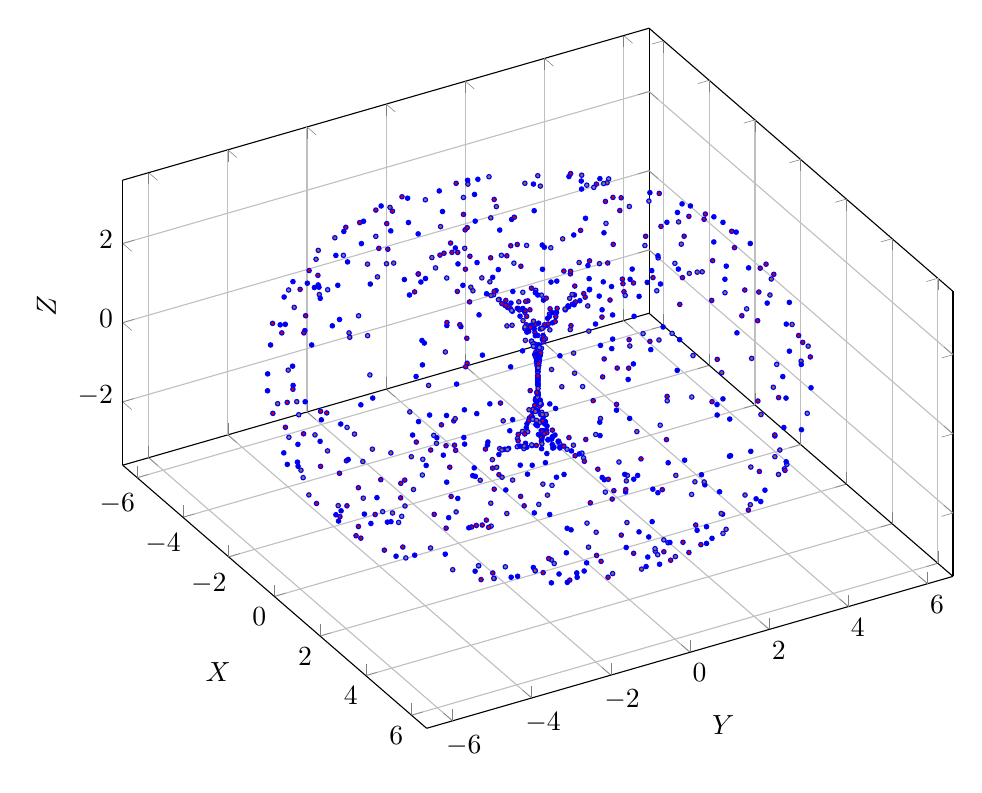
\begin{tikzpicture}
          \begin{axis}[
                view={60}{30},
                width=\textwidth, 
                axis equal,
                grid=major,
                xlabel={$X$},
                ylabel={$Y$},
                zlabel={$Z$},
        %        title={Random Points Inside a Horn Torus},
                samples=50,
                domain=0:360,
                y domain=0:360
            ]
            
            % Define parameters for a horn torus
            \pgfmathsetmacro{\R}{3}  % Major radius, set equal to minor radius
            \pgfmathsetmacro{\r}{3}  % Minor radius, set equal to major radius
            \pgfmathsetmacro{\thickness}{0.7} % Thickness to control the spread within the torus tube
        
            % Generate random points inside the horn torus
            \foreach \i in {1,...,888} {
                \pgfmathsetmacro{\theta}{random(0, 360)}
                \pgfmathsetmacro{\phi}{random(0, 360)}
                \pgfmathsetmacro{\radialDist}{\r + random(-\thickness, \thickness)}
                \pgfmathsetmacro{\x}{(\R + \radialDist * cos(\phi)) * cos(\theta)}
                \pgfmathsetmacro{\y}{(\R + \radialDist * cos(\phi)) * sin(\theta)}
                \pgfmathsetmacro{\z}{\radialDist * sin(\phi)}
        
                \addplot3+[only marks, mark=*, mark size=0.8pt, color=blue] coordinates {(\x, \y, \z)};
            }
            \end{axis}
        \end{tikzpicture}
    \caption[Horn Torus point cloud]{\textbf{Horn Torus point cloud.} Coded in to render in LaTeX with the help of ChatGPT $4$o.}
    \label{Wolfram Horn Torus}
\end{figure}
\clearpage



\section{The Data Visualisation Catalogue by Severino Ribecca}

\begin{figure}[h!]
    \centering
    \includegraphics[height=0.8\textheight]{figures/A.2.png}
    \caption[The Data Visualisation Catalogue]{\textbf{The Data Visualisation Catalogue.} 
\citep{ribecca_data_2017}. Used with Ribecca's permission.}
    \label{fig:A.2}
\end{figure}
\index[people]{Ribecca, Severino}
\clearpage

\section{Semantic Field \textit{S}}
\label{Appendix Semantic Field S}

In this section, I list the 310 terms of Semantic Field \textit{S}, as discussed in Chapter 5. To arrive at this list, I uploaded my thesis as a PDF to ChatGPT $4$o and parsed its keywords with the following prompt sequence: 
\begin{enumerate}
    \item[\textbf{1}] ``Categorize and list the key words in this document."
    \item[\textbf{2}] ``Write these as a list separated by commas, ranked by their relevance in the text"
\end{enumerate}

\rule{\linewidth}{0.4pt}


\begin{multicols}{4}
\begin{enumerate}[label=\arabic*.]
\item A Dish with One Spoon
\item abduction
\item Abundant Intelligences project
\item academic cross-pollination
\item academic knowledge management (AKM)
\item accessibility
\item Artificial General Intelligence (AGI)
\item AI energy consumption
\item algorithm
\item analogy
\item anti-oppression
\item Artificial Intelligence (AI)
\item axiological paradigms
\item biocultural memory
\item biodynamic agriculture
\item Blender
\item blind spots
\item Boundary Critique
\item capitalist extractivist economy
\item ChatGPT
\item Circle Semantic Shape
\item classification of natural forms
\item climate crisis
\item climate crisis mitigation
\item climate hyperobject
\item climate resilience
\item Carbon dioxide (CO2)
\item collaborative co-creation
\item collaborative Knowledge Production
\item colligative theory formation
\item complexity management
\item composition
\item Computational Analysis of Texts and Graphs (CATG)
\item Computational Graphesis
\item Computational Semiosis
\item conceptual gateways
\item Conceptual Graphs
\item Conceptual Networks
\item Cone Semantic Form
\item Cones of Plausibility
\item consilience
\item consilience across disciplines
\item Consilience in Knowledge Activation (CKA)
\item Consilience of Inductions
\item consolation
\item constellationary fields
\item conversational model
\item Creation-as-Research
\item Creative Presentations of Research
\item criminal justice system
\item Critical Systems Thinking (CST)
\item cybernetic mycelium
\item cybernetic rhizome
\item Cylinder Semantic Form
\item data activation
\item data hierarchy
\item data hierarchy visualization
\item data ontology modeling
\item data-information-knowledge-wisdom hierarchy (DIKW)
\item data-to-knowledge transformation
\item database of databases
\item decentralized knowledge structure
\item decomposition
\item deduction
\item degree-difference
\item Design for Health (DH)
\item Design for Sustainability Transitions (DfST)
\item Design with a Capital D
\item desolation
\item diagrammatic reasoning
\item Digital Humanities
\item dimensional addition
\item dimensionality
\item disciplinary interchange
\item discourse fields
\item domain models
\item double cone in optics
\item Double-Cone Semantic Form
\item double-diamond shape
\item eco-justice
\item ecoanthroposymbiosis
\item ecojustice
\item ecological cost of AI
\item ecologically informed AI strategy
\item Embedding Projector
\item energy resources
\item Entity-Relationship (ER) diagrams
\item environmental crisis
\item environmental degradation
\item environmental sustainability
\item epistemological diversity
\item Epistemology
\item Equity-Centered Community Design
\item Equity-Centered Community Design (ECCD)
\item ethnobotany
\item ethnoecology
\item Euclidean
\item evidence synthesis
\item filtration
\item formation and growth in morphology
\item funnel plot
\item futures cone
\item general consilience (GC)
\item Generous AI
\item geometric compositions
\item Gestalt psychology
\item gigamapping
\item glass box AI
\item Global Assortativity
\item Global Topological Synchronization (GTS)
\item GPT-3
\item GPT-4
\item graph embeddings
\item graph isomorphology
\item graph LLMs
\item graph morphology
\item graph of concepts
\item graph-based ontology models
\item graphesis
\item graphical user interface (GUI)
\item graphically structured knowledge
\item graphlet interface
\item graphlets
\item hierophanic
\item HITL (Human-in-the-Loop)
\item HITL CATG KA
\item Horn of Futures
\item Horn Torus Semantic Form
\item Human Analysis of Text and Graphs (HATG)
\item humanistic interface design
\item hyper-specialization
\item hyperlinked bibliometric graphing
\item hyperobject
\item incipit
\item Inclusive Design (ID)
\item induction
\item information design
\item information overload
\item information visualization
\item information visuospatialization
\item InfraNodus
\item interbeing
\item interdisciplinarity
\item interdisciplinary consilience
\item interdisciplinary Knowledge co-Production
\item interdisciplinary Knowledge Production
\item interdisciplinary synthesis
\item interdisciplinary topic mapping
\item Intergovernmental Panel on Climate Change (IPCC)
\item interpretable AI
\item isomorphic interbeing
\item isomorphogenesis
\item isomorphology
\item knowledge abstraction and synthesis
\item Knowledge Activation (KA)
\item knowledge design studio laboratory
\item knowledge engineering
\item knowledge graphs
\item Knowledge Management (KM)
\item Knowledge Production (KP)
\item Knowledge Production for Sustainability Transitions (KPST)
\item Knowledge Production through composition
\item Knowledge Production through visuospatial Semantic Form composition
\item Knowledge Pyramid
\item Knowledge Surfacing (KSu)
\item Knowledge Surfacing, Synthesis, Translation, and Creation(KSSTP)
\item Knowledge Synthesis (KSy)
\item Knowledge Translation (KT)
\item knowledge work platforms
\item KP quantification
\item Large Language Model (LLM)
\item logoi
\item logos of form
\item Logseq
\item Loop-line
\item Low-dimensional topology
\item ludic quality
\item major diameter
\item major radius
\item manual node placement
\item Markdown language
\item material infrastructure
\item Meru Chakra
\item meta-analysis
\item meta-language
\item meta-Systematic Combining (MSC)
\item metaphysics
\item methodological framework
\item methodological pluralism
\item middle ontology
\item minor diameter
\item minor radius
\item Mistral 7B
\item MNIST handwritten digits database
\item monocrops
\item morphology
\item moving spatial network graphs
\item multi-dimensional network graphs
\item multi-mathematical approach
\item multi-scale topological data features
\item natural resources
\item network graph
\item network graph composition
\item network graphlet
\item network subgraphs
\item networked data visualization
\item node grouping
\item Obsidian
\item Ontological Semantic Network Summaries (OSNS)
\item ontology
\item opaque AI
\item oppressive terminology
\item Oslo School of Systemic Design
\item outer diameter
\item outer radius
\item particle accelerator of ideas
\item Perceptual Artifacts Lab (PAL)
\item permaculture
\item Persistence Homology (PH)
\item Personal Knowledge Management (PKM)
\item perspective in art
\item plant-human co-evolution
\item point cloud
\item point plot heatmap
\item power relations
\item qualitative methods
\item Query Graphs
\item Query Isomorphs
\item rectangular coordinate system
\item Research-Creation
\item Research-for-Creation
\item Research-from-Creation
\item researcher grouping
\item rewilding
\item Ring Torus Semantic Form
\item Roam Research
\item Semantic Field S
\item Semantic Forms
\item semantic network mapping
\item Semantic Shapes
\item Semantic Topological Semiotics
\item simplicial complex
\item Small Language Models
\item social inequality
\item social justice
\item Social Sciences and Humanities Research Council
\item spatial and temporal modeling
\item spatial composition
\item spatial network graphs
\item spatial semiotic representation
\item spatial topic model network graphs
\item Sphere Semantic Form
\item Sri Yantra
\item stakeholder
\item Sustainability Transitions Knowledge Activation (STKA)
\item studio laboratory of knowledge design
\item surfaces of revolution
\item sustainability solutions frameworks
\item Sustainability Transitions (ST)
\item symbol composition
\item Symbol-setting
\item symbolic representation
\item syntopical consilience
\item Syntopical Consilience Abduction (SCA)
\item syntopical reading
\item Syntopicon
\item Systematic Combining (SC)
\item Systemic Design
\item Systemic Design Association (SDA)
\item Systems Oriented Design (SOD)
\item Systems Theory
\item Systems Thinking
\item Topological Capta Analysis (TCA)
\item TCA Researcher Grouping
\item TCA Workspace
\item tensors
\item Terroir of Text and Graphs (TTG)
\item text graphs
\item thought forms
\item thought signs
\item three-dimensional forms
\item three-dimensional information visualization
\item three-dimensional topic models
\item topic model network graphs
\item Topic Models
\item Topological Data Analysis (TDA)
\item Topological Capta Analysis (TCA)
\item topological semiotics
\item Topology
\item toroidal manifold
\item torus
\item transdisciplinary KA (Knowledge Activation)
\item Tree of Porphyry
\item UN Sustainable Development Goals (SDGs)
\item University
\item upper ontology
\item vector embeddings
\item vector search
\item Vedic visuospatial culture
\item visual argument
\item visual epistemology
\item visual reasoning
\item visuospatial epistemology
\item visuospatial forms of knowledge production
\item visuospatial knowledge activation interface
\item visuospatial reasoning
\item weighting
\item wicked problem
\item Zettelkasten
\item Zone of Semantic Stasis
\end{enumerate}
\end{multicols}
\clearpage

\section{Adler’s 102 \textit{Great Ideas}}
The following terms are listed alphabetically as per The \textit{Great Ideas: a Syntopicon of Great Books of the Western World} (1952), derived from the texts in \textit{Great Books of the Western World} (1952).
\begin{multicols}{4} % Use 2 or 3 columns, whichever fits well
\begin{enumerate}[label=\arabic*.]
    \item Angel
    \item Animal
    \item Aristocracy
    \item Art
    \item Astronomy and Cosmology
    \item Beauty
    \item Being
    \item Cause
    \item Chance
    \item Change
    \item Citizen
    \item Constitution
    \item Courage
    \item Custom and Convention
    \item Definition
    \item Democracy
    \item Desire
    \item Dialectic
    \item Duty
    \item Education
    \item Element
    \item Emotion
    \item Eternity
    \item Evolution
    \item Experience
    \item Family
    \item Fate
    \item Form
    \item God
    \item Good and Evil
    \item Government
    \item Habit
    \item Happiness
    \item History
    \item Honor
    \item Hypothesis
    \item Idea
    \item Immortality
    \item Induction
    \item Infinity
    \item Judgement
    \item Justice
    \item Knowledge
    \item Labor
    \item Language
    \item Law
    \item Liberty
    \item Life and Death
    \item Logic
    \item Love
    \item Man
    \item Mathematics
    \item Matter
    \item Mechanics
    \item Medicine
    \item Memory and Imagination
    \item Metaphysics
    \item Mind
    \item Monarch
    \item Nature
    \item Necessity and Contingency
    \item Oligarchy
    \item One and Many
    \item Opinion
    \item Opposition
    \item Philosophy
    \item Physics
    \item Pleasure and Pain
    \item Poetry
    \item Principle
    \item Progress
    \item Prophecy
    \item Prudence
    \item Punishment
    \item Quality
    \item Quantity
    \item Reasoning
    \item Relation
    \item Religion
    \item Revolution
    \item Rhetoric
    \item Same and Other
    \item Science
    \item Sense
    \item Sign and Symbol
    \item Sin
    \item Slavery
    \item Soul
    \item Space
    \item State
    \item Temperance
    \item Theology
    \item Time
    \item Truth
    \item Tyranny and Despotism
    \item Universal and Particular
    \item Virtue and Vice
    \item War and Peace
    \item Wealth
    \item Will
    \item Wisdom
    \item World
\end{enumerate}
\end{multicols} % Use 2 or 3 columns, whichever fits well
\clearpage


\section{Authors included in \textit{Great Books of the Western World} (1952)}
The \textit{Great Books of the Western World} (1952) includes works by the following authors:
\begin{multicols}{4}
\RaggedRight Homer\\
Aeschylus\\
Sophocles\\
Euripides\\
Aristophanes\\
Herodotus\\
Thucydides\\
Plato\\
Aristotle\\
Hippocrates\\
Galen\\
Euclid\\
Archimedes\\
Apollonius\\
Nichomachus\\
Lucretius\\
Epictetus\\
Marcus Aurelius\\
Virgil\\
Plutarch\\
Tacitus\\
Ptolemy\\
Copernicus\\
Kepler\\
Plotinus\\
Augustine\\
Thomas Aquinas\\
Dante\\
Chaucer\\
Machiavelli\\
Hobbes\\
Rabelais\\
Montaigne\\
Shakespeare\\
Gilbert\\
Galileo\\
Harvey\\
Cervantes\\
Francis Bacon\\
Descartes\\
Spinoza\\
Milton\\
Pascal\\
Newton\\
Huygens\\
Locke\\
Berkeley\\
Hume\\
Swift\\
Sterne\\
Fielding\\
Montesquieu\\
Rousseau\\
Adam Smith\\
Gibbon\\
Kant\\
J. S. Mill\\
Boswell\\
Lavoisier\\
Fourier\\
Faraday\\
Hegel\\
Goethe\\
Melville\\
Darwin\\
Marx\\
Engels\\
Tolstoy\\
Dostoyevsky\\
William James\\
Freud
\end{multicols}
\clearpage





\section{Categorizing the subjects of this thesis}
\raggedcolumns
\begin{multicols}{2}

\noindent\hangindent=1.5em \textbf{Computer Science} \\
Artificial Intelligence (AI) \\
Machine Learning \\
Natural Language Processing (NLP) \\
Computational Linguistics \\
Data Science \\
Human-Computer Interaction (HCI) \\
Information Retrieval \\
Knowledge Representation and Reasoning \\
Topological Data Analysis (TDA) \\
Graph Theory \\
\vspace{4mm}

\noindent\hangindent=1.5em \textbf{Mathematics} \\
Topology \\
Geometry \\
Computational Topology \\
Mathematical Modeling \\
\vspace{4mm}

\noindent\hangindent=1.5em \textbf{Philosophy} \\
Philosophy of Information \\
Philosophy of Language \\
Epistemology \\
Semiotics \\
Philosophy of Science \\
Ontology \\
\vspace{4mm}

\noindent\hangindent=1.5em \textbf{Cognitive Sciences} \\
Cognitive Psychology \\
Cognitive Neuroscience \\
Visual Cognition \\
Embodied Cognition \\
\vspace{4mm}

\noindent\hangindent=1.5em \textbf{Information Science} \\
Knowledge Management \\
Personal Knowledge Management (PKM) \\
Information Visualization \\
Library and Information Science \\
Ontologies \\
Digital Libraries \\
\vspace{4mm}

\noindent\hangindent=1.5em \textbf{Design} \\
Systems Oriented Design (SOD) \\
Systemic Design \\
Information Design \\
Visual Communication Design \\
Human-Centered Design \\
\vspace{4mm}

\noindent\hangindent=1.5em \textbf{Digital Humanities} \\
Computational Humanities \\
Digital Scholarship \\
Humanistic Interface Design \\
\vspace{4mm}

\noindent\hangindent=1.5em \textbf{Interdisciplinary Studies} \\
Sustainability Transitions \\
Environmental Studies \\
Climate Science \\
Ecojustice \\
Indigenous Studies \\
Decolonizing Methodologies \\
\vspace{4mm}

\noindent\hangindent=1.5em \textbf{Linguistics} \\
\RaggedRight Computational Linguistics \\
Semantics \\
Pragmatics \\
Language and Thought \\
\vspace{4mm}

\noindent\hangindent=1.5em \textbf{Education} \\
Knowledge Activation \\
Collaborative Learning \\
\RaggedRight Interdisciplinary Education \\
Educational Technology \\
\vspace{4mm}

\noindent\hangindent=1.5em \textbf{Sociology} \\
Sociology of Knowledge \\
Science and Technology Studies (STS) \\
Cultural Studies \\
\vspace{4mm}

\noindent\hangindent=1.5em \textbf{Communication Studies} \\
Media Studies \\
Information Theory \\
Symbolic Communication \\
\vspace{4mm}

\noindent\hangindent=1.5em \textbf{Ethnography and Anthropology} \\
Ethnoecology \\
Ethnobotany \\
Cultural Anthropology \\
\vspace{4mm}

\noindent\hangindent=1.5em \textbf{Visual Studies} \\
Visual Epistemology \\
Visual Reasoning \\
Visual Semiotics \\
Graphical Representation \\
\end{multicols}

\clearpage






\section{Experts consulted}
I acknowledge with professional admiration the subject matter experts who provided formative feedback for this thesis. I list their names here in alphabetical order by surname:

\begin{itemize}[label={}]
    \item \textbf{Dr. Evan Timothy Barba}, Associate Professor at Georgetown University
    \item \textbf{Tega Brain}, artist and Associate Professor at New York University (NYU)
    \item \textbf{Antionette D. Carroll}, founder of the Institute of Equitable Design and Justice, and Creative Reaction Labs
    \item \textbf{John P. Comer}, founder of Architects Of Justice; National Organizing Director of The Redress Movement
    \item \textbf{Dr.Peter Coppin}, Director of the The Perceptual Artifacts Lab (PAL) and  Associate Professor of Design at OCAD University. 
    \item \textbf{Dr. Sara Diamond}, OCAD University Research Chair, Director of the Visual Analytics Lab, and Co-investigator of the OCAD U Abundant Intelligences A Dish with One Spoon – Towards “Generous AI” Invention and Collaboration project
    \item \textbf{Dr. Michael Doser}, senior research physicist at the European Council for Nuclear Research/Conseil Européen pour la Recherche Nucléaire (CERN)
    \item \textbf{Balazs Farago}, founder and CEO of Walters Cube.
    \item \textbf{Ekaterina Grgurić}, Digital Scholarship Librarian at the University of British Columbia (UBC)
    \item \textbf{Michael Groenendyk}, Digital Scholarship Librarian at Concordia University
    \item \textbf{Micki Kaufman}, historian and digital scholar at the City University of New York
    \item \textbf{Dr. Peter Jones}, founder of the Strategic Innovation Lab, co-founder of the Systemic Design Association, and Distinguished Professor in Systemic Design for the School of Architecture, Art and Design at the Tecnológico de Monterrey
    \item \textbf{Amanda Licastro}, Digital Scholarship Librarian at Swarthmore College
    \item \textbf{Dr. Blake Madill}, Associate Professor of Pure Mathematics at the University of Waterloo
    \item \textbf{Cheryl May}, Executive Editor for the Systemic Design Association, and PhD candidate at London South Bank University
    \item \textbf{Dr. Gavin Mendel-Gleason}, CTO of TerminusDB, and former research fellow at Trinity College Dublin in the School of Statistics and Computer Science
    \item \textbf{Ola Mazzuca}, exhibition operations at the Gallery at Mason Studio
    \item \textbf{Antonio Muñoz Gomez}, Digital Scholarship Librarian at the University of Waterloo
    \item \textbf{Dr. Lennart Nacke}, University Research Chair and Professor at the University of Waterloo, and Associate Director of the Stratford School of Interaction Design and Business, and Director of the HCI Games Group at the University of Waterloo's Games Institute
    \item \textbf{Rahul Nayak}, data scientist from the Indian Institute of Technology
    \item \textbf{Dr. Dmitry Paranyushkin}, founder of InfraNodus and senior researcher at Nodus Labs
    \item \textbf{Dr. Paul Pangaro}, President of the American Society for Cybernetics
    \item \textbf{Dr. Michael J. Prokopow}, cultural historian, curator, and professor at OCAD University
    \item \textbf{Santiago Ortiz}, director of Moebio Labs
    \item \textbf{Ryan J. A. Murphy}, PhD candidate at the University of Newfoundland and Co-Secretary of the Systemic Design Association
    \item \textbf{Dr. Birger Sevaldson}, professor at the Oslo School of Architecture and Design, and at the University of South-Eastern Norway
    \item \textbf{Peter Scott}, lecturer at OCAD University
    \item \textbf{Dr. Maria Aleksandrovna Simakova}, Foucault scholar from the University of Toronto
    \item \textbf{Kirsta Stapelfeldt}, Associate Librarian, Research and Digital Initiatives at the University of Toronto Scarborough Digital Scholarship Unit
    \item \textbf{Brian Sunter}, software engineer from the University of Florida
    \item \textbf{Serkan Özkaya}, conceptual artist
    \item \textbf{David Kwasny}, Data and Digital Literacy Librarian at the University of Toronto Scarborough Digital Scholarship Unit
    \item \textbf{Kyle Winters}, CEO of NEXT Canada
\end{itemize}

\clearpage






\section{Research presentations}

In this section, I list the presentations I delivered about my work during my thesis research: \\

\begin{enumerate}


    \item[{2024}] \textit{Systems Oriented Disruptions}, presented for the annual International Innovation Forum hosted by the Strategic Foresight and Innovation program in the OCAD University School of Graduate Studies
 
    \item[{2024}] \textit{Systems Oriented Disruptions}, presented for Creative Disruptions// re-imagining our futures the graduate thesis exhibition by the Digital Futures program in the OCAD University’s School of Graduate Studies

    \item[{2024}]  \textit{Body of Aesthetics}, a panel discussion moderated by curator Sara Dagovic and joined by artist Artemis Han, The Gallery at Mason Studio, Toronto

    \item[{2023}] \textit{Three-dimensional plotting of information categories using P5.js}, Perceptual Artifacts Lab in OCAD University, moderated by the PAL Director Dr. Peter Coppin  

    \item[{2023}] \textit{Song Within a Sacrifice Zone}, presented for \textit{Uses and Abuses of Power in Alternative Spiritualities}, the annual conference by the Program for the Evolution of Spirituality in the Harvard Divinity School
 
    \item[{2023}] \textit{The biopower of faith leaders who are also alternative medicine practitioners in alternative spiritual communities}, presented for \textit{Uses and Abuses of Power in Alternative Spiritualities}, the annual conference by the Program for the Evolution of Spirituality in the Harvard Divinity School
 
    \item[{2023}] \textit{Knowledge Translation vs the Climate Crisis} presented for the annual colloquium hosted by the Digital Futures in the OCAD University School of Graduate Studies
 
    \item[{2022}] \textit{Dissonance}, presented for the Too Big To Fail Exhibition organized by the Interdisciplinary Master’s of Art, Media and Design in the OCAD University School of Graduate Studies

    \item[{2022}] \textit{Data Tori}, presented for the annual Graduate Colloquium, moderated by Duchamp scholar Dr. Julian Haladyn, in the OCAD University School of Graduate Studies

    \item[{2022}] \textit{Medicinallity of Symbol}, presented for the annual research panel organized by the Interdisciplinary Master’s of Art, Media and Design, in the OCAD University School of Graduate Studies, moderated by Graduate Program Director Jay Irizawa
    
\end{enumerate}
\clearpage




\section{Art exhibitions}

In this section, I list the art exhibitions in which I showcased my work during my thesis research: \\

\begin{enumerate}
    \item[{2024}] \textit{GradEx 109}, OCAD University

    \item[{2024}] \textit{Creative Disruptions// re-imagining our futures}, Digital Futures graduate thesis exhibition, OCAD University, Waterfront Campus. 
 
    \item[{2024}] \textit{Body of Aesthetics, curated by Sara Dagovic}, The Gallery at Mason Studio, Toronto

    \item[{2023}] \textit{Digital Futures Open Show}, OCAD University, School of Graduate Studies

    \item[{2023}] \textit{Song Within a Sacrifice Zone}, Harvard Divinity School, Swartz Hall
 
    \item[{2023}] \textit{Resilience and Connection: artistic explorations of mental health}, L.R. Wilson Building, McMaster University 
 
    \item[{2023}] \textit{Too Big to Fail}, Open Space Gallery, OCADU
 
    \item[{2022}] \textit{The Incomplete}, The Great Hall Gallery, OCADU
\end{enumerate}
\clearpage





\section{Resources and tools tested and used during thesis}
\label{Appendix Resources and Tools}
\begin{multicols}{2}

\noindent\hangindent=1.5em \textbf{Hardware} \\
Macbook Pro, 16-inch, 2021, Apple M1 Max, 32 GB RAM

\vspace{4mm}

\noindent\hangindent=1.5em \textbf{Source Management} \\
Zotero \\
\RaggedRight \hangindent=1.5em Zotero Better BibTex extension v 6.7.202 by Emiliano Heyns (to generate citation keys) \\
Zotero Connector Chrome extension \\

\vspace{4mm}

\noindent\hangindent=1.5em \textbf{Personal Knowledge Management (PKM)} \\
Obsidian \\
Logseq \\
Logseq PDF reader \\
Readwise Official Plugin v1.4.9 \\
Roam Research \\
\vspace{4mm}
\noindent\hangindent=1.5em \textbf{Three-Dimensional Forms} \\
Blender, node programming \\

\vspace{4mm}

\noindent\hangindent=1.5em \textbf{Document Drafting} \\
\RaggedRight \hangindent=1.5em Overleaf, Online LaTeX editor \\
\RaggedRight \hangindent=1.5em Dissertate, LaTeX dissertation template by Jordan Suchow \\
\RaggedRight \hangindent=1.5em Pandoc for populating Better BibTeX citation keys into in-sentence citation and list of references \\
Google Docs \\
Google Chrome extension DocsAfter Dark \\
Microsoft Word \\

\vspace{4mm}

\noindent\hangindent=1.5em \textbf{Document Reading} \\
Zotero PDF reader \\
ProQuest Ebook Central \\
The Internet Archive \\
Logseq PDF reader \\
Readwise \\
Readwise Reader \\
\RaggedRight \hangindent=1.5em Readwise Chrome extension (synced to Logseq and Obsidian) \\
Apple Photos Optical Character Recognition \\
Adobe Acrobat \\
Adobe Digital Editions \\

\vspace{4mm}

\noindent\hangindent=1.5em \textbf{Infinite Canvas Text Analysis Tools} \\
Miro \\
Scapple \\

\vspace{4mm}

\noindent\hangindent=1.5em \textbf{Text Graphing Tools} \\
InfraNodus \\
\RaggedRight \hangindent=1.5em InfraNodus Chrome extension for its 3D knowledge graph \\
MIT’s SIMILE Timeline widget, run on Zotero \\
Obsidian Canvas, core plugin \\ 
Obsidian Outline, core plugin \\
Obsidian Graph View, core plugin \\
\RaggedRight \hangindent=1.5em Obsidian 3D Graph v1.0.5, community plugin by Alexander Weichart \\
Python 3.8.12 \\
PiVis* \\
Pandas Dataframes* \\
NetworkX* \\
Voyant Tools \\
* Python libraries \\

\vspace{4mm}


\noindent\hangindent=1.5em \textbf{LLMs} \\
Mistral 7B Open Orca* \\
Zephyr* \\
Grammarly AI Writing Assistant \\
Claude 3.5 Sonnet \\
Google Gemini Advanced 1.5 Pro\\
Chat GPT 3.5 \\
Chat GPT 4 \\
Chat GPT 4 Turbo \\
Chat GPT $4$o \\
Chat GPT 4-mini \\
Chat GPT o1-preview \\
Chat GPT o1 \\
Chat GPT o1-mini \\
* set up using Ollama \\

\vspace{4mm}


\noindent\hangindent=1.5em \textbf{Image Management} \\
Apple Photos \\
Affinity \\
Affinity Designer \\
Affinity Publisher \\
Pinterest \\
QuickTime Player \\

\vspace{4mm}

\noindent\hangindent=1.5em \textbf{Audio and Video Production} \\
\RaggedRight Final Cut Pro \\ 
\RaggedRight Logic Pro \\

\vspace{4mm}

\noindent\hangindent=1.5em \textbf{Typefaces in Figures} \\
iA Writer Quattro S \\
Helvetica Neue \\
Arial Black \\
Avenir Next Condensed \\

\vspace{4mm}

\noindent\hangindent=1.5em \textbf{Typefaces in Document} \\
Lato - used for text captions \\
Noto Mono - used for code \\
EB Garramond - used for all other text \\

\end{multicols}

\clearpage

%\chapter*{Indices}
%\addcontentsline{toc}{chapter}{Indices}
%\label{Index}




%\end{appendices} 
%<<<



%Testing >>>
\appendix
\renewcommand{\thechapter}{\Alph{chapter}} % Use letters for appendix chapters
\setcounter{chapter}{0} % Ensure numbering starts at 'A'

\chapter{Appendix Title 1}
\chapter[Appendices] {Appendices}
\label{Appendix}

\section{Thesis website}
\label{Appendix: Thesis website}
The ongoing developments of this thesis research and a gallery of moving Semantic Form models are available on the following website: 

\url{https://orusmateo.com/thesis-what-may-be-known-2025}

\section{LaTeX manuscript repository}
\label{LaTeX GitHub}
The following web page provides access to the LaTeX code used to compile this thesis, including all figures and formatting details:

\url{https://github.com/orusmateo/Orus-MA-Thesis}

\section{Moving and interactive models}
The following web page provides access to the moving and interactive models which I developed for my thesis. 

\url{https://orusmateo.com/moving-semantic-forms}

\section{Semantic Forms surface and volume equations }
\label{Semantic Forms equations}
The following table shows the volume and surface equations of the Semantic Forms' core geometries. 
\begin{table}[h]
    \centering
    \begin{tabular}{|l|l|l|}
\hline
 & \textit{Volume (V)} & \textit{Surface (S)} \\[10pt]
 \hline
cone &  $\pi r^2 \frac{h}{3}$ & $\pi r \sqrt{r^2+h^2}$  \\[10pt] \hline
 cylinder & $\pi r^2 h$ & $2 \pi r h$ \\[10pt]
  \hline
sphere & $\frac{4}{3} \pi  R^3$ & $4 \pi r^2$ \\[10pt] \hline
horn torus & $2 \pi^2 a^3$ & $4 \pi^2 a^2$ \\[10pt] \hline
ring torus & $\frac{1}{4} \pi^2(R+r)(R-r) a^*$ & $\pi^2 (R+r)(R-r)$ \\[10pt]
\hline
\multicolumn{3}{l}

    \end{tabular}
    %\caption{Caption}
\end{table}

\begin{quote}
    \centering *Pappus’s centroid theorem \citep{weisstein_torus_nodate}.
\end{quote}

\index[people]{Pappus}
\clearpage

\section{Application of Sarajlić et al. configurations to three-dimensional graphlets}
As part of my style guide for Query Isomorphs analysis, I propose that the Sarajlić et al. graphlet configurations \citep[p. 3]{sarajlic_graphlet-based_2016} can be used for graph input and graph analysis.

\begin{figure}[h!]
    \centering
    \includegraphics[width=0.8\textwidth]{figures/5.6.png}
    \caption[Example Query Isomorph in two dimensions and three dimensions assembled from directed graphlets]{\textbf{Example Query Isomorph in two dimensions and three dimensions assembled from directed graphlets.} \\
(a) From Sarajlić et al. 2016’s point b, “Illustration of how directed graphlets assemble together to form complex networks”, from “Figure 1. Illustration of directed graphlets” \citep[p. 3]{sarajlic_graphlet-based_2016}. In keeping with Sarajlić et al., the whole network can be created by adding graphlets G4, G1, and G3, meaning that in the process, a new graphlet, G2, was created. The colours red, green, blue, and black are sourced from \citep[p. 3]{sarajlic_graphlet-based_2016}. (b) Spatial arrangement adds the semantic affordance of verticality to communicate hierarchy of the blue node. Red nodes are querying for nodes in both higher and lateral hierarchies. (c) Other arrangements can easily facilitate different relationships in the Query Isomorph. (b) and (c) The colours red, green, and blue are sourced from \citep[p. 3]{sarajlic_graphlet-based_2016} here also, but white is used instead of black for contrast. Black nodes in this example are all placed in a lateral level of hierarchy. In a functional Query Isomorph platform, nodes could also be placed higher or lower than each other. Furthermore, the angles and directions of these graphlets are presented for simplicity of the variety they can have but do not represent the diversity of angles and forms that graphlets can be configured in as Query Isomorphs. 
}
    \label{f5.6}
\end{figure}
\clearpage


\section{The Semantic Forms located in Bertin’s taxonomy of network graphs}
\begin{figure}[h!]
    \centering
    \includegraphics[width=0.9\textwidth]{figures/A.3.png}
    \caption[Groups of imposition and types of imposition]{\textbf{Groups of imposition and types of imposition} \citep[p. 52]{bertin_semiology_2011}.
From \textit{Semiology of Graphics: Diagrams, Networks, Maps} by Jacques Bertin, translated by William J. Berg. Reprinted by permission of the University of Wisconsin Press. © 1983 by the Board of Regents of the University of Wisconsin System. All rights reserved.}
    \label{fig:A3}
\end{figure}
\index[people]{Bertin, Jacques}
\index[people]{Berg, William J.}
%\clearpage
\begin{figure}[h!]
    \centering
    \includegraphics[width=\textwidth]{figures/A.4.png}
    \caption[Groups of imposition and types of imposition as categories for my Semantic Shapes, Semantic Forms, and three-dimensional gigamaps]{\textbf{Groups of imposition and types of imposition as categories for my Semantic Shapes, Semantic Forms, and three-dimensional gigamaps}. My work is overlaid onto Bertin’s categorization of network diagrams \citep[p. 52]{bertin_semiology_2011} from \textit{Semiology of Graphics: Diagrams, Networks, Maps} by Jacques Bertin, translated by William J. Berg. Reprinted by permission of the University of Wisconsin Press. © 1983 by the Board of Regents of the University of Wisconsin System. All rights reserved.}
    \label{fig:A4}
\end{figure}
\index[people]{Bertin, Jacques}
\index[people]{Berg, William J.}
%\clearpage
\begin{figure}[h!]
    \centering
    \includegraphics[height=0.8\textheight]{figures/A.5.png}
    \caption[Implantation and imposition of network diagrams]{\textbf{Implantation and imposition of network diagrams} \citep[p. 270]{bertin_semiology_2011} \\
From \textit{Semiology of Graphics: Diagrams, Networks, Maps} by Jacques Bertin, translated by William J. Berg. Reprinted by permission of the University of Wisconsin Press. © 1983 by the Board of Regents of the University of Wisconsin System. All rights reserved.}
    \label{fig:A5}
\end{figure}
\index[people]{Bertin, Jacques}
\index[people]{Berg, William J.}
\begin{figure}[h!]
    \centering
    \includegraphics[width=\textwidth]{figures/A.6.png}
    \caption[Implantation and imposition of network diagrams as categories for my Semantic Shapes, Semantic Forms, and three-dimensional gigamaps]{\textbf{Implantation and imposition of network diagrams as categories for my Semantic Shapes, Semantic Forms, and three-dimensional gigamaps.} \citep[p. 270]{bertin_semiology_2011} 
My work is overlaid onto Bertin’s categorization of network diagrams \citep[p. 270]{bertin_semiology_2011} from \textit{Semiology of Graphics: Diagrams, Networks, Maps} by Jacques Bertin, translated by William J. Berg. Reprinted by permission of the University of Wisconsin Press. © 1983 by the Board of Regents of the University of Wisconsin System. All rights reserved.
}
    \label{fig:A6}
\end{figure}
\index[people]{Bertin, Jacques}
\index[people]{Berg, William J.}
\clearpage


\section{Graphical abstract of this thesis}
\begin{figure}[h!]
    \centering
    \includegraphics[width=\textwidth]{figures/AF1.pdf}
    \caption[Graphical abstract]{\textbf{Graphical abstract of this thesis}}
    \label{fig:graphical_abstract}
 \clearpage
\end{figure}
\clearpage


\section{Horn of futures}
\FloatBarrier
\begin{figure}[h!]
    \centering
    \includegraphics[width=\textwidth]{figures/5.29.png}
    \caption[Horn of Futures]{\textbf{Horn of Futures.} This figure depicts the 2D dimensional reduction of the bottom view of a modified 3D Cone of Plausibility \citetext{\citealp[p. 73]{bezold_overview_1993}; \citealp[p. 14]{taylor_creating_1990}}. This Cone Semantic Form is curved into a spiral similar to \autoref{fig:18} “Diagram of a design process with iterations” \citetext{\citealp[p. 343]{sevaldson_designing_2022}; \citealp{sevaldson_designing_2022-1}}. The 3D version of this form twists like a ram’s horn, and this thesis involves the study of the horn torus, hence the name \textit{Horn of Futures}. To represent Possible futures, the widest spiralling area is represented with a black colour, Plausible futures in dark grey, Probable futures in light grey, and Preferable futures is shown as a beige deviation from the Probable futures. The middle of the Preferable futures range is labelled with a green through-line, and the middle of the light grey Probable range is labelled with a red through-line.}
    \label{f5.29}
\end{figure}
\FloatBarrier
\clearpage







\section{Horn Torus point cloud}
\begin{figure}[h!]
    \centering
        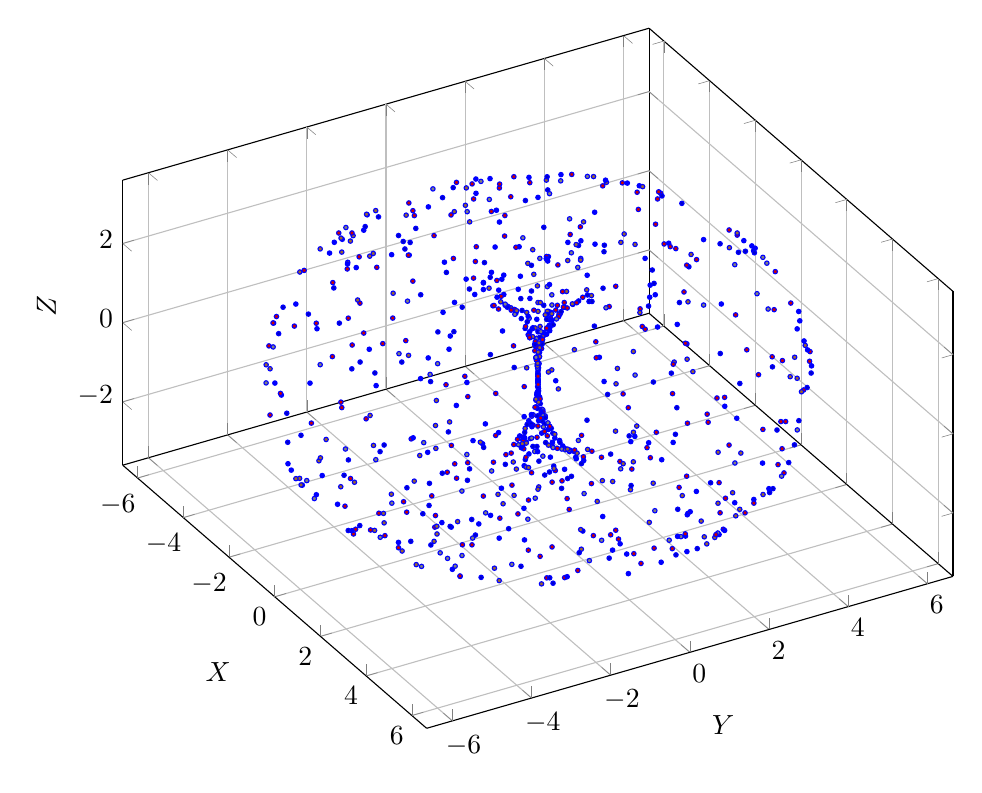
\begin{tikzpicture}
          \begin{axis}[
                view={60}{30},
                width=\textwidth, 
                axis equal,
                grid=major,
                xlabel={$X$},
                ylabel={$Y$},
                zlabel={$Z$},
        %        title={Random Points Inside a Horn Torus},
                samples=50,
                domain=0:360,
                y domain=0:360
            ]
            
            % Define parameters for a horn torus
            \pgfmathsetmacro{\R}{3}  % Major radius, set equal to minor radius
            \pgfmathsetmacro{\r}{3}  % Minor radius, set equal to major radius
            \pgfmathsetmacro{\thickness}{0.7} % Thickness to control the spread within the torus tube
        
            % Generate random points inside the horn torus
            \foreach \i in {1,...,888} {
                \pgfmathsetmacro{\theta}{random(0, 360)}
                \pgfmathsetmacro{\phi}{random(0, 360)}
                \pgfmathsetmacro{\radialDist}{\r + random(-\thickness, \thickness)}
                \pgfmathsetmacro{\x}{(\R + \radialDist * cos(\phi)) * cos(\theta)}
                \pgfmathsetmacro{\y}{(\R + \radialDist * cos(\phi)) * sin(\theta)}
                \pgfmathsetmacro{\z}{\radialDist * sin(\phi)}
        
                \addplot3+[only marks, mark=*, mark size=0.8pt, color=blue] coordinates {(\x, \y, \z)};
            }
            \end{axis}
        \end{tikzpicture}
    \caption[Horn Torus point cloud]{\textbf{Horn Torus point cloud.} Coded in to render in LaTeX with the help of ChatGPT $4$o.}
    \label{Wolfram Horn Torus}
\end{figure}
\clearpage



\section{The Data Visualisation Catalogue by Severino Ribecca}

\begin{figure}[h!]
    \centering
    \includegraphics[height=0.8\textheight]{figures/A.2.png}
    \caption[The Data Visualisation Catalogue]{\textbf{The Data Visualisation Catalogue.} 
\citep{ribecca_data_2017}. Used with Ribecca's permission.}
    \label{fig:A.2}
\end{figure}
\index[people]{Ribecca, Severino}
\clearpage

\section{Semantic Field \textit{S}}
\label{Appendix Semantic Field S}

In this section, I list the 310 terms of Semantic Field \textit{S}, as discussed in Chapter 5. To arrive at this list, I uploaded my thesis as a PDF to ChatGPT $4$o and parsed its keywords with the following prompt sequence: 
\begin{enumerate}
    \item[\textbf{1}] ``Categorize and list the key words in this document."
    \item[\textbf{2}] ``Write these as a list separated by commas, ranked by their relevance in the text"
\end{enumerate}

\rule{\linewidth}{0.4pt}


\begin{multicols}{4}
\begin{enumerate}[label=\arabic*.]
\item A Dish with One Spoon
\item abduction
\item Abundant Intelligences project
\item academic cross-pollination
\item academic knowledge management (AKM)
\item accessibility
\item Artificial General Intelligence (AGI)
\item AI energy consumption
\item algorithm
\item analogy
\item anti-oppression
\item Artificial Intelligence (AI)
\item axiological paradigms
\item biocultural memory
\item biodynamic agriculture
\item Blender
\item blind spots
\item Boundary Critique
\item capitalist extractivist economy
\item ChatGPT
\item Circle Semantic Shape
\item classification of natural forms
\item climate crisis
\item climate crisis mitigation
\item climate hyperobject
\item climate resilience
\item Carbon dioxide (CO2)
\item collaborative co-creation
\item collaborative Knowledge Production
\item colligative theory formation
\item complexity management
\item composition
\item Computational Analysis of Texts and Graphs (CATG)
\item Computational Graphesis
\item Computational Semiosis
\item conceptual gateways
\item Conceptual Graphs
\item Conceptual Networks
\item Cone Semantic Form
\item Cones of Plausibility
\item consilience
\item consilience across disciplines
\item Consilience in Knowledge Activation (CKA)
\item Consilience of Inductions
\item consolation
\item constellationary fields
\item conversational model
\item Creation-as-Research
\item Creative Presentations of Research
\item criminal justice system
\item Critical Systems Thinking (CST)
\item cybernetic mycelium
\item cybernetic rhizome
\item Cylinder Semantic Form
\item data activation
\item data hierarchy
\item data hierarchy visualization
\item data ontology modeling
\item data-information-knowledge-wisdom hierarchy (DIKW)
\item data-to-knowledge transformation
\item database of databases
\item decentralized knowledge structure
\item decomposition
\item deduction
\item degree-difference
\item Design for Health (DH)
\item Design for Sustainability Transitions (DfST)
\item Design with a Capital D
\item desolation
\item diagrammatic reasoning
\item Digital Humanities
\item dimensional addition
\item dimensionality
\item disciplinary interchange
\item discourse fields
\item domain models
\item double cone in optics
\item Double-Cone Semantic Form
\item double-diamond shape
\item eco-justice
\item ecoanthroposymbiosis
\item ecojustice
\item ecological cost of AI
\item ecologically informed AI strategy
\item Embedding Projector
\item energy resources
\item Entity-Relationship (ER) diagrams
\item environmental crisis
\item environmental degradation
\item environmental sustainability
\item epistemological diversity
\item Epistemology
\item Equity-Centered Community Design
\item Equity-Centered Community Design (ECCD)
\item ethnobotany
\item ethnoecology
\item Euclidean
\item evidence synthesis
\item filtration
\item formation and growth in morphology
\item funnel plot
\item futures cone
\item general consilience (GC)
\item Generous AI
\item geometric compositions
\item Gestalt psychology
\item gigamapping
\item glass box AI
\item Global Assortativity
\item Global Topological Synchronization (GTS)
\item GPT-3
\item GPT-4
\item graph embeddings
\item graph isomorphology
\item graph LLMs
\item graph morphology
\item graph of concepts
\item graph-based ontology models
\item graphesis
\item graphical user interface (GUI)
\item graphically structured knowledge
\item graphlet interface
\item graphlets
\item hierophanic
\item HITL (Human-in-the-Loop)
\item HITL CATG KA
\item Horn of Futures
\item Horn Torus Semantic Form
\item Human Analysis of Text and Graphs (HATG)
\item humanistic interface design
\item hyper-specialization
\item hyperlinked bibliometric graphing
\item hyperobject
\item incipit
\item Inclusive Design (ID)
\item induction
\item information design
\item information overload
\item information visualization
\item information visuospatialization
\item InfraNodus
\item interbeing
\item interdisciplinarity
\item interdisciplinary consilience
\item interdisciplinary Knowledge co-Production
\item interdisciplinary Knowledge Production
\item interdisciplinary synthesis
\item interdisciplinary topic mapping
\item Intergovernmental Panel on Climate Change (IPCC)
\item interpretable AI
\item isomorphic interbeing
\item isomorphogenesis
\item isomorphology
\item knowledge abstraction and synthesis
\item Knowledge Activation (KA)
\item knowledge design studio laboratory
\item knowledge engineering
\item knowledge graphs
\item Knowledge Management (KM)
\item Knowledge Production (KP)
\item Knowledge Production for Sustainability Transitions (KPST)
\item Knowledge Production through composition
\item Knowledge Production through visuospatial Semantic Form composition
\item Knowledge Pyramid
\item Knowledge Surfacing (KSu)
\item Knowledge Surfacing, Synthesis, Translation, and Creation(KSSTP)
\item Knowledge Synthesis (KSy)
\item Knowledge Translation (KT)
\item knowledge work platforms
\item KP quantification
\item Large Language Model (LLM)
\item logoi
\item logos of form
\item Logseq
\item Loop-line
\item Low-dimensional topology
\item ludic quality
\item major diameter
\item major radius
\item manual node placement
\item Markdown language
\item material infrastructure
\item Meru Chakra
\item meta-analysis
\item meta-language
\item meta-Systematic Combining (MSC)
\item metaphysics
\item methodological framework
\item methodological pluralism
\item middle ontology
\item minor diameter
\item minor radius
\item Mistral 7B
\item MNIST handwritten digits database
\item monocrops
\item morphology
\item moving spatial network graphs
\item multi-dimensional network graphs
\item multi-mathematical approach
\item multi-scale topological data features
\item natural resources
\item network graph
\item network graph composition
\item network graphlet
\item network subgraphs
\item networked data visualization
\item node grouping
\item Obsidian
\item Ontological Semantic Network Summaries (OSNS)
\item ontology
\item opaque AI
\item oppressive terminology
\item Oslo School of Systemic Design
\item outer diameter
\item outer radius
\item particle accelerator of ideas
\item Perceptual Artifacts Lab (PAL)
\item permaculture
\item Persistence Homology (PH)
\item Personal Knowledge Management (PKM)
\item perspective in art
\item plant-human co-evolution
\item point cloud
\item point plot heatmap
\item power relations
\item qualitative methods
\item Query Graphs
\item Query Isomorphs
\item rectangular coordinate system
\item Research-Creation
\item Research-for-Creation
\item Research-from-Creation
\item researcher grouping
\item rewilding
\item Ring Torus Semantic Form
\item Roam Research
\item Semantic Field S
\item Semantic Forms
\item semantic network mapping
\item Semantic Shapes
\item Semantic Topological Semiotics
\item simplicial complex
\item Small Language Models
\item social inequality
\item social justice
\item Social Sciences and Humanities Research Council
\item spatial and temporal modeling
\item spatial composition
\item spatial network graphs
\item spatial semiotic representation
\item spatial topic model network graphs
\item Sphere Semantic Form
\item Sri Yantra
\item stakeholder
\item Sustainability Transitions Knowledge Activation (STKA)
\item studio laboratory of knowledge design
\item surfaces of revolution
\item sustainability solutions frameworks
\item Sustainability Transitions (ST)
\item symbol composition
\item Symbol-setting
\item symbolic representation
\item syntopical consilience
\item Syntopical Consilience Abduction (SCA)
\item syntopical reading
\item Syntopicon
\item Systematic Combining (SC)
\item Systemic Design
\item Systemic Design Association (SDA)
\item Systems Oriented Design (SOD)
\item Systems Theory
\item Systems Thinking
\item Topological Capta Analysis (TCA)
\item TCA Researcher Grouping
\item TCA Workspace
\item tensors
\item Terroir of Text and Graphs (TTG)
\item text graphs
\item thought forms
\item thought signs
\item three-dimensional forms
\item three-dimensional information visualization
\item three-dimensional topic models
\item topic model network graphs
\item Topic Models
\item Topological Data Analysis (TDA)
\item Topological Capta Analysis (TCA)
\item topological semiotics
\item Topology
\item toroidal manifold
\item torus
\item transdisciplinary KA (Knowledge Activation)
\item Tree of Porphyry
\item UN Sustainable Development Goals (SDGs)
\item University
\item upper ontology
\item vector embeddings
\item vector search
\item Vedic visuospatial culture
\item visual argument
\item visual epistemology
\item visual reasoning
\item visuospatial epistemology
\item visuospatial forms of knowledge production
\item visuospatial knowledge activation interface
\item visuospatial reasoning
\item weighting
\item wicked problem
\item Zettelkasten
\item Zone of Semantic Stasis
\end{enumerate}
\end{multicols}
\clearpage

\section{Adler’s 102 \textit{Great Ideas}}
The following terms are listed alphabetically as per The \textit{Great Ideas: a Syntopicon of Great Books of the Western World} (1952), derived from the texts in \textit{Great Books of the Western World} (1952).
\begin{multicols}{4} % Use 2 or 3 columns, whichever fits well
\begin{enumerate}[label=\arabic*.]
    \item Angel
    \item Animal
    \item Aristocracy
    \item Art
    \item Astronomy and Cosmology
    \item Beauty
    \item Being
    \item Cause
    \item Chance
    \item Change
    \item Citizen
    \item Constitution
    \item Courage
    \item Custom and Convention
    \item Definition
    \item Democracy
    \item Desire
    \item Dialectic
    \item Duty
    \item Education
    \item Element
    \item Emotion
    \item Eternity
    \item Evolution
    \item Experience
    \item Family
    \item Fate
    \item Form
    \item God
    \item Good and Evil
    \item Government
    \item Habit
    \item Happiness
    \item History
    \item Honor
    \item Hypothesis
    \item Idea
    \item Immortality
    \item Induction
    \item Infinity
    \item Judgement
    \item Justice
    \item Knowledge
    \item Labor
    \item Language
    \item Law
    \item Liberty
    \item Life and Death
    \item Logic
    \item Love
    \item Man
    \item Mathematics
    \item Matter
    \item Mechanics
    \item Medicine
    \item Memory and Imagination
    \item Metaphysics
    \item Mind
    \item Monarch
    \item Nature
    \item Necessity and Contingency
    \item Oligarchy
    \item One and Many
    \item Opinion
    \item Opposition
    \item Philosophy
    \item Physics
    \item Pleasure and Pain
    \item Poetry
    \item Principle
    \item Progress
    \item Prophecy
    \item Prudence
    \item Punishment
    \item Quality
    \item Quantity
    \item Reasoning
    \item Relation
    \item Religion
    \item Revolution
    \item Rhetoric
    \item Same and Other
    \item Science
    \item Sense
    \item Sign and Symbol
    \item Sin
    \item Slavery
    \item Soul
    \item Space
    \item State
    \item Temperance
    \item Theology
    \item Time
    \item Truth
    \item Tyranny and Despotism
    \item Universal and Particular
    \item Virtue and Vice
    \item War and Peace
    \item Wealth
    \item Will
    \item Wisdom
    \item World
\end{enumerate}
\end{multicols} % Use 2 or 3 columns, whichever fits well
\clearpage


\section{Authors included in \textit{Great Books of the Western World} (1952)}
The \textit{Great Books of the Western World} (1952) includes works by the following authors:
\begin{multicols}{4}
\RaggedRight Homer\\
Aeschylus\\
Sophocles\\
Euripides\\
Aristophanes\\
Herodotus\\
Thucydides\\
Plato\\
Aristotle\\
Hippocrates\\
Galen\\
Euclid\\
Archimedes\\
Apollonius\\
Nichomachus\\
Lucretius\\
Epictetus\\
Marcus Aurelius\\
Virgil\\
Plutarch\\
Tacitus\\
Ptolemy\\
Copernicus\\
Kepler\\
Plotinus\\
Augustine\\
Thomas Aquinas\\
Dante\\
Chaucer\\
Machiavelli\\
Hobbes\\
Rabelais\\
Montaigne\\
Shakespeare\\
Gilbert\\
Galileo\\
Harvey\\
Cervantes\\
Francis Bacon\\
Descartes\\
Spinoza\\
Milton\\
Pascal\\
Newton\\
Huygens\\
Locke\\
Berkeley\\
Hume\\
Swift\\
Sterne\\
Fielding\\
Montesquieu\\
Rousseau\\
Adam Smith\\
Gibbon\\
Kant\\
J. S. Mill\\
Boswell\\
Lavoisier\\
Fourier\\
Faraday\\
Hegel\\
Goethe\\
Melville\\
Darwin\\
Marx\\
Engels\\
Tolstoy\\
Dostoyevsky\\
William James\\
Freud
\end{multicols}
\clearpage





\section{Categorizing the subjects of this thesis}
\raggedcolumns
\begin{multicols}{2}

\noindent\hangindent=1.5em \textbf{Computer Science} \\
Artificial Intelligence (AI) \\
Machine Learning \\
Natural Language Processing (NLP) \\
Computational Linguistics \\
Data Science \\
Human-Computer Interaction (HCI) \\
Information Retrieval \\
Knowledge Representation and Reasoning \\
Topological Data Analysis (TDA) \\
Graph Theory \\
\vspace{4mm}

\noindent\hangindent=1.5em \textbf{Mathematics} \\
Topology \\
Geometry \\
Computational Topology \\
Mathematical Modeling \\
\vspace{4mm}

\noindent\hangindent=1.5em \textbf{Philosophy} \\
Philosophy of Information \\
Philosophy of Language \\
Epistemology \\
Semiotics \\
Philosophy of Science \\
Ontology \\
\vspace{4mm}

\noindent\hangindent=1.5em \textbf{Cognitive Sciences} \\
Cognitive Psychology \\
Cognitive Neuroscience \\
Visual Cognition \\
Embodied Cognition \\
\vspace{4mm}

\noindent\hangindent=1.5em \textbf{Information Science} \\
Knowledge Management \\
Personal Knowledge Management (PKM) \\
Information Visualization \\
Library and Information Science \\
Ontologies \\
Digital Libraries \\
\vspace{4mm}

\noindent\hangindent=1.5em \textbf{Design} \\
Systems Oriented Design (SOD) \\
Systemic Design \\
Information Design \\
Visual Communication Design \\
Human-Centered Design \\
\vspace{4mm}

\noindent\hangindent=1.5em \textbf{Digital Humanities} \\
Computational Humanities \\
Digital Scholarship \\
Humanistic Interface Design \\
\vspace{4mm}

\noindent\hangindent=1.5em \textbf{Interdisciplinary Studies} \\
Sustainability Transitions \\
Environmental Studies \\
Climate Science \\
Ecojustice \\
Indigenous Studies \\
Decolonizing Methodologies \\
\vspace{4mm}

\noindent\hangindent=1.5em \textbf{Linguistics} \\
\RaggedRight Computational Linguistics \\
Semantics \\
Pragmatics \\
Language and Thought \\
\vspace{4mm}

\noindent\hangindent=1.5em \textbf{Education} \\
Knowledge Activation \\
Collaborative Learning \\
\RaggedRight Interdisciplinary Education \\
Educational Technology \\
\vspace{4mm}

\noindent\hangindent=1.5em \textbf{Sociology} \\
Sociology of Knowledge \\
Science and Technology Studies (STS) \\
Cultural Studies \\
\vspace{4mm}

\noindent\hangindent=1.5em \textbf{Communication Studies} \\
Media Studies \\
Information Theory \\
Symbolic Communication \\
\vspace{4mm}

\noindent\hangindent=1.5em \textbf{Ethnography and Anthropology} \\
Ethnoecology \\
Ethnobotany \\
Cultural Anthropology \\
\vspace{4mm}

\noindent\hangindent=1.5em \textbf{Visual Studies} \\
Visual Epistemology \\
Visual Reasoning \\
Visual Semiotics \\
Graphical Representation \\
\end{multicols}

\clearpage






\section{Experts consulted}
I acknowledge with professional admiration the subject matter experts who provided formative feedback for this thesis. I list their names here in alphabetical order by surname:

\begin{itemize}[label={}]
    \item \textbf{Dr. Evan Timothy Barba}, Associate Professor at Georgetown University
    \item \textbf{Tega Brain}, artist and Associate Professor at New York University (NYU)
    \item \textbf{Antionette D. Carroll}, founder of the Institute of Equitable Design and Justice, and Creative Reaction Labs
    \item \textbf{John P. Comer}, founder of Architects Of Justice; National Organizing Director of The Redress Movement
    \item \textbf{Dr.Peter Coppin}, Director of the The Perceptual Artifacts Lab (PAL) and  Associate Professor of Design at OCAD University. 
    \item \textbf{Dr. Sara Diamond}, OCAD University Research Chair, Director of the Visual Analytics Lab, and Co-investigator of the OCAD U Abundant Intelligences A Dish with One Spoon – Towards “Generous AI” Invention and Collaboration project
    \item \textbf{Dr. Michael Doser}, senior research physicist at the European Council for Nuclear Research/Conseil Européen pour la Recherche Nucléaire (CERN)
    \item \textbf{Balazs Farago}, founder and CEO of Walters Cube.
    \item \textbf{Ekaterina Grgurić}, Digital Scholarship Librarian at the University of British Columbia (UBC)
    \item \textbf{Michael Groenendyk}, Digital Scholarship Librarian at Concordia University
    \item \textbf{Micki Kaufman}, historian and digital scholar at the City University of New York
    \item \textbf{Dr. Peter Jones}, founder of the Strategic Innovation Lab, co-founder of the Systemic Design Association, and Distinguished Professor in Systemic Design for the School of Architecture, Art and Design at the Tecnológico de Monterrey
    \item \textbf{Amanda Licastro}, Digital Scholarship Librarian at Swarthmore College
    \item \textbf{Dr. Blake Madill}, Associate Professor of Pure Mathematics at the University of Waterloo
    \item \textbf{Cheryl May}, Executive Editor for the Systemic Design Association, and PhD candidate at London South Bank University
    \item \textbf{Dr. Gavin Mendel-Gleason}, CTO of TerminusDB, and former research fellow at Trinity College Dublin in the School of Statistics and Computer Science
    \item \textbf{Ola Mazzuca}, exhibition operations at the Gallery at Mason Studio
    \item \textbf{Antonio Muñoz Gomez}, Digital Scholarship Librarian at the University of Waterloo
    \item \textbf{Dr. Lennart Nacke}, University Research Chair and Professor at the University of Waterloo, and Associate Director of the Stratford School of Interaction Design and Business, and Director of the HCI Games Group at the University of Waterloo's Games Institute
    \item \textbf{Rahul Nayak}, data scientist from the Indian Institute of Technology
    \item \textbf{Dr. Dmitry Paranyushkin}, founder of InfraNodus and senior researcher at Nodus Labs
    \item \textbf{Dr. Paul Pangaro}, President of the American Society for Cybernetics
    \item \textbf{Dr. Michael J. Prokopow}, cultural historian, curator, and professor at OCAD University
    \item \textbf{Santiago Ortiz}, director of Moebio Labs
    \item \textbf{Ryan J. A. Murphy}, PhD candidate at the University of Newfoundland and Co-Secretary of the Systemic Design Association
    \item \textbf{Dr. Birger Sevaldson}, professor at the Oslo School of Architecture and Design, and at the University of South-Eastern Norway
    \item \textbf{Peter Scott}, lecturer at OCAD University
    \item \textbf{Dr. Maria Aleksandrovna Simakova}, Foucault scholar from the University of Toronto
    \item \textbf{Kirsta Stapelfeldt}, Associate Librarian, Research and Digital Initiatives at the University of Toronto Scarborough Digital Scholarship Unit
    \item \textbf{Brian Sunter}, software engineer from the University of Florida
    \item \textbf{Serkan Özkaya}, conceptual artist
    \item \textbf{David Kwasny}, Data and Digital Literacy Librarian at the University of Toronto Scarborough Digital Scholarship Unit
    \item \textbf{Kyle Winters}, CEO of NEXT Canada
\end{itemize}

\clearpage






\section{Research presentations}

In this section, I list the presentations I delivered about my work during my thesis research: \\

\begin{enumerate}


    \item[{2024}] \textit{Systems Oriented Disruptions}, presented for the annual International Innovation Forum hosted by the Strategic Foresight and Innovation program in the OCAD University School of Graduate Studies
 
    \item[{2024}] \textit{Systems Oriented Disruptions}, presented for Creative Disruptions// re-imagining our futures the graduate thesis exhibition by the Digital Futures program in the OCAD University’s School of Graduate Studies

    \item[{2024}]  \textit{Body of Aesthetics}, a panel discussion moderated by curator Sara Dagovic and joined by artist Artemis Han, The Gallery at Mason Studio, Toronto

    \item[{2023}] \textit{Three-dimensional plotting of information categories using P5.js}, Perceptual Artifacts Lab in OCAD University, moderated by the PAL Director Dr. Peter Coppin  

    \item[{2023}] \textit{Song Within a Sacrifice Zone}, presented for \textit{Uses and Abuses of Power in Alternative Spiritualities}, the annual conference by the Program for the Evolution of Spirituality in the Harvard Divinity School
 
    \item[{2023}] \textit{The biopower of faith leaders who are also alternative medicine practitioners in alternative spiritual communities}, presented for \textit{Uses and Abuses of Power in Alternative Spiritualities}, the annual conference by the Program for the Evolution of Spirituality in the Harvard Divinity School
 
    \item[{2023}] \textit{Knowledge Translation vs the Climate Crisis} presented for the annual colloquium hosted by the Digital Futures in the OCAD University School of Graduate Studies
 
    \item[{2022}] \textit{Dissonance}, presented for the Too Big To Fail Exhibition organized by the Interdisciplinary Master’s of Art, Media and Design in the OCAD University School of Graduate Studies

    \item[{2022}] \textit{Data Tori}, presented for the annual Graduate Colloquium, moderated by Duchamp scholar Dr. Julian Haladyn, in the OCAD University School of Graduate Studies

    \item[{2022}] \textit{Medicinallity of Symbol}, presented for the annual research panel organized by the Interdisciplinary Master’s of Art, Media and Design, in the OCAD University School of Graduate Studies, moderated by Graduate Program Director Jay Irizawa
    
\end{enumerate}
\clearpage




\section{Art exhibitions}

In this section, I list the art exhibitions in which I showcased my work during my thesis research: \\

\begin{enumerate}
    \item[{2024}] \textit{GradEx 109}, OCAD University

    \item[{2024}] \textit{Creative Disruptions// re-imagining our futures}, Digital Futures graduate thesis exhibition, OCAD University, Waterfront Campus. 
 
    \item[{2024}] \textit{Body of Aesthetics, curated by Sara Dagovic}, The Gallery at Mason Studio, Toronto

    \item[{2023}] \textit{Digital Futures Open Show}, OCAD University, School of Graduate Studies

    \item[{2023}] \textit{Song Within a Sacrifice Zone}, Harvard Divinity School, Swartz Hall
 
    \item[{2023}] \textit{Resilience and Connection: artistic explorations of mental health}, L.R. Wilson Building, McMaster University 
 
    \item[{2023}] \textit{Too Big to Fail}, Open Space Gallery, OCADU
 
    \item[{2022}] \textit{The Incomplete}, The Great Hall Gallery, OCADU
\end{enumerate}
\clearpage





\section{Resources and tools tested and used during thesis}
\label{Appendix Resources and Tools}
\begin{multicols}{2}

\noindent\hangindent=1.5em \textbf{Hardware} \\
Macbook Pro, 16-inch, 2021, Apple M1 Max, 32 GB RAM

\vspace{4mm}

\noindent\hangindent=1.5em \textbf{Source Management} \\
Zotero \\
\RaggedRight \hangindent=1.5em Zotero Better BibTex extension v 6.7.202 by Emiliano Heyns (to generate citation keys) \\
Zotero Connector Chrome extension \\

\vspace{4mm}

\noindent\hangindent=1.5em \textbf{Personal Knowledge Management (PKM)} \\
Obsidian \\
Logseq \\
Logseq PDF reader \\
Readwise Official Plugin v1.4.9 \\
Roam Research \\
\vspace{4mm}
\noindent\hangindent=1.5em \textbf{Three-Dimensional Forms} \\
Blender, node programming \\

\vspace{4mm}

\noindent\hangindent=1.5em \textbf{Document Drafting} \\
\RaggedRight \hangindent=1.5em Overleaf, Online LaTeX editor \\
\RaggedRight \hangindent=1.5em Dissertate, LaTeX dissertation template by Jordan Suchow \\
\RaggedRight \hangindent=1.5em Pandoc for populating Better BibTeX citation keys into in-sentence citation and list of references \\
Google Docs \\
Google Chrome extension DocsAfter Dark \\
Microsoft Word \\

\vspace{4mm}

\noindent\hangindent=1.5em \textbf{Document Reading} \\
Zotero PDF reader \\
ProQuest Ebook Central \\
The Internet Archive \\
Logseq PDF reader \\
Readwise \\
Readwise Reader \\
\RaggedRight \hangindent=1.5em Readwise Chrome extension (synced to Logseq and Obsidian) \\
Apple Photos Optical Character Recognition \\
Adobe Acrobat \\
Adobe Digital Editions \\

\vspace{4mm}

\noindent\hangindent=1.5em \textbf{Infinite Canvas Text Analysis Tools} \\
Miro \\
Scapple \\

\vspace{4mm}

\noindent\hangindent=1.5em \textbf{Text Graphing Tools} \\
InfraNodus \\
\RaggedRight \hangindent=1.5em InfraNodus Chrome extension for its 3D knowledge graph \\
MIT’s SIMILE Timeline widget, run on Zotero \\
Obsidian Canvas, core plugin \\ 
Obsidian Outline, core plugin \\
Obsidian Graph View, core plugin \\
\RaggedRight \hangindent=1.5em Obsidian 3D Graph v1.0.5, community plugin by Alexander Weichart \\
Python 3.8.12 \\
PiVis* \\
Pandas Dataframes* \\
NetworkX* \\
Voyant Tools \\
* Python libraries \\

\vspace{4mm}


\noindent\hangindent=1.5em \textbf{LLMs} \\
Mistral 7B Open Orca* \\
Zephyr* \\
Grammarly AI Writing Assistant \\
Claude 3.5 Sonnet \\
Google Gemini Advanced 1.5 Pro\\
Chat GPT 3.5 \\
Chat GPT 4 \\
Chat GPT 4 Turbo \\
Chat GPT $4$o \\
Chat GPT 4-mini \\
Chat GPT o1-preview \\
Chat GPT o1 \\
Chat GPT o1-mini \\
* set up using Ollama \\

\vspace{4mm}


\noindent\hangindent=1.5em \textbf{Image Management} \\
Apple Photos \\
Affinity \\
Affinity Designer \\
Affinity Publisher \\
Pinterest \\
QuickTime Player \\

\vspace{4mm}

\noindent\hangindent=1.5em \textbf{Audio and Video Production} \\
\RaggedRight Final Cut Pro \\ 
\RaggedRight Logic Pro \\

\vspace{4mm}

\noindent\hangindent=1.5em \textbf{Typefaces in Figures} \\
iA Writer Quattro S \\
Helvetica Neue \\
Arial Black \\
Avenir Next Condensed \\

\vspace{4mm}

\noindent\hangindent=1.5em \textbf{Typefaces in Document} \\
Lato - used for text captions \\
Noto Mono - used for code \\
EB Garramond - used for all other text \\

\end{multicols}

\clearpage

%\chapter*{Indices}
%\addcontentsline{toc}{chapter}{Indices}
%\label{Index}




%Testing <<<
